% !TeX encoding = UTF-8
% !TeX program = pdflatex
% !TeX spellcheck = en_US

\documentclass[oneside]{sapthesis}

\usepackage[procnumbered, ruled, linesnumbered]{algorithm2e}
\usepackage{amsmath}
\usepackage{amssymb}
\usepackage{balance}
\usepackage{bm}
%\usepackage[usenames,dvipsnames]{color}
%\usepackage{etoolbox}
%\usepackage{float}
\usepackage{graphicx}
\usepackage{hyperref}
\usepackage{mathtools}
\usepackage{microtype}
\usepackage{multirow}
\usepackage[normalem]{ulem}

\usepackage{cleveref}

\hypersetup{pdftitle={Generation and Control of Motion for 3D Humanoids and Steerable WMRs},pdfauthor={Michele Cipriano}}

% Commands for the titlepage
\title{Generation and Control of Motion for 3D Humanoids and Steerable WMRs}
\author{Michele Cipriano}
\IDnumber{1764645}
\course{Dottorato di Ricerca in Automatica, Bioingegneria e Ricerca Operativa - XXXVI Ciclo}
\courseorganizer{Sapienza University of Rome}
\AcademicYear{2023/2024}
\copyyear{2024}
\advisor{Prof. Giuseppe Oriolo}
%\advisor{Dr. Nome Cognome}
%\coadvisor{Dr. Nome Cognome}
\authoremail{cipriano@diag.uniroma1.it}

%\examdate{TBD May 2024}
%\examiner{Prof. TBD}
%\examiner{Prof. TBD}
%\examiner{Prof. TBD}
\versiondate{\today}

%%%%%%% Mathematical Symbols ==>>

\def\tr{^T}
\def\trd{{}^T}
\def\Atan{\mathrm{Atan2}}
\def\Acos{\mathrm{Acos}}
\def\sgn{\mathrm{sgn}}
\def\de{\mathrm{d}}
\def\diag{\mathrm{diag}}

\def\zero{\hbox{\bf 0}}
\def\Zero{{\bm{O}}}

\def\bfa{{\bm{a}}}
\def\bfb{{\bm{b}}}
\def\bfc{{\bm{c}}}
\def\bfd{{\bm{d}}}
\def\bfe{{\bm{e}}}
\def\bff{{\bm{f}}}
\def\bfg{{\bm{g}}}
\def\bfh{{\bm{h}}}
\def\bfi{{\bm{i}}}
\def\bfj{{\bm{j}}}
\def\bfk{{\bm{k}}}
\def\bfl{{\bm{l}}}
\def\bfm{{\bm{m}}}
\def\bfn{{\bm{n}}}
\def\bfo{{\bm{o}}}
\def\bfp{{\bm{p}}}
\def\bfq{{\bm{q}}}
\def\bfr{{\bm{r}}}
\def\bfs{{\bm{s}}}
\def\bft{{\bm{t}}}
\def\bfu{{\bm{u}}}
\def\bfv{{\bm{v}}}
\def\bfw{{\bm{w}}}
\def\bfx{{\bm{x}}}
\def\bfy{{\bm{y}}}
\def\bfz{{\bm{z}}}
\def\bfA{{\bm{A}}}
\def\bfB{{\bm{B}}}
\def\bfC{{\bm{C}}}
\def\bfD{{\bm{D}}}
\def\bfE{{\bm{E}}}
\def\bfF{{\bm{F}}}
\def\bfG{{\bm{G}}}
\def\bfH{{\bm{H}}}
\def\bfI{{\bm{I}}}
\def\bfJ{{\bm{J}}}
\def\bfK{{\bm{K}}}
\def\bfL{{\bm{L}}}
\def\bfM{{\bm{M}}}
\def\bfN{{\bm{N}}}
\def\bfO{{\bm{O}}}
\def\bfP{{\bm{P}}}
\def\bfQ{{\bm{Q}}}
\def\bfR{{\bm{R}}}
\def\bfS{{\bm{S}}}
\def\bfT{{\bm{T}}}
\def\bfU{{\bm{U}}}
\def\bfV{{\bm{V}}}
\def\bfW{{\bm{W}}}
\def\bfX{{\bm{X}}}
\def\bfY{{\bm{Y}}}
\def\bfZ{{\bm{Z}}}

\def\bfGamma{{\bm{\Gamma}}}
\def\bfDelta{{\bm{\Delta}}}
\def\bfTheta{{\bm{\Theta}}}
\def\bfLambda{{\bm{\Lambda}}}
\def\bfXi{{\bm{\Xi}}}
\def\bfPi{{\bm{\Pi}}}
\def\bfSigma{{\bm{\Sigma}}}
\def\bfUpsilon{{\bm{\Upsilon}}}
\def\bfPhi{{\bm{\Phi}}}
\def\bfPsi{{\bm{\Psi}}}
\def\bfOmega{{\bm{\Omega}}}
\def\bfalpha{{\bm{\alpha}}}
\def\bfbeta{{\bm{\beta}}}
\def\bfgamma{{\bm{\gamma}}}
\def\bfdelta{{\bm{\delta}}}
\def\bfepsilon{{\bm{\epsilon}}}
\def\bfzeta{{\bm{\zeta}}}
\def\bfeta{{\bm{\eta}}}
\def\bftheta{{\bm{\theta}}}
\def\bfiota{{\bm{\iota}}}
\def\bfkappa{{\bm{\kappa}}}
\def\bflambda{{\bm{\lambda}}}
\def\bfmu{{\bm{\mu}}}
\def\bfnu{{\bm{\nu}}}
\def\bfxi{{\bm{\xi}}}
\def\bfpi{{\bm{\pi}}}
\def\bfrho{{\bm{\rho}}}
\def\bfsigma{{\bm{\sigma}}}
\def\bftau{{\bm{\tau}}}
\def\bfupsilon{{\bm{\upsilon}}}
\def\bfphi{{\bm{\phi}}}
\def\bfchi{{\bm{\chi}}}
\def\bfpsi{{\bm{\psi}}}
\def\bfomega{{\bm{\omega}}}
\def\bfvarepsilon{{\bm{\varepsilon}}}
\def\bfvartheta{{\bm{\vartheta}}}
\def\bfvarpi{{\bm{\varpi}}}
\def\bfvarrho{{\bm{\varrho}}}
\def\bfvarsigma{{\bm{\varsigma}}}
\def\bfvarphi{{\bm{\varphi}}}
\def\bfimath{{\bm{\imath}}}
\def\bfjmath{{\bm{\jmath}}}


\newenvironment{braced}
 {\par\smallskip\hbox to\columnwidth\bgroup
  \hss$\left\{\begin{minipage}{\columnwidth}}
 {\end{minipage}\right.$\hss\egroup\smallskip}

\newtheorem{proposition}{Proposition}
\newtheorem{remark}{Remark}
\newtheorem{assumption}{Assumption}

\def\RealSet{{I\!\!R}}
\def\bull{\vrule height .9ex width .8ex depth -.1ex} % square bullet

\makeatletter
\newcommand{\removelatexerror}{\let\@latex@error\@gobble}
\makeatother
\let\oldnl\nl% Store \nl in \oldnl
\newcommand{\nonl}{\renewcommand{\nl}{\let\nl\oldnl}}% Remove line number for one line

\begin{document}

\frontmatter

\maketitle

%\begin{acknowledgments}
%Acknowedgments.
%\end{acknowledgments}

\begin{abstract}
Mobile robots have the potentiality to accomplish complex tasks because of 
their capability of adapting to different scenarios. This is particularly 
true for humanoid robots, which can navigate unstructured environments thanks 
to their anthropomorphic structure, and steerable wheeled mobile robots (WMRs),
which present an increased mobility with respect to their non-omnidirectional 
counterpart.

In this thesis, we focus on the problem of generation and control of motion 
for humanoid robots in 3D, and steerable WMRs. In particular, when developing 
a framework for locomotion, one should take into account how the 
robot perceives its surroundings, how to move, and how to actually perform 
the motion. These problems, which lie under the categories of perception,
motion planning, and control, must be solved efficiently and simultaneously.

In the first part of this manuscript, we study the problem of motion generation 
for humanoid robots in a world of stairs, a particular kind of uneven terrain 
where all contact surfaces are piecewise-horizontal. We present a framework 
composed of a RRT*-based footstep planner, a gait generation scheme based 
on Model Predictive Control (MPC), a mapping module, and a localization module.
The footstep planner, which plans a feasible sequence of footsteps using an
elevation map, exploits the time the robot takes to complete a step to
replan the footsteps, improving the plan and taking 
into account changes in the map, which may occur due to the presence of 
dynamic obstacles. In order to improve the reliability of locomotion,
external disturbances and pushes must be considered. To address these scenarios,
we present 
Feasibility-Aware Plan Adaptation (FAPA), a module for adapting 
footstep plans (positions, orientations, and timings) in such a way 
to guarantee the feasibility of the subsequence MPC stage. FAPA allows to 
sustain external pushes on stairs, allowing the humanoid to safely complete 
locomotion tasks.

In the second part of this manuscript, we study the problem of motion control
for steerable WMRs (SWMRs). The development of control schemes for this kind of platform 
is not trivial, due to the presence of kinematic singularities, which must 
be taken into account in order to properly make the robot move. We propose 
a framework for trajectory tracking of SWMRs using Nonlinear MPC (NMPC) based on the 
real-time iteration scheme. The NMPC generates feasible motions for the robot,
taking into account both kinematic singularities of the mobile base, and 
bounds on driving and steering velocities. Our NMPC works alongside a finite
state machine and an auxiliary trajectory generation scheme
based on dynamic feedback linearization, which makes our
framework capable of tracking trajectories without ever
encountering singularities.

The proposed methods are validated in simulation using CoppeliaSim,
and in experimental settings using the Neobotix MPO-700 platform.

\end{abstract}

\tableofcontents

\listoffigures

\mainmatter

\chapter{Introduction}
Todo.

\textbf{From RAS2023:}

Humanoid robots, thanks to their ability to perform legged locomotion,
are in principle capable of moving through 3D environments, for which complex
motions might be required. These can include stepping over or onto obstacles,
climbing and descending stairs, moving through surfaces located at different
height, overcoming gaps, and so on.

Walking on uneven ground, however, is a challenging task. Management of the
footstep locations is subject to several constraints that are completely absent
in flat ground locomotion, such as the necessity to avoid placing the feet over
the edge of a stair step, or determining whether a given feature of the
environment should be considered useful surface onto which the robot can
step or simply regarded as an obstacle and avoided altogether.

Also from a control standpoint, walking on uneven ground introduces
complications in the dynamic model that are not present in flat ground
locomotion. In fact, traditional humanoid locomotion is realized by
approximating the dynamics using linear models, which are relatively accurate
in many application. Straight up extending these models to 3D environments can
lead, without additional considerations, to nonlinearities which can severely
impact the performance and theoretical guarantees of the controller.


\section{Contribution}
Thesis contribution and list of publications.

\section{Outline}
Outline of the thesis.

\chapter{Humanoids and steerable WMRs}
\label{ch:humanoids-and-swmrs}
Todo. 

\begin{figure}
    \centering
    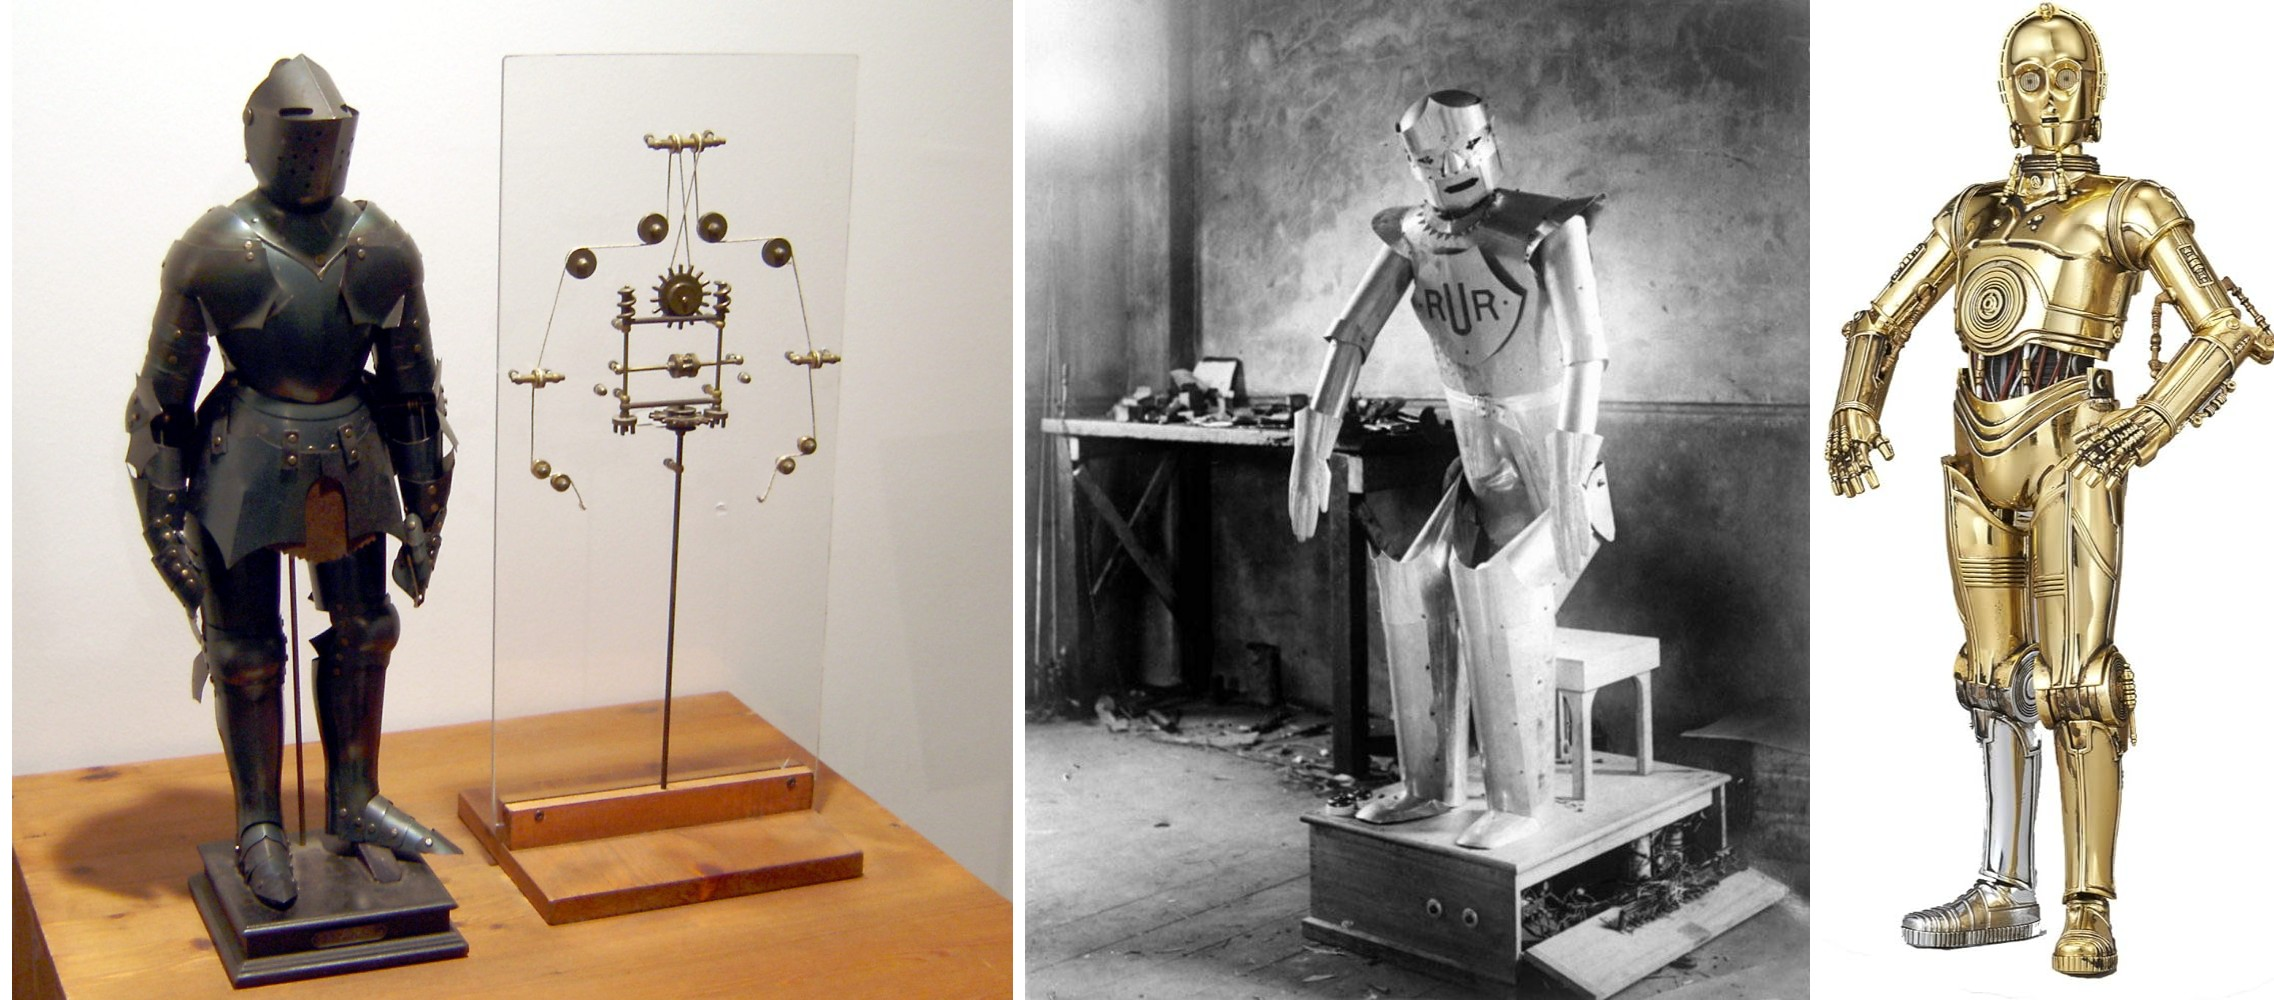
\includegraphics[width=\textwidth]{figures/01-introduction/robot-history.jpg}
    \caption{The Da Vinci robot \cite{Moran2006TheDaVinciRobot}.
        Rossum's Universal Robots \cite{Capek1920RUR}.
        C-3PO Star Wars \cite{StarWars1977}.
    }
    \label{fig:introduction:robots-in-history}
\end{figure}

\begin{figure}
    \centering
    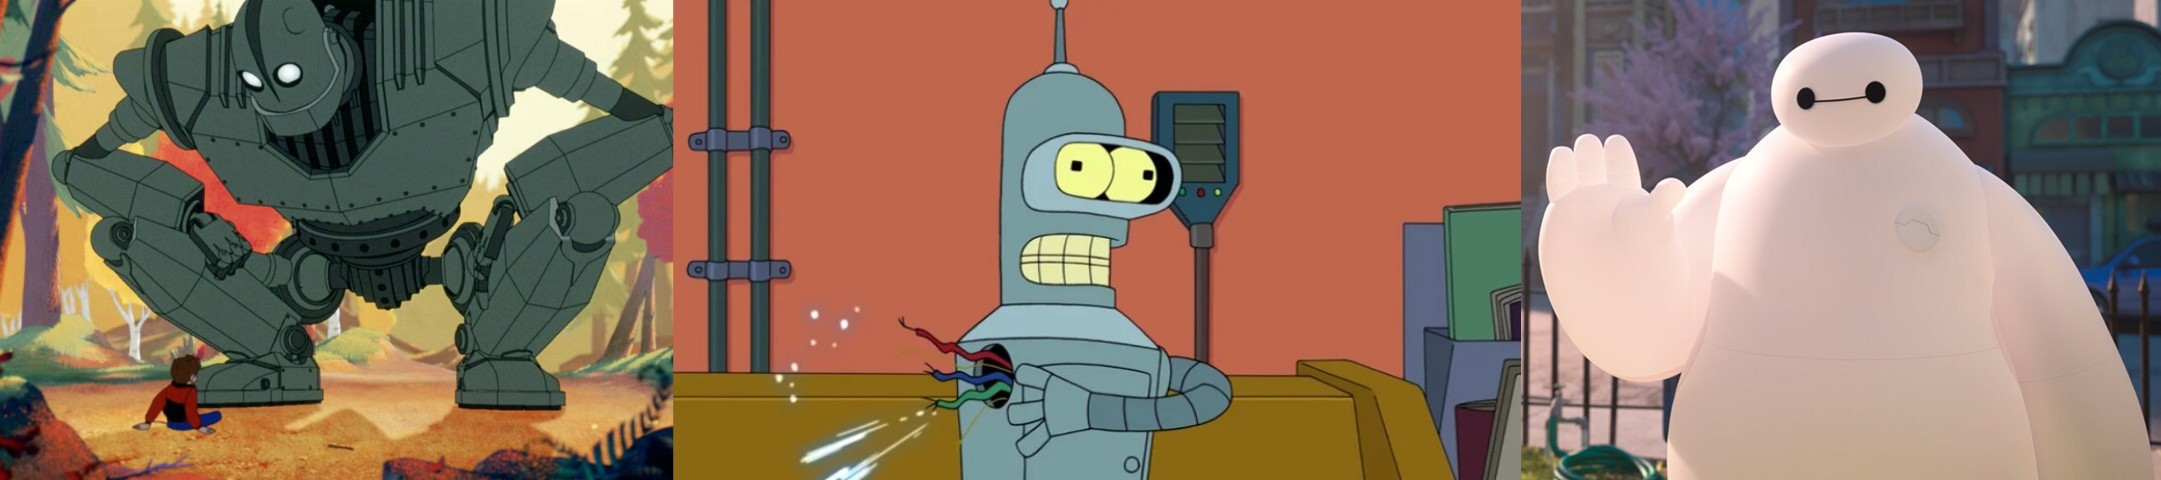
\includegraphics[width=\textwidth]{figures/01-introduction/robots-in-animation.jpg}
    \caption{The Iron Giant \cite{TheIronGiant1999}.
        Bender Futurama \cite{Futurama1999}.
        Baymax Big Hero 6 \cite{BigHero62014}.
    }
    \label{fig:introduction:robots-in-animation}
\end{figure}

\begin{figure}
    \centering
    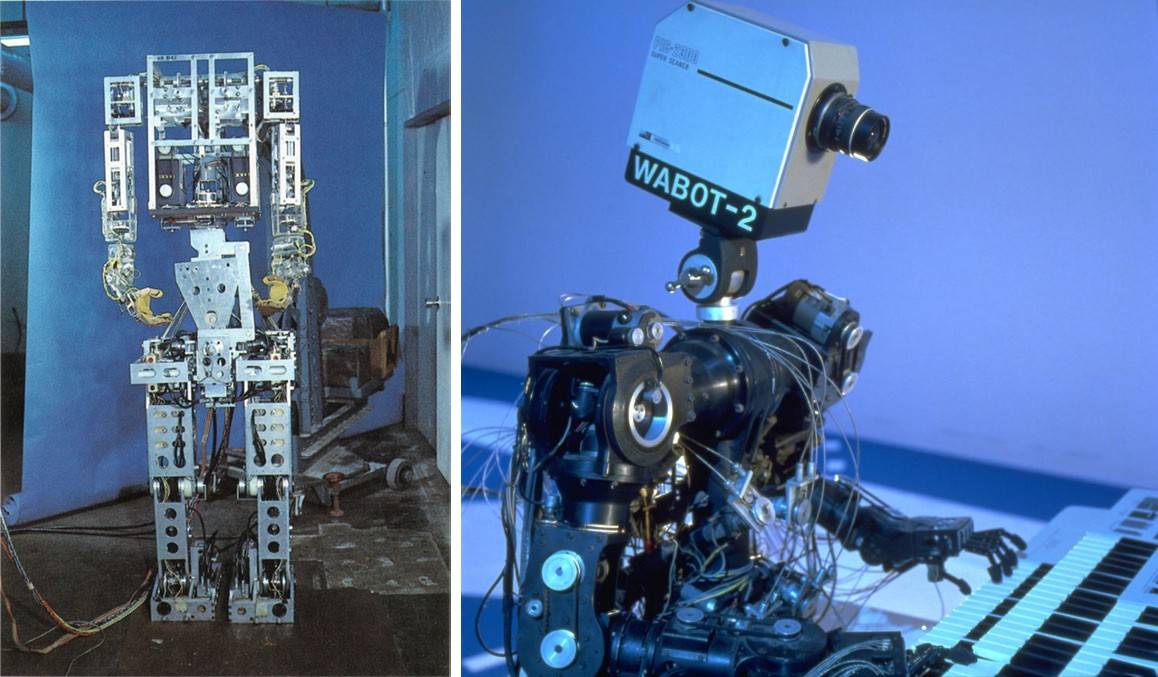
\includegraphics[width=0.7\textwidth]{figures/01-introduction/WABOTs.jpg}
    \caption{WABOT-1 \cite{Kato1973TheWABOT1}. WABOT-2 \cite{Kato1987WABOT2}.}
    \label{fig:introduction:WABOTs}
\end{figure}

\begin{figure}
    \centering
    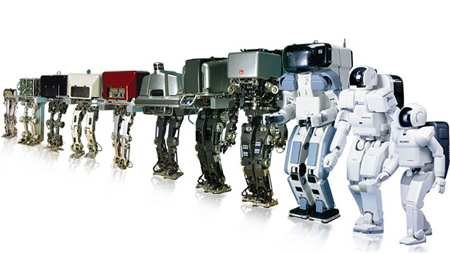
\includegraphics[width=0.7\textwidth]{figures/01-introduction/The-ASIMO-humanoid-robot-history.png}
    \caption{From Honda E0 to ASIMO \cite{Shigemi2019ASIMOandHumanoidRobotResearchatHonda}.}
    \label{fig:introduction:ASIMO-humanoid-history}
\end{figure}

\begin{figure}
    \centering
    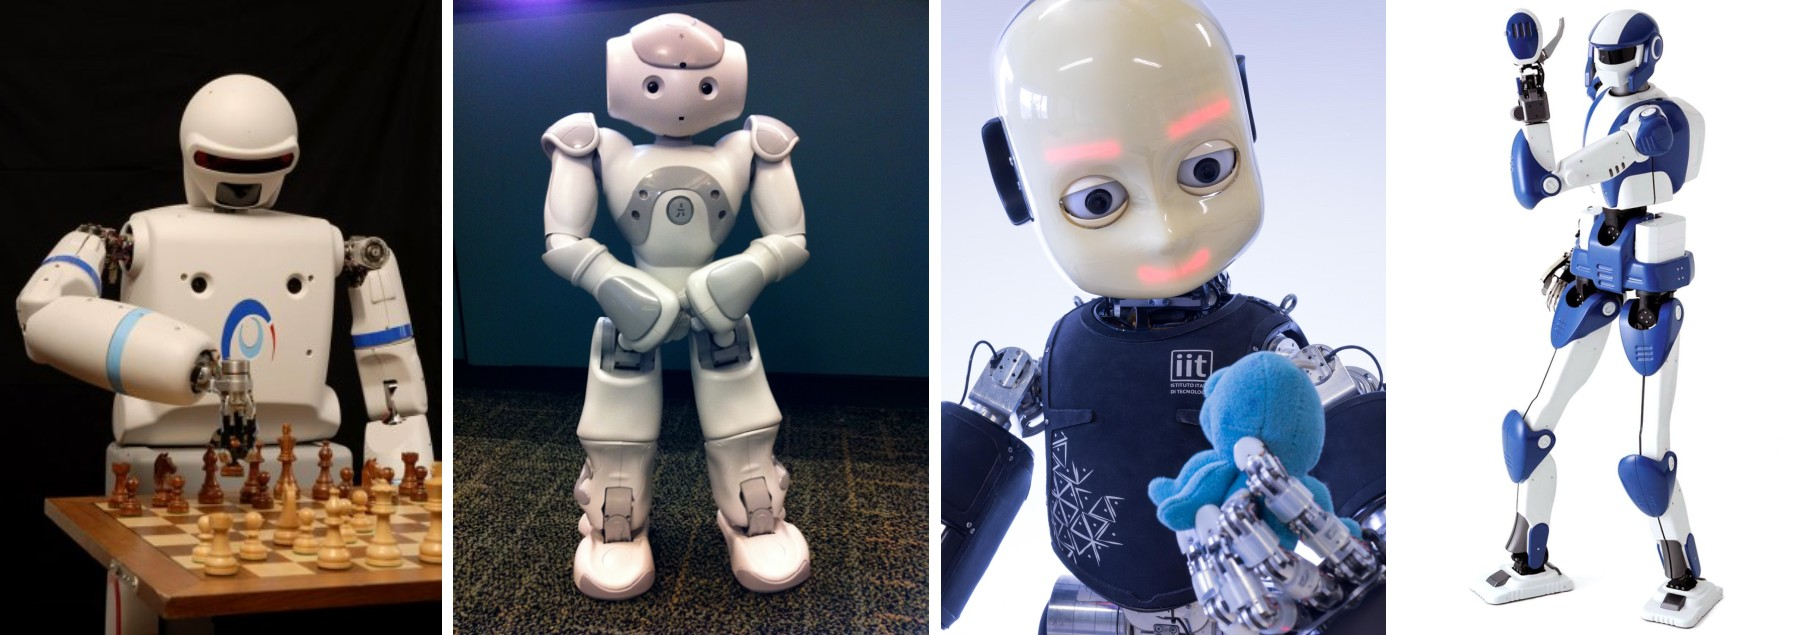
\includegraphics[width=\textwidth]{figures/01-introduction/robots-in-2000.jpg}
    \caption{Aldebaran NAO \cite{Gouaillier2008NAOHumanoid}.
        PAL Robotics REEM-B \cite{Tellez2008REEMB}.
        iCub \cite{Metta2010iCubHumanoid}.
        HRP-4 \cite{Kaneko2011HRP4}.
    }
    \label{fig:introduction:robots-in-2000}
\end{figure}

\begin{figure}
    \centering
    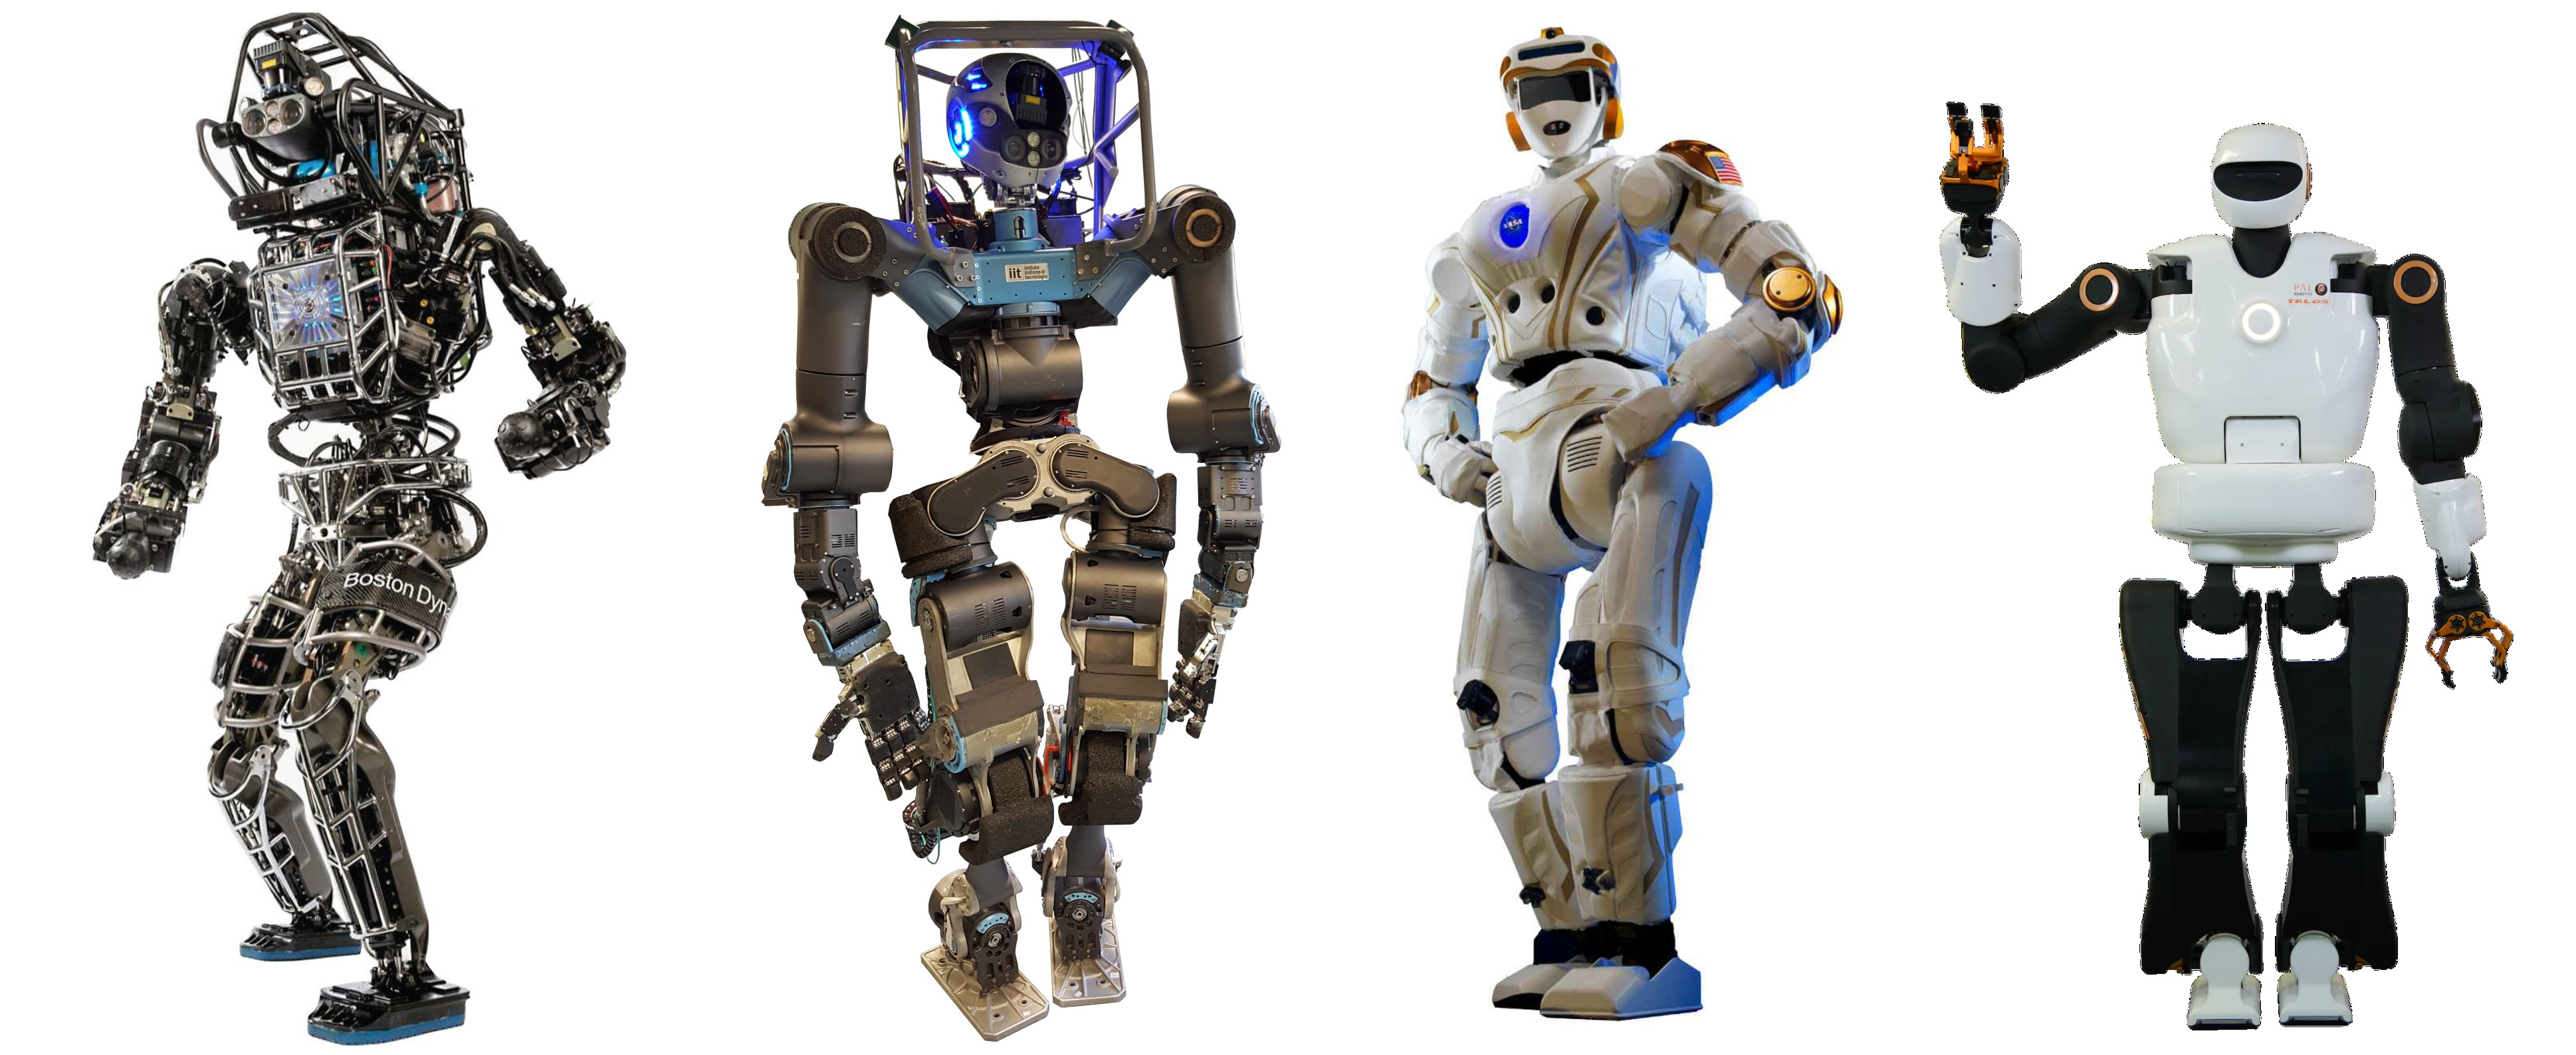
\includegraphics[width=\textwidth]{figures/01-introduction/robots-in-2010.jpg}
    \caption{Boston Dynamics ATLAS. WALK-MAN \cite{Tsagarakis2017WALKMAN}.
        NASA Valkyrie \cite{Radford2015Valkyrie}.
        PAL Robotics TALOS \cite{Stasse2017TALOS}.}
    \label{fig:introduction:robots-in-2010}
\end{figure}

\begin{figure}
    \centering
    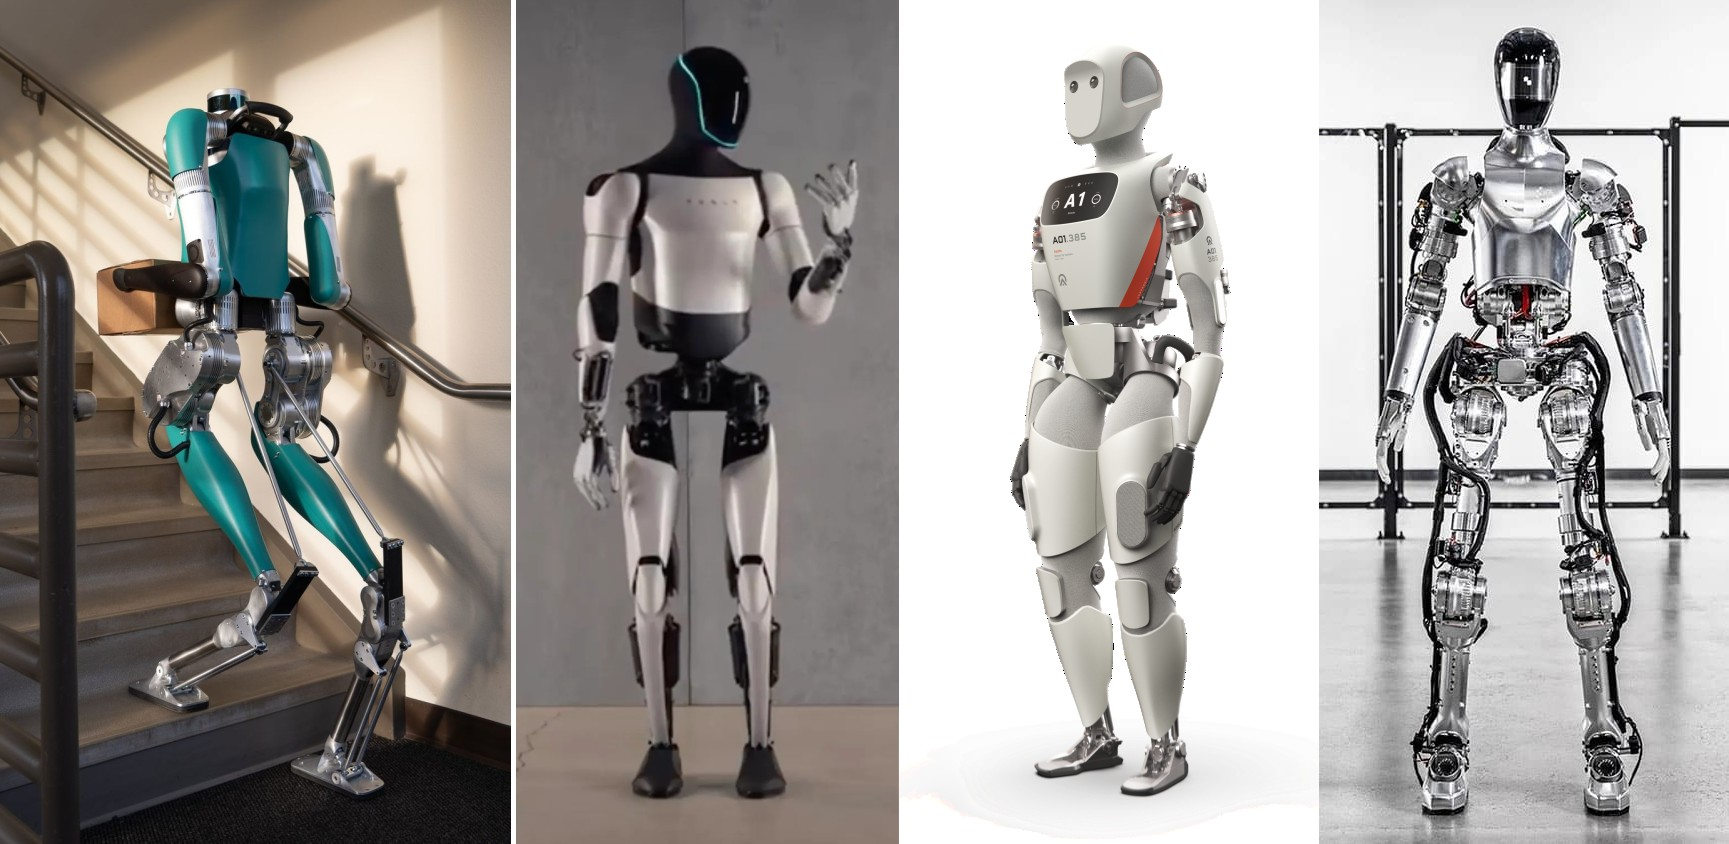
\includegraphics[width=\textwidth]{figures/01-introduction/robots-in-2020.jpg}
    \caption{Digit by Agility Robotics. Optimus by Tesla. Apollo by Apptronik.
        Figure 01 by Figure AI.
    }
    \label{fig:introduction:robots-in-2020}
\end{figure}

\begin{figure}
    \centering
    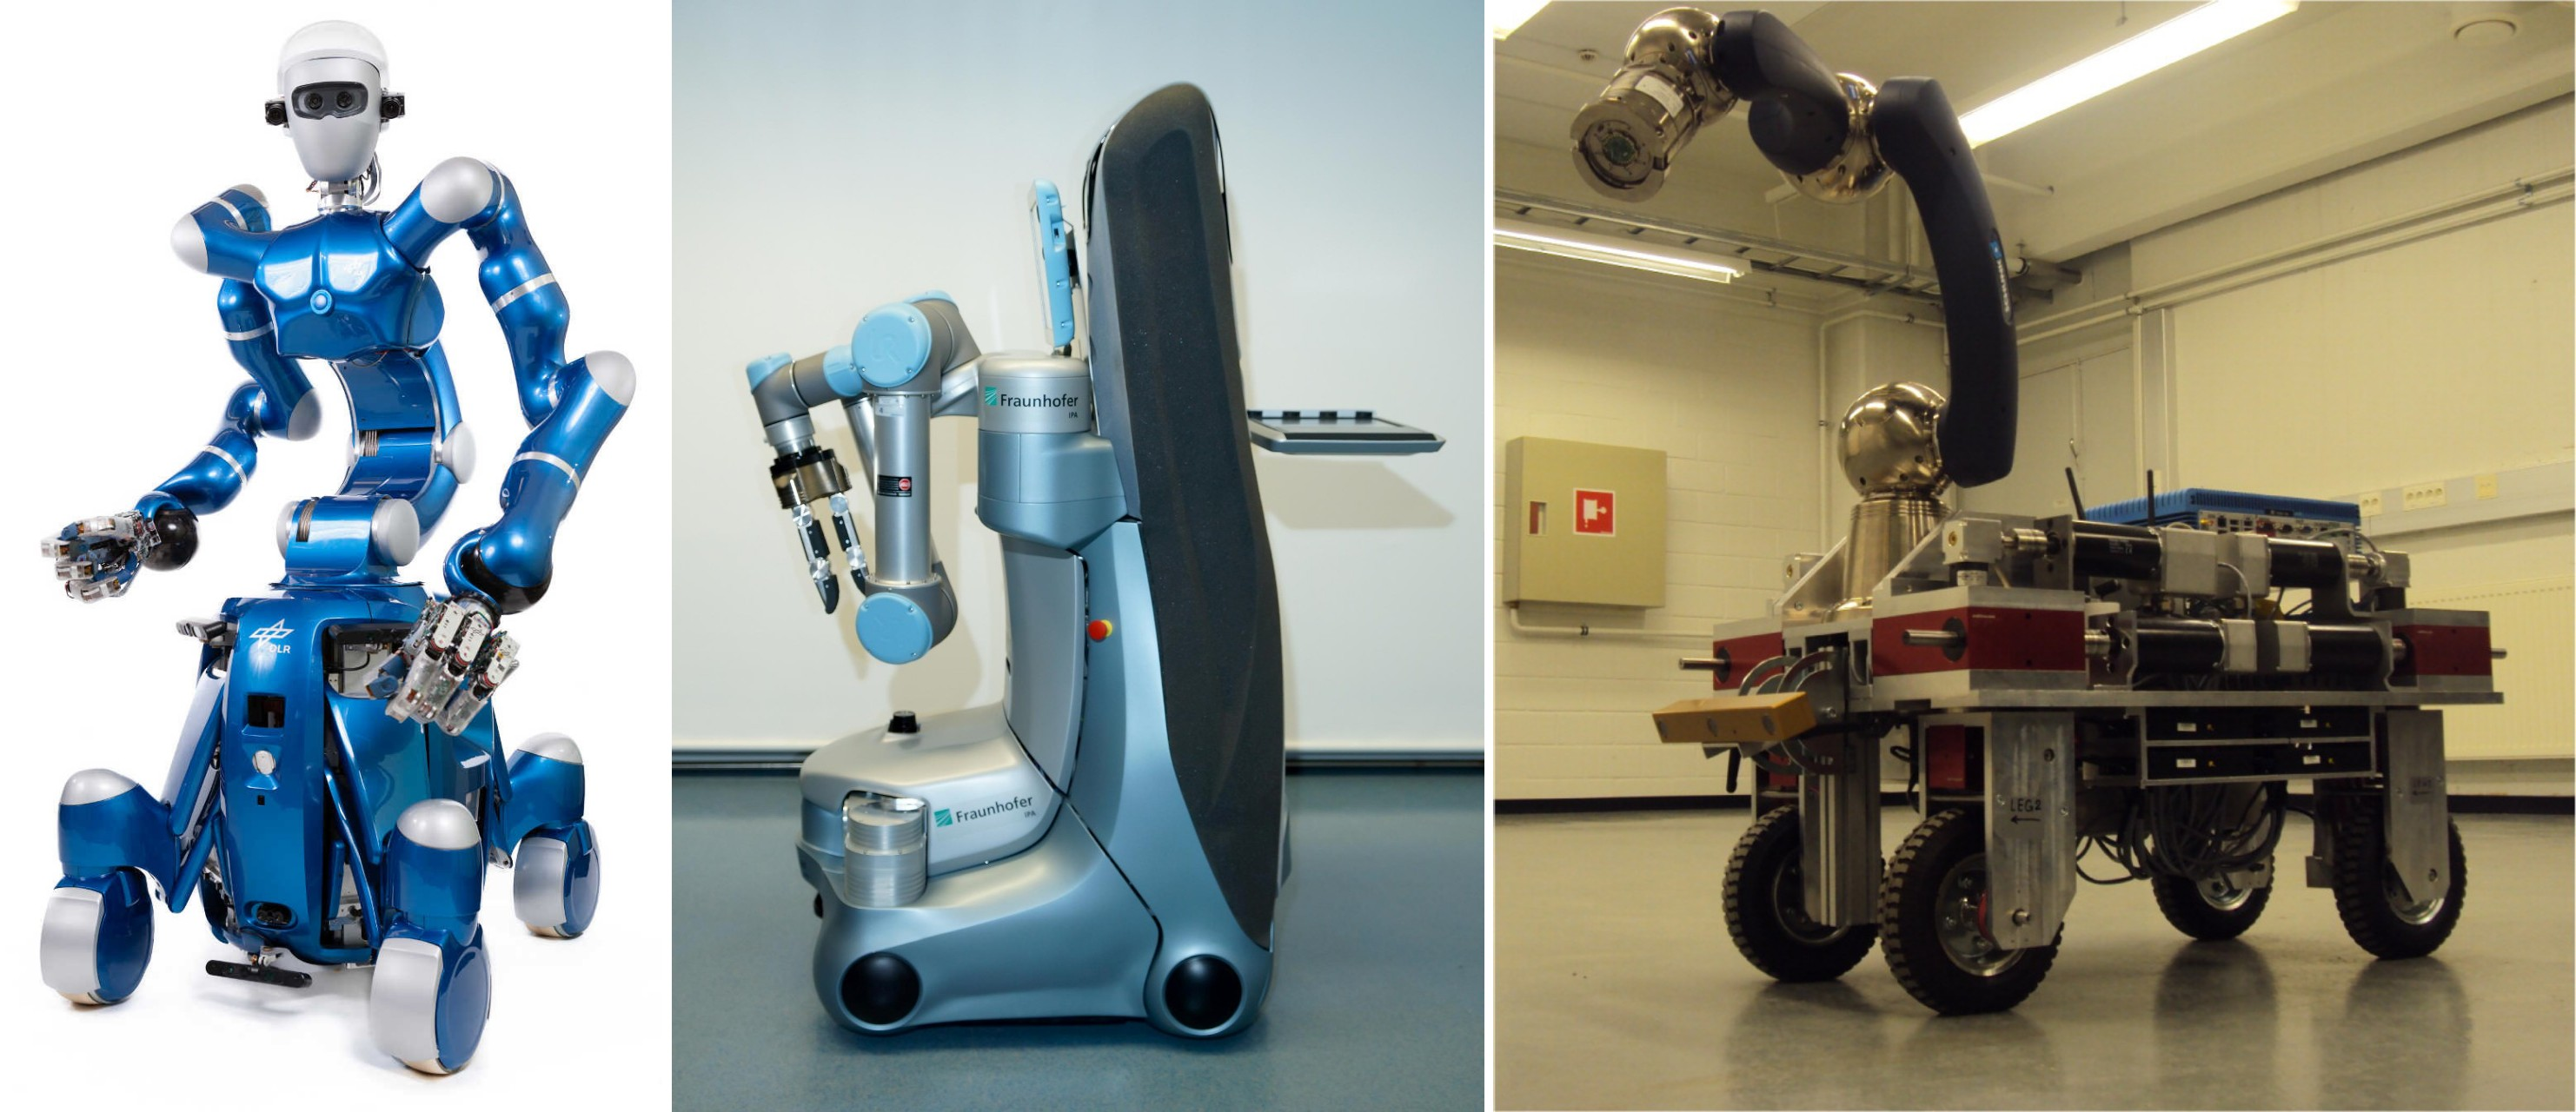
\includegraphics[width=\textwidth]{figures/01-introduction/SWMRs-1.jpg}
    \caption{Rollin' Justin \cite{Fuchs2009RollinJustin}.
        Care-O-bot 3 \cite{Graf2009Care-O-bot3}.
        iMoro \cite{Oftadeh2013iMoro}.}
    \label{fig:introduction:SWMRs-1}
\end{figure}

\begin{figure}
    \centering
    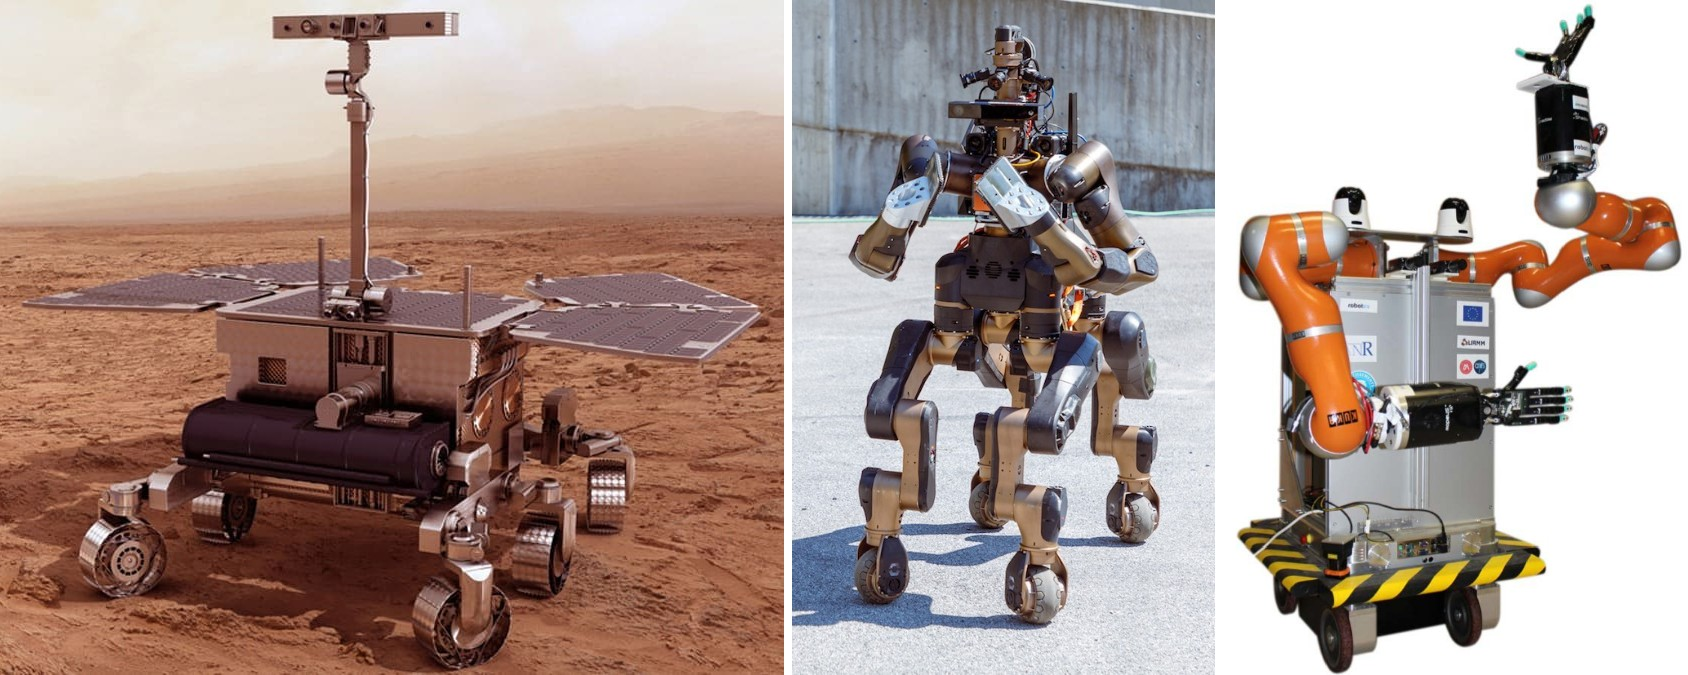
\includegraphics[width=\textwidth]{figures/01-introduction/SWMRs-2.jpg}
    \caption{ExoMars \cite{Poulakis2015ExoMarsMobilitySubsystem}.
        CENTAURO \cite{Kashiri2019Centauro}.
        BAZAR \cite{Cherubini2019ACR}.
    }
    \label{fig:introduction:SWMRs-2}
\end{figure}

\chapter{Literature review}
\label{ch:literature-review}
In this chapter, we give an overview on the literature of locomotion for
humanoid robots and motion control for
steerable wheeled mobile robots (SWMRs). In the first part of 
the chapter, we introduce the problems of 
gait generation, footstep planning, sensor-based locomotion, and footstep and 
timing adaptation for humanoids robots. In the second part of the chapter,
we study motion control algorithms for SWMRs.

\section{Humanoid robots}
\subsection{Gait generation}
In order for humanoid robots to successfully complete their tasks, they need to 
maintain balance at all times. The problem of gait generation consists in the
generation of trajectories that keep the robot balanced, and the realization of 
such trajectories on the humanoid itself. The most common type of gaits studied for 
humanoids are \textit{walking} and \textit{running}.
In this section, we briefly review the main 
scientific contributions to the problem of walking gait generation in 
planar and 3D environments.

Humanoid walking can be \textit{static} or \textit{dynamic}. In case of planar
contacts, in static walking, the 
projection of the \textit{Center of Mass} (CoM) lies within the
\textit{support polygon},
defined as the convex hull of the contact points. In dynamic walking, 
it is the \textit{Zero-tilting Moment Point} (ZMP) \cite{Vukobratovic1972ZMP},
defined as the point 
where the moment of the contact wrench aligns with the normal of the contact 
surface \cite{SardainBessonnet2004}, which lies within the support polygon.
In case of non-coplanar contacts,
an algorithm for testing static equilibrium has been developed by Bretl in
\cite{Bretl2008TestingStaticEquilibriumforLeggedRobots}, while for dynamic
walking, a more general
condition on the ZMP has been presented by Caron in
\cite{Caron2017TRO}.

Because of the complex nonlinear dynamics of the humanoid, the problem of gait 
generation is typically decomposed into two sub-problems: trajectory generation and 
whole-body trajectory tracking. The problem of trajectory generation is 
usually solved considering a simplified dynamics, such as the \textit{Centroidal
Dynamics} (the dynamics of the humanoid projected at its CoM)
\cite{Orin2013CentroidalDynamics} or the \textit{Linear Inverted Pendulum} (LIP)
\cite{Kajita1991LIP}. The problem of trajectory tracking is solved with a 
kinematic controller, typically implemented as a
stack-of-tasks \cite{Escande2014IJRR}, and solved through a hierarchy of 
Quadratic Programming (QP) problems.

The LIP relates the CoM to the ZMP through a linear dynamics, proving a 
theoretical tool that can be used for the generation of walking gait in 
real-time \cite{Sugihara2002ICRA}. More advanced techniques for the control 
of the ZMP can be found in \cite{Kajita2003BipedWalkingPatternGeneration}, which
presents a walking pattern generation scheme using preview control, or in
\cite{Wieber2006LMPCWalking}, which develops a Linear Model Predictive Control
scheme. In particular, the latter adopted a Cart Table model
\cite{Kajita2016IntroductiontoHumanoidRobotics}, minimizing the CoM jerk while enforcing the dynamic balance
condition (ZMP within the support polygon) as a constraint. This technique
was further developed taking into account automatic footstep placement
\cite{Herdt2010OnlineWalkingMotionGenerationWithAFSP}, stability \cite{Sherikov2014Humanoids}
and recursive feasibility \cite{Ciocca2017Humanoids} of the MPC.

More recently, Scianca introduced
\textit{Intrinsically-Stable MPC} (IS-MPC) \cite{Scianca2016ISMPC, Scianca2020TRO},
a gait generation scheme which 
uses the LIP as prediction model, enforcing dynamic balance
by constraining the ZMP within the support polygon,
and using a stability constraint to ensure that the CoM does not diverge 
with respect to the ZMP \cite{Lanari2015Inversionbasedgaitgeneration}. IS-MPC,
which will be used for gait generation throughout this manuscript,
has been extended to uneven ground in \cite{Zamparelli2018SYROCO} by
considering a dynamic balance condition in 3D
\cite{Caron2017DynamicWalkingOverRoughTerrains, Sugihara2021ICRA}. Because
IS-MPC is formulated as a QP problem, it can be efficiently solved by a 
QP solver and deployed on a real robot.

\subsection{Footstep planning}
Gait generation schemes such as IS-MPC rely on \textit{footstep plans}, which specify 
how the walking should be performed at high level (where to place each footstep,
the trajectory of the swing foot, and the duration of single and double support
phases). Footstep plans can either be manually defined, or computed by a 
footstep planner. In this section we review the literature on footstep planners,
diving them in two categories. The first one will cover footstep planners 
employing continuous techniques (optimization-based),
while the second one will cover footstep planners employing discrete techniques
(deterministic and randomized approaches).

Planners based on continuous techniques compute sequences of footsteps via
optimization, treating their poses as continuous decision variables. 
Several methods in this category (e.g., \cite{Ibanez2014IROS, Hong2011TSMC,
Kasadei2021SNAS}) rely on the implicit assumption that the ground is completely
flat and, therefore, are not tailored for motion generation in 3D environments.
Explicit account of 3D environment is instead made in
\cite{Deits2014FootstepPlanningMIQCQP}: the ground surface is decomposed as a
set of convex regions (with the aid of a manual initialization phase) and
footsteps are placed by solving a mixed-integer quadratic problem (MIQP). 
A more recent work \cite{Song2021RAL} casts the MIQP into a $l_1$-minimization
problem: to reduce the computational complexity, a suboptimal solution is
found by considering only those regions that intersect with the reachable
workspace of the feet along a pre-planned trajectory for the floating base
of the robot.

Planners based on discrete techniques find a solution by searching among
particular sequences of footsteps. These sequences are generated by
concatenation of \emph{primitives}. A primitive is a displacement between two
consecutive footsteps, selected among a finite number of possible displacements
from a catalogue.

To search among all possible sequences, one possibility is to use a
deterministic approach (search-based), which is typically represented by a variant of A* \cite{Hart1968Astar}.
Chestnutt implemented the A* footstep planner in \cite{Chestnutt2005FootstepPlanningASIMO}
for the ASIMO humanoid robot \cite{Sakagami2002ASIMO}. The work has been later 
extended to adaptively extend the catalogue of primitives
\cite{Chestnutt2007AdaptiveActionModel} depending on the terrain.
Hornung implemented Weighted A* \cite{Pearl1984Heuristics},
ARA* \cite{Likhachev2003ARAstar} and R* \cite{Likhachev2008Rstar}
footstep planners with anytime 
replanning strategies in \cite{Hornung2012AnytimeSearchbasedFootstepPlanning}.
Replanning strategies using D* Lite \cite{Koenig2002Dlite} and AD*
\cite{Likhachev2005ADstar} have been respectively implemented in
\cite{Gairmort2011HumanoidNavigationwithDynamicFootstepPlans} and 
\cite{Hornung2012AdaptiveLevelofDetailPlanning}.
Although search-based algorithms have been applied to 3D environments
\cite{Griffin2019ICRA}, this kind of approach suffers from two main issues: the
performance strongly depends on the chosen heuristic, which is often difficult
to design, and node expansion can be very expensive when using a large set of
primitives, because it requires the evaluation of all possible successors.

An alternative option is to use a randomized approach (sampling-based) such as
a variants of the Rapidly-exploring Random Tree (RRT) algorithm \cite{LaValle1998RRT}. 
This has been first developed in \cite{Zeyang2009RRTFootstepPlanning,
Zeyang2011RRTFootstepPlanning} in 2D environments, and later applied in simple
3D environments \cite{Perrin2012TRO, Liu2012IROS}, showing
good performance both in planning and replanning for dynamic environments.
Recently, Ferrari \cite{Ferrari2019ECC} presented a RRT footstep planner 
for humanoid navigation in uneven terrain, which is integrated with IS-MPC.
Clearly the disadvantage of RRT over a deterministic approach is that it does
not account, at least in its basic form, for the quality of the footstep plan.

\subsection{Sensor-based locomotion}
So far, it was assumed that a complete knowledge of the environment is available
from the start, or that, in case of dynamic environment, changes to the latter
are readily communicated to the planner. However, this is not often the case in
practical situations. In fact, the environment could be unknown, either
partially or completely, and it must be reconstructed online with the aid of
on-board sensors.

Many existing methods exploit information acquired through on-board sensors to
identify planar surfaces that define safe regions where the robot can step onto
\cite{Gutmann2008EnvironmentMapGeneration, Biswas2012PlanarPolygonExtraction,
Deits2015ComputingLargeConvexRegions, Bertrand2020DetectingUsablePlanarRegions,
Mishra2021GPUAcceleratedRapidPlanarRegionExtraction}.
Such environment representation was used in combination with different kinds of
footstep planners, for example, based on simple geometric criteria
\cite{Okada2005ICRA}, A* \cite{Chestnutt2009IROS, Calvert2022BipedalWalkingoverRapidRegions}
and MIQP \cite{Fallon2015Humanoids}.   
Other methods maintain a more complete representation of the environment by
employing an elevation map \cite{Burgard2016WorldModeling}.
Examples can be found in \cite{Maier2013IROS, Stumpf2014Humanoids},
where ARA*-based approaches are used to plan footsteps on uneven ground; the
use of on-line information is aimed at improving the plan during the execution,
and not for replanning/extension using newly acquired information.
To achieve more flexibility in the on-line capabilities,
\cite{Karkowski2016Humanoids} proposed to use adaptive sets of possible foot
displacements in an A*-based planner, which proved to be effective in relatively
simple scenarios. Alternatively, \cite{Yamamoto2021AdvancedRobotics} proposed a
two-stage method that first finds a collision-free path for a bounding occupancy
volume and then computes a compatible sequence of footsteps, which is a
suitable technique as long as it is not necessary to traverse narrow passages.

\subsection{Footstep and timing adaptation}
The techniques discussed so far assume that the robot is not subject to strong 
disturbances. Nevertheless, in order for the humanoids to be deployed in
real-world scenarios, the presence of possible external forces must be taken 
into account. In principle, when subject
to external perturbations, the humanoid should be able to adapt the footstep plan
by changing the position and the timing of the footsteps.

Model Predictive Control schemes, in their basic form, allow to
perform real-time footstep position adaptation \cite{Herdt2010IROS} and obtain
reactive stepping so to reject pushes and impacts. However, in order to be
able to formulate the optimization problem as a Quadratic Program (QP),
constraints should be kept linear. For this reason, most schemes only adapt
footstep positions, leaving out footstep orientation and step timing, and not
considering the possibility to place footsteps on a different contact surface,
which is crucial when walking on uneven terrains.

Several efforts to improve this basic paradigm have been made. To include
automatic step timing adaptation, one could make the MPC nonlinear
\cite{Maximo2020MIQPAutomaticWalking,Bohorquez2017AdaptiveStepDuration,
Caron2017Whentomakeastep,Aurelien2014IROS}, denying real-time implementation or
requiring significant compromise in the control rate. A linear formulation is
obtainable by considering only the duration of the first footstep
\cite{Smaldone2021FeasibilityDrivenSTA,Khadiv2020StepTimingAdaptation}.
As for footstep orientation, this is also often ignored or planned independently
of the dynamics \cite{Herdt2010IROS}. To couple rotation decision with the
dynamics, some schemes employ non-convex optimization through nonlinear
\cite{Naveau2017RAL,Bohorquez2018AdaptiveStepRotation} or Mixed-Integer
Programming (MIP) \cite{Maximo2020MIQPAutomaticWalking}.
MIP can also be used to alternatively select between multiple convex regions
in which to place the footsteps, which would otherwise constitute a
non-convex constraint \cite{Aceituno2018RAL,Deits2014FootstepPlanningMIQCQP}.

\section{Motion control for steerable WMRs}
As already discussed in the previous chapter, mobile robots equipped with
multiple steerable wheels
have greater maneuverability than other wheeled mobile robots, since they are
omnidirectional \cite{RobuffoGiordano2009ICRA}. Besides, they can transport
higher payloads than omnidirectional robots equipped with mecanum wheels
\cite{Dickerson1991ControlOminidirectionalRobotwithMecaumWheels} or
with omni wheels \cite{Blumrich1974OmnidirectionalWheel}.
Nevertheless, modeling and controlling these robots is not
trivial due to the presence of kinematic singularities \cite{Sorour2017RAL},
which need to be handled with particular care, in order to avoid negatively
affecting their functionalities.

While many different approaches for modeling and control of steerable wheeled
mobile robots (SWMRs) exist in literature, none of them fully exploits their
potentialities. The main property of this kind of robots, indeed, is that their
instanteneous center of rotation (ICR) can be located anywhere on the plane
\cite{Campion1996TR}. This naturally leads to a parametrization based on
two-dimensional cartesian \cite{Sorour2016ICRA} or polar coordinates
\cite{Connette2008CDC}, which, however, leads to singularities that can make
it difficult to develop a control scheme. Sorour et al. \cite{Sorour2017RAL}
developed an ICR-based controller which handles singularities of the steering
axes. The work is further improved in \cite{Sorour2019RAS}, where the
singularity of the ICR at infinity is taken into account through a
complementary route strategy. While these approaches consider all singularities
of their parametrization, the velocity and acceleration bounds are only
considered at the level of the ICR, often resulting in undesired motions with
high velocity and high acceleration of the steerable wheels.
A singularity-free representation is presented in \cite{Ferland2010IROS}
and \cite{Clavien2018EstimationoftheICR}, and used in
of~\cite{Clavien2018ICRMotionControl}, where a free-of-singularity motion
controller is developed. Here, time scaling is performed to satisfy velocity
and acceleration constraints on the wheels, resulting however in
non-optimal motion execution.

\part{Motion generation for humanoid robots}
\chapter{Dynamics of humanoid locomotion}
Humanoid locomotion is based on exchanging contact forces with the environment,
which, thanks to friction, allows the robot to move. In order for the humanoid to
successfully complete locomotion tasks, such as walking or running, the motion
of the robot must be dynamically balanced, i.e., the robot must not fall.

To formally define the condition for dynamic balance, it is important
to understand the dynamics of humanoid locomotion. The motion of humanoid robots
is characterized by a sequence of foot contact phases. For example, a walking
gait is composed by \textit{double support} and \textit{single support} phases. During
double support, both feet are in contact with the ground. During single support,
only one foot is in contact with the ground, while the other one (the \textit{swing foot})
moves towards the subsequent footstep location. Each single and double support
phase has a duration, which determines how quickly the robot walks. Moreover,
the swing foot motion is described by a swing foot trajectory, which must be
collision free. Single and double support durations are chosen accordingly to 
the desired behavior and the phyisical limitations of the robot.

The problem of generation of a walking gait therefore depends on the
computation of contact forces that keeps the robot balanced during its motion.
In particular, contact forces must be such that they lie within the friction cone
relative to their contact surface, in order for the rigid body in contact not to slip. 
In literature, this condition is often simplified by assuming sufficient (or
infinite) friction, and it allows to focus only on unilaterality of contact.
This makes it possible to define a condition on the zero-tilting moment point
(ZMP), which must lie within a \textit{support region} during locomotion. This
support region is called \textit{support polygon} when walking on flat ground,
and it is defined as the convex hull of all contact points.

In this chapter, we will define a condition of dynamic balance that can be
used for walking over terrains composed of stairs. To do so, we will first introduce the 
\textit{Lagrangian dynamics} of the humanoids, which fully describes the evolution
of the system through exchange of forces with the environment. We will then 
consider the \textit{centroidal dynamics} of the system, which is the 
dynamics of the humanoid project at the center of mass (CoM). The centroidal
dynamics allows us to introduce template models such as the Variable-Height
Inverted Pendulum (VH-IP) and Linear Inverted Pendulum (LIP), which can be used to generate
a walking gait in real-time. In particular, in this manuscript the LIP model
will play a fundamental role, as it will be used to design a control framework
for humanoid walking on stairs.

\section{Lagrangian dynamics}
\label{sec:lagrangian-dynamics}
Consider a humanoid robot as an open kinematic chain composed of $n+1$ rigid bodies
(\textit{links}), connected by $n$ \textit{joints}. We define the \textit{joint
configuration} of the robot\footnote{Note that, while this definition of
joint configuration considers
humanoids composed only by revolute joints, the presented analysis is valid also for
robots composed by prismatic joints, or a combination of both.} as $\bm{q}_j \in \left(\mathrm{SO}(2)\right)^n$, and assume they
are actuated by a torque $\bm{\tau} \in \mathbb{R}^n$. The root of the tree defining the
kinematic chain represents the \textit{floating base} link, as it is not fixed to the
world frame. The \textit{floating base configuration} is parametrized by
$\bm{q}_b \in \mathrm{SE}(3)$, and it is composed by the position
$\bm{p}_b \in \mathbb{R}^3$ and the orientation $\bm{\theta}_b \in \mathrm{SO}(3)$
of the floating base itself. We define the configuration of the robot as
\begin{equation*}
    \bm{q} =
    \begin{bmatrix}
        \bm{q}_b \\ \bm{q}_j
    \end{bmatrix} \in \mathrm{SE}(3) \times \left(\mathrm{SO}(2)\right)^{n}.
\end{equation*}
As already mentioned before, humanoid robots move by interacting with the 
environment through the exchange of contact forces. Let $\bm{f}_k \in \mathbb{R}^3$
be the unilateral contact force exchanged with a contact surface
with normal $\bm{n}_k$ at the $k$-th 
contact point $\bm{p}_k\in\mathbb{R}^3$. Unilaterality of $k$-th contact is formally
defined by
\begin{equation*}
    \bm{n}_k^T \bm{f}_k > 0,
\end{equation*}
and it describes the impossibility of pulling on the ground. Moreover, we
assume constant contact phase, hence not considering impact dynamics, which
would make the model hybrid.

The equation of motion of the humanoid \cite{Sugihara2020DynamicsofHumanoidRobots}
is characterized by the following Lagrangian dynamics:
\begin{equation}
    \begin{bmatrix}
        \bm{M}_u \\ \bm{M}_a
    \end{bmatrix} \ddot{\bm{q}} +
    \begin{bmatrix}
        \bm{c}_u(\bm{q}, \dot{\bm{q}}) \\
        \bm{c}_a(\bm{q}, \dot{\bm{q}}) \\
    \end{bmatrix} =
    \begin{bmatrix}
        \bm{0} \\ \bm{\tau}
    \end{bmatrix} +
    \sum_{k=1}^{K}
    \begin{bmatrix}
        \bm{J}_{k, u}^T \\ \bm{J}_{k, a}^T
    \end{bmatrix}
    \bm{f}_k,
    \label{eq:equation-of-motion-humanoids}
\end{equation}
where $\bm{M}$ is the inertia matrix, $\bm{b}$ encodes Coriolis, centrifugal
and gravitational terms, and $\bm{J}_k$ is the contact Jacobian relative to
the $k$-th contact point $\bm{p}_k$. Note that the structure of the
above dynamics highlights the \textit{underactuated} ($u$ subscript) and
the \textit{actuated} ($a$ subscript)
dynamics of the system, which respectively describe the evolution of the
floating base and the joints.

Note that, in order for the dynamics \eqref{eq:equation-of-motion-humanoids} to
be consistent, the contact mode must be fixed \cite{Balkcom2002Computingwrenchcones},
(which implies that bodies in contact must not roll or slide). A contact force $\bm{f}_k$ is
\textit{feasible} if it lies in the friction cone $\mathcal{C}_k$ directed by
the contact normal $\bm{n}_k$:
\begin{equation}
    \label{eq:feasible-contact-force}
    \| \bm{f}_k - (\bm{f}_k \cdot \bm{n}_k) \bm{n}_k \|_2 \le \mu_k (\bm{f}_k \cdot \bm{n}_k)
\end{equation}
with $\mu_k$ static friction coefficient.

In the following we will assume that there always exists joint torques
$\bm{\tau}$ that realize the actuated part of eq.
\eqref{eq:equation-of-motion-humanoids}.

\section{Centroidal dynamics}
The above hypothesis allows as to focus on the unactuated part of the equation
\eqref{eq:equation-of-motion-humanoids}, and define the
\textit{centroidal dynamics} \cite{Orin2013CentroidalDynamics} of the humanoid:
\begin{equation}
    \label{eq:centroidal-dynamics}
    \begin{bmatrix}
        m \ddot{\bm{p}}_C \\ \dot{\bm{L}}_C
    \end{bmatrix} =
    \begin{bmatrix}
        m \bm{g} \\ \bm{0}
    \end{bmatrix} +
    \sum_{k=1}^K
    \begin{bmatrix}
        \bm{f}_k \\ (\bm{p}_C - \bm{p}_k) \times \bm{f}_k
    \end{bmatrix},
\end{equation}
where $m$ is the total mass of the robot, $\bm{p}_C$ is the position of its
center of mass (CoM), defined as
\begin{equation*}
    \bm{p}_C =
    \frac{\sum_{i=1}^{n+1} m_i \bm{p}_{l_i}}{\sum_{i=1}^{n+1} m_i} =
    \frac{\sum_{i=1}^{n+1} m_i \bm{p}_{l_i}}{m},
\end{equation*}
with $\bm{p}_{l_i}$ and $m_i$ are respectively the position and the mass of the $i$-th link, 
$\bm{g} = (0 \; 0 \; {-g})^T$ is the gravity vector ($g=9.81$~[m/s$^2$]), $\bm{f}_k$ is the contact force
applied at a point with coordinates $\bm{p}_k$ over a contact surface with normal
$\bm{n}_k$, $K$ is the total number of contacts, and $\bm{L}_c$ is the angular
momentum of the robot taken at the CoM.

Let us define the \textit{gravito-inertial wrench} taken at point $O$ as
\begin{equation}
    \label{eq:gravito-intertial-wrench}
    \bm{w}_O^{\rm gi}
    =
    \begin{bmatrix}
        \bm{f}^{\rm gi}\\
        \bm{\tau}_O^{\rm gi}
    \end{bmatrix}
    =
    \begin{bmatrix}
        m \bm{g} - m \bm{\ddot{p}}_C \\
        (\bm{p}_C - \bm{p}_O) \times (m \bm{g} - m \bm{\ddot{p}}_C) - \bm{\dot{L}}_C
    \end{bmatrix}.
\end{equation}
Similarly, the \textit{contact wrench} $\bm{w}_O^{\rm c}$ can be defined as
\begin{equation}
    \label{eq:contact-wrench}
    \bm{w}_O^{\rm c}
    =
    \begin{bmatrix}
        \bm{f}^{\rm c} \\
        \bm{\tau}_O^{\rm c}
    \end{bmatrix}
    =
    \sum_{k=1}^K
    \begin{bmatrix}
        \bm{f}_k\\
        (\bm{p}_k - \bm{p}_O) \times \bm{f}_k
    \end{bmatrix}.
\end{equation}

Note that the centroidal dynamics \eqref{eq:centroidal-dynamics} can be
rewritten as a sum of the two above wrenches
\begin{equation}
    \bm{w}_O^{\rm gi} + \bm{w}_O^c = 0.
\end{equation}

\section{Zero-tilting moment point}
\label{sec:zero-tilting-moment-point}
Consider the gravito-inertial wrench defined in \ref{eq:gravito-intertial-wrench}. Zero-tilting moment points (ZMPs) are points $Z$ where the moment of the contact wrench aligns with the normal $\bm{n}$ of the contact surface \cite{SardainBessonnet2004}, i.e.,
\begin{equation}
    \label{eq:zmp-non-tilting-condition}
    \bm{\tau}_Z^{\rm gi} \times \bm{n} = \bm{0},
\end{equation}
which, using Varignon formula\footnote{A screw $\bm{w}_O =
(\bm{f},\bm{\tau}_O)$ represents the generalized force acting on a rigid body
\cite{Featherstone2007RigidBodyDynamicsAlgorithms},
and it is composed by a linear force $\bm{f}$ passing through $O$, together with the
total moment $\bm{\tau}_O$ about $O$. That total moment around any other point
$A$ can be computed using Varignon formula as $\bm{\tau}_A=\bm{\tau}_O+\bm{f}\times(\bm{p}_A-\bm{p}_O)$.}, can be rewritten as
\begin{equation*}
    \left(\bm{\tau}_O^{\rm gi} + (\bm{p}_O - \bm{p}_Z) \times \bm{f}^{\rm gi}\right) \times \bm{n} = \bm{0},
\end{equation*}
which, developing the triple cross product\footnote{The triple cross product
between three vectors $\bm{a}, \bm{b}, \bm{c} \in \mathrm{R}^n$ is defined as
the cross product of the vector $\bm{a}$ with the cross product of the other
two: $\bm{a}\times(\bm{b}\times\bm{c})=(\bm{a}\cdot\bm{c})\bm{b}-
(\bm{a}\cdot\bm{b})\bm{c}$. Note that, since the cross product is anticommutative,
the following holds:
($\bm{a}\times\bm{b})\times\bm{c}=-(\bm{c}\cdot\bm{b})\bm{a}+
(\bm{c}\cdot\bm{a})\bm{b}$.}, the above equation becomes
\begin{equation}
    \bm{\tau}_O^{\rm gi} \times \bm{n} - (\bm{n} \cdot \bm{f}^{\rm gi}) (\bm{p}_O - \bm{p}_Z) - \left(\bm{n} \cdot (\bm{p}_O - \bm{p}_Z)\right) \bm{f}^{\rm gi} = \bm{0}.
\end{equation}

Assuming that a point $Z$ lies on a plane with normal $\bm{n}$ intersecting the point $O$, i.e. $Z \in \Pi(O, n)$, the term $\bm{n} \cdot (\bm{p}_O - \bm{p}_Z) = 0$, and the above equation can be easily rewritten as
\begin{equation}
    \bm{p}_Z = \bm{p}_O + \frac{\bm{n} \times \bm{\tau}_O^{\rm gi}}{\bm{n} \cdot \bm{f}^{\rm gi}},
\end{equation}
finally defining the ZMP $Z$. Note that, more in general, there exists an infinity of ZMPs which lie on the non-central axis defined by \eqref{eq:zmp-non-tilting-condition}. For more details, please refer to \cite{SardainBessonnet2004}.

\subsection{Relationship between CoM, ZMP and angular momentum}
Consider the non-tilting condition of Eq. \eqref{eq:zmp-non-tilting-condition}. Using Varignon formula $\bm{\tau}_Z^{\rm gi} = \bm{\tau}_C^{\rm gi} + \bm{f}^{\rm gi} \times (\bm{p}_Z - \bm{p}_C)$, we have that
\begin{equation}
    \left(\bm{\tau}_C^{\rm gi} + \bm{f}^{\rm gi} \times (\bm{p}_Z - \bm{p}_C)\right) \times \bm{n} = \bm{0},
\end{equation}
which, computing the triple product, becomes
\begin{equation}
    \bm{\tau}_C^{\rm gi} \times \bm{n} - \left(\bm{n} \cdot (\bm{p}_Z - \bm{p}_C)\right) \bm{g}^{\rm gi} + (\bm{n} \cdot \bm{f}^{\rm gi}) (\bm{p}_Z - \bm{p}_C) = \bm{0}.
\end{equation}

Applying the definition of \textit{gravito-inertial wrench} of eq. \eqref{eq:gravito-intertial-wrench} and rearranging the terms, it is simple to prove \cite{Caron2017TRO} the following relationship between the CoM acceleration, the ZMP position and the angular momentum:
\begin{equation}
    \label{eq:relationship-com-zmp-angular-momentum}
    \ddot{\bm{p}}_C = \bm{g} + \frac{\bm{n} \cdot (\bm{\ddot{p}}_C - \bm{g})}{\bm{n} \cdot (\bm{p}_C - \bm{p}_Z)} (\bm{p}_C - \bm{p}_Z) + \frac{\bm{n} \times \bm{\dot{L}}_C}{m \left(\bm{n} \cdot (\bm{p}_C - \bm{p}_Z)\right)}.
\end{equation}
\section{Inverted pendulum models}
\subsection{Variable-Height Inverted Pendulum}
Consider again the centroidal dynamics of eq. \eqref{eq:centroidal-dynamics}
and assume that the rate of change of angular momentum is negligible (i.e.,
$\dot{\bm{L}}_C=\bm{0}$). We define the dynamics of the \textit{Variable-Height
Inverted Pendulum} (VH-IP) \cite{Koolen2016VHIP} as
\begin{equation}
    \label{eq:VH-IP}
    m \ddot{\bm{p}}_C = m \bm{g} + \bm{f}^{\mathrm{c}}.
\end{equation}

Note that, because $\dot{\bm{L}}_C=\bm{0}$, the contact force
$\bm{f}^{\mathrm{c}}$ can be parametrized \cite{Caron2020ICRA} as
\begin{equation}
    \label{eq:contact-force-with-LG-0}
    \bm{f}^{\mathrm{c}} = m \lambda(t) (\bm{p}_C - \bm{p}_Z),
\end{equation}
with $\lambda(t)$ natural frequency of the VH-IP (where we explicitely
denote the time dependency of lambda to highlight the nonlinearity in the
dynamics). Note that $\lambda(t) > 0$ because
of unilaterality of contact.
The dynamics of the VH-IP can be rewritten as
\begin{equation}
    \label{eq:VH-IP-LG-0}
    \ddot{\bm{p}}_C = \lambda(t) (\bm{p}_C - \bm{p}_Z) + \bm{g}
\end{equation}
by plugging the contact force \eqref{eq:contact-force-with-LG-0} into
eq. \eqref{eq:VH-IP}.

%During locomotion, since the the $\bm{f}^{\mathrm{c}}$ are such that its
%component along the $z$ axis is positive (i.e., $f_z^{\mathrm{c}}=
%\bm{e}_z^T \bm{f}^{\mathrm{c}} > 0$ with $\bm{e}_z = (0 \; 0 \; 1)^T$), from eq.
%\eqref{eq:contact-force-with-LG-0}, we have that
%\begin{equation*}
%    f_z^{\mathrm{c}} = m \lambda(t) (z_C - z_Z) > 0,
%\end{equation*}
%which implies that $z_C > z_Z$.

\subsection{Linear Inverted Pendulum}
\label{sec:DynamicsHumanoidLocomotion:LinearInvertedPendulum}
The dynamics of the VH-IP, as already mentioned, is nonlinear due to the
variable frequency $\lambda(t)$. In this
section, we derive the dynamics of the \textit{Linear Inverted Pendulum} (LIP)
\cite{Kajita2016IntroductiontoHumanoidRobotics}. To do so,
we constrain the vertical motion of the CoM \cite{Zamparelli2018SYROCO} so that
\begin{equation}
    \lambda(t) = \frac{\ddot{z}_C + g}{z_C - z_Z} =
    \frac{\bm{n} \cdot (\ddot{\bm{p}}_C - \bm{g})}{\bm{n} \cdot (\bm{p}_C - \bm{p}_Z)} =
    \eta^2,
\end{equation}
with $\eta$ an arbitrary constant. In this way,
the dynamics \eqref{eq:VH-IP-LG-0} becomes the dynamics of the LIP:
\begin{equation}
    \label{eq:LIPM}
    \ddot{\bm{p}}_C = \eta^2 (\bm{p}_C - \bm{p}_Z) + \bm{g},
\end{equation}
which is in equilibrium when the CoM and the ZMP are displaced by
$\bm{g}/\eta^2$ \cite{Cipriano2023RAS}. Here, the gravity vector $\bm{g}$
acts as a constant drift. Figure \ref{fig:LIPM-robot} shows the humanoid walking
under the above dynamics.

\begin{figure}
    \centering
    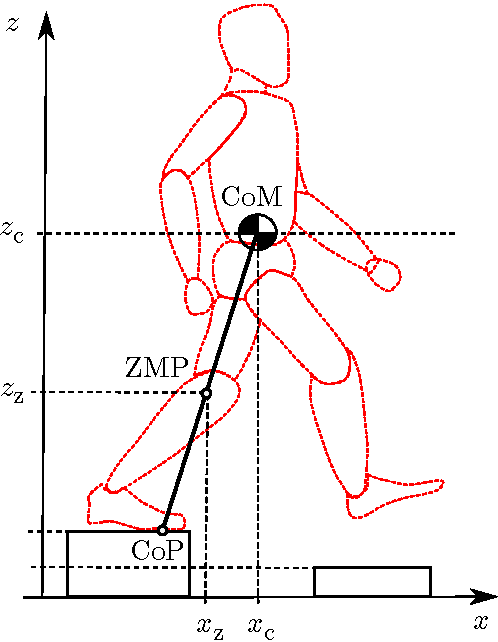
\includegraphics[width=0.45\textwidth]{figures/LIPM_robot.pdf}
    \caption{A humanoid walking under LIP dynamics. Note the positions of the CoM, the ZMP and the CoP, which lie on the same axis because of the assumption of conservation of angular momentum.}
    \label{fig:LIPM-robot}
\end{figure}

When walking on flat floor (a single contact surface with normal
$\bm{e}_z=(0 \; 0\; 1)^T$),
a common choice is to constrain the ZMP to lie on
a plane which coincides with the ground (i.e., without loss of generality
$z_Z=0$). As a consequence, the CoM is constrained to lie on a parallel plane
displaced by $h$ from the ZMP plane (i.e., $z_C=h$), and
the LIP dynamics further simplifies to the following dynamics:
\begin{align}
    \label{eq:LIPM-xy}
    \begin{split}
        \ddot{x}_C &= \eta^2 (x_C - x_Z) \\
        \ddot{y}_C &= \eta^2 (y_C - y_Z).
    \end{split}
\end{align}
Note that, in this particular case, the ZMP coincides with the center of
pressure (CoP), which is the point of application of the contact force
$\bm{f}^{\mathrm{c}}$ on the ground \cite{SardainBessonnet2004}.

The dynamics of eq. \eqref{eq:LIPM} is unstable \cite{Scianca2020TRO}. Indeed,
by rewriting it in state space form as
\begin{equation}
    \label{eq:LIPM-state-space}
    \begin{bmatrix}
        \dot{\bm{p}}_C \\ \ddot{\bm{p}}_C
    \end{bmatrix}
    =
    \begin{bmatrix}
        \bm{0}        & \bm{I} \\
        \eta^2 \bm{I} & \bm{0}
    \end{bmatrix}
    \begin{bmatrix}
        \bm{p}_C \\ \dot{\bm{p}}_C
    \end{bmatrix}
    +
    \begin{bmatrix}
        \bm{0} \\ -\eta^2 \bm{I}
    \end{bmatrix}
    \bm{p}_Z 
    +
    \begin{bmatrix}
        \bm{0} \\ \bm{g}
    \end{bmatrix},
\end{equation}
it is possible to see that the state matrix has eigenvalues in $\pm\eta$.
The instability of the system
can be further highlight by the following change of coordinates:
\begin{equation}
    \label{eq:LIP-change-of-coordinates}
    \begin{bmatrix}
        \bm{p}_u \\ \bm{p}_s
    \end{bmatrix}
    =
    \begin{bmatrix}
        \bm{I} &  \frac{1}{\eta} \bm{I} \\
        \bm{I} & -\frac{1}{\eta} \bm{I}
    \end{bmatrix}
    \begin{bmatrix}
        \bm{p}_C\\ \dot{\bm{p}}_C
    \end{bmatrix},
\end{equation}
which can be used to decouple the unstable and the stable subsystem. Indeed,
by taking the time derivative of eq. \eqref{eq:LIP-change-of-coordinates}, we
have
%\begin{align}
%    \dot{\bm{p}}_u &= \eta (\bm{p}_u - \bm{p}_Z) + \frac{\bm{g}}{\eta} \\
%    \dot{\bm{p}}_s &= \eta (\bm{p}_Z - \bm{p}_s) - \frac{\bm{g}}{\eta}
%\end{align}

\begin{equation*}
    \begin{bmatrix}
        \dot{\bm{p}}_u \\ \dot{\bm{p}}_s
    \end{bmatrix}
    =
    \begin{bmatrix}
        \eta\bm{I} &  \bm{0} \\
        \bm{0} & -\eta\bm{I}
    \end{bmatrix}
    \begin{bmatrix}
        \bm{p}_u \\ \bm{p}_s
    \end{bmatrix}
    +
    \begin{bmatrix}
        -\eta \bm{I} \\ \eta \bm{I}
    \end{bmatrix}
    \bm{p}_Z 
    +
    \begin{bmatrix}
        \frac{\bm{g}}{\eta} \\ -\frac{\bm{g}}{\eta}
    \end{bmatrix}
\end{equation*}

The coordinate $\bm{p}_u$ highlights the unstable component of the system
\eqref{eq:LIPM}, and it is referred to as \textit{divergent component of motion}
\cite{Englsberger2015TRO} or \textit{capture point}
\cite{Pratt2006CapturePoint}.

\section{Contact equilibrium}
%We are interested in defining the condition of equilibrium of a humanoid robot.
%As already stated in eq. \eqref{eq:feasible-contact-force}, a contact force
%$\bm{f}_k$ is feasible if it lies in the friction cone $\mathcal{C}_k$.
%Friction cones can be linearized by friction pyramids \cite{Caron2015RSS},
%obtaining a linear constraint on the contact forces. This constraint can be
%described in halfspace representation as
%\begin{equation}
%    \label{eq:friction-pyramid-halfspace}
%    \bm{F}_k \bm{f}_k \le \bm{0}.
%\end{equation}
%
%As explained in \cite{Caron2015RSS}, friction pyramid constraints can be used
%to compute the \textit{Contact Wrench Cone} (CWC), which can be described in
%halfspace representation as:
%\begin{equation*}
%    \bm{A}_O \bm{w}_O \le \bm{0}.
%\end{equation*}
%
%The CWC provides a necessary and sufficient condition for contact equilibrium of
%motions of the humanoid. Indeed, $\bm{w}_O$ belongs to the CWC if and only if
%there exists a set of contact forces $\{ \bm{f}_k \}$ which satisfy the
%centroidal dynamics equation \eqref{eq:centroidal-dynamics},
%the \textit{contact wrench} \eqref{eq:contact-wrench} and the friction pyramid
%constraints \eqref{eq:friction-pyramid-halfspace}.

We are interested in defining the condition of equilibrium of a humanoid robot.
While there exists a general condition on contact
equilibrium based on contact wrench cone \cite{Caron2015RSS}, in this manuscript
we assume that the friction coefficient defined in
\eqref{eq:feasible-contact-force} is sufficiently large to avoid slipping at the
contact surfaces.

This hypothesis allows us to focus on a simplified contact equilibrium
condition, which is relatively easy to deal with when developing a locomotion
scheme. In particular, consider the case of LIP dynamics of eq. \eqref{eq:LIPM}
with all contact forces directed towards the CoM, as described in
\cite{Sugihara2002ICRA}.
In this case, the contact forces can be rewritten as
\begin{equation}
    \label{eq:contact-force-towards-com}
    \bm{f}_k = \frac{\bm{p}_C - \bm{p}_k}{\| \bm{p}_C - \bm{p}_k \|_2} f_k,
\end{equation}
with $f_k>0$ the norm of $\bm{f}_k$. By plugging eq.
\eqref{eq:contact-force-towards-com} into eq.
\eqref{eq:centroidal-dynamics}, we obtain
\begin{equation}
    m \ddot{\bm{p}}_C = m \bm{g} + \sum_{k=1}^K \frac{\bm{p}_C - \bm{p}_k}{\| \bm{p}_C - \bm{p}_k \|_2} f_k.
\end{equation}
Moreover, using the dynamics of eq. \eqref{eq:LIPM}, we can obtain
obtain (after rearranging the terms), the following:
\begin{equation*}
    \bm{p}_Z = \bm{p}_C - \sum_{k=1}^K \frac{\bm{p}_C - \bm{p}_k}{\| \bm{p}_C - \bm{p}_k \|_2} \frac{f_k}{m \eta^2}.
\end{equation*}

Because of the assumption of sufficient joint torque actuation made in Sec.
\ref{sec:lagrangian-dynamics}, in principle, we could modulate $f_k$ to position
the ZMP within the area defined by the following set:
\begin{equation}
    \mathcal{Z} = \left\{ \bm{p}_Z \,\middle\vert\, \bm{p}_Z = \bm{p}_C + \sum_{k=1}^K \gamma_k (\bm{p}_k - \bm{p}_C), \; \gamma_k > 0  \right\},
    \label{eq:ZMP-polyhedral-cone}
\end{equation}
which is a polyhedral cone with apex $\bm{p}_C$ (Fig. \ref{fig:balance3D}), and
is known in literature as \textit{support region} \cite{Sugihara2021ICRA},
as it contains all feasible positions of the ZMP. Note that under dynamics
\eqref{eq:LIPM-xy}, the support region becomes the \textit{support
polygon}, which is defined as the convex hull of all contact points
\cite{SardainBessonnet2004}.

\begin{figure}
    \centering
    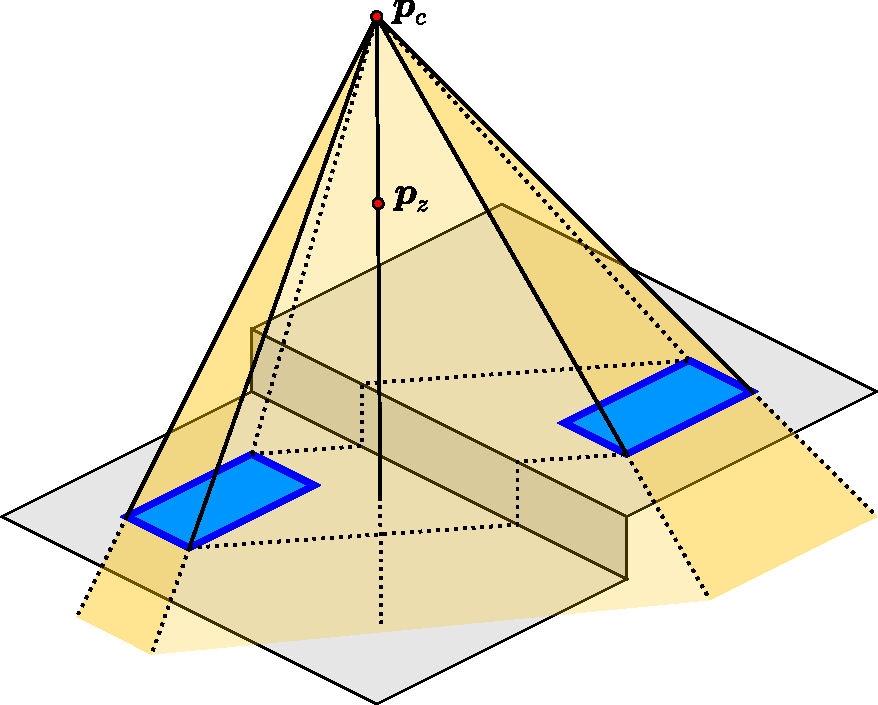
\includegraphics[width=0.6\textwidth]{figures/balance3d.pdf}
    \caption{3D balance: the ZMP $\bm{p}_Z$ must be inside the polyhedral cone $\mathcal{Z}$.}
    \label{fig:balance3D}
\end{figure}

Despite the above hypothesis on contact forces seems a strong assumption, it
has been used successfully for both walking and running tasks
\cite{Sugihara2002ICRA,Zamparelli2018SYROCO,Sugihara2021ICRA,Smaldone2022Running}. Moreover, when in
single support (or when all contacts are coplanar), the above condition is
always satisfied if $\dot{\bm{L}}_C=\bm{0}$
\cite{Caron2017DynamicWalkingOverRoughTerrains}.
\chapter{Gait generation via IS-MPC}
\label{sec:FAPA:GaitGeneration}
The gait generation module receives the planned footstep sequence ${\cal S}_f$ as input, and it is in charge of producing a CoM trajectory that the robot can safely track in order to step over said footstep sequence. Along the entire motion, dynamic balance must be maintained.

On flat ground, it is common to ensure dynamic balance as a geometric criterion, by requiring that the ZMP must always be inside the convex hull of contact surfaces, i.e., the \emph{support polygon}. Traditionally, the ZMP is assumed to be located on the ground plane, which is uniquely defined when the environment is flat.

In non-flat environments, there is no unique ground surface on which the ZMP can be assumed to be. However, the aforementioned criterion can be extended to these cases by allowing the ZMP to move in 3D \cite{SuImYaCa:2021}. The balance criterion is satisfied as long as the ZMP is inside a three-dimensional \emph{support region} $\mathcal{Z}$ that takes the shape of a pyramid (see Fig.~\ref{fig:FAPA:balance3d}). The vertex of this pyramid is the robot CoM, and the edges are the lines connecting the CoM to the vertexes of the convex hull of the contact surfaces.

In MPC, dynamic balance is enforced via constraints on the ZMP position. However, the 3D support region $\mathcal{Z}$ cannot be directly employed to enforce a ZMP constraint, because this would be nonlinear, meaning that the resulting optimization problem would not be in a standard linear-quadratic formulation. The cause of this nonlinearity is given by the fact that the vertex of the pyramid $\mathcal{Z}$ is the CoM. Since both the ZMP and the CoM depend on the decision variables of the QP, this would result in product between the decision variables themselves.

In order to avoid this, we will define a smaller region, independent of the CoM position, where the ZMP is allowed to be. Furthermore, we will prove that this region conservatively approximates the actual support region $\mathcal{Z}$, and thus that the balance condition is always satisfied under the imposed constraints.

In this section we will describe the MPC gait generation scheme that is used in the proposed formulation. In particular, we will derive the prediction model and define the constraints that ensure stability and dynamic balance. Finally, we will state the QP problem to be solved at each iteration, and give a sketch of the complete algorithm.

\section{Prediction model}

Control of the ZMP is achieved using a dynamic model relating the position of the latter to the position and acceleration of the CoM. This dynamic model can be derived by balancing moments on the humanoid as a whole, and assuming that the rate of change of angular momentum around the CoM can be neglected, leading to the situtation shown in Fig. \ref{fig:ISMPC:LIPM-robot}, where the Center of Pressure (CoP) is located on the corresponding patch, while the ZMP can be anywhere along the line joining the CoP and the CoM \cite{CaKh:17}.

With this in mind, denoting the CoM as $\bfp_c = (x_c \; y_c \; z_c)^T$ and the ZMP as $\bfp_z = (x_z \; y_z \; z_z)^T$, we get
\begin{equation}\begin{split}
(z_c - z_z)\ddot x_c &= (x_c - x_z)(\ddot z_c + g) \\
(z_c - z_z)\ddot y_c &= (y_c - y_z)(\ddot z_c + g) \\
\ddot{z}_c &= \frac{f_z}{m}-g,
\end{split}\end{equation}
where $g=-9.81$~[m/s$^2$] is the gravity acceleration, $f_z$ denotes the $z$-component of the ground reaction force, acting as an external input, and $m$ is the total mass of the robot.

This model exhibits a nonlinear coupling between the vertical and the horizontal components of $\bfp_c$ and $\ddot\bfp_c$. On flat ground, this nonlinearity is usually handled by assuming a constant CoM height, which leads to the well-known LIP model~\cite{KaKaKaFuHaYoHi:03}. In order to allow for vertical movement of the CoM, a different choice is made here, which is to constrain the motion of the CoM \cite{ZaScLaOr:18} to satisfy the relation
\begin{equation*}
    \frac{\ddot z_c + g}{z_c - z_z} = \eta^2,
\end{equation*}
where $\eta$ is a constant parameter.
The resulting dynamic model can be expressed in the form
\begin{equation}\label{eq:WoS:3dmodel}
\ddot \bfp_c = \eta^2(\bfp_c - \bfp_z) + \bfg,
\end{equation}
where $\bfg = (0 \; 0 \; {g})^T$ is the gravity acceleration vector. This model features a LIP-like dynamic behavior along all three axes. The only difference with respect to a standard LIP is given by the gravity vector $\bfg$ acting as a constant drift. This causes the system not to be in equilibrium when the CoM and ZMP coincide, but rather when they are displaced by $\bfg/\eta^2$.

\begin{figure}
    \centering
    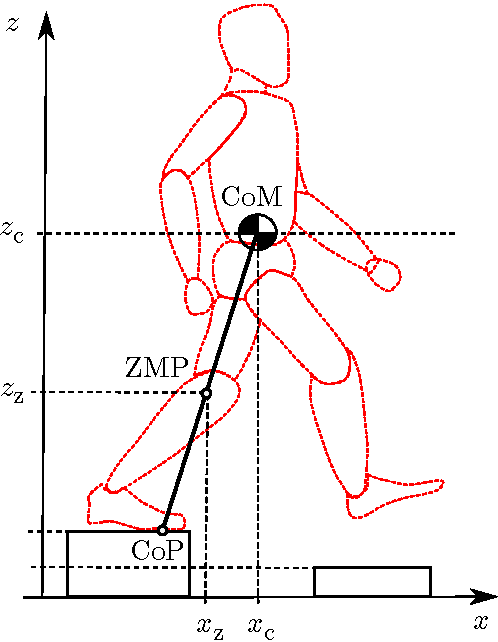
\includegraphics[width=0.4\textwidth]{figures/LIPM_robot.pdf}
    \caption{A humanoid walking on a world of stairs. Note the positions of the CoM, the ZMP and the CoP, which lie on the same axis because of the assumption of conservation of angular momentum.}
    \label{fig:ISMPC:LIPM-robot}
\end{figure}

The choice of restricting the available trajectories to those resulting in a constant $\eta$ allows to make the prediction model linear. If this restriction is removed, the model is referred to as Variable-Height Inverted Pendulum (VH-IP), which can be treated either as nonlinear or time-varying. This can allow for more general motions to be generated, e.g., running~\cite{Smaldone2022Running}, at the cost of a slightly more complex architecture. For the present case, where only walking is considered, the simpler model is preferred.

In order to obtain smoother trajectories, model (\ref{eq:WoS:3dmodel}) is dynamically extended to have the derivative of the ZMP $\dot \bfp_z$ as the input.
The gait generation scheme works over discrete time-steps of duration $\delta$, over which the input $\dot \bfp_z$ is assumed to be constant, i.e.,
\begin{equation*}
    \dot \bfp_z(t) = \dot \bfp_z^k,
\end{equation*}
for $t\in[t_k, t_{k+1})$. This prediction model is used to forecast the evolution of the system over a receding horizon window called the \emph{control horizon}, spanning a time $T_c=C\delta$. The number of steps that are contained, either fully or partially, within this control horizon is denoted as $F$.

\section{Stability constraint}
Model~(\ref{eq:WoS:3dmodel}) has a positive eigenvalue $\eta$, reflecting the intrinsic instability of the humanoid dynamics. Given this instability, it is not sufficient to generate a gait such that the ZMP is inside the support region, because the associated CoM trajectory might be divergent, making the motion unrealizable by the humanoid.
The role of the stability constraint is to enforce a condition on the unstable component of the dynamics in order to guarantee that the CoM trajectory does not diverge with respect to the ZMP.

The unstable component of system (\ref{eq:WoS:3dmodel}) is highlighted by the coordinate
\begin{equation*}
    \bfp_u = \bfp_c + \dot \bfp_c/\eta,
\end{equation*}
also referred to as \textit{divergent component of motion} \cite{EnOtAl:15} or \textit{capture point} \cite{PrCaDrGo:06}, that evolves according to the dynamics
\begin{equation}
\dot\bfp_u = \eta(\bfp_u - \bfp_z) + \frac{\bfg}{\eta}.
\end{equation}
Despite the instability, the evolution of the system is bounded if the following \emph{stability condition} is satisfied
\begin{equation}
\label{eq:WoS:stabilitycondition}
\bfp_u^k = \eta\int_{t_k}^{\infty}e^{-\eta(\tau - t_k)}\bfp_z(\tau) d\tau - \frac{\bfg}{\eta^2},
\end{equation}
where the superscript in ${\bfp}_u^k$ indicates that the variable is sampled at time $t_k$.

Condition~(\ref{eq:WoS:stabilitycondition}) is non-causal as it requires knowledge of the future ZMP trajectory $\bfp_z$ up to infinity. In order to derive a causal implementation, we split the integral at $t_{k+C}$. Of the two separate integrals that result, the first, over $[t_k, t_{k+C})$, can be expressed in terms of the MPC decision variables. A value for the second integral, over $[t_{k+C}, \infty)$, can be obtained by conjecturing a ZMP trajectory using information coming from the footstep plan.
This conjectured trajectory is called \emph{anticipative tail} and is denoted with $\tilde \bfx_z$. 
In \cite{ScDeLaOr:20}, the anticipative tail was used to prove recursive feasibility and stability of the MPC scheme.

The stability constraint is then written as
\begin{equation}\label{eq:WoS:stability_constraint}
\eta\int_{t_k}^{t_{k+C}}e^{-\eta(\tau - t_k)}\bfp_z d\tau = \bfp_u^k - \tilde \bfc^k + \frac{\bfg}{\eta^2}.
\end{equation}
where $\tilde \bfc^k$ is given by
\begin{equation}%\label{eq:WoS:stability_constraint}
\tilde\bfc^k = \eta\int_{t_{k+C}}^{\infty}e^{-\eta(\tau - t_k)}\tilde\bfp_z d\tau.
\end{equation}

Note that \cite{ScDeLaOr:20} considers the footstep plan to be available over a receding window called the \emph{preview horizon}. Here there is no need to make such an assumption, as the footstep plan is provided in its entirety, and once the goal is reached the robot comes to a complete stop.

Enforcing constraint (\ref{eq:WoS:stability_constraint}) allows to bound the displacement between CoM and ZMP. In fact, the value of the bound is almost identical in most practical situation, especially in view of the fact that the preview horizon is unlimited because the plan is completely known.

\textbf{From Humanoids 2023 stability constraint:}
[...] The second step is to make the decision variables appear explicitly, i.e., the ZMP velocities $\dot{\bm{X}}_z$ over the control horizon, by computing the integral over a piecewise linear ZMP trajectory. The final form of the constraint can be found in \cite{ScDeLaOr:20}. For the purpose of this analysis, we will use the compact expression
\begin{equation}\label{eq:FAPA:stability_constraint}
    \bfs^T \dot{\bm{X}}_z = b_x^k + x_u^k,
\end{equation}
where $\bfs\in\mathbb{R}^C$ and $b_x^k\in\mathbb{R}$ denote respectively a vector and a scalar whose explicit expressions can be recovered from the cited reference.


\section{ZMP constraint}
\subsection{Humanoids 2023}
\textbf{From Humanoids 2023 Stability constraint:} Relating the dynamics of the CoM to those of the ZMP is essential since the latter encodes information about the realizability of ground reaction forces, and thus provides a criterion for balance. 
% While on flat ground this criterion consists in keeping the ZMP within the support polygon of the robot, an extension for the 3D case is required. 
A common way to extend the basic 2D balance criterion consists in prescribing the 3D ZMP to be inside a 3D pyramid $\cal Z$ (see Fig.~\ref{fig:FAPA:balance3D}), having the base defined by the contact surfaces and the CoM vertex \cite{Sugihara2002ICRA, Cipriano2023RAS}.

\begin{figure}
    \centering
    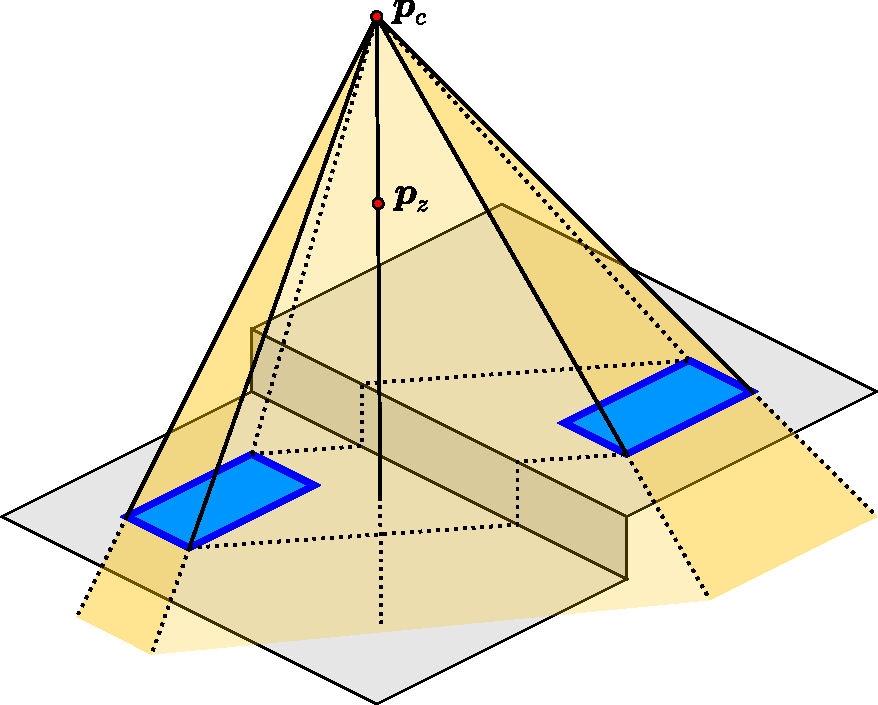
\includegraphics[width=0.55\textwidth]{figures/balance3d.pdf}
    \caption{3D balance: the ZMP $\bfp_z$ must be inside the polyhedral cone $\mathcal{Z}$.}
    \label{fig:FAPA:balance3D}
\end{figure}

The IS-MPC block receives the adapted subplan ${\cal P}^l$ and uses it to construct ZMP constraints. As described in the previous section, the criterion for balance is satisfied if the ZMP belongs to the pyramid $\cal Z$. However, enforcing this condition directly would lead to a nonlinear constraint in the MPC because the vertex of the pyramid is the CoM of the robot. Thus, we adopt a conservative approximation called the {\em moving constraint}.

The moving constraint requires for the ZMP to be at all times within a convex polyhedron of fixed shape, in our case a box of dimensions $d_x$, $d_y$ and $d_z$ centered in $\bfp_{\rm mc}=(x_{\rm mc}, y_{\rm mc}, z_{\rm mc})$, which we call the {\em moving box}. Along the prediction, the moving box can translate but not rotate, and its center moves in such a way that it is always fully contained within the 3D pyramid $\mathcal{Z}$ (see Fig. 5 in \cite{ZaScLaOr:18}). The vector $\bm{X}_{\rm mc}^{k+1} = (x_{\rm mc}^{k+1}, \dots, x_{\rm mc}^{k+C})^T$ collects the $x$ coordinate of the center of the moving box in the control horizon.

Because of its constant orientation in the prediction, at each time we can choose the orientation of the axes to align with the orientation of the moving box (taken as the orientation of the current support foot) and obtain a ZMP constraint that is decoupled along the 3 axes. Focusing on the component along $x$, we can write it as
\begin{equation}\label{eq:FAPA:ZMP_constraints}
    \bm{X}_z^{\rm m,k+1} \le \bm{X}_z^{k+1} \le \bm{X}_z^{M,k+1},
\end{equation}
where $\bm{X}_z^{k+1} = (x_z^{k+1}, \dots, x_z^{k+C})^T$ is a vector of predicted ZMP positions, and $\bm{X}_z^{\rm m,k+1}$ and $\bm{X}_z^{\rm M,k+1}$ are the ZMP bounds along the prediction.
By defining
\begin{equation*}
    \bm{Z} =
    \begin{pmatrix}
        \delta & 0 & \cdots & 0 \\
        \delta & \delta & \cdots & 0 \\
        \vdots & \vdots & \ddots & \vdots \\
        \delta & \delta & \cdots & \delta
    \end{pmatrix},
    \qquad
    \bm{z} =
    \begin{pmatrix}
        1 \\ 1 \\ \vdots \\ 1
    \end{pmatrix},
\end{equation*}
$\bm{X}_z^{k+1}$ can be expressed as
\begin{equation}
    \label{eq:FAPA:zmp-model-matrix-form}
    \bm{X}_z^{k+1} = \bm{Z} \dot{\bm{X}}_z^{k} + \bm{z} x_z^k,
\end{equation}
where $\dot{\bm{X}}_z^{k} = (\dot x_z^{k}, \dots, \dot x_z^{k+C-1})^T$ is the vector of ZMP velocities, i.e., the decision variables. The ZMP bounds along the prediction can be expressed as
\begin{equation}
    \bm{X}_z^{\rm m,k+1} = \bm{X}_{\rm mc}^{k+1} - \bfz \frac{d_x}{2}, \quad 
    \bm{X}_z^{\rm M,k+1} = \bm{X}_{\rm mc}^{k+1} + \bfz \frac{d_x}{2}.
\label{eq:FAPA:zmp_constraint_displacement}
\end{equation}
The center of the moving box $\bfp_{\rm mc}$ must be expressed in terms of the subplan $\mathcal{P}^l$. First we define the {\em piecewise-linear sigmoid} function 
\begin{equation*}
\sigma (t,t_i,t_f)=\frac{1}{t_f-t_i} \left(\rho(t-t_i)-\rho(t-t_f)\right),
%\label{eq:FAPA:sigma}
\end{equation*}
where $\rho(t)=t\delta_{-1}(t)$ is the unit ramp. $\sigma (t,t_i,t_f)$ is 0 before $t_i$,  1 after $t_f$, and it transitions linearly in the interval $[t_i,t_f]$. This function is useful to represent the transition between consecutive footsteps.

$\bm{X}_{\rm mc}^{k+1}$ can be written as
\begin{equation}
\label{eq:FAPA:mapping}
\bm{X}_{\rm mc}^{k+1} = \bm{M} \bm{X}_f^l + \bm{m}x_f^l,
\end{equation}
where $\bm{X}_{f}^{l} = (x_{f}^{l}, \dots, x_{f}^{l+F})^T$ collects the footstep positions. $\bm{M}\in\mathbb{R}^{C\times F}$ is a mapping matrix whose elements $M_{ij}$ are defined as
\begin{equation}\begin{split}
M_{ij} &= \sigma(t_{k+i}, t_s^{l+j},t_s^{l+j}+T_{\rm ds}^{l+j})\\ &- \sigma(t_{k+i}, t_s^{l+j-1},t_s^{l+j-1}+T_{\rm ds}^{l+j-1}),
\end{split}\end{equation}
and $\bfm\in\mathbb{R}^{C}$ is a vector whose elements $m_i$ are given by
\begin{equation*}
m_{i} = 1 - \sigma(t_{k+i}, t_s^{l},t_s^{l}+T_{\rm ds}^{1}),
\end{equation*}
where $t_s^l$ is the starting time of the $l$-th step and
\begin{equation*}
    t^j_s = t^l_s + \sum^{l+j-1}_{\lambda=l} \left(T_{\rm ds}^\lambda + T_{\rm ss}^\lambda\right).
\end{equation*}

\subsection{RAS 2023}
As already noted, the humanoid is balanced as long as the ZMP is inside the pyramid $\cal Z$, which is a nonlinear condition due to the vertex of the pyramid being at the CoM (Fig. \ref{fig:FAPA:balance3d}). To preserve linearity we consider a smaller allowed region for the ZMP, consisting in a box of fixed size with changing center and orientation. We refer to this as the {\em moving box}\footnote{Approximating the pyramidal region $\cal Z$ with a box might seem overly conservative. However, we argue that the neglected portion of the pyramid region is not crucial here, because large displacements of the ZMP in the $z$ direction would only be required to generate large vertical accelerations, which are not necessary in the considered setting (walking in a world of stairs). Clearly, less conservative approximations can still be envisaged and used for generating more dynamic motions.}, and we will prove that it conservatively approximates the support region, meaning that it is always contained inside the pyramid $\cal Z$.

The center $\bfp_{\rm mc}$ of the moving box is taken to be consistent with the pose of footstep $\bff^j$ during the $j$-th single support phase. At each time $t$, the center of the moving box $\bfp_{\rm mc}$ is expressed as
\begin{equation}\label{eq:WoS: moving constraint}
\bfp_{\rm mc}(t) = \Bigg\{
\begin{array}{ll}
\bfp^j & t\in [t_s^j, t_s^j + T_{\rm ss}^j) \\
(1-\alpha^j(t))\bfp^j + \alpha^j(t)\bfp^{j+1} & t\in [t_s^j + T_{\rm ss}^j, t_s^{k+1})
\end{array}
\end{equation}
where $j=0,\dots,F$ is a index over the footsteps within the control horizon, and $\alpha^j(t) = (t-t_s^j-T_{\rm ss}^j)/T_{\rm ds}^j$ denotes the time elapsed since the start of the double support phase, expressed as a fraction of the duration of the double support phase itself.

The ZMP position constraint is expressed as
\begin{equation}\label{eq:WoS:ZMP_constraint}
-\tilde\bfd /2 \le \bfp_z^{k+i} - \bfp_{\rm mc}^{k+i} \le \tilde\bfd /2
\end{equation}
where $\bfp_z^{k+i}$ and $\bfp_{\rm mc}^{k+i}$ respectively denote the ZMP and the center of the moving box sampled at time $t_{k+i}$, $\tilde \bfd = (\tilde d_x, \tilde d_y, d_z)^T$
is a vector collecting the dimensions of the moving box along all three axes.

The size of the moving box $\tilde \bfd = (\tilde d_x, \tilde d_y, d_z)^T$ is determined in such a way to always be contained inside the pyramid $\cal Z$. \textbf{TODO: either add Prop. 2 of RAS23 or eq. (12) of SYROCO18.}

\section{IS-MPC algorithm}
IS-MPC solves, at each time $t_k$, the following QP problem:
\begin{braced}
\begin{equation*}\begin{split}
\min_{\dot{\bm{X}}_\text{z}^k, \dot{\bm{Y}}_\text{z}^k, \dot{\bm{Z}}_\text{z}^k}
&\|\dot{\bm{X}}_z^k\|^2 + \|\dot{\bm{Y}}_z^k\|^2 + \|\dot{\bm{Z}}_z^k\|^2+\beta \|\bm{X}_z^{k+1} - \bfX_{\rm mc}^{k+1}\|^2 \\& + \beta \|\bm{Y}_z^{k+1} - \bfY_{\rm mc}^{k+1}\|^2 + \beta \|\bm{Z}_z^{k+1} - \bfZ_{\rm mc}^{k+1}\|^2 \\
\end{split}\end{equation*}
\hspace{0.25cm} subject to:
\begin{itemize}
\item ZMP constraints (\ref{eq:FAPA:ZMP_constraints})
\item stability constraints (\ref{eq:FAPA:stability_constraint})
\end{itemize}
\end{braced}

In the cost function, the first three terms act as regularization while the remaining attempt to bring the ZMP as close as possible to the center of the moving box, with a strength modulated by the weight $\beta$.

The first sample $\dot \bfp_z^k = (\dot x_z^k, \dot y_z^k, \dot z_z^k)$ of the optimal sequence is used to integrate the prediction model and the resulting CoM position $\bfp_c^{k+1}$ is sent to the kinematic controller together with a suitable swing foot trajectory that allows to reach the target footstep position at the proper time.

\section{Feasibility region}

The {\em feasibility region} is the region of the state space in which the IS-MPC optimization problem is feasible.

\begin{proposition}
\label{prop:feasibility}
IS-MPC is feasible at time $t_k$ if
\begin{align}
\label{eq:FAPA:mpc-feasibility-constraint}
\bm{s}^T \bm{Z}^{-1} (\bm{X}_z^{{\rm m}, k+1} \!-\! \bm{z} x_z^k)  \!&\le\! x_u^k \!+\! b_x^k \!\le\! \bm{s}^T \bm{Z}^{-1} (\bm{X}_z^{{\rm M}, k+1} \!-\! \bm{z} x_z^k),
\nonumber\\
\bm{s}^T \bm{Z}^{-1} (\bm{Y}_z^{{\rm m}, k+1} \!-\! \bm{z} y_z^k)  \!&\le\! y_u^k \!+\! b_y^k \!\le\! \bm{s}^T \bm{Z}^{-1} (\bm{Y}_z^{{\rm M}, k+1} \!-\! \bm{z} y_z^k),
\nonumber\\
\bm{s}^T \bm{Z}^{-1} (\bm{Z}_z^{{\rm m}, k+1} \!-\! \bm{z} z_z^k)  \!&\le\! z_u^k \!+\! b_z^k \!\le\! \bm{s}^T \bm{Z}^{-1} (\bm{Z}_z^{{\rm M}, k+1} \!-\! \bm{z} z_z^k).
\end{align}
\end{proposition}
{\em Proof}.
We focus the proof on the inequalities for the $x$ component, as the logic, for the other components is identical. The bounds of the feasibility region along $x$ are given by
\begin{align*}
x_u^{k,b1} &= \bm{s}^T \bm{Z}^{-1} (\bm{X}_z^{{\rm m}, k+1} - \bm{z} x_z^k) - b_x^k, \\
x_u^{k,b2} &= \bm{s}^T \bm{Z}^{-1} (\bm{X}_z^{{\rm M}, k+1} - \bm{z} x_z^k) - b_x^k.
\end{align*}
Then, if $x_u^k$ is inside the feasibility region, it is possible to express it as a convex combination of the two bounds, i.e.,
\begin{equation}\label{eq:FAPA:xu_convex}
x_u^k = \alpha x_u^{k,b1} + (1-\alpha)x_u^{k,b2}, \alpha \in [0, 1].
\end{equation}

Consider the following ZMP velocity trajectory:
\begin{equation}\label{eq:FAPA:candidate_trajectory}
\dot{\bm{X}}_z^k = \alpha \bm{Z}^{-1}(\bm{X}_z^{{\rm m}, k+1} - \bm{z} x_z^k) + (1-\alpha)\bm{Z}^{-1}(\bm{X}_z^{{\rm M}, k+1} - \bm{z} x_z^k).
\end{equation}
We will show that this particular trajectory satisfies both the stability constraint and the ZMP constraints. As for the stability constraint, multiply both sides of (\ref{eq:FAPA:candidate_trajectory}) by $\bm{s}^T$
% \begin{equation}
% \bm{s}^T\bm{\dot X}_z^k = \bm{s}^T(\alpha \bm{Z}^{-1}(\bm{X}_z^{{\rm m}, k+1} - \bm{z} x_z^k) + (1-\alpha)\bm{Z}^{-1}(\bm{X}_z^{{\rm M}, k+1} - \bm{z} x_z^k)),
% \end{equation}
and plug in the definitions of $x_u^{k,b1}$ and $x_u^{k,b2}$ to obtain
\begin{equation*}
\bm{s}^T\dot{\bm X}_z^k = (\alpha (x_u^{k,b1} + b^k_x)) + (1-\alpha)(x_u^{k,b2} + b^k_x)).
\end{equation*}
Using (\ref{eq:FAPA:xu_convex}), this is equivalent to the stability constraint (\ref{eq:FAPA:stability_constraint}).

To prove satisfaction of the ZMP constraint. Left-multiplying \eqref{eq:FAPA:zmp-model-matrix-form} by $\bm{Z}$, the chosen ZMP velocity trajectory can be rewritten as
\begin{equation*}
\bm{X}_z^k - \bm{z} x_z^k = \alpha (\bm{X}_z^{{\rm m}, k+1} - \bm{z} x_z^k) + (1-\alpha)(\bm{X}_z^{{\rm M}, k+1} - \bm{z} x_z^k),
\end{equation*}
which simplifies to
$\bm{X}_z^k = \alpha \bm{X}_z^{{\rm m}, k+1} + (1-\alpha)\bm{X}_z^{{\rm M}, k+1}$,
and therefore the ZMP constraint (\ref{eq:FAPA:ZMP_constraints}) is satisfied. \hfill\bull

In the following section, we will describe how to use the feasibility region to formulate a constraint for the FAPA module, and thus ensure that the output of FAPA can be used by IS-MPC to construct a feasible QP.

\chapter{Humanoid motion generation in a world of stairs}
\label{ch:humanoid-motion-generation-WoS}

% Define and set new counter for environment procedure:
\newcounter{procedure}
\makeatletter
\AtBeginEnvironment{procedure}{\let\c@algocf\c@procedure}
\makeatother

\renewcommand\textfraction{0.0}
\renewcommand\bottomfraction{1.0}
\renewcommand\topfraction{1.0}
\renewcommand\dbltopfraction{1.0}
\setcounter{topnumber}{8}
\setcounter{dbltopnumber}{8}
\setcounter{bottomnumber}{8}
\setcounter{totalnumber}{8}
	
	%%%%%%%%%%%%%%%%%%%%%%%%
	%%%%% ABSTRACT %%%%%%%%%
	%%%%%%%%%%%%%%%%%%%%%%%%
	
%\begin{abstract} 
%Consider the problem of generating humanoid motions in an environment consisting of horizontal patches located at different heights ({\em world of stairs}).
%To this end, the chapter proposes an integrated scheme which combines footstep planning and gait generation. 
%In particular, footsteps are produced by a randomized algorithm that guarantees both feasibility and quality of the plan according to a chosen criterion; whereas for 3D gait generation we devise an ad hoc extension of the Intrinsically Stable MPC scheme. 
%In its basic form, the proposed scheme addresses the off-line case (known environments), but a sensor-based adaptation is developed for the on-line case (unknown environments) based on an anytime version of the footstep planner.
%In order to validate the proposed approach, we present simulations in CoppeliaSim for the HRP-4 humanoid robot navigating scenarios of different complexity, both in the on-line and off-line case.
%\end{abstract}

In this chapter we consider the problem of generating a humanoid motion in a
\textit{world of stairs}, a specific kind of uneven ground consisting of
horizontal patches located at different heights. In order to successfully
achieve this, it is necessary to plan a footstep sequence and a whole body
motion for the humanoid realizing such sequence. We choose to approach the
problem by keeping these two stages separate. The reason for this choice is
that in this way we can better control the quality of the produced motions.
In fact, the quality of the footstep plan can be evaluated based on global
requirements, such as the number of steps taken, or a different performance
index. As for the quality of the motion itself, this should be mainly addressed
by its capability to satisfy all the required constraints, in order to avoid
falls and instabilities. Maintaining a separation between planning and control
also greatly simplifies the tuning because the domain in which any given
parameter has effect is reduced.

Keeping planning and control separated is relatively straightforward when the
planning is done off-line. However, it might be more difficult to realize if
one wants to allow for on-line planning and replanning. In this chapter,
we will discuss an on-line architecture that achieves this by having short
planning stages interleaved with the motion, in such a way that the planning
can fully utilize sensor information gathered by the robot as it moves, and
that the robot itself can take advantage of the on-line planner to find more
efficient and safe footstep sequences.
Moreover, we consider planning both in off-line situations, in which the
environment is completely known, and on-line situations, in which the geometry
of the environment is not known in advance and must be reconstructed by the
robot itself during motion using on-board sensors. In this case, planning and
execution are interdependent: the former clearly requires the latter in order
to determine where to place the footsteps, but the converse is also true, as the
real-time motion of the robot is necessary to acquire information about the
environment.
	
\section{Problem formulation}
\label{sec:WoS:Formulation}
In the situation of interest (Fig.~\ref{fig:WoS:WoSScenario}), a humanoid robot
moves in a {\em world of stairs}, a specific kind of uneven ground consisting of
horizontal patches that {\em (i)} are located at different heights, and
{\em (ii)} constitute a partition\footnote{This implies that the whole
volume of space below any horizontal patch is occupied.} of $\RealSet^2$. 
Depending on its elevation with respect to the neighboring areas, a patch may
be accessible for the humanoid to climb on from an appropriate direction;
otherwise, it actually represents an {\em obstacle} to be avoided.
Any accessible patch may be stepped on, stepped over or even circumvented,
depending on the generated motion.  

\begin{figure}
    \centering
    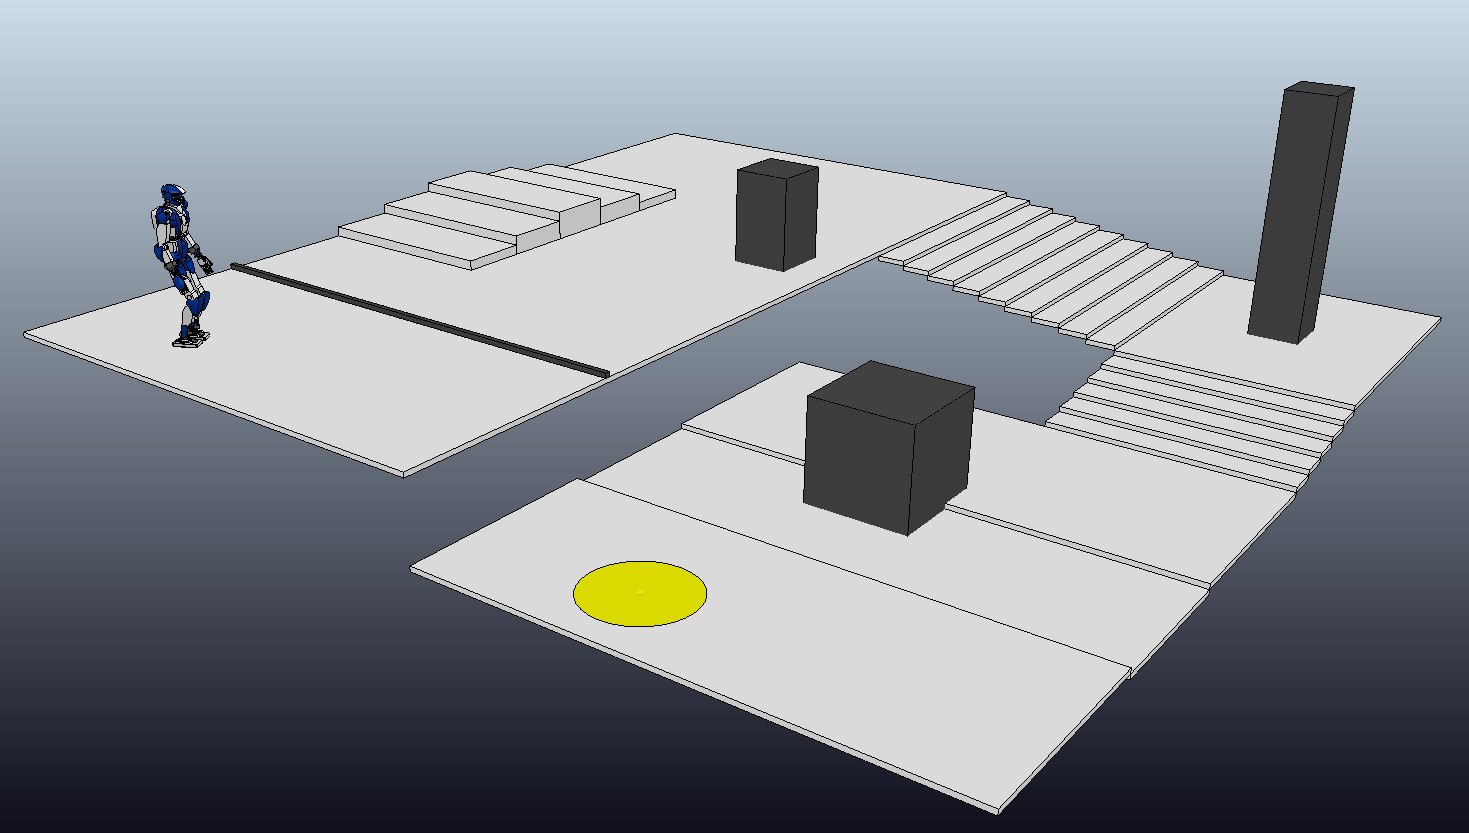
\includegraphics[width=0.9\textwidth]{figures/WoS_Scenario.jpeg}
    \caption{An instance of the considered problem. The robot must reach the
        goal region (in yellow) by traversing a {\em world of stairs}.
        Patches that are not visible correspond to infinitely deep holes or
        trenches.}
    \label{fig:WoS:WoSScenario}
\end{figure}

The mission of the robot is to reach a certain goal region $\cal G$, which will
belong in general to a single patch (Fig.~\ref{fig:WoS:WoSScenario}).
In particular, this locomotion task is accomplished as soon as the robot
places a footstep inside $\cal G$.

We want to devise a complete framework enabling the humanoid to plan and
execute a motion to fulfill the assigned task in the world of stairs.
This requires addressing two fundamental problems: finding a 3D footstep plan
and generating a variable-height gait that is consistent with such plan.
Footstep planning consists in finding both footstep placements and swing foot
trajectories between them; overall, the footstep plan must be feasible
(in a sense to be formally defined later) for the humanoid, given the
characteristics of the environment. Gait generation consists in finding a
CoM trajectory which realizes the footstep plan while guaranteeing dynamic
balance of the robot at all time instants. From the trajectories of the CoM
and the feet, a whole-body motion may be computed using inverse kinematics
methods.

In particular, we will address two versions of the above problem, henceforth
referred to as the \textit{off-line} and \textit{on-line} case. In the first,
the geometry of the environment is completely known in advance, while in the
second it is reconstructed by the robot itself as it moves. 
In the following we describe the architectures designed for the off-line
and on-line case supposing that the environment is static.
However, we will also show that the latter can be used effectively in
dynamic environments, thanks to its fast replanning capabilities. 

The problem will be solved under the following assumptions.

\begin{itemize}

\item[A1] Information about the environment is maintained in an
{\em elevation map} ${\cal M}_{z}$, i.e., a 2.5D grid map of equally-sized
cells that, whenever needed, can be queried as $z = {\cal M}_{z}(x,y)$, to
provide the height of the ground at the cell having coordinates $(x,y)$
\cite{Burgard2016WorldModeling}.
In the off-line case, ${\cal M}_{z}$ is available a priori, while in the
on-line case it must be incrementally built by the humanoid based on sensory
information. 
    
\item[A2] The humanoid is equipped with a head-mounted RGB-D camera, which is
used for localization in both the off-line and on-line cases, and also updating
the elevation map ${\cal M}_{z}$ in the latter.
    
\item[A3] The humanoid is endowed with a localization module which provides an
estimate of the camera pose at each time instant, based on information gathered
by the RGB-D camera. This is used in both the off-line and on-line cases.

\item[A4] The friction between the robot feet and the ground is sufficiently
large to avoid slipping at the contact surfaces\footnote{Since our objective
is to generate walking gaits in a world of stairs, we expect that the horizontal
components of the ground reaction forces will be rather limited with respect
to the vertical components, making this assumption reasonable. Nevertheless,
the constraint that ground reaction forces must always be contained in the
friction cone can be incorporated in our formulation; this extension would be
required in the case of non-horizontal contact surfaces.}.

\end{itemize}

In the off-line case, a complete footstep plan leading to the goal region
$\cal G$ will be computed before the humanoid starts to move. In the
on-line case, the footstep plan will instead be updated during motion, based on
new information added to ${\cal M}_{z}$. 

In the following, we first address in full detail the off-line case and then
proceed to extending the proposed approach to the on-line case.

\section{The off-line case} 
\label{sec:WoS:offlineCase}
We start this section by describing the general structure of the proposed
method. Then we will describe the footsep planner and present some simulations.
The gait generation scheme used is the one presented in Chapter \ref{ch:ISMPC}.

\subsection{General architecture}
\label{sec:WoS:offlineCase:GeneralArchitecture}
To solve the described problem in the off-line case, we adopt the architecture
shown in Fig.~\ref{fig:WoS:blockScheme1}, in which the main components are the
footstep planning, gait generation and localization modules.

\begin{figure}
    \centering
    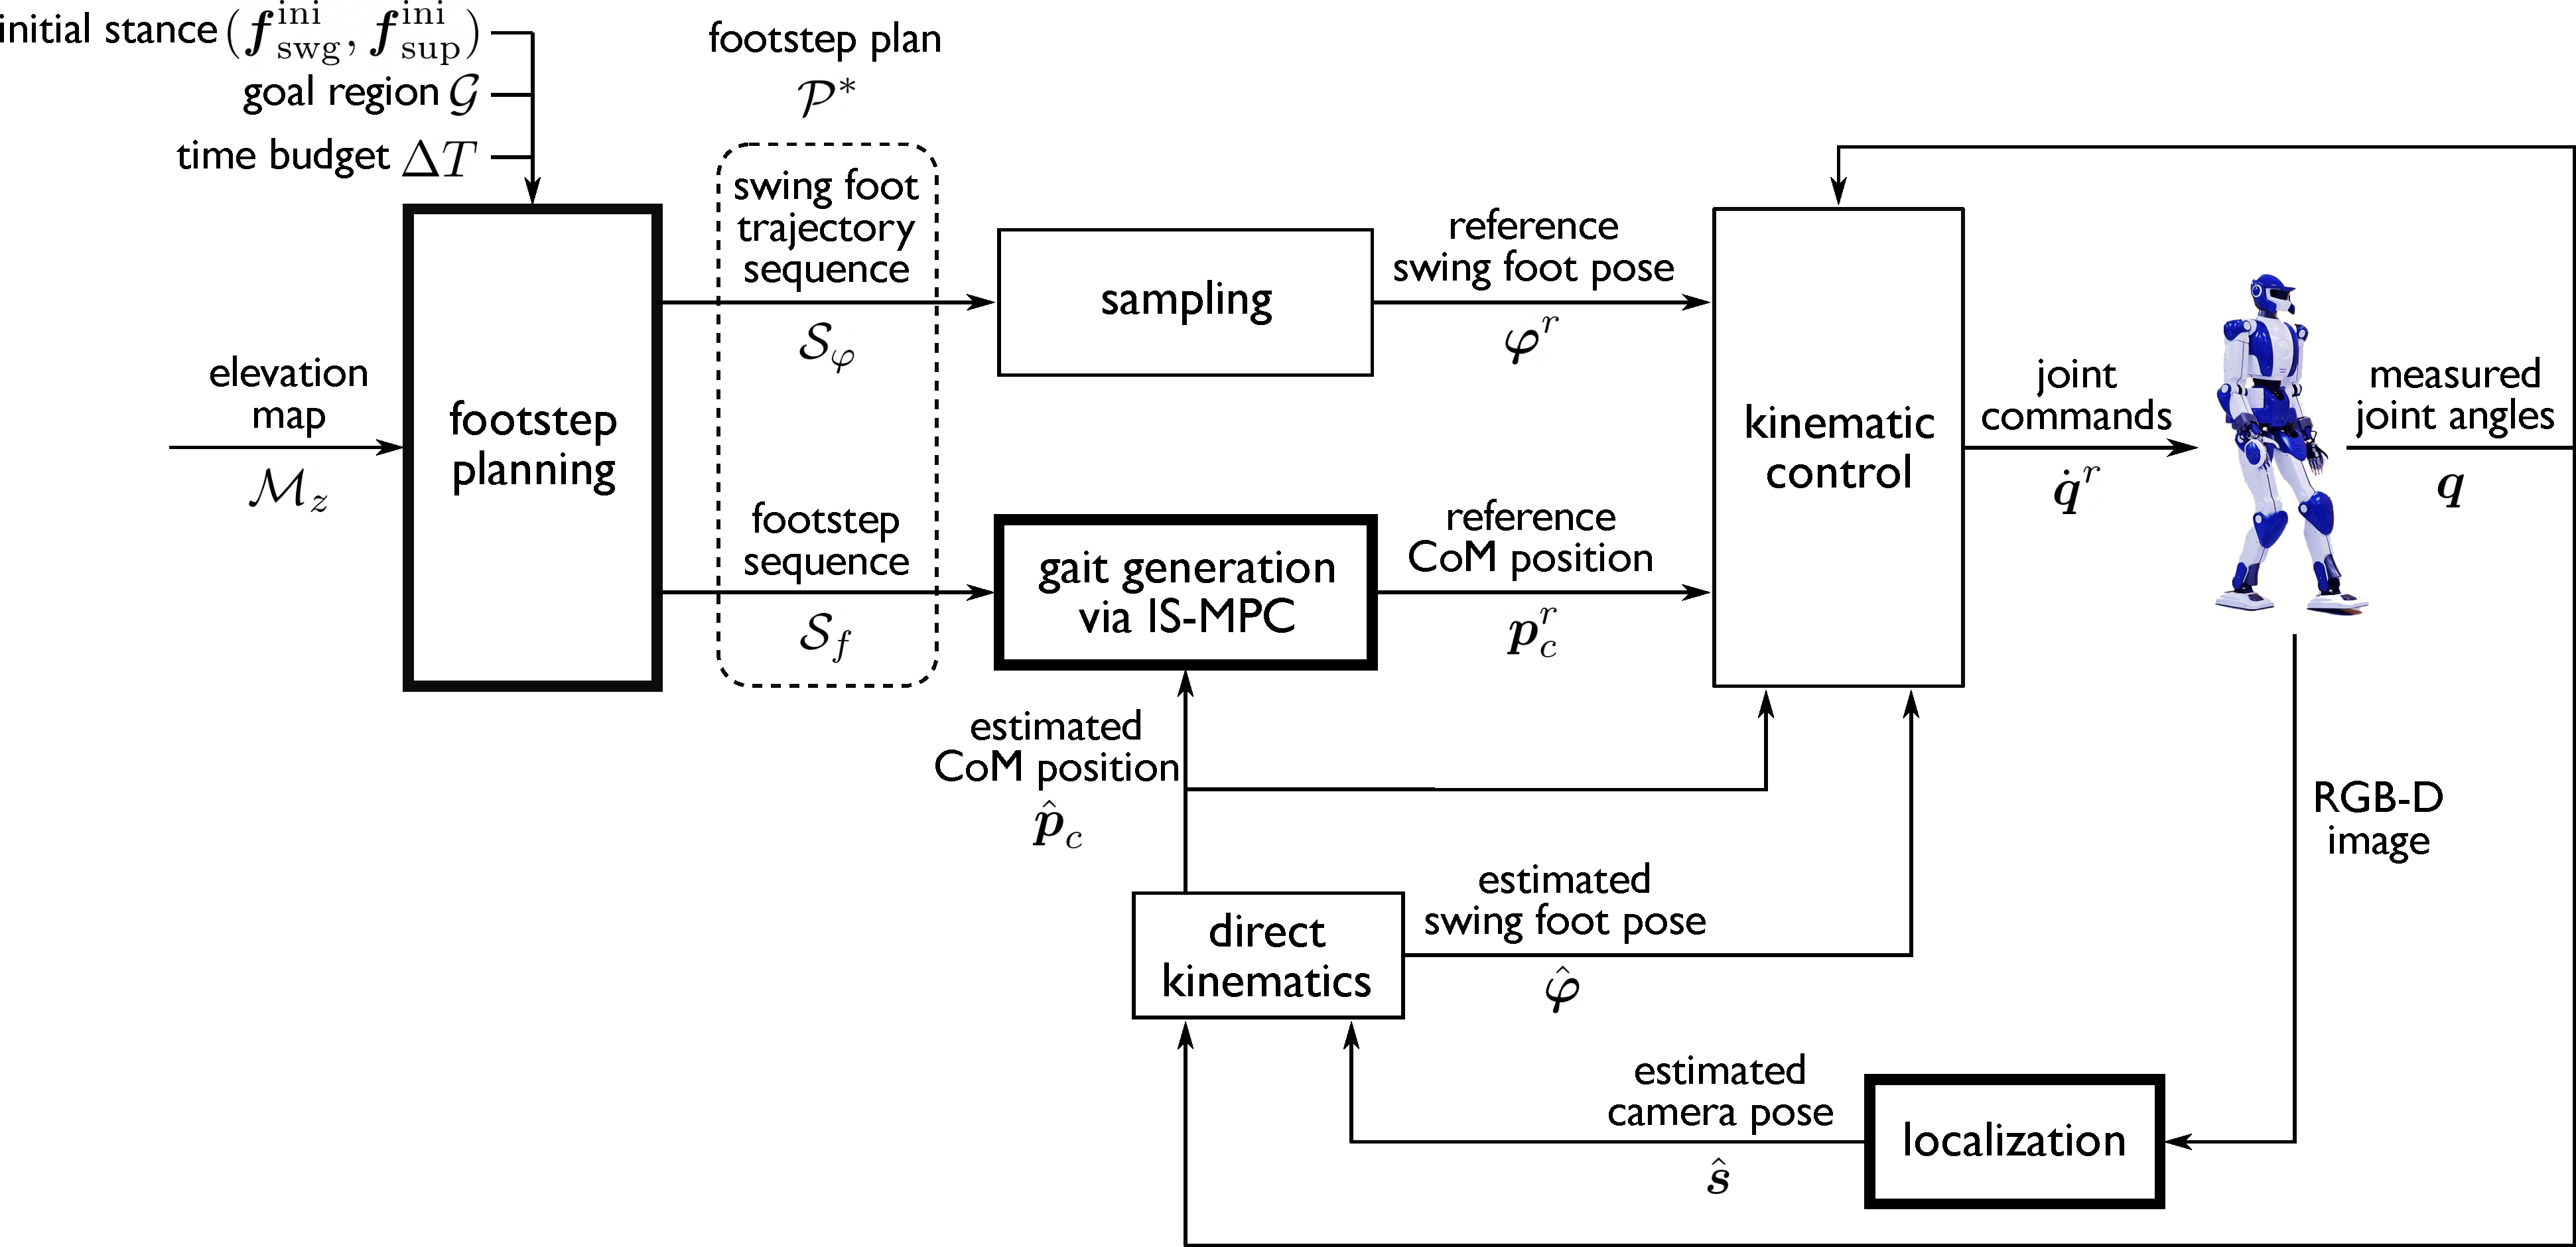
\includegraphics[width=\textwidth]{figures/BlockSchemeOffline.pdf}
    \caption{Block scheme of the proposed solution approach for the off-line case.}
    \label{fig:WoS:blockScheme1}
\end{figure}

In the following, we denote by $\bff = (x_{f}, y_{f}, z_{f}, \theta_{f})$ the
{\em pose} of a certain footstep, with $x_{f}$, $y_{f}$, $z_{f}$ representing
the coordinates of a representative point, henceforth collectively denoted as
$\bfp_f$, and $\theta_{f}$ its orientation\footnote{To represent the footstep
orientation we only use the yaw angle, as roll and pitch are always zero thanks
to the piecewise-horizontal ground assumption.}.
Moreover, a pair $(\bff_{\rm swg}, \bff_{\rm sup})$ defines a {\em stance},
i.e., the feet poses during a double support phase after which a step is
performed by moving the swing foot from $\bff_{\rm swg}$ while keeping the
support foot at $\bff_{\rm sup}$. 

The footstep planner receives in input the initial humanoid
stance\footnote{The initial support foot can be chosen arbitrarily.}
$(\bff_{\rm swg}^{\rm ini}, \bff_{\rm sup}^{\rm ini})$ at $t=0$, the goal
region $\cal G$, a time budget $\Delta T$, and the elevation map ${\cal M}_z$
representing the environment.

The time budget represents the time given to the planner to find a solution.
When this time runs over, the algorithm either returns a solution or ends
with a failure. Explicitly specifying this time as input to the algorithm
allows us to evaluate the performance of the planning module, but also proves
to be useful for the extension to the on-line case, where the time budget is
set equal to the duration of a step in order to meet the real-time requirement.

The planner works off-line to find, within $\Delta T$, an optimal
\textit{footstep plan} ${\cal P}^\ast = \{ {\cal S}_f, {\cal S}_\varphi \}$
leading to the desired goal region $\cal G$. In ${\cal P}^*$, we denote by
\begin{equation*}
    {\cal S}_f = \{\bff^1, \dots, \bff^n\}
\end{equation*}
the sequence of footstep placements, whose generic element $\bff^j$ is the
pose of the $j$-th footstep, with $\bff^1 = \bff_{\rm swg}^{\rm ini}$ and
$\bff^2 = \bff_{\rm sup}^{\rm ini}$. Also, we denote by
\begin{equation*}
    {\cal S}_\varphi = \{\bfvarphi^1, \dots, \bfvarphi^{n-2}\}
\end{equation*} 
the sequence of associated swing foot trajectories, whose generic element
$\bfvarphi^j$ is the $j$-th {\em step}, i.e., the trajectory leading the foot
from $\bff^{j}$ to $\bff^{j+2}$. Its duration $T_s^j$ is split in $T_{\rm ss}^j$
and $T_{\rm ds}^j$, respectively the single and double support phases. 
The timestamp of a generic footstep indicates the beginning of the $j$-th step,
i.e., of the $j$-th single support phase; thus, $\bff^{j}$ has an associated
timestamp $t_s^{j} = t_s^{j-1} + T_s^{j-1}$, with $t_s^{1}=0$.

Once the footstep plan has been generated, the sequence of footsteps
${\cal S}_{f}$ is sent to a gait generator based on IS-MPC
(Chapter \ref{ch:ISMPC}), which computes in real time a variable-height
CoM trajectory that
is compatible with ${\cal S}_{f}$ and guaranteed to be {\em stable} (i.e.,
bounded with respect to the ZMP). In particular, we denote by $\bfp_{\rm c}^r$
the current reference position of the CoM produced by IS-MPC. Also, let
$\bfvarphi^r$ be the current reference pose of the swing foot, obtained by
sampling the appropriate subtrajectory in ${\cal S}_{\varphi}$. Then,
$\bfp_{\rm c}^r$ and $\bfvarphi^r$ are passed to a kinematic controller which
computes the joint commands $\dot{\bfq}^r$ for the robot.

Visual information, gathered by the head-mounted camera in the form of RGB-D
images, is provided to the localization module, which continuously updates the
estimate $\hat{\bfs}$ of the pose of the camera frame.
From this, and using joint encoder data, it is possible to obtain estimates for
the CoM position and swing foot pose ($\hat \bfp_c$ and $\hat \bfvarphi$,
respectively) through kinematic computations. Finally, these estimates are used
to provide feedback to both the gait generation and kinematic control modules.

\subsection{Footstep planning}
\label{sec:WoS:offlineCase:FootstepPlanner}

The input data for this module are the initial robot stance
$(\bff_{\rm swg}^{\rm ini}, \bff_{\rm sup}^{\rm ini})$, the goal region
$\cal G$, the time budget $\Delta T$ and the elevation map ${\cal M}_z$.
Given an optimality criterion, the footstep planner returns the best footstep
plan ${\cal P}^*$ leading to $\cal G$ found within $\Delta T$. 

The planning algorithm builds a tree $\cal T$, where each vertex
$v = (\bff_{\rm swg}, \bff_{\rm sup})$ specifies a stance, and an edge between
two vertexes $v$ and $v' = (\bff'_{\rm swg}\!=\!\bff_{\rm sup}, \bff'_{\rm sup})$
indicates a step between the two stances, i.e., a collision-free trajectory such
that one foot swings from $\bff_{\rm swg}$ to $\bff'_{\rm sup}$ and the other
is fixed at $\bff_{\rm sup}$.

The expansion process makes use of a catalogue $U$ of {\em primitives}, which
allows to generate new footsteps by selecting them from a finite set of
displacements with respect to the support foot. The catalogue is split in two
subsets, one for the case of left support  and the other for the case of right
support; at each instant, the appropriate subset is used. An example catalogue
is shown in Fig.~\ref{fig:WoS:Primitives}.

\begin{figure}
    \centering
    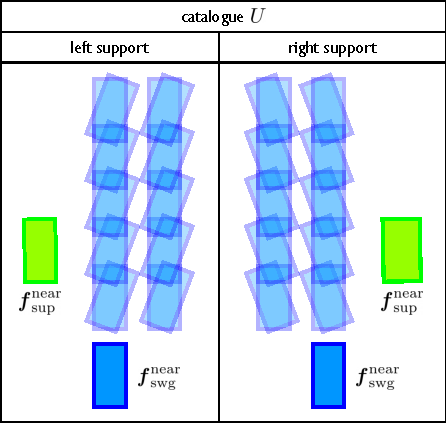
\includegraphics[width=0.65\textwidth]{figures/Primitives.pdf}
    \caption{An example catalogue $U$ of primitives, containing a finite set of
    landings for the swing foot with respect to the left or right support foot.}
    \label{fig:WoS:Primitives}
\end{figure}

Each branch joining the root of the tree to a generic vertex $v$ represents a
footstep plan $\cal P$. The sequences ${\cal S}_f$ and ${\cal S}_\varphi$ for
this plan are respectively obtained by taking along the branch the support foot
poses of all vertexes and the steps corresponding to all edges.

\medskip

\subsubsection{Footstep feasibility}
Footstep $\bff^j=(x_f^j,y_f^j,z_f^j,\theta_f^j) \in {\cal S}_f$ is
\textit{feasible} if it satisfies the following requirements:   

\begin{itemize}

\smallskip
\item[R1] $\bff^j$ is fully in contact within a single horizontal patch.

\smallskip
To guarantee this, each cell of ${\cal M}_{z}$ belonging to, or overlapping
with, the footprint at $\bff^j$ must have the same height $z_{f}^j$.
In practice, one typically uses an enlarged footprint to ensure that this
requirement will still be satisfied in the presence of small positioning errors.

\smallskip
% this is actually stance feasibility 
\item[R2] $\bff^j$ is kinematically admissible from the previous footstep
$\bff^{j-1}$ (this is actually {\em stance feasibility}).

\smallskip
%The admissible region (a submanifold of $\RealSet^3 \times SO(2)$) for placing $\bff^{j}$ next to $\bff^{j-1}$ is denoted by ${\cal A}(\bff^{j-1})$ and is defined by the following constraints:
The admissible region (a submanifold of $\RealSet^3 \times SO(2)$) for placing
$\bff^{j}$ next to $\bff^{j-1}$ is defined by the following constraints:
\begin{gather} 
-\begin{pmatrix}
\Delta_x^- \\[5pt] \Delta_y^-
\end{pmatrix}
\le
R_{j-1}^T \begin{pmatrix}
x_f^j - x_f^{j-1} \\[5pt] y_f^j - y_f^{j-1}
\end{pmatrix}
\pm \begin{pmatrix}
0 \\ \ell
\end{pmatrix}
\le
\begin{pmatrix}
\Delta_x^+ \\[5pt] \Delta_y^+
\end{pmatrix} \label{eq:WoS:XYAdmissible}\\[5pt]
-\Delta_z^- \le z_f^j - z_f^{j-1} \le \Delta_z^+
\label{eq:WoS:ZAdmissible}\\[5pt]
-\Delta_\theta^- \le \theta_f^j - \theta_f^{j-1} \le \Delta_\theta^+. \label{eq:WoS:ThetaAdmissible}
\end{gather}
Here, $R_{j-1}$ is the planar rotation matrix associated with $\theta_f^{j-1}$
and the $\Delta$ symbols are lower and upper maximum increments, see
Fig.~\ref{fig:WoS:KinCon}.

\begin{figure}
\centering
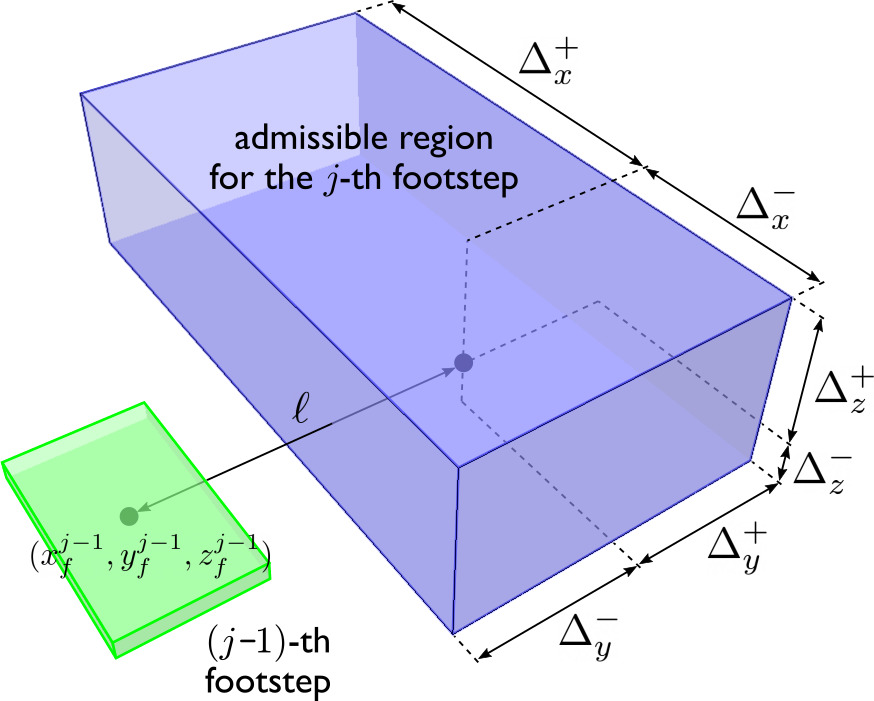
\includegraphics[width=0.6\textwidth]{figures/kinematic_limits.jpeg}
\caption{The 3D admissible region identified by the first two kinematic
constraints of requirement R2, i.e.,
eqs. (\ref{eq:WoS:XYAdmissible}-- \ref{eq:WoS:ZAdmissible}).
Footstep orientation is not represented.}
\label{fig:WoS:KinCon}
\end{figure}

% this is actually step feasibility, i.e., compatibility between successive stances
\smallskip
\item[R3] $\bff^j$ is reachable from $\bff^{j-2}$ through a collision-free
motion (this is actually {\em step feasibility}).

\smallskip
Since information about the whole-body motion of the robot is not yet available
during footstep planning (it will only be defined in the subsequent gait
generation phase), this requirement can only be tested conservatively.
In particular, we say that R3 is satisfied if ({\em i}) there exist a
collision-free swing foot trajectory $\bfvarphi^{j-2}$ from $\bff^{j-2}$ to
$\bff^{j}$ generated by the engine of
Sect.~\ref{sec:WoS:offlineCase:FP:PlannerOverview}, and ({\em ii}) a suitable
volume ${\cal B}$ accounting for the maximum occupancy of the humanoid upper
body at stance $(\bff^{j-1}, \bff^{j})$ is collision-free. More precisely,
${\cal B}$ is a vertical cylinder whose base has radius $r_b$ and center at
$(x_m, y_m, z_m + z_b)$, where $x_m$, $y_m$, $z_m$ are the coordinates of the
midpoint $\bfm$ between the footsteps and $z_b$ is a vertical offset
representing the average distance between the ground and the hip
(Fig. \ref{fig:WoS:ReqCollisionCheck}). 
Note that any nonzero height can be used for the cylinder in view of the world
of stairs assumption, which implies that ${\cal B}$ is collision-free
\footnote{Even though the volume for checking the upper body collision is chosen
conservatively, this does not guarantee obstacle avoidance because the lower
body is not considered. However, whole-body collision avoidance can be obtained
by including appropriate constraints in the kinematic controller
\cite{Escande2014IJRR}.} if each cell of ${\cal M}_z$ belonging to, or
overlapping with, its ground projection has height smaller than $z_m + z_b$.

\end{itemize}

\medskip

\subsubsection{Vertex identity, neighbors and cost}
\label{sec:WoS:offlineCase:FP:CostFunctions}
The {\em identity} of a vertex $v=(\bff_{\rm swg}, \bff_{\rm sup})$ indicates
whether  $\bff_{\rm swg}$ refers to the left ($L$) or the right ($R$) foot:
\[
{\rm id}(v)=
\begin{cases}
L\quad \mbox{if} \quad{\rm id}(v^{\rm parent}) = R \\
R\quad \mbox{if} \quad{\rm id}(v^{\rm parent}) = L,
\end{cases}
\]
where $v^{\rm parent}$ is the parent vertex of $v$.
This definition determines the identity of each vertex, once the identity of
the root is assigned.

We also define the set of {\em neighbors} of $v=(\bff_{\rm swg}, \bff_{\rm sup})$
\[
{\cal N}(v) = \{ v'=(\bff'_{\rm swg}, \bff'_{\rm sup}) \in {\cal T} : 
 \gamma(\bff_{\rm sup}, \bff'_{\rm sup}) \le r_{\rm neigh}\}
\]
where $r_{\rm neigh}$ is a threshold distance and
\begin{equation}
\gamma(\bff, \bff') = \lVert \bfp_f - \bfp_f' \rVert + k_{\gamma}|\theta_f-\theta_f'|
\label{eq:WoS:footstepToFootstepMetric}
\end{equation}
is a footstep-to-footstep metric, with $k_{\gamma}\ge 0$.

\begin{figure}
\centering
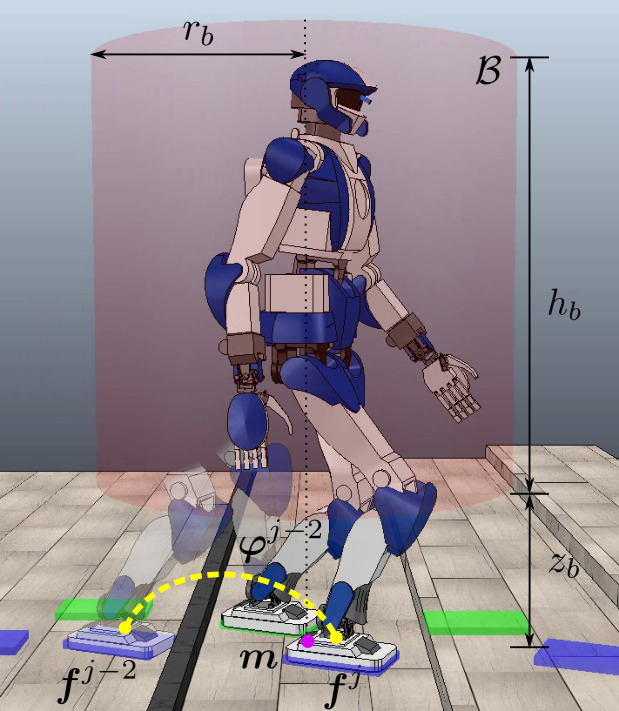
\includegraphics[width=0.55\textwidth]{figures/R3_CollisionCheck.jpeg}
\caption{Visual representation of the process for checking requirement R3.
The red cylinder accounts for the maximum occupancy of the humanoid upper body,
while the yellow line represents the swing foot trajectory.}
\label{fig:WoS:ReqCollisionCheck}
\end{figure}

Assume that the edge between two vertexes $v^a$ and $v^b$ of $\cal T$ has a
cost $l(v^a,v^b)$. 
The {\em cost} of a vertex $v$ is defined as
\[
c(v) = c(v^{\rm parent}) + l(v^{\rm parent}, v)
\]
and represents the cost of reaching $v$ from the root of $\cal T$. 
Then, the cost of a plan $\cal P$ ending at a vertex $v$ is $c({\cal P}) = c(v)$.

In particular, we will consider three possibilities for the cost of an edge.
The first is
\begin{equation}
l_1(v^a, v^b) = 1,
\label{eq:WoS:costSteps}
\end{equation}
for all edges in $\cal T$. The corresponding vertex cost will be denoted by
$c_1(v)$ and represents the length of the corresponding plan in terms of number
of edges (i.e., steps). 
    
\begin{figure}
\centering
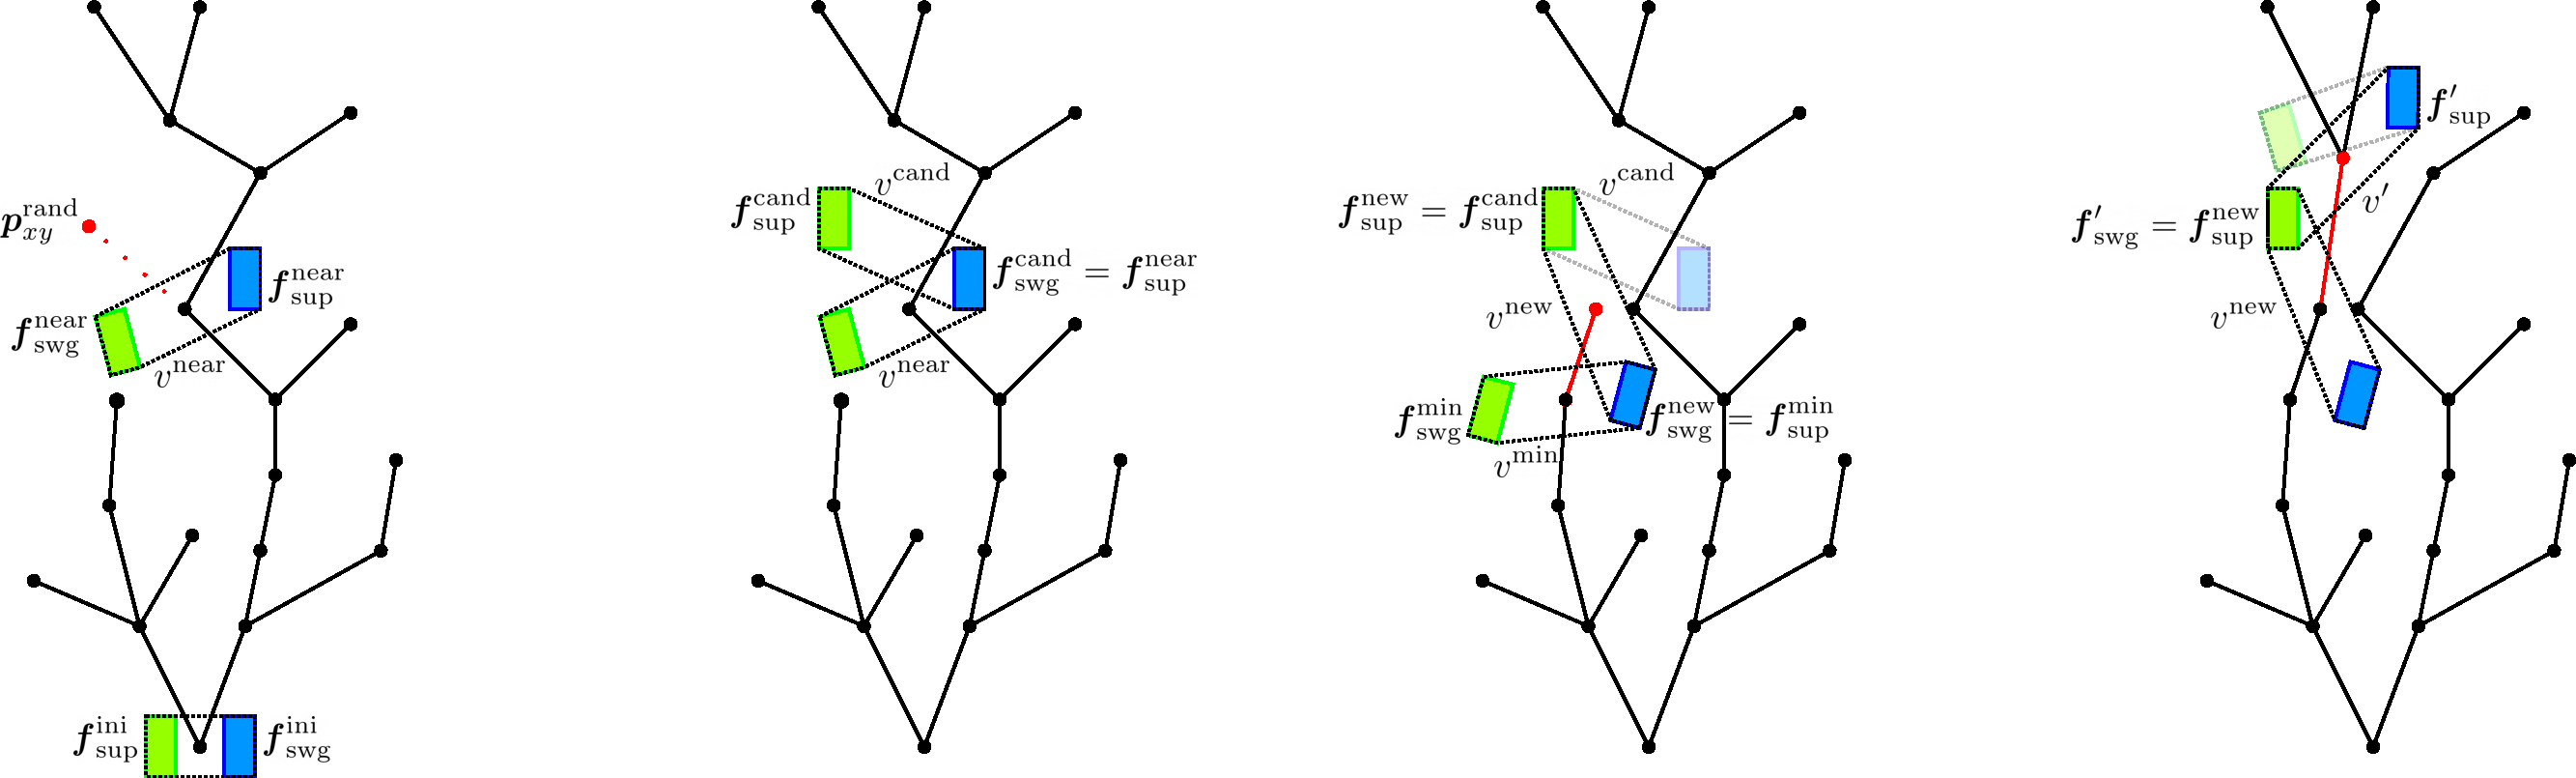
\includegraphics[width=\textwidth]{figures/FootstepPlanner.pdf}
\caption{The four steps of a generic iteration of the footstep planner.
First, a sampled point is used to select a vertex for expansion.
Then, the selected vertex is used to generate a candidate vertex to be inserted
in the tree.
In the third step, a parent for the candidate vertex is chosen.
Finally, a rewiring procedure is called to update the tree, guaranteeing that
the cost of the nodes is optimal.}
\label{fig:WoS:FootstepPlanner}
\end{figure}   
    
The second edge cost represents the net height variation of the swing foot
during a step:
\begin{equation}
l_2(v^a, v^b) = |z^b_{f, {\rm sup}} - z^a_{f, {\rm swg}}|,
\label{eq:WoS:costHeight}
\end{equation}
where $z^a_{f, {\rm swg}}$ and $z^b_{f, {\rm sup}}$ are the $z$-component of,
respectively, the swing foot at $v^a$ and the support foot at $v^b$.
The corresponding vertex cost will be denoted by $c_2(v)$ and represents the
cumulative height variation along the corresponding plan. 
    
Finally, we  also consider as edge cost
\begin{equation}
l_3(v^a, v^b) = \frac{1}{\sigma (\bff^b_{\rm sup})},
\label{eq:WoS:costClearance}
\end{equation}
where $\sigma (\bff^b_{\rm sup})$ is the {\em clearance} of the support foot
$\bff^b_{\rm sup}$ at $v^b$, defined as the distance between the representative
point of $\bff^b_{\rm sup}$ and the closest point in $\mathcal{M}_z$
w.r.t. which the absolute height variation is larger than
$\max\{\Delta_z^-, \Delta_z^+\}$\footnote{This information may be precomputed
from the elevation map ${\cal M}_z$ and stored in a clearance map.}.
This cost penalizes steps that bring the swing foot too close to a drop or to
a vertical surface leading to a contiguous higher patch,
while still allowing to approach accessible patches such as staircases.
The corresponding vertex cost, denoted by $c_3(v)$, represents the cumulative
inverse clearance along the corresponding plan.

Other kinds of cost functions can be considered. For example, one could penalize
unnecessary rotations of the next footstep with respect to the support footstep
in order to obtain smoother plans.  
In general, it may be advisable to use a weighted combination of several
optimality criteria for better practical performance. 

\medskip

\subsubsection{Algorithm}
\label{sec:WoS:offlineCase:FP:PlannerOverview}

We now describe the footstep planning algorithm for the off-line case
(Algorithm \ref{alg:FootstepPlanner}).

At the beginning, $\cal T$ is rooted at
$(\bff_{\rm swg}^{\rm ini}, \bff_{\rm sup}^{\rm ini})$, the initial stance of
the humanoid.
Then, $\cal T$ is expanded using an RRT*-like strategy. The generic iteration
consists of: selecting a vertex for expansion, generating a candidate vertex,
choosing a parent for the new vertex and rewiring the tree. These individual
steps are described in the following, see also Fig.~\ref{fig:WoS:FootstepPlanner}.

\begin{algorithm}%[!t]
	\small
	\removelatexerror
    %\caption{FootstepPlanner$(({\bff}_{\rm swg}^{\rm ini}, {\bff}_{\rm sup}^{\rm ini}), {\cal G}, {\Delta T}, {\cal M}_z)$}
	
	\caption{FootstepPlanner}
	\label{alg:FootstepPlanner}

	\KwIn{$({\bff}_{\rm swg}^{\rm ini}, {\bff}_{\rm sup}^{\rm ini}), {\cal G}, {\Delta T}, {\cal M}_z$}
	\vspace{2pt}
	\KwOut{${\cal P}^*$}
    \BlankLine
    
	$v^{\rm ini}$ $\leftarrow$ $({\bff}_{\rm swg}^{\rm ini}$, ${\bff}_{\rm sup}^{\rm ini})$\; 
	
	AddVertex$(\cal T$, $\emptyset$, $v^{\rm ini}$, $\emptyset)$\;
	
	ExpandTree$(\cal T$, ${\Delta T}$, ${\cal M}_z)$\;
	
    ${\cal P}^*$ $\leftarrow$ RetrieveBestPlan$({\cal T}, {\cal G})$\;	
    \Return{${\cal P}^*$}\;
\end{algorithm}

\begin{procedure}%[!t]
	\small
	\removelatexerror
	%\caption{ExpandTree(${\cal T}$, ${\Delta T}$, ${\cal M}_z$)}
	
	\caption{ExpandTree()}
	\label{proc:ExpandTree}

	\KwIn{${\cal T}, {\Delta T}, {\cal M}_z$}
	\vspace{2pt}
	\KwOut{none}
    \BlankLine
    
	\While{\rm \textbf{not} TimeExpired$({\Delta T})$}{
	 	$\bfp_{xy}^{\rm rand}$ $\leftarrow$ SamplePoint$()$\;
	 	$v^{\rm near}$ $\leftarrow$ NearestVertex$(\mathcal{T}, \bfp_{xy}^{\rm rand})$\;
	 	$\bff^{\rm cand}_{\rm sup}$ $\leftarrow$ GenerateCandidateFootstep$(\bff_{\rm sup}^{\rm near}, U, \mathcal{M}_z)$\;
	 	
	 	\If{\rm R1$(\bff^{\rm cand}_{\rm sup})$ \rm \textbf{and} \rm R2$(\bff^{\rm cand}_{\rm sup}, \bff^{\rm near}_{\rm sup})$}{
	 	 	$\bfvarphi^{\rm near}$ $\leftarrow$ SwingTrajectoryEngine$(\bff_{\rm swg}^{\rm near}, \bff_{\rm sup}^{\rm cand})$\;
		 	
		 	\If{\rm R3$(\bfvarphi^{\rm near}, (\bff^{\rm near}_{\rm sup}, \bff^{\rm cand}_{\rm sup}))$}{
		 	    $v^{\rm cand}$ $\leftarrow (\bff^{\rm near}_{\rm sup}, \bff^{\rm cand}_{\rm sup})$\;
		 		
		 		$\mathcal{N} \leftarrow$ Neighbors$(\mathcal{T}, v^{\rm cand})$\;
		 		
		 		$(v^{\rm min}, \bfvarphi^{\rm min}) \leftarrow$ ChooseParent$(\mathcal{T}, \mathcal{N}, v^{\rm near}, v^{\rm cand}, \bfvarphi^{\rm near})$\;
		 		
                $v^{\rm new} \leftarrow (\bff^{\rm min}_{\rm sup}, \bff^{\rm cand}_{\rm sup})$\;
		 		
		 		AddVertex$(\mathcal{T}, v^{\rm min}, v^{\rm new}, \bfvarphi^{\rm min})$\;	
		 		
		 		ReWire$(\mathcal{T}, \mathcal{N}, v^{\rm new})$\;	
		 	}   			
	 	}    
	 }
	 \Return{}\;
\end{procedure}

{\bf Selecting a vertex for expansion}: A point $\bfp_{xy}^{\rm rand}$ is
randomly selected on the $xy$-plane, and
the vertex $v^{\rm near}$ that is closest to $\bfp_{xy}^{\rm rand}$ is
identified. To this end, we define a vertex-to-point metric as
\begin{equation*}
\mu(v, \bfp_{xy}) = \lVert \bfm_{xy}(v) - \bfp_{xy} \rVert + k_{\mu} |\psi(v,\bfp_{xy})|,
\end{equation*}
where $\bfm_{xy}(v)$ represents the planar position of the midpoint between the
feet at stance $v$, $k_{\mu}$ is a positive scalar, and $\psi(v,\bfp_{xy})$ is
the angle between the robot sagittal axis (whose orientation is the average of
the orientations of the two footsteps) and the line joining $\bfm_{xy}$ to
$\bfp_{xy}$. This step corresponds to the functions SamplePoint and
NearestVertex in Procedure \ref{proc:ExpandTree}.
\hfill $\blacktriangleleft$

\begin{sloppypar}
{\bf Generating a candidate vertex}:  
After identifying the vertex
${v^{\rm near}=(\bff_{\rm swg}^{\rm near},\bff_{\rm sup}^{\rm near})}$,
a candidate footstep is first generated using the catalogue $U$
(see Fig.~\ref{fig:WoS:Primitives}). In particular, we set the support foot to
$\bff_{\rm sup}^{\rm near}$ and randomly select one element from the subset of
$U$ associated to the identity of $v^{\rm near}$, which may be $L$ (left) or
$R$ (right). Note that all elements of $U$ are chosen so as to automatically
satisfy conditions~(\ref{eq:WoS:XYAdmissible}--\ref{eq:WoS:ThetaAdmissible})
of requirement R2. Call $\bff_{\rm sup}^{\rm cand}$ the chosen candidate
footstep. The $z$ coordinate to be associated to the footstep
$\bff_{\rm sup}^{\rm cand}$ is then retrieved from ${\cal M}_{z}$, and both
the requirement R1 and the last condition~(\ref{eq:WoS:ZAdmissible}) of R2 can
now be checked.
\end{sloppypar}

To test the last requirement R3, we invoke an engine
(Procedure \ref{proc:genswgtraj}) that generates a swing foot trajectory
$\bfvarphi^{\rm near}$ from $\bff_{\rm swg}^{\rm near}$ to
$\bff_{\rm sup}^{\rm cand}$. Such engine uses a parameterized trajectory which,
given the endpoints, can be deformed\footnote{As a deformable trajectory we
used a polynomial, but other choices (e.g., B-splines and Bezier curves) are
possible.} by varying the maximum height $h$ along the motion. 
Using the elevation map and increments of $\Delta h$, the engine tries growing
values of $h$ in a certain range $[h^{\rm min}, h^{\rm max}]$ looking for a
collision-free trajectory.

If all requirements have been satisfied, a candidate vertex is generated as
$v^{\rm cand} = (\bff_{\rm swg}^{\rm cand}, \bff_{\rm sup}^{\rm cand})$, with
$\bff_{\rm swg}^{\rm cand} = \bff_{\rm sup}^{\rm near}$; however, $v^{\rm cand}$
is not added to $\cal T$ because the planner first needs to identify the best
parent for it. If any requirement among R1--R3 is violated, the current
expansion attempt is aborted and a new iteration is started.
This step corresponds to lines 4-8 in Procedure \ref{proc:ExpandTree}.
\hfill $\blacktriangleleft$

\begin{procedure}%[!t]
	\small
	\removelatexerror
	
	%\caption{SwingTrajectoryEngine($\bff^a$, $\bff^b$)}
	\caption{SwingTrajectoryEngine()}
	\label{proc:genswgtraj}

	\KwIn{$\bff^a$, $\bff^b$}
	\KwOut{$\bfvarphi^a$}
    \BlankLine

	$h$ $\leftarrow$ $h^{\rm min}$\;
	
	\While{$h \leq h^{\rm max}$}{
		$\bfvarphi^a \leftarrow$ DeformTrajectory$(\bff^a, \bff^b, h)$\;		 	
	
	   	\If{\rm CollisionFree$(\bfvarphi^a)$}{
            \Return{$\bfvarphi^a$}\;	   	
	   	}
		
	    $h \leftarrow h + \Delta h$\;
	}
			
	\Return{$\emptyset$}\;	
\end{procedure}

{\bf Choosing a parent}: Although $v^{\rm cand}$ was generated from
$v^{\rm near}$, there might be a different vertex in the tree that leads to
the same vertex with a lower cost. To find it, the planner checks for each
vertex $v' = (\bff'_{\rm swg}, \bff'_{\rm sup})\in {\cal N} (v^{\rm cand})$
whether setting $v'$ as parent of $v^{\rm cand}$ satisfies requirements R2-R3,
and whether this connection reduces the cost of $v^{\rm cand}$, that is 
\[
c(v') + l(v', v^{\rm cand}) < c(v^{\rm near}) + l(v^{\rm near}, v^{\rm cand}).
\]
The vertex $v^{\rm min} = (\bff_{\rm swg}^{\rm min}, \bff_{\rm sup}^{\rm min})$
that allows to reach $v^{\rm cand}$ with minimum cost is chosen as its parent.
If $v^{\rm min} = v^{\rm near}$, then $v^{\rm cand}$ can be added to the tree
together with the edge joining it to $v^{\rm near}$. However, if a different
parent $v^{\rm min} \neq v^{\rm near}$ is chosen, the candidate vertex
$v^{\rm cand}$ must be modified by relocating its swing footstep to the support
footstep of $v^{\rm min}$. To this end, a new vertex
$v^{\rm new} = (\bff_{\rm swg}^{\rm new}, \bff_{\rm sup}^{\rm new})$ with
$\bff_{\rm swg}^{\rm new} = \bff_{\rm sup}^{\rm min}$ and
$\bff_{\rm sup}^{\rm new} = \bff_{\rm sup}^{\rm cand}$ is generated and added
to ${\cal T}$ as child of $v^{\rm min}$. The edge between $v^{\rm min}$ and
$v^{\rm new}$ corresponds to the swing foot trajectory $\bfvarphi^{\rm min}$. 
This step corresponds to the function ChooseParent in Procedure
\ref{proc:chooseparent}.
\hfill $\blacktriangleleft$

\begin{procedure}%[!t]
	\small
	\removelatexerror
	%\caption{ChooseParent($\cal T$, $\cal N$, $v^{\rm near}$, $v^{\rm cand}$, $\bfvarphi^{\rm cand}$)}
	
	\caption{ChooseParent()}
	\label{proc:chooseparent}

	\KwIn{${\cal T}, {\cal N}, v^{\rm near}, v^{\rm cand}, \bfvarphi^{\rm cand}$}
	\vspace{2pt}
	\KwOut{$v^{\rm min}, \bfvarphi^{\rm min}$}
    \BlankLine
	
	$v^{\rm min}$ $\leftarrow$ $v^{\rm near}$\;
	$\bfvarphi^{\rm min}$ $\leftarrow$ $\bfvarphi^{\rm cand}$\;
	$c^{\rm min}$ $\leftarrow$ $c(v^{\rm near}) + l(v^{\rm near}, v^{\rm cand})$\;
	
	\ForEach{$v'$ $\in$ $\cal N$}{
    	\If{\rm R2$(\bff_{\rm sup}^{\rm cand}, \bff'_{\rm sup})$}{
    		$\bfvarphi' \leftarrow$ SwingTrajectoryEngine$(\bff'_{\rm swg}, \bff_{\rm sup}^{\rm cand})$\;
    		
    		\If{\rm R3$(\bfvarphi', (\bff'_{\rm sup}, \bff_{\rm sup}^{\rm cand}))$ \rm \textbf{and} $c(v') +l(v', v^{\rm cand}) < c^{\rm min}$}{
				$v^{\rm min}$ $\leftarrow$ $v'$\;
				$\bfvarphi^{\rm min}$ $\leftarrow$ $\bfvarphi'$\;
				$c^{\rm min}$ $\leftarrow$ $c(v') +l(v', v^{\rm cand})$\;
    		}
    	}
	}
	\Return{$(v^{\rm min}$, $\bfvarphi^{\rm min})$}\;	
\end{procedure}

{\bf Rewiring}: This final step checks whether $v^{\rm new}$ allows to reach
with a lower cost some vertex already in $\cal T$, and updates the tree
accordingly. In particular, for each
$v' = (\bff'_{\rm swg}, \bff'_{\rm sup}) \in {\cal N} (v^{\rm new})$,
the procedure checks whether setting $v'$ as a child of $v^{\rm new}$ satisfies
requirements R2-R3, and whether this connection reduces the cost of $v'$,
that is 
\[
c(v^{\rm new}) + l(v^{\rm new}, v') < c(v').
\]
If this is the case, $v'$ is modified (similarly to what was done when choosing
a parent) by relocating its swing footstep to $\bff_{\rm sup}^{\rm new}$, and
then  reconnected to $\cal T$ as a child of $v_{\rm new}$. The edge between
$v^{\rm new}$ and $v'$ corresponds to the swing foot trajectory
$\bfvarphi^{\rm new}$. Finally, for each child
$v'' = (\bff''_{\rm swg}, \bff''_{\rm sup})$ of $v'$, the swing foot trajectory
$\bfvarphi'$ from the relocated $\bff'_{\rm swg}$ to $\bff''_{\rm sup}$ is
generated and the edge between $v'$ and $v''$ is accordingly
updated\footnote{In case the engine fails to find such trajectory, the subtree
rooted at vertex $v''$ (including $v''$ itself) is simply removed from $\cal T$.}.
This step corresponds to the function ReWire in Procedure \ref{proc:rewire}.

Note that, although ${\cal N} (v^{\rm new})$ can contain ancestors of
$v^{\rm new}$, no cycle will be generated by rewiring.
In fact, it can be easily shown that any ancestor of $v^{\rm new}$ will have a
cost lower or equal than $c(v^{\rm new})$, so that it will never be set as
its child.
\hfill $\blacktriangleleft$

\begin{procedure}%[!t]
	\small
	\removelatexerror
	%\caption{ReWire($\cal T$, $\cal N$, $v^{\rm new}$)}
    \caption{ReWire()}
	\label{proc:rewire}

	\KwIn{${\cal T}, {\cal N}, v^{\rm new}$}
	\vspace{2pt}
	\KwOut{none}
    \BlankLine
			
	\ForEach{$v'$ $\in$ $\cal N$}{
        \If{\rm R2$(\bff'_{\rm sup}, \bff^{\rm new}_{\rm sup})$}{
 	 	
 	 	    $\bfvarphi^{\rm new} \leftarrow$ SwingTrajectoryEngine$(\bff_{\rm swg}^{\rm new}, \bff'_{\rm sup})$\;
	 	
    	 	\If{\rm $R3(\bfvarphi^{\rm new}, (\bff'_{\rm swg}, \bff'_{\rm sup}))$ \textbf{and} $c(v^{\rm new}) + l(v^{\rm new}, v') < c(v')$}{
                
                UpdateVertex$({\cal T}, v', (\bff_{\rm sup}^{\rm new}, \bff'_{\rm sup}))$\;
                
                UpdateEdge$({\cal T}, v^{\rm new}, v', \bfvarphi^{\rm new})$\;
                
                ${\cal V}_{\rm child} \leftarrow$ ChildVertexes$({\cal T}, v')$\;
                
                \ForEach{$v''$ $\in$ ${\cal V}_{\rm child}$}{
                    $\bfvarphi'$ $\leftarrow$ SwingTrajectoryEngine$(\bff'_{\rm swg}, \bff''_{\rm sup})$\;
                    
                    \eIf{$\bfvarphi' \neq \emptyset$}{
                        UpdateEdge$({\cal T}, v', v'', \bfvarphi')$\;
                    }
                    {
                        RemoveSubtree$({\cal T}, v'')$\; 	
                    }
    	 	    }
                 	   
    	 	}
 	    }
	}
		
	\Return\;	

\end{procedure}

\smallskip
%%%% UP TO HERE 

When the assigned time budget ${\Delta T}$ runs out, tree expansion is stopped.
The set ${\cal V}_{\rm goal}$ of vertexes $v$ such that
$\bfp_{f,{\rm sup}} \in {\cal G}$ is retrieved.
The vertex $v^*$ with minimum cost is selected as
\begin{equation}
    \label{eq:WoS:BestVertex}
    v^* = \underset{v \in {\cal V}_{\rm goal}}{\arg\!\min} \ c(v)
\end{equation}
and the corresponding footstep plan ${\cal P}^*$ is retrieved from the branch
of $\cal T$ joining the root to $v^*$.

Clearly, the larger the time budget, the better the quality of the obtained
footstep plan. %(i.e., the planner asymptotically converges to the optimal solution as the number of iterations increases).
We conjecture that our planner inherits the asymptotic optimality property of
the general RRT* algorithm \cite{Karaman2011IJRR}, although we do not have a
formal proof yet.

\subsubsection{Planning results}
\label{sec:WoS:offlineCase:FP:PlanningResults}

To assess the performance of the proposed footstep planner, we performed a
campaign of planning experiments through our C++ implementation on an Intel
Core i7-8700K CPU running at 3.7~GHz.
The tree constructed by the planner is stored in a k-d tree structure
\cite{Yershova2007ImprovingMotionPlanning}, which allows to efficiently perform
search and insertion operations.
The used robot is HRP-4, a 1.5~m tall humanoid with 34 degrees of freedom
by Kawada Robotics.

We considered the five different scenarios (see Fig. \ref{fig:WoS:Scenarios})
of different complexity described in the following.
\begin{itemize}
    \item \textit{Rod}. A thin straight obstacle, which does not provide a large enough surface to step on, must be overcome before ascending and descending a staircase. 
    \item \textit{Ditch}. A ditch can only be entered from the left and exited from the right, because the platform in the middle of it is too low to be accessed directly.
    \item \textit{Corridor}. A corridor must be exited before ascending and descending a staircase. 
    \item \textit{Maze}. A maze must be navigated, including ascending and descending a staircase, to reach the goal region.
    \item \textit{Spacious}. The goal region can be reached either by traversing a flat ground or ascending and descending a staircase.
\end{itemize}

The height of each step is 8 cm for all scenarios except \textit{Ditch} where
the height is 10 cm. 

\begin{figure}
    \centering
    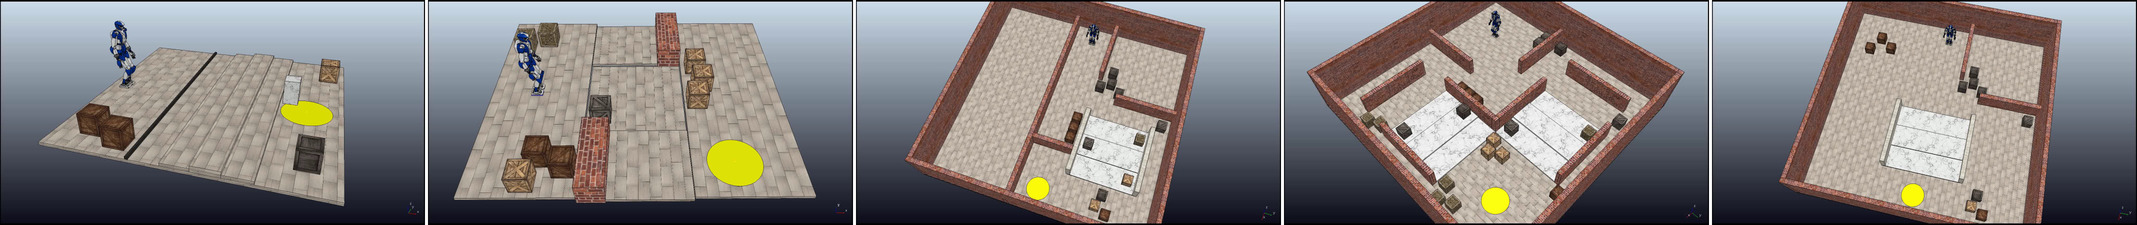
\includegraphics[width=\textwidth]{figures/PlanningScenarios.jpeg}
    \caption{The considered scenarios, from left to right: \textit{Rod}, \textit{Ditch}, \textit{Corridor}, \textit{Maze}, \textit{Spacious}.}
    \label{fig:WoS:Scenarios}
\end{figure}

\begin{figure}
    \centering
    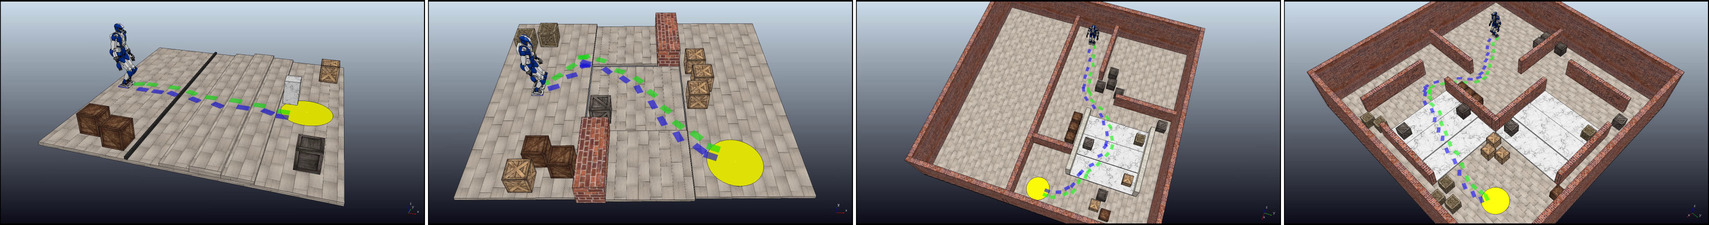
\includegraphics[width=\textwidth]{figures/ExampleResults.jpeg}
    \caption{Examples of footstep plans found in the scenarios \textit{Rod}, \textit{Ditch}, \textit{Corridor} and \textit{Maze}, respectively, when minimizing the number of steps.}
    \label{fig:WoS:ExampleResults}
\end{figure}
\begin{figure}
    \centering
    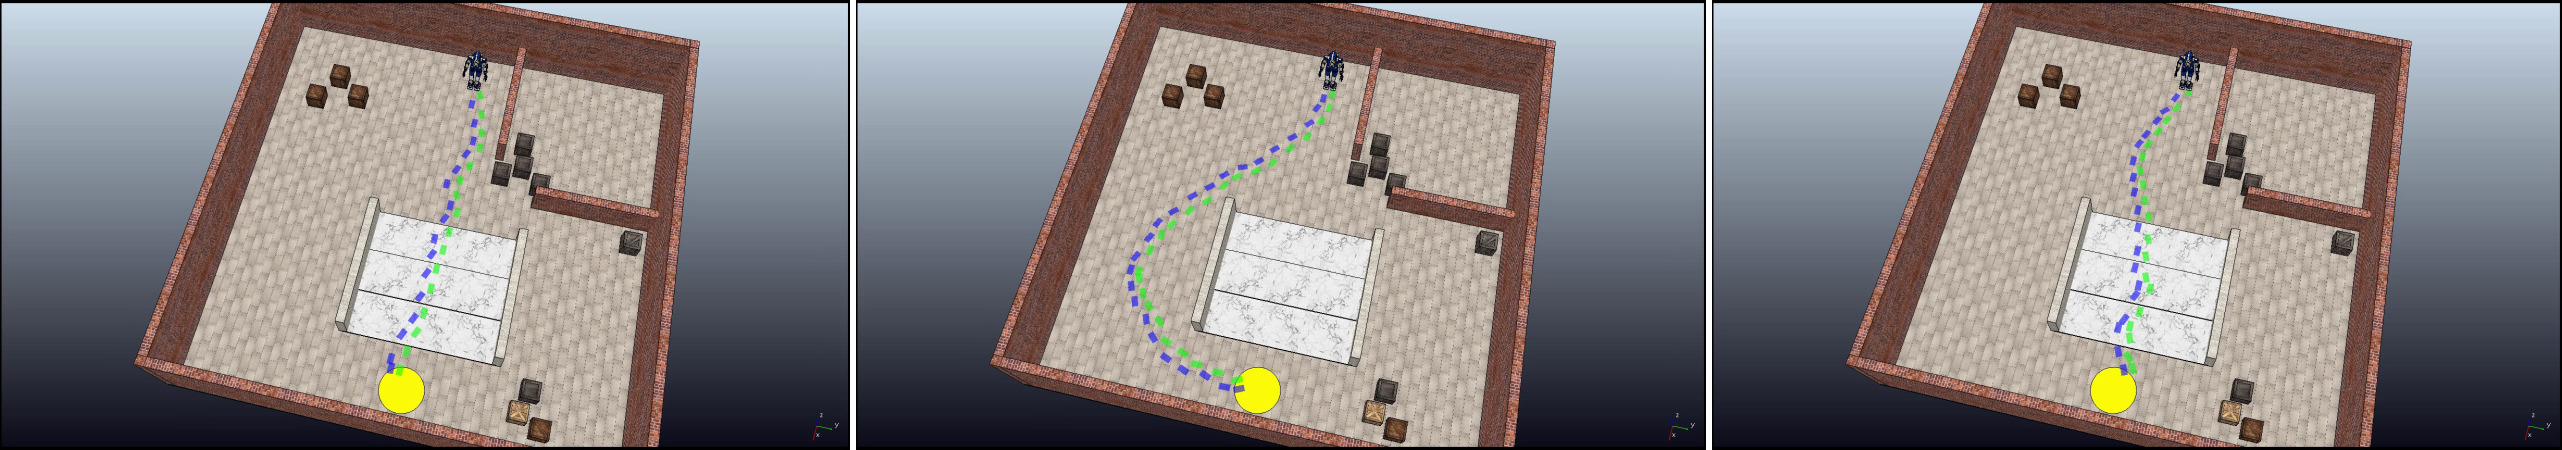
\includegraphics[width=\textwidth]{figures/ExampleResultsCompare.jpeg}
    \caption{Examples of footstep plans found in the scenario \textit{Spacious} when minimizing the number of steps, minimizing the height variation and maximizing the clearance, respectively.}
    \label{fig:WoS:ExampleResultsCompare}
\end{figure}

In all scenarios, the robot has to reach a circular goal region of radius 0.5 m.
The catalogue of primitives $U$ is generated by listing all possible
combinations of the following parameters: longitudinal displacement
$\{-0.08,0.00,0.08,0.16,0.2\}$ [m], lateral displacement $\{0.20,0.30\}$ [m]
for right support and $\{-0.20,-0.30\}$ [m] for left support, angular
displacement $\{0.00,0.40\}$ [rad] for right support and $\{0.00,-0.40\}$ [rad]
for left support (see Fig. \ref{fig:WoS:Primitives}).
In the off-line footstep planner we have set
$k_{\mu} = 1$, $k_{\gamma} = 0$, $h_{\min} = 0.02$~m, $h_{\max} = 0.24$~m,
$\Delta h = 0.02$~m, $\Delta_x^- = 0.08$~m, $\Delta_x^+ = 0.24$~m,
$\Delta_y^-=0.07$~m, $\Delta_y^+=0.07$~m, $\Delta_z^-=0.16$~m,
$\Delta_z^+=0.16$~m, $\Delta_\theta^-=-0.3$~rad, $\Delta_\theta^+=0.3$~rad,
$\ell = 0.25$~m, $z_b=0.3$~m, $h_b=1.2$~m, and $r_b=0.25$~m.
The elevation map $\mathcal{M}_z$ has a resolution of $0.02$~m.
The three quality criteria described in
Sect. \ref{sec:WoS:offlineCase:FP:CostFunctions} are considered in each scenario.

Tables \ref{tab:benchmark:off-line:steps}--\ref{tab:benchmark:off-line:clearance}
show the performance of the planner in each scenario, for different values of
the time budget, when choosing the three optimality criteria described in
Sect. \ref{sec:WoS:offlineCase:FP:CostFunctions}, respectively.
In each table, each row reports the results obtained over 100 runs on a
combination of scenario and time budget. A total of six performance indexes
are tracked and averaged over the total number of successful runs.
In particular, a run is considered unsuccessful if the planner terminates
without placing any footstep in the goal region.
Note that all unsuccessful cases are due to inappropriate time budget.
Examination of the table confirms that increasing the time budget both solves
this problem by ensuring a high success rate, and improves the quality of the
plan in terms of the average cost (Avg Cost). 
This result supports our conjecture about the asymptotic optimality of the
proposed footstep planner.

Figure \ref{fig:WoS:ExampleResults} shows the plans generated by minimizing the
number of steps in the scenarios \textit{Rod}, \textit{Ditch}, \textit{Corridor}
and \textit{Maze}.
In particular, in \textit{Rod} the plan allows to correctly pass over the thin
obstacle and walk the stairway, eventually reaching the goal region; in
\textit{Ditch} the plan reaches the left patch before traversing the low central
patches; in \textit{Corridor} the plan manages to exit the first room, reaching
the stairway and avoiding the obstacles; in \textit{Maze} the plan takes the
left path among the two available, which is the optimal one. 
Figure \ref{fig:WoS:ExampleResultsCompare} compares the plans generated in the
scenario \textit{Spacious} for each considered cost function. 
In particular, when minimizing the number of steps the plan goes straight
towards the goal region; when minimizing the height variation, the plan avoids
the stairway; when maximizing the clearance the plan first moves away from the
wall placed on the left flank of the robot at its starting configuration, and
then moves towards the goal region while keeping the other obstacles at a safe
distance.

\begin{table*}
    \centering
    \scriptsize
    \begin{tabular}{*{8}{c}}
         Scenario & Time Budget [s] & Avg Cost & Min Cost & Max Cost & Iters & Tree Size & Successes \\
        \hline
        \multirow{4}{*}{\textit{Rod}} & 1 & 22.938 & 15.000 & 35.000 & 6393.8 & 2948.7 & 96/100 \\
         & 5 & 19.810 & 15.000 & 28.000 & 21537.8 & 9863.0 & 100/100 \\
         & 10 & 18.050 & 15.000 & 25.000 & 34758.2 & 15705.5 & 100/100 \\
         & 25 & 16.600 & 15.000 & 24.000 & 62862.0 & 27944.5 & 100/100 \\
        
        \hline                                                          
        \multirow{4}{*}{\textit{Ditch}} & 1 & 40.364 & 30.000 & 51.000 & 5966.7 & 2119.5 & 33/100 \\
         & 5 & 36.450 & 27.000 & 47.000 & 18632.4 & 7100.4 & 100/100 \\
         & 10 & 33.420 & 25.000 & 42.000 & 29195.2 & 11503.3 & 100/100 \\
         & 25 & 30.940 & 25.000 & 38.000 & 52090.5 & 20755.6 & 100/100 \\  
        
        \hline                                                            
        \multirow{4}{*}{\textit{Corridor}} & 1 & 57.823 & 51.000 & 68.000 & 6131.4 & 1880.7 & 17/100 \\
         & 5 & 60.213 & 46.000 & 86.000 & 21589.9 & 5068.1 & 89/100 \\
         & 10 & 55.687 & 42.000 & 81.000 & 36426.8 & 8068.1 & 99/100 \\
         & 25 & 49.700 & 42.000 & 60.000 & 70242.7 & 14415.3 & 100/100 \\    

        \hline                                                                      
        \multirow{4}{*}{\textit{Maze}} & 1 & 74.773 & 62.000 & 89.000 & 5813.2 & 2264.9 & 22/100 \\
         & 5 & 70.949 & 54.000 & 94.000 & 21482.0 & 8695.5 & 99/100 \\
         & 10 & 65.520 & 53.000 & 80.000 & 35986.2 & 15327.2 & 100/100 \\
         & 25 & 58.240 & 50.000 & 76.000 & 67507.5 & 28891.7 & 100/100 \\ 

        \hline   
        \multirow{4}{*}{\textit{Spacious}} & 1 & 47.156 & 37.000 & 68.000 & 5749.5 & 2971.2 & 96/100 \\
         & 5 & 41.700 & 35.000 & 55.000 & 20899.7 & 10630.8 & 100/100 \\
         & 10 & 39.290 & 33.000 & 55.000 & 34665.6 & 17412.8 & 100/100 \\
         & 25 & 36.570 & 31.000 & 46.000 & 65308.0 & 31889.3 & 100/100 \\   
    
    \end{tabular}
    \caption{Performance of the off-line footstep planner when minimizing the number of steps.}
    \label{tab:benchmark:off-line:steps}
\end{table*}

\begin{table*}
    \centering
    \scriptsize
    \begin{tabular}{*{8}{c}}
         Scenario & Time Budget [s] & Avg Cost & Min Cost & Max Cost & Iters & Tree Size & Successes \\
        \hline
        \multirow{4}{*}{\textit{Rod}} & 1 & 0.450 & 0.420 & 0.480 & 6634.0 & 3186.5 & 96/100 \\
         & 5 & 0.431 & 0.420 & 0.480 & 20559.8 & 9883.2 & 100/100 \\
         & 10 & 0.425 & 0.420 & 0.480 & 31652.4 & 15140.0 & 100/100 \\
         & 25 & 0.423 & 0.420 & 0.480 & 53598.0 & 25297.7 & 100/100 \\
        
        \hline                                                          
        \multirow{4}{*}{\textit{Ditch}} & 1 & 0.640 & 0.640 & 0.640 & 6218.1 & 2294.4 & 34/100 \\
         & 5 & 0.640 & 0.640 & 0.640 & 17250.0 & 6750.3 & 100/100 \\
         & 10 & 0.640 & 0.640 & 0.640 & 25333.2 & 10171.4 & 100/100 \\
         & 25 & 0.640 & 0.640 & 0.640 & 42419.5 & 17402.7 & 100/100 \\  
        
        \hline                                                            
        \multirow{4}{*}{\textit{Corridor}} & 1 & 0.400 & 0.400 & 0.400 & 6437.1 & 2035.2 & 26/100 \\
         & 5 & 0.400 & 0.400 & 0.400 & 20834.9 & 5288.8 & 92/100 \\
         & 10 & 0.400 & 0.400 & 0.400 & 33405.4 & 8035.9 & 99/100 \\
         & 25 & 0.400 & 0.400 & 0.400 & 61279.5 & 13747.2 & 100/100 \\    

        \hline                                                                      
        \multirow{4}{*}{\textit{Maze}} & 1 & 0.480 & 0.480 & 0.480 & 6170.1 & 2455.4 & 24/100 \\
         & 5 & 0.480 & 0.480 & 0.480 & 20751.2 & 8991.1 & 99/100 \\
         & 10 & 0.480 & 0.480 & 0.480 & 33049.3 & 14808.7 & 100/100 \\
         & 25 & 0.480 & 0.480 & 0.480 & 57441.5 & 26592.6 & 100/100 \\ 
    
        \hline   
        \multirow{4}{*}{\textit{Spacious}} & 1 & 0.346 & 0.000 & 0.400 & 5961.4 & 3254.5 & 97/100 \\
         & 5 & 0.248 & 0.000 & 0.400 & 20470.8 & 11047.0 & 100/100 \\
         & 10 & 0.212 & 0.000 & 0.400 & 32485.0 & 17641.2 & 100/100 \\
         & 25 & 0.168 & 0.000 & 0.400 & 57866.5 & 30630.2 & 100/100 \\       
    
        \end{tabular}
    \caption{Performance of the off-line footstep planner when minimizing the height variation.}
    \label{tab:benchmark:off-line:height}
\end{table*}

\begin{table*}
    \centering
    \scriptsize
    \begin{tabular}{*{8}{c}}
         Scenario & Time Budget [s] & Avg Cost & Min Cost & Max Cost & Iters & Tree Size & Successes \\
        \hline
        \multirow{4}{*}{\textit{Rod}} & 1 & 30.060 & 20.556 & 58.287 & 4925.5 & 2143.6 & 92/100 \\
         & 5 & 25.480 & 18.266 & 42.102 & 16219.7 & 6785.2 & 100/100 \\
         & 10 & 23.142 & 17.586 & 36.173 & 26342.3 & 10602.8 & 100/100 \\
         & 25 & 20.331 & 17.627 & 27.902 & 48444.6 & 18275.1 & 100/100 \\
        
        \hline                                                          
        \multirow{4}{*}{\textit{Ditch}} & 1 & 78.095 & 58.308 & 98.540 & 4200.6 & 1446.2 & 10/100 \\
         & 5 & 72.377 & 54.725 & 99.004 & 13681.3 & 4456.7 & 96/100 \\
         & 10 & 64.840 & 49.282 & 83.708 & 21817.8 & 7302.6 & 100/100 \\
         & 25 & 55.466 & 44.438 & 71.903 & 39632.2 & 13139.3 & 100/100 \\  
        
        \hline                                                            
        \multirow{4}{*}{\textit{Corridor}} & 1 & 94.234 & 72.764 & 112.454 & 4538.3 & 1376.9 & 12/100 \\
         & 5 & 97.323 & 73.304 & 139.995 & 15477.9 & 3418.1 & 82/100 \\
         & 10 & 88.866 & 66.266 & 139.700 & 26354.5 & 5314.1 & 98/100 \\
         & 25 & 78.178 & 64.615 & 102.587 & 52076.3 & 9236.0 & 100/100 \\
        
        \hline                                                                      
        \multirow{4}{*}{\textit{Maze}} & 1 & 107.971 & 95.340 & 127.139 & 4374.8 & 1744.1 & 8/100 \\
         & 5 & 106.620 & 81.630 & 149.408 & 16037.0 & 5919.7 & 88/100 \\
         & 10 & 99.264 & 73.844 & 133.529 & 27154.9 & 10394.0 & 100/100 \\
         & 25 & 84.433 & 65.234 & 119.569 & 52035.2 & 19752.6 & 100/100 \\
        
        \hline   
        \multirow{4}{*}{\textit{Spacious}} & 1 & 52.476 & 32.652 & 85.874 & 4467.9 & 2286.9 & 97/100 \\
         & 5 & 47.138 & 30.160 & 70.100 & 15879.2 & 7689.2 & 100/100 \\
         & 10 & 43.535 & 28.001 & 66.777 & 26325.6 & 12425.1 & 100/100 \\
         & 25 & 38.048 & 27.357 & 57.544 & 49981.9 & 22038.9 & 100/100 \\ 
        
    \end{tabular}
    \caption{Performance of the off-line footstep planner when maximizing the minimum clearance.}
    \label{tab:benchmark:off-line:clearance}
\end{table*}

\subsection{Localization}
\label{sec:WoS:offlineCase:Localization}

The localization module is continuously fed with the RGB-D images gathered by
the head-mounted camera.
Based on such information, it is in charge of updating in real time the estimate
$\hat{\bfs}$ of the pose of the camera frame.
To this end, it uses RTAB-Map \cite{Labbe2019RTABMap}, an open source visual
SLAM library. 
In particular, the visual odometry and graph optimization tool are employed.
The first tracks the features automatically extracted from the RGB-D images,
while the second minimizes the odometry error through a graph-SLAM algorithm
and a loop closure detector.
It is worth mentioning that our architecture is independent from the specific
implementation of the localization module, hence any off-the-shelf visual SLAM
method can be employed in place of RTAB-Map (see assumption A3 in
Sect. \ref{sec:WoS:Formulation}).

Given the pose $\hat{\bfs}$ of the camera frame estimated through visual SLAM
and the measured joint positions, the direct kinematics module produces the
estimates $\hat{\bfp}_{\rm c}$ and $\hat{\bfvarphi}$ of, respectively, the
CoM position and swing foot pose. These are then provided to the gait generation
and kinematic control module to achieve closed-loop control.

\subsection{Simulations}
\label{sec:WoS:offlineCase:Simulations}
We performed simulations on the HRP-4 humanoid robot in the CoppeliaSim
environment. We tested our off-line framework in multiple environments
(Fig. \ref{fig:WoS:Scenarios}). For the gait generation module we have set
$\eta = 3.6$~s$^{-1}$, the single support duration $T_{ss}=0.6$~s, the double
support duration $T_{ds}=0.4$~s, the size of the moving box
$\tilde{d}_x^{\rm z}=\tilde{d}_y^z=d_z^z=0.05$~m, $\beta=1000$, $C=100$ and
$\delta = 0.01$~s. To solve the QP problems we used \texttt{hpipm}, which
requires less than $1$~ms to solve each QP and is thus able to run in real-time
with an ample margin.

Figure \ref{fig:WoS:offlineCase:Ditch:Snapshots} shows the robot traversing the
scenario \textit{Ditch}. The robot starts by moving to its left (first
snapshot), approaching the accessible patch (second snapshot). It then accesses
the platform in the middle correctly avoiding the obstacle (third and fourth
snapshots), eventually reaching the goal region by climbing the final two
patches (fifth and sixth snapshots).
Figure \ref{fig:WoS:offlineCase:Corridor:Snapshots} shows the robot moving
inside the scenario \textit{Corridor}. The robot first exits the room in which
it starts (first and second snapshots), approaching the stairway (third
snapshot). Then, it goes up and down the staircases avoiding the obstacles
(fourth and fifth snapshots), finally reaching the goal region (sixth snapshot).

We invite the reader to watch the video, available at
\url{https://youtu.be/BF43qUcx4gY}, which includes 
clips related to the above simulations as well as additional cases.

\begin{figure}
    \centering
    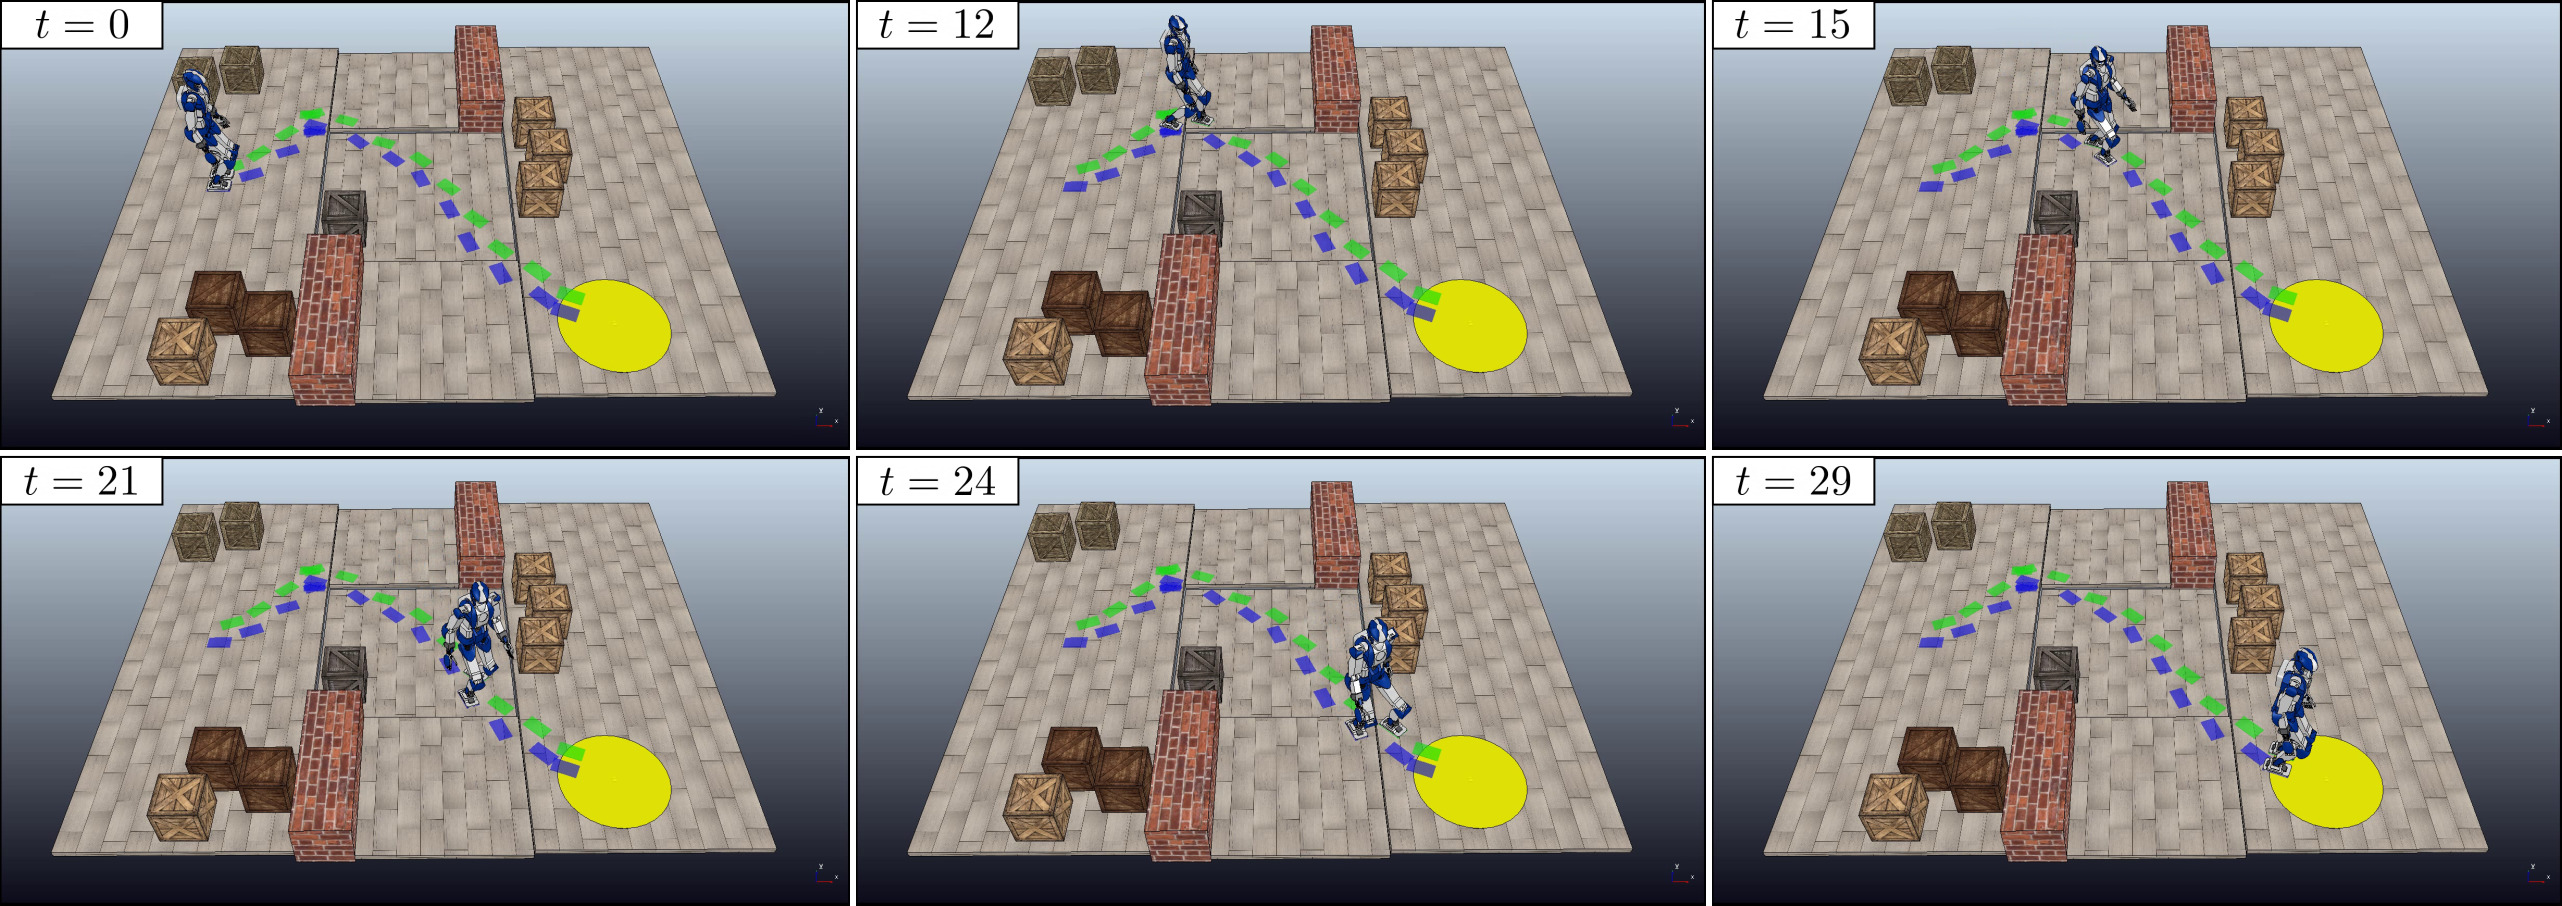
\includegraphics[width=\textwidth]{figures/OfflineDitch.jpeg}
    \caption{The robot reaches the goal going through the ditch, which can only
        be accessed from the left and exited from the right.}
    \label{fig:WoS:offlineCase:Ditch:Snapshots}
\end{figure}
\begin{figure}
    \centering
    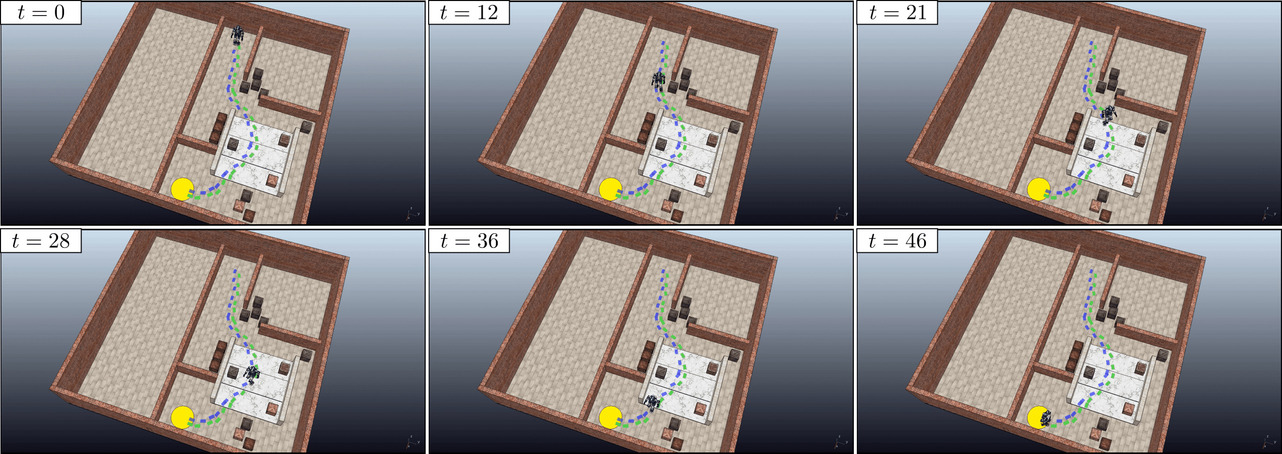
\includegraphics[width=\textwidth]{figures/OfflineCorridor.jpeg}
    \caption{The robot reaches the goal avoiding the
    corridor, climbing and descending the staircase while
    avoiding the obstacles.}
    \label{fig:WoS:offlineCase:Corridor:Snapshots}
\end{figure}


\section{The on-line case} 
\label{sec:WoS:onlineCase}

We now extend the proposed method to the on-line case.
This section starts with a description of the general architecture which,
compared to that proposed for the off-line case, includes two additional
modules, i.e., the mapping and visual task generation module, and employs a
sensor-based version of the footstep planner, which will now work on-line; all
the other modules, in particular gait generation, remain instead identical.  
Then, we describe the mentioned components and present some simulation results.

\subsection{General architecture}
\label{sec:WoS:onlineCase:GeneralArchitecture}
\begin{figure}
\centering
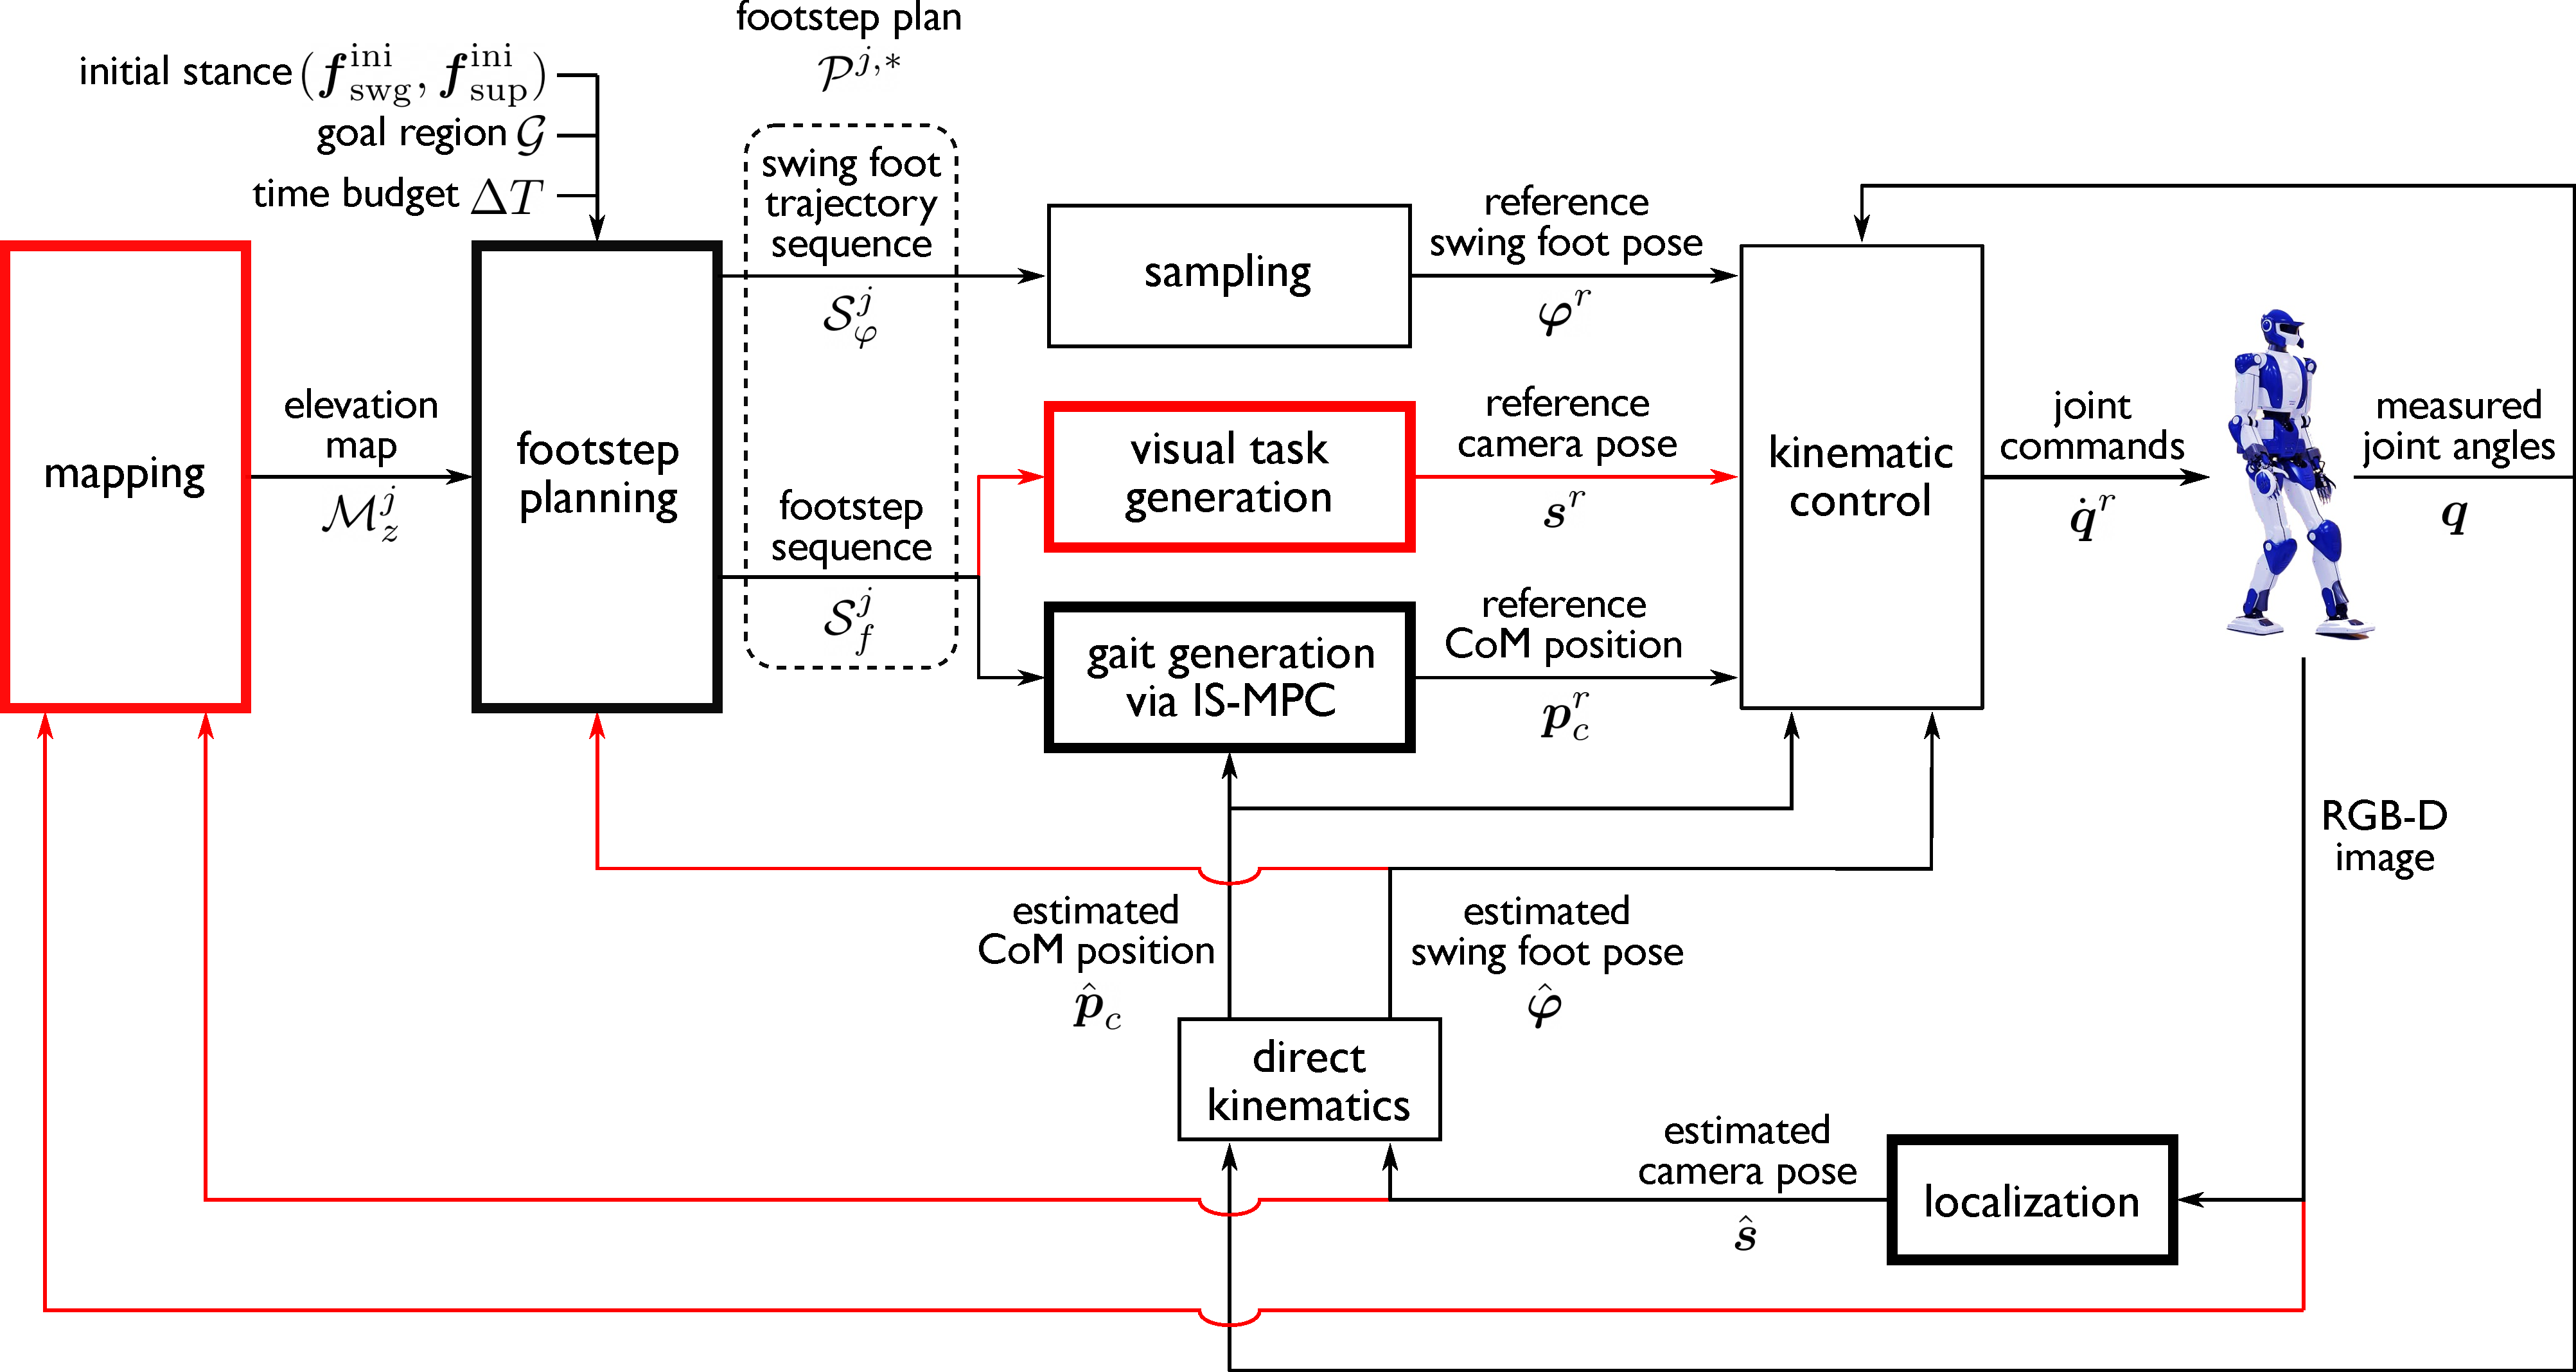
\includegraphics[width=\textwidth]{figures/BlockSchemeOnline.pdf}
\caption{Block scheme of the on-line case. The red blocks and arrows highlight
    the additional modules and signals compared to the off-line case.}
\label{fig:WoS:blockScheme2}
\end{figure}

The proposed architecture for the on-line case is given in
Fig. \ref{fig:WoS:blockScheme2}, where the additional modules and feedback
signals are shown in red.

At the beginning, the map ${\cal M}_z$ is initialized combining some limited
exogenous knowledge about the starting location of the robot and information
available by the head-mounted camera at its initial pose. Such initial map
${\cal M}_z^0$, together with the initial humanoid stance
$(\bff_{\rm swg}^{\rm ini}, \bff_{\rm sup}^{\rm ini})$, the goal region
$\cal G$ and a preassigned time budget $\Delta T$, is provided to the footstep
planner to find a first (possibly partial) footstep plan
${\cal P}^{1,*} = \{ {\cal S}_f^{1}, {\cal S}_\varphi^{1} \}$.

After this initial off-line phase, all the modules run in parallel, generating
the humanoid motions in a sensor-based, closed-loop fashion.
%
The mapping module incrementally builds the elevation map ${\cal M}_z$ using
the RGB-D images acquired by the humanoid while walking and the estimate
$\hat{\bfs}$ of the camera pose produced by the localization module.
To account for changes in ${\cal M}_z$ and take advantage of newly acquired
information, the footstep plan is on-line updated and/or extended by repeatedly
invoking the footstep planner at every step of the humanoid, with the ultimate
objective of reaching $\cal G$. 

More precisely, consider the generic timestamp $t_s^j$, i.e., the beginning of
the $j$-th step.
Let $(\hat{\bff}_{\rm swg}^{j}, \hat{\bff}_{\rm sup}^{j})$ be the current
stance, with $\hat{\bff}_{\rm swg}^{j}$ and $\hat{\bff}_{\rm sup}^{j}$ the
estimates of the swing and support foot poses at $t_s^j$, and
${\cal P}^{j,*} = \{ {\cal S}_f^{j}, {\cal S}_\varphi^{j} \}$ be the current
footstep plan -- computed during the previous ($(j-1)$-th) step -- where the
sequences of footstep placements and associated swing trajectories are defined
as
\begin{gather*}
    {\cal S}_f^j = \{\bff^{j|j}, \dots, \bff^{j+n|j}\}, \\
    {\cal S}_\varphi^j = \{\bfvarphi^{j|j}, \dots, \bfvarphi^{j+n-2|j}\}
\end{gather*}
with their generic elements $\bff^{j+i|j}$ and $\bfvarphi^{j+i|j}$ denoting,
respectively, the $(j+i)$-th footstep and trajectory produced by the $j$-th
planner invocation, $\bff^{j|j} \approx \hat{\bff}_{\rm swg}^{j}$,
$\bff^{j+1|j} \approx \hat{\bff}_{\rm sup}^{j}$ and the last footstep
$\bff^{j+n|j}$ henceforth referred to as \textit{subgoal}.
Also, let $(\bff_{\rm swg}^{j+1}, \bff_{\rm sup}^{j+1})$ be the stance that the
humanoid is supposed to achieve at $t_s^{j+1} = t_s^j + T_s^j$, with
$\bff_{\rm swg}^{j+1} = \hat{\bff}_{\rm sup}^{j}$ and
$\bff_{\rm sup}^{j+1} = \bff^{j+2|j}$, after performing the swing trajectory
$\bfvarphi^{j|j}$ having duration $T_s^j$.
%
Then, during the time interval $[t_s^j, t_s^{j+1})$, motion execution and
footstep planning take place simultaneously as follows.
\begin{itemize}
    \item At any time instant $t \in [t_s^j, t_s^{j+1})$, the current reference
        position $\bfp_{\rm c}^r$ of the CoM is produced by the gait generator,
        based on the sequence ${\cal S}_f^j$, similarly to the off-line case;
        the current reference pose $\bfvarphi^r$ of the swing foot is obtained
        by sampling the trajectory $\bfvarphi^{j|j}$; moreover, the visual task
        generator produces the reference pose $\bfs^r$ of the camera frame,
        given its current estimate $\hat{\bfs}$ and the sequence ${\cal S}_f^j$,
        that allows to direct the gaze towards the subgoal extracted from
        ${\cal S}_f^j$, and then to enlarge ${\cal M}_z$ in the area of the
        current destination. 
        References $\bfp_{\rm c}^r$, $\bfvarphi^r$, $\bfs^r$, together with
        their estimates $\hat{\bfp}_{\rm c}$, $\hat{\bfvarphi}$, $\hat{\bfs}$,
        are passed to the kinematic controller to compute the joint commands
        $\dot{\bfq}^r$ for the robot.
    \item At $t_s^j$, the footstep planner is invoked providing in input the
        stance $(\bff_{\rm swg}^{j+1}, \bff_{\rm sup}^{j+1})$, the goal region
        $\cal G$, a time budget equal to $T_s^j$, and the elevation map
        ${\cal M}_z^j$ currently available by the mapping module.
        At $t_s^{j+1}$, the planner returns a new footstep plan
        ${\cal P}^{j+1,*} = \{ {\cal S}_f^{j+1}, {\cal S}_\varphi^{j+1}\}$, where
        the sequences ${\cal S}_f^{j+1}$ and ${\cal S}_\varphi^{j+1}$ are
        defined similarly to ${\cal S}_f^{j}$ and
        ${\cal S}_\varphi^{j}$, $\bff^{j+1|j+1} = \bff_{\rm swg}^{j+1}$ and
        $\bff^{j+2|j+1} = \bff_{\rm sup}^{j+1}$. 
        The first element $\bfvarphi^{j+1|j+1}$ of ${\cal S}_\varphi^{j+1}$ will
        define the next ($(j+1)$-th) step of the humanoid. 
\end{itemize}

Note that, while the footstep planner will make use of a fixed map
$\mathcal{M}_z^j$ during the time interval $[t_s^j, t_s^{j+1})$, the map
$\mathcal{M}_z$ will continuously be updated by the mapping module during the
same time interval, which will generally provide a different map
$\mathcal{M}_z^{j+1}$ for the next invocation of the planner.

Clearly, in the on-line case, only the quality of the partial footstep plans can
be accounted for, ultimately leading to an overall plan that is globally suboptimal. 

\subsection{Mapping}
\label{sec:WoS:onlineCase:MappingModule}
At the generic time instant, the mapping module receives in input the last RGB-D
image acquired by the head-mounted camera and the current estimate $\hat{\bfs}$
of the camera pose produced by the localization module. 
It is responsible for integrating such newly acquired information into the
elevation map $\mathcal{M}_z$.

First, the depth data extracted from the RGB-D image are used to construct a
point cloud.
Then, the latter is given in input, together with the estimate $\hat{\bfs}$ and
a sensor noise model, to Elevation Mapping
\cite{Fankhauser2018ProbabilisticTerrainMapping}, an open source framework
designed for rough terrain mapping; this accordingly updates a local
(limited around the robot)
representation of the environment in the form of a 2.5D grid map (see
Assumption A1). Finally, such local map is integrated into $\mathcal{M}_z$ in
order to maintain a global representation of the explored area of the environment.

The mapping module, at the time $t_s^j$ of the generic $j$-th invocation of
the footstep planner, provides it with a copy $\mathcal{M}_z^j$ of the available
map $\mathcal{M}_z$.
Meanwhile, during the planner operation, the map $\mathcal{M}_z$ is continuously
updated through the process described above.

\subsection{Sensor-based footstep planning}
\label{sec:WoS:onlineCase:FootstepPlanner}
This module consists in a sensor-based version of the footstep planner proposed
in Sect. \ref{sec:WoS:offlineCase:FootstepPlanner} which works using the
knowledge about the environment incrementally acquired by the robot during motion. 
We now describe the footstep planning algorithm for the on-line case (Algorithm
\ref{alg:AnytimeFootstepPlanner}).

\begin{algorithm}%[!t]
	\small
	\removelatexerror
    %\caption{SensorBasedFootstepPlanner$(({\bff}_{\rm swg}^{j+1}, {\bff}_{\rm sup}^{j+1}), {\cal G}, {\Delta T}^j, {\cal M}_z^j)$}
	
	\caption{SensorBasedFootstepPlanner}
	\label{alg:AnytimeFootstepPlanner}

	\KwIn{$({\bff}_{\rm swg}^{j+1}, {\bff}_{\rm sup}^{j+1}), {\cal G}, {\Delta T}^j, {\cal M}_z^j$}
	\vspace{2pt}
	\KwOut{${\cal P}^{j+1,*}$}
    \BlankLine

    $({\cal T}^{j+1}, v^{\rm root})$ $\leftarrow$ InitializeTree$({\cal T}^j, ({\bff}_{\rm swg}^{j+1}, {\bff}_{\rm sup}^{j+1}))$\; 
	
    ${\cal V}_{\rm child}$ $\leftarrow$ ChildVertexes$({\cal T}^{j+1}, v^{\rm root})$\;
	\ForEach{$v'$ $\in$ ${\cal V}_{\rm child}$}{
        UpdateTree$({\cal T}^{j+1}, v', {\cal M}_z^j)$\;
    } 	

	ExpandTree$({\cal T}^{j+1}, {\Delta T}^j - {\Delta T}_{\rm e}, {\cal M}_z^j)$\;

	${\cal P}^{j+1,*}$ $\leftarrow$ RetrieveBestPlan$({\cal T}^{j+1}, {\cal G})$\;
    \Return{${\cal P}^{j+1,*}$}\;
\end{algorithm}

The input data for the $j$-th invocation of the footstep planner are the next
robot stance $(\bff_{\rm swg}^{j+1}, \bff_{\rm sup}^{j+1})$, the goal region
$\cal G$, the time budget ${\Delta T}^j$ and the elevation map ${\cal M}_z^j$. 
Given an optimality criterion, the footstep planner returns the best footstep
plan ${\cal P}^{j+1,*}$, found within ${\Delta T}^j$, either leading to $\cal G$
or terminating in proximity of the frontier of ${\cal M}_z^j$.
The latter case is typical whenever $\cal G$ is not included in ${\cal M}_z^j$,
e.g., due to occlusions or simply being placed far from the robot.

The planning algorithm builds a tree $\mathcal{T}^{j+1}$ reusing portions of
the tree $\mathcal{T}^{j}$ built up to the previous invocation. 
In this tree, vertexes and edges are defined as described in
Sect. \ref{sec:WoS:offlineCase:FootstepPlanner}, with the only difference that
a vertex $v = (\bff_{\rm swg}, \bff_{\rm sup})$ can contain a support footstep
$\bff_{\rm sup}$ whose $z$-coordinate is unspecified, indicating that
${\cal M}_z^j$ does not provide enough information (in a sense formally defined
in the following) about the ground under the foot at $\bff_{\rm sup}$. 
Vertexes with this characteristic represent stances located on the frontier of
${\cal M}_z^j$ and thus indicate possible direction for further exploration of
the environment. 
%
The generic invocation consists of: initializing, updating and expanding the
tree. These individual steps are described in the following.

{\bf Initializing}: The vertex $v^{\rm root} = (\bff_{\rm swg}^{\rm root}, \bff_{\rm sup}^{\rm root})$ of $\mathcal{T}^{j}$ that is closest to $(\bff_{\rm swg}^{j+1}, \bff_{\rm sup}^{j+1})$ is identified. To this end, we define a stance-to-stance metric as
\begin{equation}
    \label{eq:WoS:metricIdentifyRoot}
    \zeta(v, v') = \gamma(\bff_{\rm swg}, \bff'_{\rm swg}) + \gamma(\bff_{\rm sup}, \bff'_{\rm sup}) 
\end{equation}
where $\gamma(\cdot)$ is the footstep-to-footstep metric defined in
(\ref{eq:WoS:footstepToFootstepMetric}).
The subtree of $\mathcal{T}^{j}$ rooted at $v^{\rm root}$ is extracted
(including $v^{\rm root}$ itself) and represents the initial version of
$\mathcal{T}^{j+1}$.
To match the stance that the humanoid is supposed to reach at the end of the
simultaneously executed step, $v^{\rm root}$ is modified by relocating
$\bff_{\rm swg}^{\rm root}$ to $\bff_{\rm swg}^{j+1}$ and
$\bff_{\rm sup}^{\rm root}$ to $\bff_{\rm sup}^{j+1}$.
This step corresponds to Procedure \ref{proc:InitializeTree}.
\hfill $\blacktriangleleft$
\begin{procedure}%[!t]
	\small
	\removelatexerror
	%\caption{InitializeTree(${\cal T}^j$, ($\bff_{\rm swg}^{j+1}$, $\bff_{\rm sup}^{j+1}$))}
	\caption{InitializeTree()}
	\label{proc:InitializeTree}

	\KwIn{${\cal T}^j, (\bff_{\rm swg}^{j+1}, \bff_{\rm sup}^{j+1}))$}
	\vspace{2pt}
	\KwOut{${\cal T}^{j+1}, v^{\rm root}$}
    \BlankLine
	
	$v^{\rm root}$ $\leftarrow$ NearestVertex$({\cal T}^j, (\bff_{\rm swg}^{j+1}, \bff_{\rm sup}^{j+1}))$\;
	
	${\cal T}^{j+1}$ $\leftarrow$ ExtractSubtree$({\cal T}^j, v^{\rm root})$\;
	
	UpdateVertex$({\cal T}^{j+1}, v^{\rm root}, (\bff_{\rm swg}^{j+1}, \bff_{\rm sup}^{j+1}))$\;
	
    \Return{$({\cal T}^{j+1}, v^{\rm root})$}\;
	
\end{procedure}

{\bf Updating}: At this point, requirements R1--R3 are satisfied by
construction in $\mathcal{T}^{j+1}$ according to the previous map
$\mathcal{M}_z^{j-1}$.
Then, R1--R3 must now be checked in $\mathcal{T}^{j+1}$ using the most recent
map $\mathcal{M}_z^{j}$, consequently updating vertexes and edges in order to
satisfy them.
To this end, we perform a pre-order traversal of $\mathcal{T}^{j+1}$ as
described in the following.

When a vertex $v = (\bff_{\rm swg}, \bff_{\rm sup})$ is visited, it is
modified\footnote{This modification is not made on $v^{\rm root}$ as it
corresponds to the stance that the robot must reach at the end of the
simultaneously executed step.} by relocating its swing footstep to the support
footstep $\bff_{\rm sup}^{\rm parent}$ of its parent
$v^{\rm parent} = (\bff_{\rm swg}^{\rm parent}, \bff_{\rm sup}^{\rm parent})$,
and setting the $z$ coordinate $z_{f, \rm sup}$ of $\bff_{\rm sup}$ according
to $\mathcal{M}_z^{j}$.
In particular, consider the cells of ${\cal M}_z^j$ belonging to, or
overlapping with, the footprint at $\bff_{\rm sup}$; let $n_{\rm k}$ and
$n_{\rm u}$ be the number of these cells whose height is known and unknown,
respectively. If the rate of cells with known height is larger than a predefined
threshold $\bar{n}$, i.e.,
\begin{equation*}
    \frac{n_{\rm k}}{n_{\rm k} + n_{\rm u}} > \bar{n},    
\end{equation*}
$z_{f, \rm sup}$ is set to the average value of the $n_{\rm k}$ known heights. 
Otherwise, $z_{f, \rm sup}$ is left unspecified.

Once $v$ has been updated, requirements R1--R3 are checked similarly to what
was done in the off-line case, with the only two differences described in the
following.
\begin{itemize}
    \item If $z_{f, \rm sup}$ is unspecified, requirements R1--R3 are checked
        conjecturing that it is equal to the $z$-component $z_{f, \rm swg}$ of
        $\bff_{\rm swg}$.
    %
    \item Requirement R1 is considered satisfied if for each of the $n_{\rm k}$
        known heights, the net variation from $z_{f, \rm sup}$ does not exceed
        a predefined threshold $\bar{z}$, i.e.,
        \begin{equation*}
            |z_{\rm k} - z_{f, \rm sup}| \leq \bar{z}.
        \end{equation*}
        with $z_{\rm k}$ the generic known height among the $n_{\rm k}$ available.
\end{itemize}

If any requirement among R1--R3 is violated, vertex $v$ is removed from
$\mathcal{T}^{j+1}$, along with its descendants.
Otherwise, the edge connecting $v$ to $v^{\rm parent}$ is replaced by the
trajectory $\bfvarphi^{\rm parent}$ generated while checking R3; the set
${\cal V}_{\rm child}$ of child vertexes of $v$ is retrieved, and the procedure
is recursively invoked on them. 
To guarantee on-line performance and save time to be used for expanding
$\mathcal{T}^{j+1}$, recursion is stopped on vertexes having a maximum depth
$\bar{\kappa}$.
This step corresponds to Procedure \ref{proc:UpdateTree}.
\begin{procedure}%[!t]
	\small
	\removelatexerror
	
    %\caption{UpdateTree(${\cal T}^{j+1}$, $v$, ${\cal M}_z^j$)}
    \caption{UpdateTree()}
	\label{proc:UpdateTree}

	\KwIn{${\cal T}^{j+1}, v, {\cal M}_z^j$}
	\vspace{2pt}
	\KwOut{none}
    \BlankLine
	
	$v^{\rm parent}$ $\leftarrow$ ParentVertex$({\cal T}^{j+1}, v)$\;
    
    $z_{f, \rm sup}$ $\leftarrow$ DetermineFootstepHeight$(\bff_{\rm sup}, {\cal M}_z^j)$\;
    
    UpdateVertex$({\cal T}^{j+1}, v, (\bff_{\rm sup}^{\rm parent}, (x_{f, \rm sup}, y_{f, \rm sup}, z_{f, \rm sup})))$\;
    
    \eIf{\rm R1$(\bff_{\rm sup})$ \rm \textbf{and} \rm R2$(\bff_{\rm sup}$, $\bff^{\rm parent}_{\rm sup})$}{
 	 	$\bfvarphi^{\rm parent}$ $\leftarrow$ SwingTrajectoryEngine$(\bff_{\rm swg}^{\rm parent}, \bff_{\rm sup})$\;
	 	
	 	\eIf{\rm R3$(\bfvarphi^{\rm parent}, (\bff_{\rm swg}, \bff_{\rm sup}))$}{
            UpdateEdge$({\cal T}^{j+1}, v^{\rm parent}, v, \bfvarphi^{\rm parent})$\;
            
            \If{\rm Depth$({\cal T}^{j+1}, v))$ = $\bar\kappa$}{
                \Return\;    	
            } 	
            
            ${\cal V}_{\rm child}$ $\leftarrow$ ChildVertexes$({\cal T}^{j+1}, v)$\;
            \ForEach{$v'$ $\in$ ${\cal V}_{\rm child}$}{
                UpdateTree$({\cal T}^{j+1}, v', {\cal M}_z^j)$\;
            }
             	   
	 	} 
	 	{
	 	    RemoveSubtree$({\cal T}^{j+1}, v)$\; 	
	 	}
 	}
	{
 	    RemoveSubtree$({\cal T}^{j+1}, v)$\; 	
 	}
	 
    \Return\;   
	
\end{procedure}
\hfill $\blacktriangleleft$

{\bf Expanding}: Once $\mathcal{T}^{j+1}$ has been updated, it can be further
expanded in the map $\mathcal{M}_z^j$.
Let ${\Delta T}_{\rm e}$ be the time elapsed since the beginning of the current
invocation of the footstep planner, i.e., the time spent in initializing and
updating $\mathcal{T}^{j+1}$.
The expansion of $\mathcal{T}^{j+1}$ works iteratively as described in
Sect. \ref{sec:WoS:offlineCase:FP:PlannerOverview} using the remaining portion
of the time budget ${\Delta T}^j - {\Delta T}_{\rm e}$ and the map
$\mathcal{M}_z^j$, with the following modifications.
\begin{itemize}
    \item The choice of the $z$-coordinate for a candidate footstep
        $\bff_{\rm sup}^{\rm cand}$ and the check of requirements R1--R3 are
        done exactly as when updating a generic vertex. 
    \item A vertex whose support footstep has unspecified $z$-coordinate
        cannot be set as parent of another vertex.
        Then, such vertexes are excluded both when selecting the vertex
        $v^{\rm near}$ for an expansion attempt and when choosing a parent for
        a candidate vertex $v^{\rm cand}$. \hfill $\blacktriangleleft$
\end{itemize} 

Similarly to the off-line case, when the assigned time budget ${\Delta T}^j$
runs out, tree expansion is stopped and the set ${\cal V}_{\rm goal}$ of
vertexes $v$ such that $\bfp_{f,{\rm sup}} \in {\cal G}$ is retrieved.
%
If ${\cal V}_{\rm goal}$ is not empty, the vertex $v^*$ with minimum cost is
selected as in (\ref{eq:WoS:BestVertex}).
%
Otherwise, if ${\cal V}_{\rm goal}$ is empty, the planner retrieves the set
${\cal V}_{\rm fron}$ containing all vertexes of $\mathcal{T}^{j+1}$ having at
least one child vertex whose support footstep has unspecified $z$-coordinate.
In practice, vertexes in ${\cal V}_{\rm fron}$ contain stances located in
proximity of the frontier of the current map $\mathcal{M}_z^j$.
Then, the vertex $v^*$ is selected as
\begin{equation}
    \label{eq:WoS:BestVertexSubgoal}
    v^* = \underset{v \in {\cal V}_{\rm fron}}{\arg\!\min} \ c(v)+g(v)
\end{equation}
where $g(v)$ represents the \textit{cost-to-go} of vertex $v$, i.e., a
lower-bound on the minimum cost to reach $\mathcal{G}$ from $v$.
A possible choice for $g(v)$ when minimizing the number of steps along the
plan will be described in Sect. \ref{sec:WoS:onlineCase:Simulations}.

Finally, the footstep plan ${\cal P}^{j+1,*}$ is retrieved from the branch of
$\mathcal{T}^{j+1}$ joining the root to $v^*$. 
Clearly, if ${\cal V}_{\rm goal}$ is not empty, ${\cal P}^{j+1,*}$ will be a
complete footstep plan leading to $\mathcal{G}$; otherwise, ${\cal P}^{j+1,*}$
will be a partial footstep plan leading in the direction of an unknown area of
the environment whose exploration is considered useful -- according to the
adopted cost-to-go -- to proceed towards $\mathcal{G}$. 

\subsection{Visual task generation}
\label{sec:WoS:onlineCase:VisualTaskGeneration}
At any time instant during the execution of the generic $j$-th step, given the
current estimate $\hat{\bfs}$ of the camera pose and the subgoal $\bff^{j+n|j}$,
which is readily extracted from the current sequence $\mathcal{S}_f^j$ of
footstep placements, the visual task generator is in charge of producing a
suitable reference $\bfs^r$ of the camera pose which aims at directing the gaze
towards the current destination of the robot. 
The rationale beyond this choice is that, since the current footstep plan
terminates in an area on the frontier of the map $\mathcal{M}_z$ that is
considered promising for goal-oriented exploration of the environment, looking
in the direction of $\bff^{j+n|j}$ allows to enlarge the map in that particular
area. In principle, whenever possible, this will privilege further extension of
the footstep plan in that promising direction.

To compute $\bfs^r$, one possibility consists in adopting an image-based visual
servoing scheme \cite{Chaumette2016VisualServoing}. 
In particular, one may define a virtual feature in the image plane of the camera
at $\hat{\bfs}$ associated to the representative point $\bfp_f^{j+n|j}$ of the
subgoal footstep $\bff^{j+n|j}$.
Then, the reference pose $\bfs^r$ of the camera frame can be computed so as to
keep such feature at the center of the image plane.

The produced reference pose $\bfs^r$ is passed to the kinematic controller
which, in practice, only controls the camera yaw and pitch angles.

\subsection{Simulations}
\label{sec:WoS:onlineCase:Simulations}

\begin{figure}
    \centering
    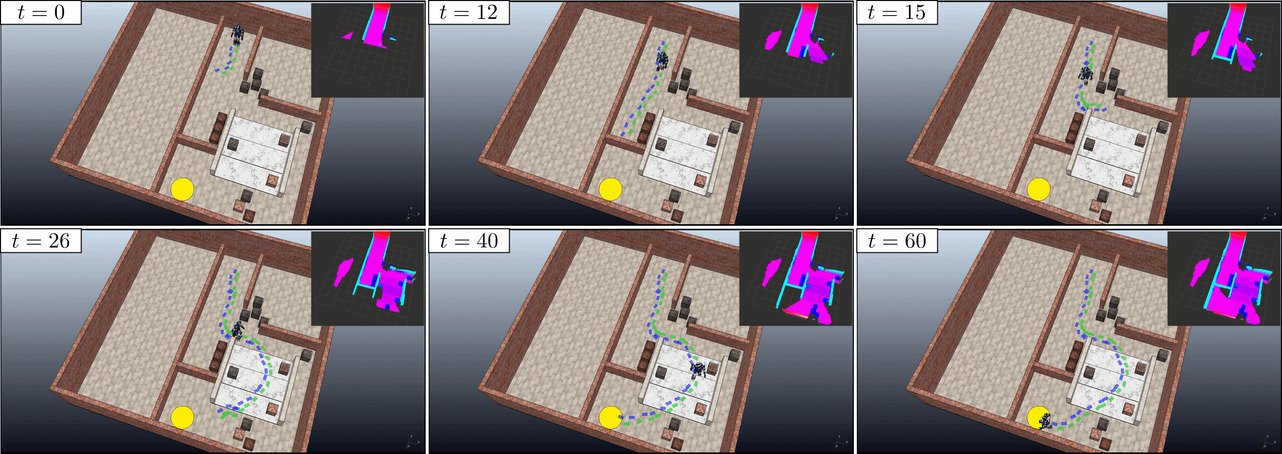
\includegraphics[width=\textwidth]{figures/OnlineCorridor.jpeg}
    \caption{The on-line footstep planner in the scenario \textit{Corridor} minimizing the number of steps. Here the planner finds a footstep sequence of 54 steps.}
    \label{fig:WoS:onlineCase:Corridor:Simulation}
\end{figure}
\begin{figure}
    \centering
    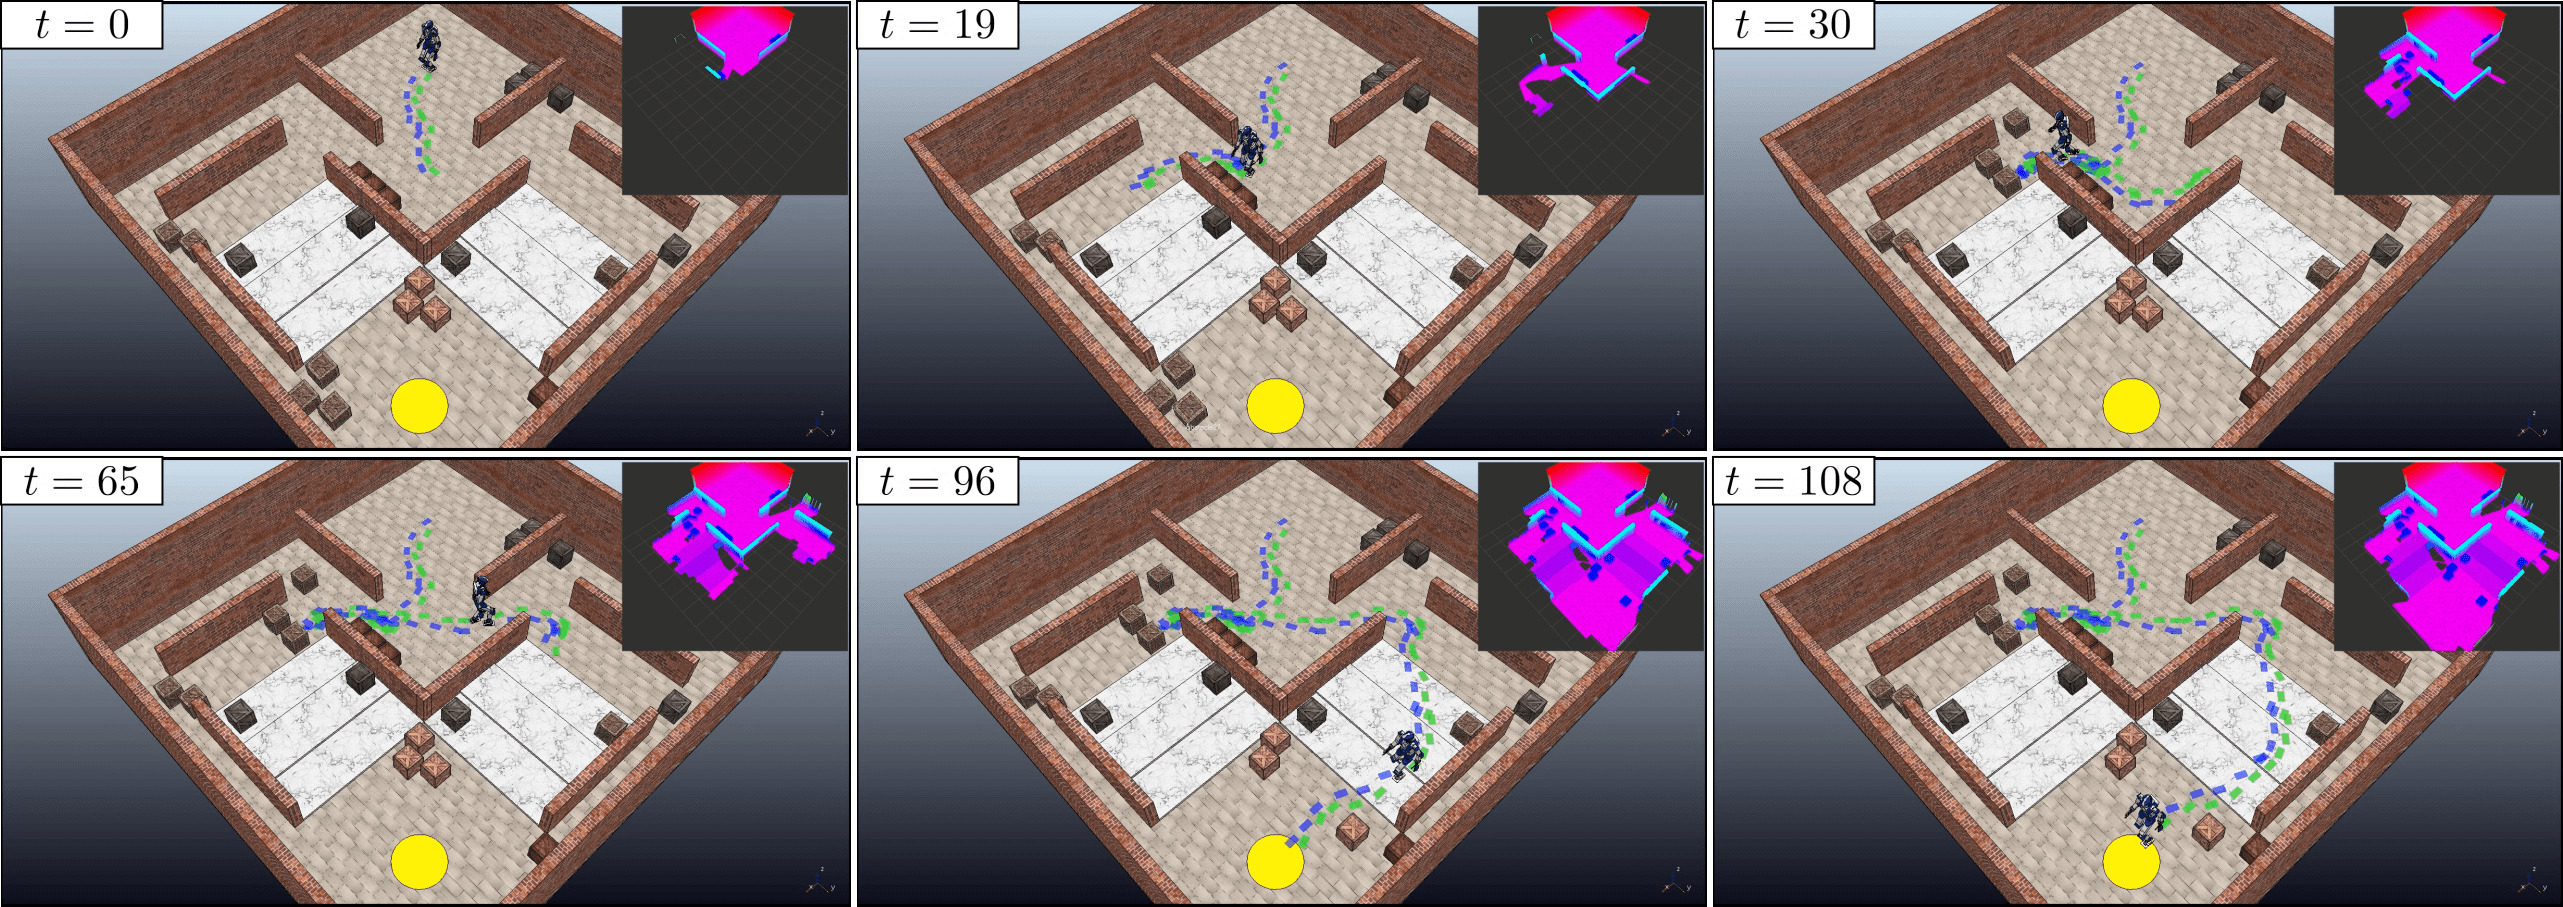
\includegraphics[width=\textwidth]{figures/OnlineMazeDynamic.jpeg}
    \caption{The on-line footstep planner in the environment \textit{Maze} minimizing the number of steps. The environment is dynamic, namely the elevation map can be changed by moving obstacles around. Here the planner finds a footstep sequence of 106 steps.}
    \label{fig:WoS:onlineCase:MazeDynamic:Simulation}
\end{figure}
\begin{figure}
    \centering
    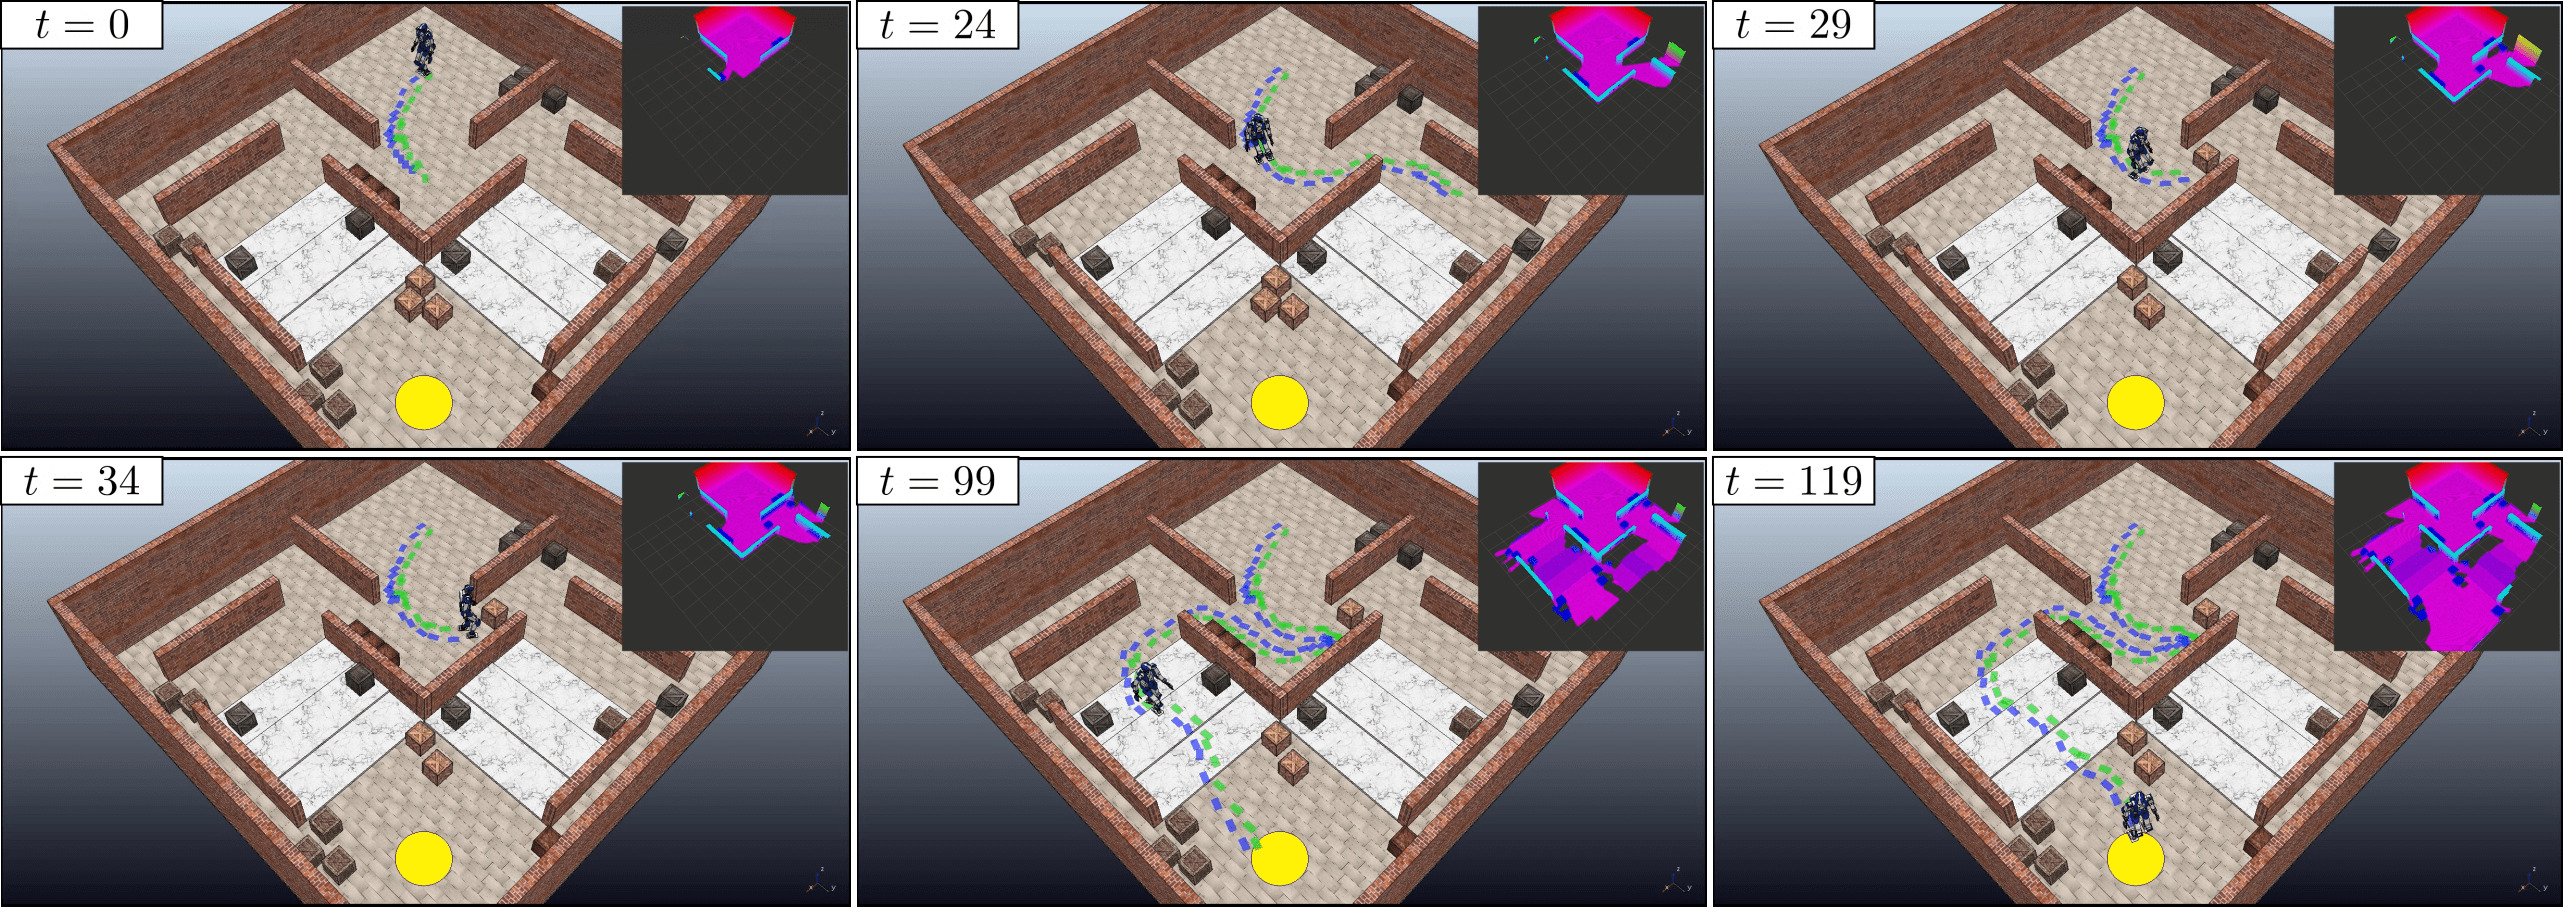
\includegraphics[width=\textwidth]{figures/OnlineMazeStopandgo.jpeg}
    \caption{The on-line footstep planner in the dynamic environment \textit{Maze} minimizing the number of steps. Here the planner finds a footstep sequence of 103 steps.}
    \label{fig:WoS:onlineCase:MazeStopAndGo:Simulation}
\end{figure}

In this section we present simulations obtained with the discussed architecture
for the on-line case. Parameters are set to the same values of
Sect. \ref{sec:WoS:offlineCase:Simulations}, with the only exception of setting
$k_\gamma = 1$ in \eqref{eq:WoS:footstepToFootstepMetric} when used in
\eqref{eq:WoS:metricIdentifyRoot}, $\bar{n}=0.9$, $\bar{z}=0.02$ and
${\bar{\kappa}}=5$. For each $j$-th invocation of the footstep planner the time
budget $\Delta T^j$ is set to $T_{ss}+T_{ds}$. In all performed simulations,
the quality criteria considered by the footstep planner is the number of steps,
while the \textit{cost-to-go} of each vertex $v$ is an underestimation of the
number of steps needed to reach the goal region $\mathcal{G}$ from the double
support configuration specified by $v$. This value is computed as the distance
between the position of the support foot specified by $v$ and $\mathcal{G}$,
divided by the longest step among the catalogue of primitives $U$. 

Figure \ref{fig:WoS:onlineCase:Corridor:Simulation} shows the robot walking in
the scenario \textit{Corridor} together with the reconstructed elevation map.
Here, the planner continuously receives an updated version of the map, which is
built while the robot moves. Initially (first snapshot) the robot starts
exploring its surrounding environment, moving towards the end of the corridor
(second snapshot). As soon as the footstep planner realizes that the room is
closed, it replans a sequence of footsteps which brings the robot outside the
corridor (third snapshot). The robot keeps exploring the environment, going up
and down the stairs and avoiding the obstacles placed along the path (fourth
and fifth snapshot). Finally, the robot reaches the desired goal region (sixth
snapshot).

Figure \ref{fig:WoS:onlineCase:MazeDynamic:Simulation} shows the robot
accomplishing the locomotion task in the scenario \textit{Maze}. In this
case the scenario was rendered dynamic by manually moving the obstacles at
runtime. Here, the planner is facing the additional challenge of operating under
continuous changes in the elevation map, which reflects the new locations of the
obstacles. The robot starts by moving outside the initial room (first snapshot),
choosing the path on its right (second snapshot). The footstep plan is
invalidated by placing obstacles in front of the robot, forcing the robot to
choose the other direction (third snapshot). The footstep planner correctly
drives the robot towards the other area of the maze (fourth snapshot), making it
go up and down the staircase (fifth snapshot), avoiding another obstacle which
is placed in front of the robot right before reaching the goal region (sixth
snapshot).

Figure \ref{fig:WoS:onlineCase:MazeStopAndGo:Simulation} shows a situation,
again in a dynamic version of the scenario \textit{Maze}, in which the planner
reaches a point in which is not able to find a new subgoal. This occurs when,
once the time budget expires, both $\mathcal{V}_{\rm goal}$ and
$\mathcal{V}_{\rm fron}$ are empty.
For example, this may happen when the humanoid must exit a long corridor or when
dynamic obstacles invalidate large portion of the created tree.
In this specific situation, a simple solution consists in keeping the portion of
the current footstep plan that is still valid after the updating step of the
planner. If this happens multiple times in a row, the robot reaches the subgoal
and stops. At this point, the footstep planner is invoked with an unlimited time
budget and terminates as soon as a new subgoal is found. As before, the robot
starts by moving outside the initial room, moving towards its left (first and
second snapshots). The footstep plan is invalidated by moving an obstacle in
front of the robot (third snapshots), which stops its motion upon reaching the
current subgoal (fourth snapshot). As soon as the footstep planner finds a new
subgoal, the robot starts moving again (fifth snapshot), eventually reaching the
desired goal region (sixth snapshot).

Clips of the described simulations are
available at the following link: \url{https://youtu.be/BF43qUcx4gY}.

\section{Discussion}
\label{sec:WoS:discussion}
The proposed approach integrates several components and is designed to work both
off-line and on-line. 
Since, to the best of our knowledge, no existing method can address the same
wide range of situations, we focus in the following on the two main components
(footstep planning and gait generation) separately.

As a representative of the state of the art in footstep planning, we selected
the algorithm in~\cite{Griffin2019ICRA}, which uses a weighted $A^\ast$
algorithm to search for optimal footstep sequences on uneven
ground\footnote{The algorithm in~\cite{Griffin2019ICRA} actually contemplates
the possibility of tilted surfaces, but obviously works in a world of stairs as
a particular case.}. At each iteration, the vertex providing the lowest estimate
for the path cost is expanded. This estimate is computed by adding to the cost
of the vertex a heuristic cost-to-go, given by the distance to the goal divided
by the maximum step length and multiplied by a weight $w\ge 1$, which can be
used to increase the bias towards the goal region. The main difference with
respect to our approach lies in the expansion mechanism, which is deterministic
in~\cite{Griffin2019ICRA} and probabilistic in our method. 

Both our scheme and the weighted $A^\ast$ approach use a catalogue of
primitives. In order to perform a fair comparison, we use for the weighted
$A^\ast$ approach the same catalogue described in
Sect.~\ref{sec:WoS:offlineCase:FP:PlanningResults}. As for the optimality
criterion, we aim to minimize the number of footsteps, corresponding to an edge
cost given by (\ref{eq:WoS:costSteps}). In order to allow for the possibility
that our implementation might not be the most efficient, we assigned to the
weighted $A^\ast$ planner a time budget of $100$~s, which is four times the
largest budget used when testing our planner. 

The results obtained showed that standard $A^\ast$ search, corresponding to
$w=1$, is unable to find solutions within the allotted time budget in any of
the considered scenarios. 
By increasing $w$, weighted $A^\ast$ performs rather well in scenarios where
the solution does not involve considerable backtracking ({\em Rod} and
{\em Spacious}), but fails to find the solution in any other scenario.
In particular, Table~\ref{tab:benchmark-wastar-w5} collects the results
obtained for $w=5$. 
These results should be compared to those in
Table~\ref{tab:benchmark:off-line:steps}, which show that our approach has a
$100$\% success rate with a fourth of the time budget. 
We also ran tests with larger weights ($w=10$, $w=25$), obtaining results that
are essentially identical, with slightly longer paths and no increase in the
success rate. 

Indeed, the outcome of the above comparison was rather predictable.
It is well known that weighted $A^\ast$ works quite well in environments where
the path leading to the goal does not deviate significantly from a straight
line. However, as acknowledged by the authors of~\cite{Griffin2019ICRA},
its performance may degrade severely in the scenarios that require even mild
amounts of backtracking. 

\begin{table}
    \centering
    \begin{tabular}{*{5}{c}}
        %Scenario & $\Delta T$ [s] & Cost & Iters & Tree Size \\
        %\hline
        %\textit{Rod} & 1.45 & 22.0 & 650 & 4049 \\
        %\textit{Ditch} & 100.0 & Fail & 11687 & 21911 \\
        %\textit{Corridor} & 100.0 & Fail & 12343 & 22483 \\
        %\textit{Spacious} & 0.085 & 31.0 & 34 & 546 \\
        %\textit{Maze} & 100.0 & Fail & 9546 & 22333
        Scenario & Cost & Iters & Tree Size \\
        \hline
        \textit{Rod} & 22.0 & 650 & 4049 \\
        \textit{Ditch} & Fail & 11687 & 21911 \\
        \textit{Corridor} & Fail & 12343 & 22483 \\
        \textit{Spacious} & 31.0 & 34 & 546 \\
        \textit{Maze} & Fail & 9546 & 22333
    \end{tabular}
    \caption{Performance of the off-line weighted $A^\ast$ footstep planner
        when minimizing the number of steps ($w=5.0$).}
    \label{tab:benchmark-wastar-w5}
\end{table}

%As for the gait generation component, there are several alternatives to our method that employ MPC on reduced-order models. The advantage of the proposed approach lies in the introduction of the stability constraint, which allows to prove rigorously recursive feasibility and internal stability of the MPC scheme. The effectiveness of this approach was extensively analyzed in \cite{Scianca2020TRO}, by means of comparisons to state-of-the-art schemes. What we proposed in this chapter is an extension accounting for the fact that the CoM height changes. Based on the additional theoretical results which we proved (namely, Props.~\ref{prop:velocityBound} and~\ref{prop:conservative-box}), we can claim that our 3D gait generation retains the same properties of the original 2D scheme. 

\section{Conclusions}
\label{sec:WoS:Conclusions}
In this chapter, we addressed the problem of motion generation for a humanoid
robot that must reach a certain goal region walking in an environment consisting
of horizontal patches located at different heights, called \textit{world of stairs}.
We considered two versions of such problem: the off-line and on-line case. 
In the first, the geometry of the environment is completely known in advance,
while in the second, it is reconstructed by the robot itself during motion using
an on-board sensor. In both cases, available information about the environment
is maintained in the form of an elevation map. 

For the off-line case, we proposed an architecture working in two main stages:
footstep planning and gait generation.
First, a feasible footstep plan leading to the goal region is off-line computed
using a randomized algorithm that takes into account the plan quality specified
by a given optimality criterion.
Then, an intrinsically stable MPC-based scheme computes a CoM trajectory that
realizes the found footstep sequence, while guaranteeing dynamic balance and
boundedness of the CoM w.r.t. the ZMP at all time instants.

For the on-line case, we proposed an extension of the architecture for the
off-line case where footstep plans are computed in parallel to gait generation
and map building.
To this end, we presented a sensor-based version of the footstep planner that
uses the knowledge about the environment incrementally acquired by the robot
during motion.

We validated  the proposed architectures by providing simulation results
obtained in CoppeliaSim on the HRP-4 humanoid robot in scenarios of different
complexity.

%With respect to the previously reviewed contributions, our work improves the following points:
%\begin{itemize}
%\item the proposed footstep planner finds sequences of footsteps that are optimal with respect to a chosen optimality criterion, whereas most of the literature that makes use of randomized methods does not in any way consider the quality of the produced sequences \cite{Liu2012IROS}; we do this by using a planner based on RRT*, which is a probabilistic method with guarantees of asymptotic convergence to an optimal solution;
%\item in our formulation, optimality does not significantly compromise performance, unlike techniques that make use of A*-based algorithms \cite{Chestnutt2009IROS,Maier2013IROS,Karkowski2016Humanoids}, or others that make use of quadratic optimization \cite{Deits2014FootstepPlanningMIQCQP};
%\item we propose a scheme capable of working both with off-line planning, in known environments, and in on-line situations;
%\item to generate a gait that realizes the footstep plan we adopt and improve our Intrinsically Stable MPC (IS-MPC) scheme \cite{Scianca2020TRO}. IS-MPC incorporates an explicit stability constraint in order to deal with the instability in the humanoid robot dynamics. Along with the stability constraint, we enforce a ZMP position constraint and a ZMP velocity constraint, and show that the combination of all the imposed constraints guarantees satisfaction of the balance condition in 3D.
%\end{itemize}

%Compared to our previous work on the subject, \cite{Ferrari2019ECC}, the main additions presented in this chapter consist of the introduction of optimality criteria in the planner, the extension to on-line situations with the use of on-board sensors, and the inclusion of the ZMP velocity constraint in the IS-MPC. We validate the proposed architectures for the off-line and on-line case via simulations on the HRP-4 humanoid robot in scenarios of different complexity.

Our future work will explore several directions, such as
\begin{enumerate}
    \item providing a formal proof of asymptotic optimality of the proposed
        footstep planner;
    \item developing a more general version of the proposed approach to deal
        with arbitrary terrains, removing the world of stairs assumption;
    \item implementing the presented architectures on a real humanoid robot;
    \item extending them to the case of large-scale and multi-floor environments.
\end{enumerate}

\chapter{Feasibility-aware plan adaptation in humanoid gait generation}
In Chapters \ref{ch:ISMPC} and \ref{ch:humanoid-motion-generation-WoS} we have
seen how to design a scheme for humanoid locomotion, which allow 
the robot to perform walking motions in complex scenarios. One of the
characteristics that marks the presented framework is the separation into a 
footstep planning phase (based on RRT*), and a Model Predictive Control (MPC)
gait generation algorithm. Most available schemes used for humanoid walking 
rely on such separation, lightening the computational load on the control side,
and allowing it to run in real-time. Nevertheless, with this kind of design,
the planner is unaware of the underlying dynamics, and the controller is unaware
of any disturbances acting on the robot.

In this chapter, we present an on-line
Feasibility-Aware Plan Adaptation (FAPA) module which can locally adapt
footsteps (positions, timings and orientation) in such a way that to guarantee
feasibility of the subsequent Intrinsically Stable MPC (IS-MPC) stage.
Indeed, because our architecture is based on IS-MPC (Chapter \ref{ch:ISMPC}),
which involves an explicit stability constraint ensuring the boundedness of 
the CoM trajectory with respect to the ZMP, it is possible to use its
feasibility region (i.e., the state space region for which the constrained
QP admits a solution) to enhance the capabilities of the scheme itself.
Two examples of such strategy rely on adapting the time of the first step 
\cite{Smaldone2021FeasibilityDrivenSTA} and allowing for non-convex regions 
\cite{Habib2022HandlingNonConvex}. 

With the FAPA module, which depends on the system state and the dynamics
of the chosen template dynamic model, we obtain the generality given by
nonlinear constraints without sacrificing
much performance as the number of variables in FAPA is much lower than
that of the variables of the MPC, making it very fast and capable of working
in real time. Furthermore, we explore the inclusion of integer variables,
further increasing the range of situations that can be covered. Note that while modules for online
footstep adaptation using nonlinear
optimization have been proposed \cite{Ding2019IROS}, they do not work in
conjunction with MPC. Our approach is not only designed to work along
with the MPC module, but it specifically aimed at enhancing its capabilities.

We present two versions of the proposed FAPA scheme: one with a fixed regions
assignment for placing the footstep and another one where the regions are
selected automatically through mixed-integer programming.

\begin{figure}
    \centering
    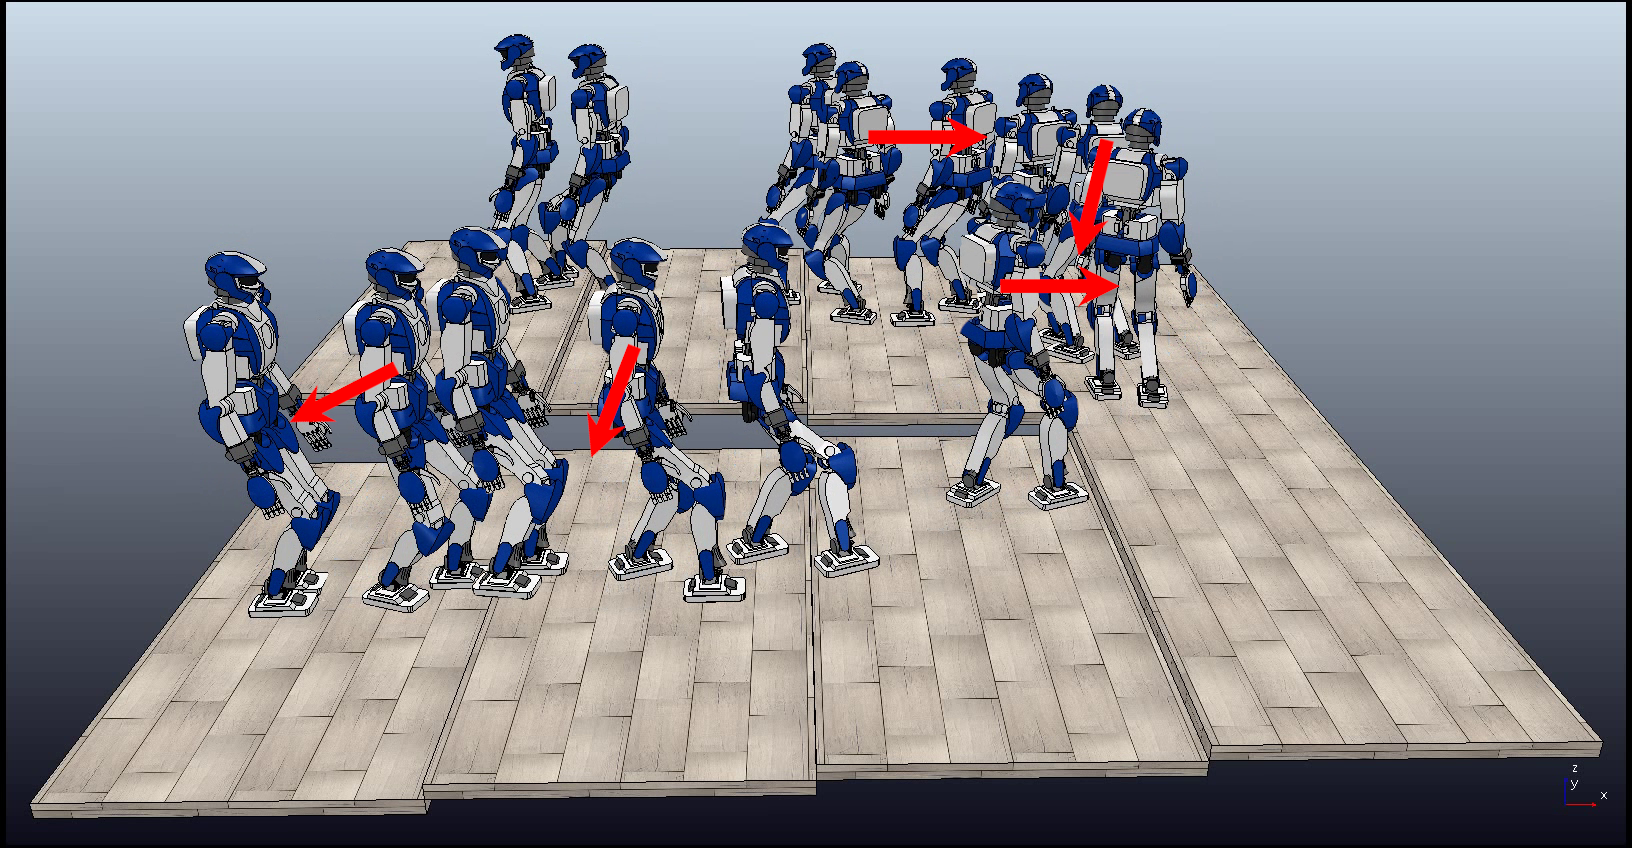
\includegraphics[trim={0.5cm 1.5cm 2cm 0.1cm},clip,width=0.9\columnwidth]{figures/strobo-staircase-with-pushes-2.png}
    \caption{An example simulation using the proposed architecture: the robot is walking along a staircase while being subject to multiple pushes. The adaptation module modifies position, orientation and timing of the footsteps real-time to guarantee a successful execution.}
    \label{fig:FAPA:two-patches-mixed-integer-snapshots}
\end{figure}

\section{Problem formulation} 
\label{sec:FAPA:ProblemFormulation}
The proposed architecture is shown in Fig.~\ref{fig:FAPA:block_scheme}.
An external candidate plan is provided, which in this chapter will be either
a basic plan to demonstrate simple motions, or a plan generated by randomized
exploration (Chapter \ref{ch:humanoid-motion-generation-WoS})
for more complex environments.
A subplan, i.e., a portion of the candidate plan, is given as input to the
scheme at each timestep.

\begin{figure}
    \centering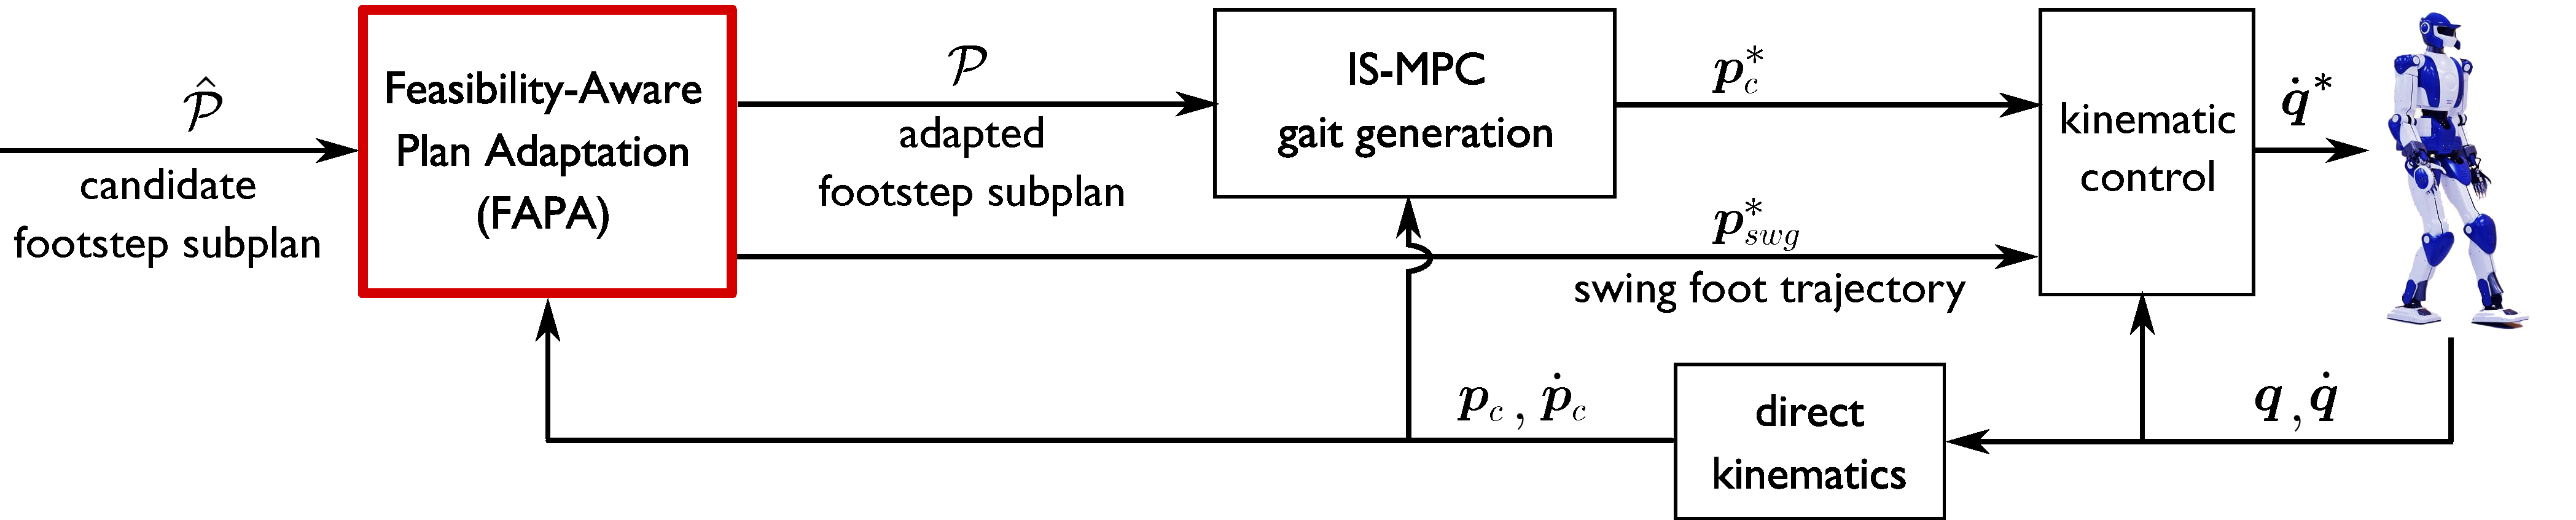
\includegraphics[width=\textwidth]{figures/BlockScheme-NLP-STA.pdf}
    \caption{A block scheme of the proposed architecture. The candidate footstep subplan $\mathcal{\hat{P}}$ is adapted by the FAPA module, guaranteeing the feasibility of IS-MPC. The IS-MPC module receives the adapted footstep subplan $\mathcal{P}$, and generates a desired trajectory of the CoM $\bm{p^*}_c$, which is used by the kinematic controller, together with the desired trajectory of the swing foot $\bm{p^*}_{\rm swg}$, to generate the desired joint velocities $\dot{\bm{q^*}}$.}
    \label{fig:FAPA:block_scheme}
    \end{figure}

The basic components of the considered scheme are:
\begin{itemize}
    \item a Feasibility-Aware Plan Adaptation (FAPA) block, that can modify locally
        the high-level footstep plan;
    \item an IS-MPC gait generation block (Chapter \ref{ch:ISMPC}) that generates CoM/ZMP trajectories based
        on the output of FAPA;
    \item a kinematic controller that realizes at the joint level the generated
        CoM and swing foot trajectories.
\end{itemize}

While the high-level footstep plan is designed considering the humanoid's
kinematic limitations, it is entirely unaware of its dynamics and is not
informed by the robot state since it is fully generated off-line.
To make up for this deficiency, the FAPA module performs a local adaptation of
the planned footsteps before these enter the IS-MPC stage. 

This adaptation is based on a {\em gait feasibility constraint} that guarantees
feasibility of the next IS-MPC stage while trying to match the original plan.
It can concurrently change the footstep positions, orientations, as well as
step timings. 

To formulate this constraint, we leverage the feasibility region of IS-MPC
(i.e., the subset of the state space where the problem is feasible at a given
time), and define it in an implicit form with the nonlinear dependency on the footstep
positions, orientations, and step timings.

The fact that the feasibility of the MPC can be efficiently captured by
the expression of this constraint is a crucial aspect of the formulation,
because it means that the scheme can harness the power of nonlinear
optimization without burdening the MPC itself, which remains linear and can
run at a high rate. The nonlinear optimization part is external to the MPC,
which allows the number of variables to be kept small and thus to keep the
computation time manageable.

We propose two versions of the FAPA module, that differ by the optimization
problem required for their implementation. In particular, the first version
only uses continuous optimization, while the second one also employs discrete
variables and is formulated as a Mixed Integer Nonlinear Program (MINLP).
Being the latter very general it can be used to account for more adaptation
scenarios, e.g., in which the footsteps can also be moved to different terrain
patches than the ones assigned by the high-level planner. As will be discussed
extensively in Sect.~\ref{sec:FAPA:Simulations}, the second version is more
demanding in terms of computation time, but we present it as a proof of
concept as we strongly believe it can be made to work in real time with proper
code optimization.

\section{Preliminaries}
\label{sec:FAPA:Preliminaries}
In this section we describe the environment and the structure of the footstep
plan used in our scheme.

\subsection{Environment}
The considered environment is a world of stairs, i.e., constituted by flat
horizontal regions. The robot is allowed to walk across different regions if
these are relatively close in height, and if there is sufficient available
surface to step on them, otherwise they will constitute obstacles to be avoided.

The arrangement of these regions is assumed to be known, and it is processed
and encoded in the following way:
\begin{itemize}
    \item regions are reduced in size so that they represent the collision-free
        area available for the center of the footprint. This is done by
        performing a Minkowski difference between each flat region and the
        area swept by a footprint (accounting for all possible footstep orientations);
    \item after reduction, non-convex regions are subdivided into
        non-overlapping convex polytopic {\em patches}.
\end{itemize}
A patch $P$ is identified by the inequality $\bfA(P) \bfp \le \bfb(P)$,
where $\bm{A}(P) \in \mathbb{R}^{V(P) \times 2}$ and
$\bm{b}(P) \in \mathbb{R}^{V(P)} $ define a polytope (with $V(P)$ vertices)
and $\bfp = (x, y)^T$ is a generic 2D point. 
In this way, non-polytopic portions of ground (e.g., round edges) are
approximated, but the number of vertices can be arbitrarily large.
Since each patch $P$ is flat, its height is denoted simply as $z(P)$.

\subsection{Footstep plan}
The high-level footstep plan is a sequence of {\em candidate footsteps}
$\hat\bff$, each identified by the tuple
$\hat\bff = (\hat x_f, \hat y_f, \hat z_f, \hat\theta_f, \hat T_{\rm ss}, \hat T_{\rm ds})$.
For each planned footstep $\hat\bff$

\begin{itemize}
    \item $\hat x_f$, $\hat y_f$ and $\hat z_f$ are the coordinates of its center;
    \item $\hat\theta_f$ is its orientation around the $z$ axis;
    \item $\hat T_{\rm ds}$ and $\hat T_{\rm ss}$ are the durations of its  double support and single support phases, respectively;
    \item we denote by $\Pi(\hat\bff)$ the patch that contains the footstep, i.e., the patch $P$ such that\footnote{Note that this patch is unique because the environment is subdivided into non-overlapping patches.}
    \[
    (\hat{x}_f, \hat{y}_f)^T \in P,\quad \hat{z}_f = z(P).
    \]
\end{itemize}

The footstep plan $\mathcal{\hat P}$ is computed off-line, and at each time
$t_k$ a subplan $\mathcal{\hat P}^l$ of size $F+1$ is extracted, where $l$ is
the index of the first footstep of the current subplan (at $t_k$), and $F$ a
fixed parameter. The subplan contains the next $F$ candidate footsteps:
\begin{equation*}
\mathcal{\hat P}^l = \left\{
\hat\bff^{l},\,\dots,\,\hat\bff^{l+F}
\right\}.
\end{equation*}
The FAPA block, which performs footsteps adaptation, modifies
$\mathcal{\hat P}^l$ in the adapted subplan $\mathcal{P}^l$, i.e., in the input
of the IS-MPC block
\begin{equation*}
    \mathcal{P}^l = \left\{
    \bff^{l},\,\dots,\,\bff^{l+F}
    \right\}.
\end{equation*}

After every iteration, if adaptation took place (i.e., $\mathcal{P}^l$ differs
from $\mathcal{\hat P}^l$), the algorithm performs a {\em footstep plan
override}, i.e., the corresponding portion of the high-level footstep plan
is substituted with the adapted subplan $\mathcal{P}^l$. Note that the
remaining part of the plan (after the index $l+F$) is unchanged, so if the
adaptation makes the robot stray from the initial path it will later try to
catch up. This behavior is often acceptable, but might sometimes be undesirable,
and can be improved in future versions if we allow the high-level planner
to replan on-line (see \cite{Cipriano2023RAS}).

\section{Feasibility-Aware Plan Adaptation}
\label{sec:FAPA:FeasibilityAwarePlanAdaptation}

\textbf{From Humanoids 2023 Feasibility region section:} In the following
section, we will describe how to use the feasibility region to formulate a
constraint for the FAPA module, and thus ensure that the output of FAPA can be
used by IS-MPC to construct a feasible QP.

The FAPA module runs in real-time and performs a local adaptation of the
subplan $\mathcal{\hat P}^l$, including their timing. We now describe the
constraints and the optimization problems that define the adaptation procedure.

\subsection{Kinematic constraint}

\begin{figure}
    \centering
    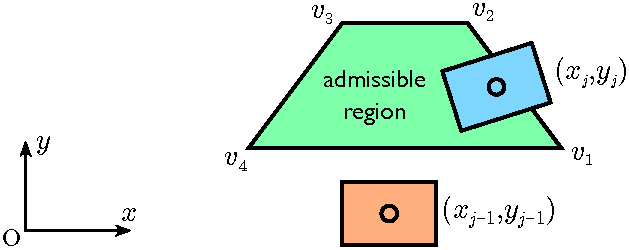
\includegraphics[width=0.7\textwidth]{figures/humanoids_kinconstr.pdf}
    \caption{Admissible region of the kinematic constraint in the $x$-$y$ plane.}
    \label{fig:FAPA:kinematic-constraint}
\end{figure}

The $j$-th footstep $\bff^{j}$ is ensured to be kinematically feasible by
limiting its displacement with respect to the previous footstep $\bff^{j-1}$.
In practice we constrain the geometric components of $\bff^{j}$ to be within
the \textit{admissible region}
\begin{equation}
\label{eq:FAPA:kinematic-constraint}
\begin{split}
\begin{pmatrix}
    \bm{n}_1^T\left(\bm{p}_{xy}^{l+j} - \bm{p}_{xy}^{l+j-1} - \bm{R}(\theta_f^{l+j-1})\bm{v}_1\right) \\
    \vdots \\
    \bm{n}_V^T\left(\bm{p}_{xy}^{l+j} - \bm{p}_{xy}^{l+j-1} - \bm{R}(\theta_f^{l+j-1})\bm{v}_V\right) \\
\end{pmatrix} \ge \bm{0},\\
    \Delta z^{\rm m} \le z_{l+j} - z_{l+j-1} \le \Delta z^{\rm M}, \\
    \Delta \theta^{\rm m} \le \theta_{l+j} - \theta_{l+j-1} \le \Delta \theta^{\rm M}, 
\end{split}
\end{equation}
with $\bm{R}(\theta_f^{l+j-1})$ a 2D rotation matrix, $\bm{n}_i$ the vector
normal to the $i$-th segment of the convex region computed as
\begin{equation*}
    \bm{n}_i =
    \begin{pmatrix}
        0 & -1 \\ 1 & 0
    \end{pmatrix}
    \bm{R}(\theta_f^{l+j-1})(\bm{v}_{i+1}-\bm{v}_i),
\end{equation*}
and $\bm{v}_i$ being the vertices defining the convex polygon (different
depending whether the support foot is left or right), shown in
Fig. \ref{fig:FAPA:kinematic-constraint}. Furthermore,
$\Delta_z^m$, $\Delta z^{\rm M}$, $\Delta \theta^{\rm m}$, and
$\Delta \theta^{\rm M}$ define limits for the foot reachability over vertical
displacement and relative orientation.

\subsection{Timing constraint}
Single and double support duration are subject to minimum and maximum duration
constraints
\begin{equation}
    T_{\rm ds}^{\min} \le T_{\rm ss}^{l+j} \le T_{\rm ds}^{\max}, \quad T_{\rm ss}^{\min} \le T_{\rm ds}^{l+j} \le T_{\rm ss}^{\max},
    \label{eq:FAPA:timing-constraint}
\end{equation}
where the bounds $T_{\rm ds}^{\min}$, $T_{\rm ds}^{\max}$, $T_{\rm ss}^{\min}$, $T_{\rm ss}^{\max}$ are chosen in such a way to avoid excessively fast trajectories that might be difficult to track, as well as very slow steps that could result in quasi-static motion.

\subsection{Patch constraints}
\label{sec:FAPA:patch_constraint}
We describe alternative versions of this constraint, as we will later compare
the module using either of them, both in terms of the quality of the resulting
plan and of the computational load.
The first version of the constraint simply restrict the $(l+j)$-th footstep
to lie within its associated patch $\Pi(\bff^{l+j})$, which is the one
originally chosen by the high-level planner. This constraint can be written as
\begin{equation}
    \begin{cases}
		\bm{A}(\Pi(\bff^{l+j})) \left( x_f^{l+j} \ y_f^{l+j} \right)^T \leq \bm{b}(\Pi(\bff^{l+j})), \\
		z_f^{l+j} = z(\Pi(\bff^{l+j})).
    \end{cases}
	\label{eq:FAPA:fixed_patch_constraint}
\end{equation}

The second version of the patch constraint allows the footstep to be moved
to a different patch. To entertain this possibility, we introduce binary
variables in order to formulate a mixed-integer constraint. This constraint
defines a logical implication in which, if a certain binary variable
$b_{l+j,\kappa}$ is {\em true}, then a linear constraint must be verified:
\begin{equation}
	b_{l+j,\kappa}=1 \Rightarrow 
	\begin{cases}
		\bm{A}(P^\kappa) \left( x_f^{l+j} \ y_f^{l+j} \right)^T \leq \bm{b}(P^\kappa), \\
		z_f^{l+j} = z(P^\kappa).
	\end{cases}
	\label{eq:FAPA:implication}
\end{equation}
This forces the $(l+j)$-th footstep to lie within the $\kappa$-th patch.
Since each footstep can only be inside a single patch, we also impose
\begin{equation}
    \sum^R_{\kappa=1} b_{l+j,\kappa} = 1.
    \label{eq:FAPA:sum_one}
\end{equation}

In MIP, logical implications can be implemented using binary variables through
the so-called {\em big-M} technique
\cite{Afonso2020TaskAllocationTrajectoryPlanning}. In this case, we rewrite
\eqref{eq:FAPA:implication} as
\begin{equation}
	\begin{cases}
		\bm{A}(P^\kappa)\left( x_f^{l+j} \ y_f^{l+j} \right)^T \leq \bm{b}(P^\kappa) + (1 - b_{l+j,\kappa}) M \bm{1}_{V(P^\kappa)}, \\
		z_{l+j} \leq z(P^\kappa) + (1 - b_{l+j,\kappa}) M, \\
		-z_{l+j} \leq -z(P^\kappa) + (1 - b_{l+j,\kappa}) M,
	\end{cases}
\label{eq:FAPA:mi_patch_constraint}
\end{equation}
where $M$ is a constant large enough to relax the constraints if
$b_{l+j,\kappa}=0$ and $\bm{1}_{V(P^\kappa)}$ is a row vector with
$V(P^\kappa)$ ones. We define $\hat \kappa_{l+j}$ as the index of
$\Pi(\hat \bff^{l+j})$. Note that this requires turning the equality constraint
into two inequality constraints. Based on the patches of the candidate footsteps
in $\mathcal{\hat P}^l$, we also define candidate binary variables as
\begin{equation*}
    \hat b_{l+j,\kappa} =
    \begin{cases}
        1, \ \text{if } \kappa = \hat \kappa_{l+j}, \\
        0, \ \text{if } \kappa \neq \hat \kappa_{l+j}.
    \end{cases}
\end{equation*}
Finally, \eqref{eq:FAPA:sum_one} and \eqref{eq:FAPA:mi_patch_constraint}
assume that every footstep may be mapped to every patch, which requires
$F \times R$ binary variables. However, since the computational load of a
MIP is largely related to the number of binary variables, we employ a heuristic
that allows a footstep $\bff^j$ to be assigned only to the patches adjacent to
$\Pi(\hat \bff^j)$.

\subsection{Current footstep constraints}

The first footstep in the subplan $\bff^l$ corresponds to the footstep
currently in contact with the ground, which means that some of its components
cannot be changed. In particular, its geometric components should be
constrained to be equal to the corresponding components of $\hat\bff^l$, i.e.,
\begin{equation}
    x_f^l = \hat x_f^l, \quad
    y_f^l = \hat y_f^l, \quad
    z_f^l = \hat z_f^l, \quad
    \theta_f^l = \hat \theta_f^l.
    \label{eq:FAPA:current_geometric_constraint}
\end{equation}
Note that, because of the footstep plan override, the components of
$\hat\bff^l$ are not the same as in the original plan, but rather those
adapted at the previous iteration.

If $t_k$ belongs to a single support phase, the double support of the current
step cannot be changed anymore because it is already passed. This is expressed
by the constraint
\begin{equation}
	t_k - t_s^l > T^l_{\rm{ds}} \quad \Rightarrow \quad  T^l_{\rm{ds}} = \hat T^l_{\rm{ds}}.
	\label{eq:FAPA:double_support_decided}
\end{equation}
Note that the implication in \eqref{eq:FAPA:double_support_decided} is handled
at the code level and does not require introducing binary variables.

To avoid footstep changes when the swing foot is close to touching the ground,
when nearing the end we add the following constraint:
\begin{equation}
    \label{eq:FAPA:swing_foot_constraint}
	T^l_{\rm ds} + T^l_{\rm ss} - t_k + t_s^l < t_{\mathrm{change}} \quad \Rightarrow \quad
	\bff^{l+1} = \hat\bff^{l+1}.
\end{equation}

\subsection{Gait feasibility constraints}
The gait feasibility constraints are introduced to ensure that IS-MPC is
feasible. They do so by constraining the current state to be within the
feasibility region \eqref{eq:FAPA:mpc-feasibility-constraint}.

The expression of the feasibility region
\eqref{eq:FAPA:mpc-feasibility-constraint} uses the ZMP bounds, that clearly
depend on the motion of the moving box, and thus on the footsteps positions
and timings. To derive a constraint, we simply make this dependency explicit
by plugging \eqref{eq:FAPA:zmp_constraint_displacement} and
\eqref{eq:FAPA:mapping} inside \eqref{eq:FAPA:mpc-feasibility-constraint}.
Focusing on the right inequality of the $x$ component, this results in
\begin{equation}
    \label{eq:FAPA:gait_feasibility_constraint}
    x_u^k + b_x^k \le \bm{s}^T \bm{Z}^{-1} \left(\bfM\bfX_f^l + \bfm x_f^l + \bm{z} \left(\frac{d_x}{2} - x_z^k\right)\right).
\end{equation}
The $y$ and $z$ components, as well as the left inequalities result in
analogous expressions, which we omit for space concerns.

\subsection{Feasibility-driven plan adaptation algorithm}
We present two different versions of the FAPA algorithm. The first one is not
allowed to move footsteps from a different patch to the one in the original
plan, and is thus referred to as Fixed patches FAPA (F-FAPA). The second one
is instead allowed to choose different patches, and goes under the name of
Variables patches FAPA (V-FAPA).

The decision variable over the planning horizon are collected as
% per recuperare spazio anche se c'è overfull ....
\begin{align*}
    \bfX_f^l & =  (x_f^l,\dots,x_f^{l+F}), \quad 
    \,\, \bfY_f^l  =  (y_f^l,\dots,y_f^{l+F}), \\
    \,\, \bfZ_f^l & = (z_f^l,\dots,z_f^{l+F}), \quad
    \bm{\Theta}_f^l = (\theta_f^l,\dots,\theta_f^{l+F}), \\
    \,\, \bfT_{\rm ds}^l & =  (T_{\rm ds}^l,\dots,T_{\rm ds}^{l+F}), \quad \bfT_{\rm ss}^l \!=\! (T_{\rm ss}^l,\dots,T_{\rm ss}^{l+F}), 
\end{align*}
\begin{equation*}
\bfB^l = \left(
\begin{array}{ccc}b_{l,1} & \dots & b_{l,L}\\ \vdots & \ddots & \vdots \\ b_{l+F,1} & \dots & b_{l+F,L} \end{array}
\right),
\end{equation*}
while the corresponding candidate values are identified by the vectors
$\hat \bfX_f^l$, $\hat \bfY_f^l$, $\hat \bfZ_f^l$, $\hat {\bm{\Theta}}_f^l$, $\hat \bfT^l_{\rm ds}$, $\hat \bfT^l_{\rm ss}$, $\hat \bfB^l$, similarly defined.

F-FAPA solves the following problem, with decision variables
$\bfU^l = (\bm{X}_f^l, \bm{Y}_f^l, \bm{Z}_f^l, \bm{\Theta}_f^l, \bm{T}_{\rm ds}^l, \bm{T}_{\rm ss}^l)$:
\begin{braced}
    \begin{equation*}
        \begin{split}
            \min_{\bfU^l}\quad
            & w_x \| \hat{\bm{X}}_f^l - \bm{X}_f^l \|^2 + w_y \| \hat{\bm{Y}}_f^l - \bm{Y}_f^l \|^2 + \\& w_z \| \hat{\bm{Z}}_f^l - \bm{Z}_f^l \|^2 + w_{\theta} \| \hat{\bm{\Theta}}_f^l - \bm{\Theta}_f^l \|^2 + \\& w_{\rm ds} \| \hat{\bm{T}}_{\rm ds}^l - \bm{T}_{\rm ds}^l \|^2 + w_{\rm ss} \| \hat{\bm{T}}_{\rm ss}^l - \bm{T}_{\rm ss}^l \|^2
        \end{split}
    \end{equation*}
    \hspace{0.25cm} subject to:
    \begin{itemize}
        \item kinematic constraints \eqref{eq:FAPA:kinematic-constraint}, for $j=1,\dots,F$
        \item timing constraints \eqref{eq:FAPA:timing-constraint}, for $j=0,\dots,F$
        \item fixed patch constraints \eqref{eq:FAPA:fixed_patch_constraint}, for $j=1,\dots,F$
        \item current footsteps constraints \eqref{eq:FAPA:current_geometric_constraint}, \eqref{eq:FAPA:double_support_decided} and \eqref{eq:FAPA:swing_foot_constraint}
        \item gait feasibility constraints \eqref{eq:FAPA:gait_feasibility_constraint}
    \end{itemize}
\end{braced}

\medskip

Since F-FAPA does not have binary variables, it can be implemented using a
regular nonlinear solver (i.e., \texttt{ipopt}).

V-FAPA solves the following problem, with decision variables which now include
the binary variables $\bm{B}^{l}$ that is $\bfW^l = (\bm{X}_f^l, \bm{Y}_f^l, \bm{Z}_f^l, \bm{\Theta}_f^l, \bm{T}_{\rm ds}^l, \bm{T}_{\rm ss}^l, \bm{B}^{l})$:
\begin{braced}
    \begin{equation*}
        \begin{split}
            \min_{\bfW^l} \quad
            & w_x \| \hat{\bm{X}}_f^l - \bm{X}_f^l \|_2^2 + w_y \| \hat{\bm{Y}}_f^l - \bm{Y}_f^l \|_2^2 + \\& w_z \| \hat{\bm{Z}}_f^l - \bm{Z}_f^l \|_2^2 + w_{\theta} \| \hat{\bm{\Theta}}_f^l - \bm{\Theta}_f^l \|_2^2 + \\& w_{\rm ds} \| \hat{\bm{T}}_{\rm ds}^l - \bm{T}_{\rm ds}^l \|_2^2 + w_{\rm ss} \| \hat{\bm{T}}_{\rm ss}^l - \bm{T}_{\rm ss}^l \|_2^2 +  \\&
            w_{\rm b} \| \hat{\bm{B}}^l - \bm{B}^l \|_2^2
        \end{split}
    \end{equation*}
    \hspace{0.25cm} subject to:
    \begin{itemize}
        \item kinematic constraints \eqref{eq:FAPA:kinematic-constraint}, for $j=1,\dots,F$
        \item timing constraints \eqref{eq:FAPA:timing-constraint}, for $j=0,\dots,F$
        \item variable patch constraints \eqref{eq:FAPA:sum_one} and \eqref{eq:FAPA:mi_patch_constraint}, for $j=1,\dots,F$
        \item current footsteps constraints \eqref{eq:FAPA:current_geometric_constraint}, \eqref{eq:FAPA:double_support_decided} and \eqref{eq:FAPA:swing_foot_constraint}
        \item gait feasibility constraints \eqref{eq:FAPA:gait_feasibility_constraint}
    \end{itemize}
\end{braced}

\medskip

Since V-FAPA contains the binary variables $\bm{B}$ it is implemented as a MINLP.

\section{Simulations}
\label{sec:FAPA:Simulations}
We ran four simulations in MATLAB, using CoppeliaSim to kinematically
visualize the resulting motions. The system is an AMD Ryzen 9 5900X
(4.8 GHz, 12 core) with 16 GB DDR4 3600 MHz running Ubuntu 22.04 LTS. IS-MPC
runs at 100~Hz and is solved using \texttt{quadprog}, while FAPA runs at
10~Hz and is solved using the CasADi interface. In CasADi, we used
\texttt{ipopt} for F-FAPA, and \texttt{bonmin} for V-FAPA. We also ran tests
with the commercial solver \texttt{knitro}, to compare the performance
(see Table~\ref{tab:benchmarks}).

All the simulations use the parameters of Table \ref{tab:FAPA:hyperparameters}.
Simulation videos are available at \url{https://youtu.be/4_QYsZH1E7Y}.

\begin{table}
    \centering
    \begin{tabular}{ |c|c| } 
        \hline
        Symbol & Value \\
        \hline
        $\delta$ & 0.01 [s] \\
        $T_c$ & 2.0 [s] \\
        $T_p$ & 4.0 [s] \\
        $\eta$ & 3.6 [s$^{-1}$] \\
        $\beta$ & 100 \\
        $d_x, d_y, d_z$ & 0.035 [m] \\
        $F$ & 3 \\
        $\bm{v}_1$ & $(0.28, 0.13)^T $ [m] \\
        $\bm{v}_2$ & $(0.2, 0.43)^T$ [m] \\
        $\bm{v}_3$ & $(-0.12, 0.43)^T$ [m] \\
        $\bm{v}_4$ & $(-0.2, 0.13)^T$ [m] \\
        $\Delta_z^m$ & -0.10 [m] \\
        $\Delta_z^M$ & 0.10 [m] \\
        $\Delta_{\theta}^m$ & -0.4 [rad] \\
        $\Delta_{\theta}^M$ & 0.4 [rad] \\
        $T_{\rm ds}^{\min}$ & 0.3 [s] \\
        $T_{\rm ds}^{\max}$ & 0.5 [s] \\
        $T_{\rm ss}^{\min}$ & 0.5 [s] \\
        $T_{\rm ss}^{\max}$ & 0.7 [s] \\
        $t_{\rm change}$ & 0.1 [s] \\
        $M$ & 100 \\
        $w_x, w_y, w_z, w_{\theta}$ & 1.0 \\
        $w_{\rm ds}, w_{\rm ss}$ & 1.0 \\
        $w_b$ & 0.01 \\
        \hline
    \end{tabular}
    \caption{Hyperparameters of F-FAPA and V-FAPA used in all the experiments.}
    \label{tab:FAPA:hyperparameters}
\end{table}

Simulations take place in 3 different scenarios: {\em empty}, which is
completely flat with no obstacles, and is represented using a single patch;
{\em 2-patches} is constituted by two patches at different heights
(0 and 0.06~m); {\em stairs} has a total of 7 patches of increasing height.
While walking, the robot is subject to impulsive pushes (lasting 0.01~s),
transformed in equivalent acceleration imparted on the CoM.

In the first simulation, the robot is walking forward in the {\em empty}
scenario. At 4.5~s it receives a 15.6~m/s$^2$ push in the direction $(-2, -1, 0)$,
that without FAPA would make the MPC infeasible. F-FAPA reacts by adapting
footstep positions, orientations and timings concurrently, allowing the MPC
to recover feasibility. Figure \ref{fig:FAPA:matlab_empty} shows nominal and
adapted footsteps, trajectories and step timings.
Figure \ref{fig:FAPA:sim1:snapshots} shows a sequence of snapshots of the
HRP-4 humanoid robot executing the motion.
\begin{figure}
    %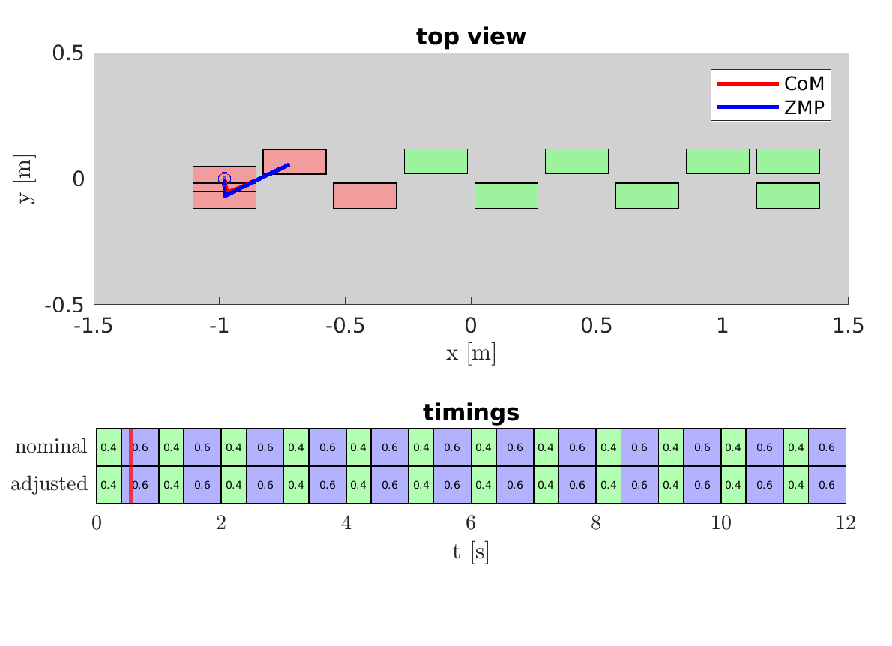
\includegraphics[trim={0 1cm 0 0},clip,width=\textwidth]{figures/empty-fixed-plot-starting.pdf}
    \centering
    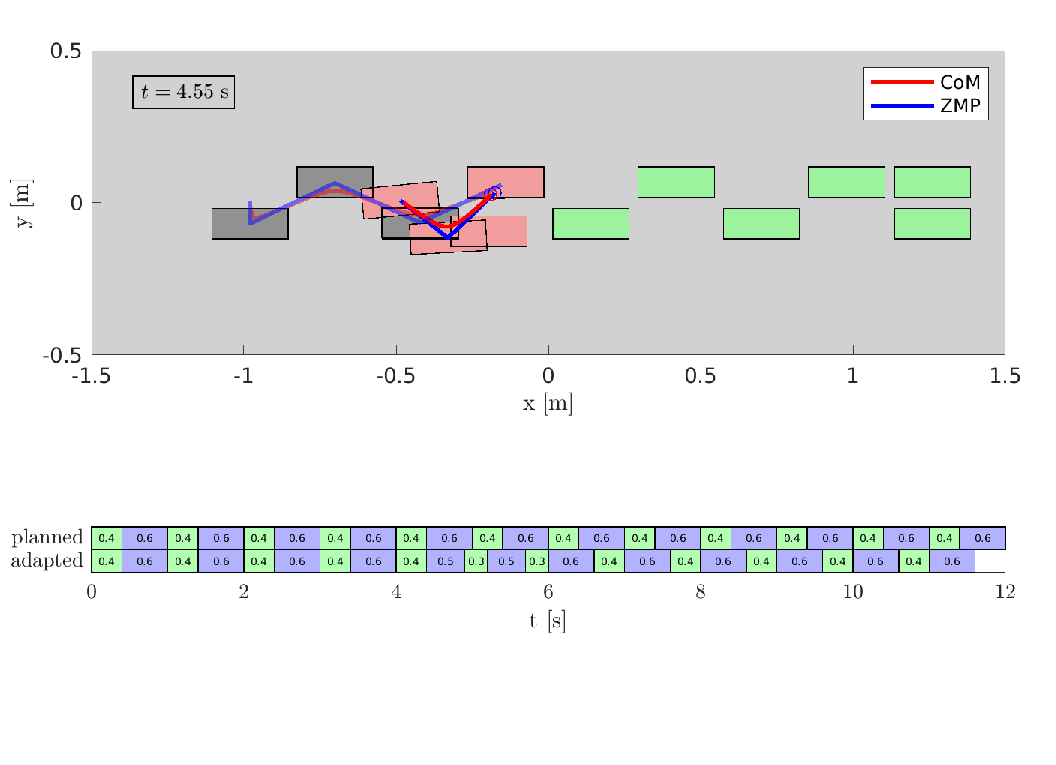
\includegraphics[trim={0 5.9cm 0 0.7cm},clip,width=\textwidth]{figures/empty-fixed-plot-after-push.pdf}
    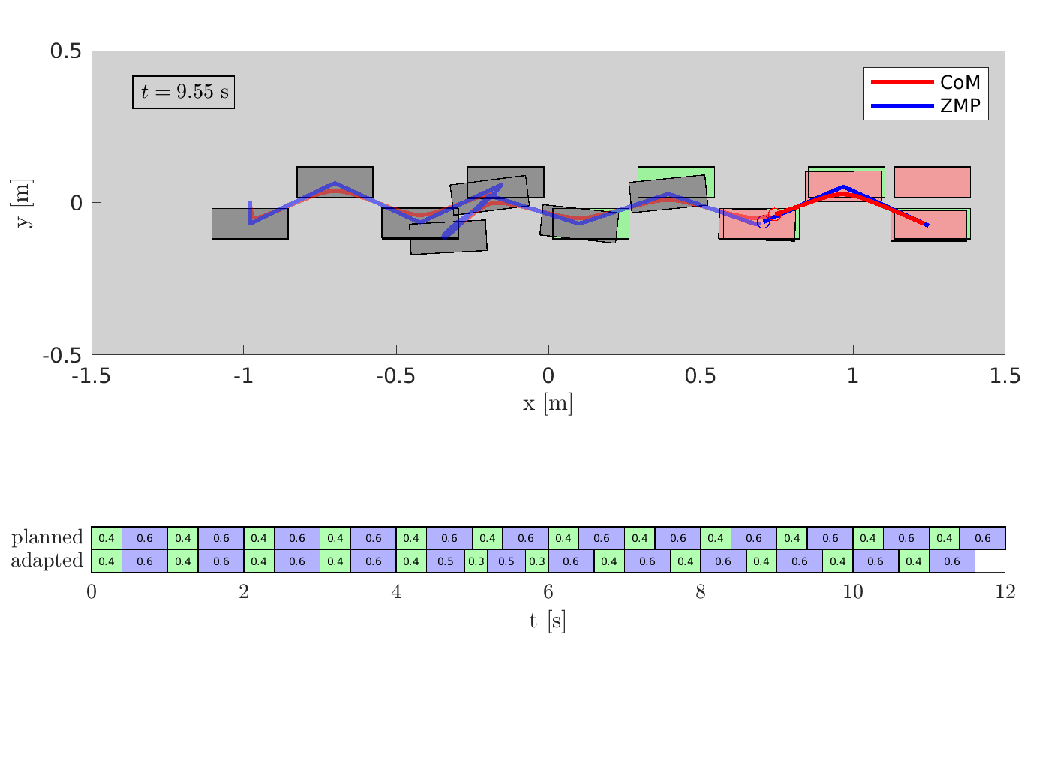
\includegraphics[trim={0 5.9cm 0 0.7cm},clip,width=\textwidth]{figures/empty-fixed-plot-completing-task.pdf}
    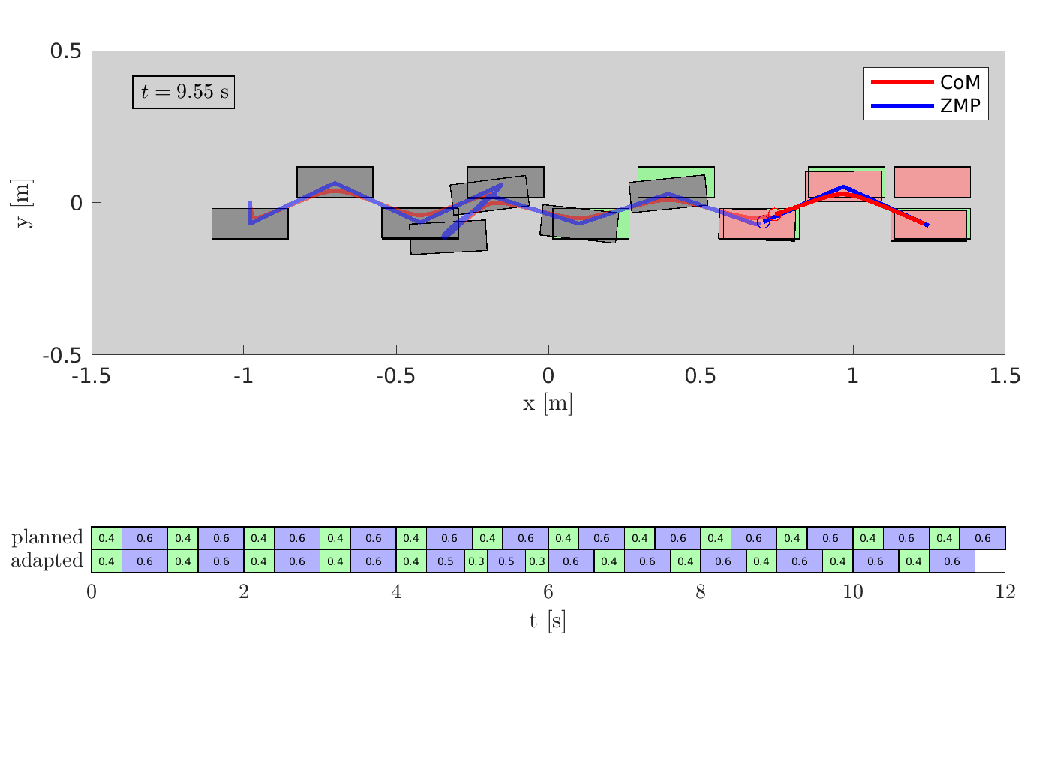
\includegraphics[trim={0 2.2cm 0 8.6cm},clip,width=\textwidth]{figures/empty-fixed-plot-completing-task.pdf}
    \caption{F-FAPA in the {\em empty} scenario. The robot is walking in a
        straight line and is pushed at time $4.5$~s (slightly before the first
        snapshot). Green footsteps represent the original candidate plan, while
        the footsteps that are actually executed are shown in grey. Red
        footsteps represent the current adapted subplan. The two bands on the
        bottom show the nominal and adapted timings (green for double support
        and blue for single support). The same color scheme is used for the
        rest of the figures.
    }
    \label{fig:FAPA:matlab_empty}
\end{figure}

\begin{figure}
    \centering
    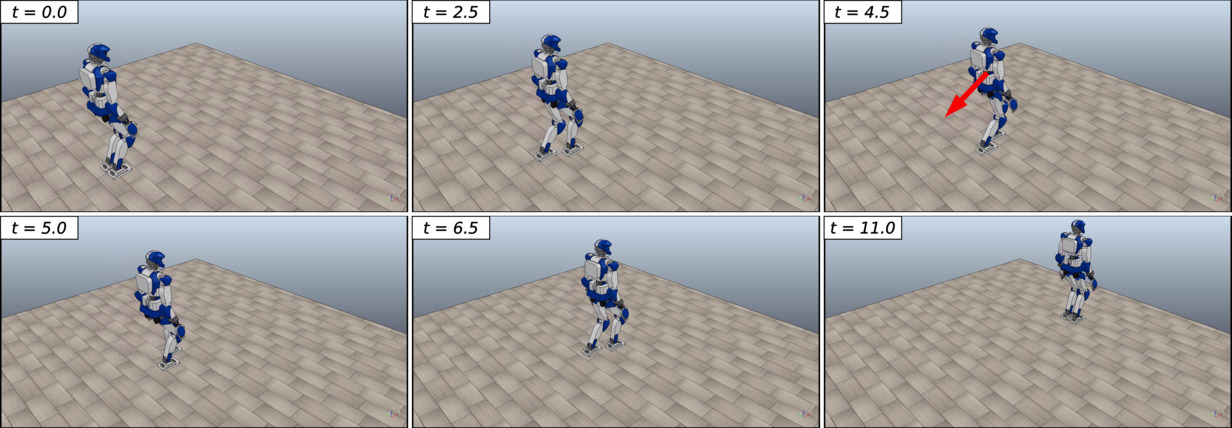
\includegraphics[width=\textwidth]{figures/empty-push-fixed-snapshots.jpeg}
    \caption{HRP-4 walking in the \textit{empty} scenario using F-FAPA.
        The robot walks in a straight line and it is pushed at time 4.5 s
        (third snapshot). The robot is able to sustain the push adapting the
        footsteps and the duration of single and double support
        (fourth snapshot), eventually reaching its desired goal (last snapshot).
    }
    \label{fig:FAPA:sim1:snapshots}
\end{figure}

In the second simulation (shown in Fig.~\ref{fig:FAPA:matlab_2pacf}), the scenario is {\em 2-patches}, and the robot must climb a step. Upon receiving the push, the footsteps do not change significantly, because the F-FAPA algorithm is not allowed to move the footstep to the other patch. As a result, the tolerable push is smaller, i.e., 7.8~m/s$^2$. Figure \ref{fig:FAPA:sim2:snapshots} shows a sequence of snapshots of the HRP-4 humanoid robot executing the motion.
\begin{figure}
    %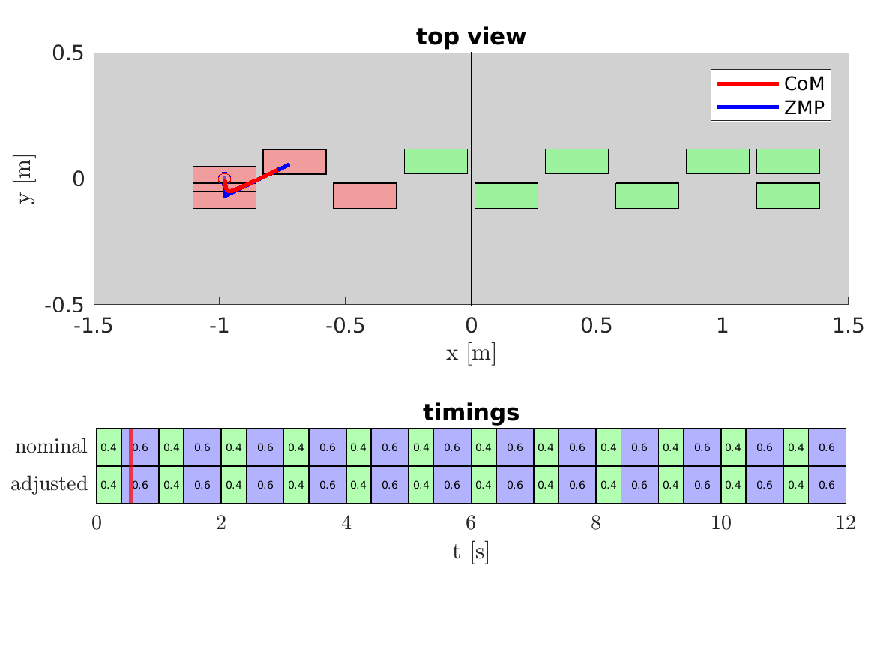
\includegraphics[trim={0 1cm 0 0},clip,width=\textwidth]{figures/two-patches-fixed-plot-starting.pdf}
    \centering
    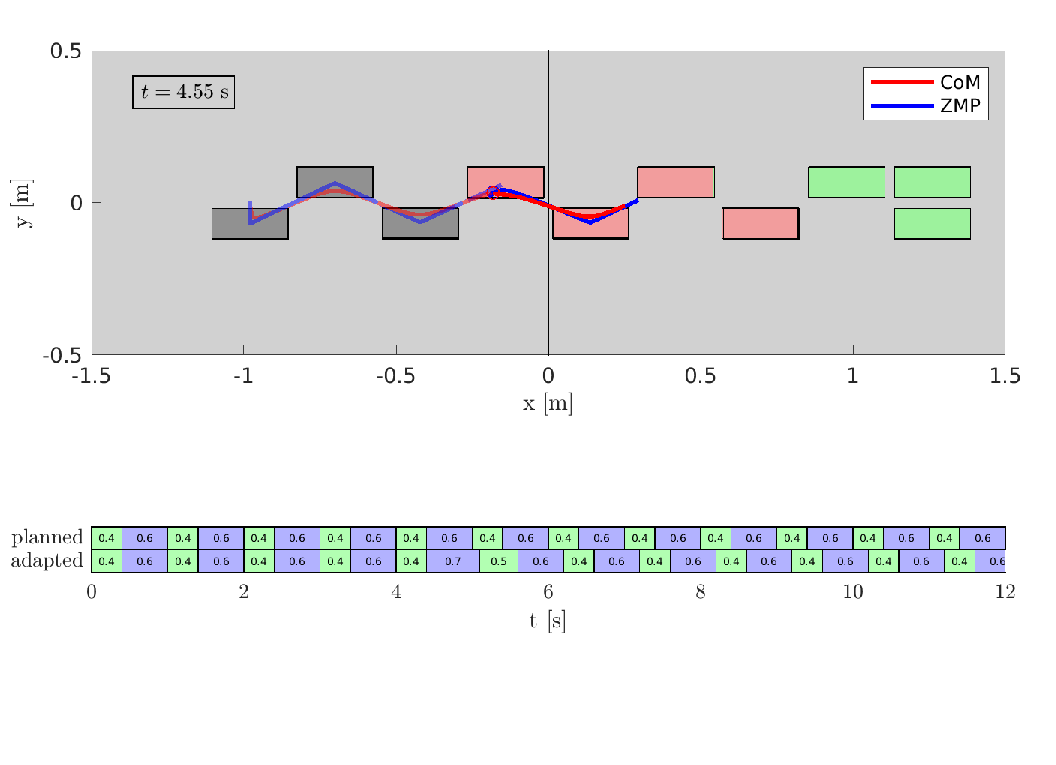
\includegraphics[trim={0 5.9cm 0 0.7cm},clip,width=\textwidth]{figures/two-patches-fixed-plot-after-push.pdf}
    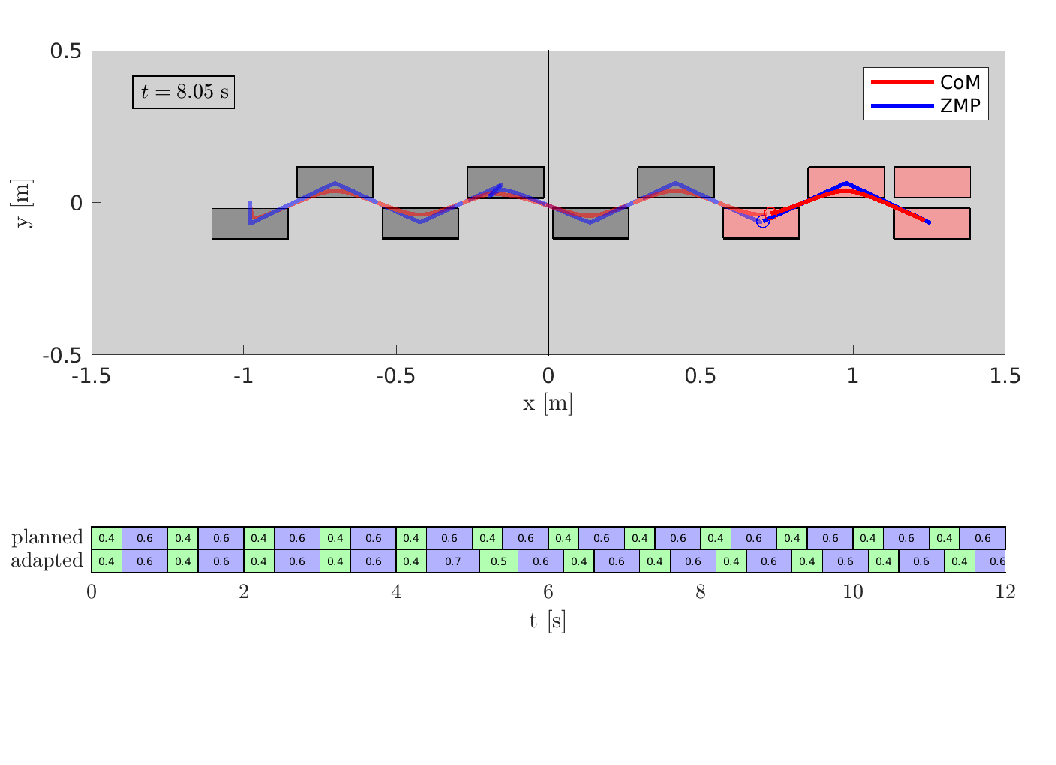
\includegraphics[trim={0 5.9cm 0 0.7cm},clip,width=\textwidth]{figures/two-patches-fixed-completing-task.pdf}
    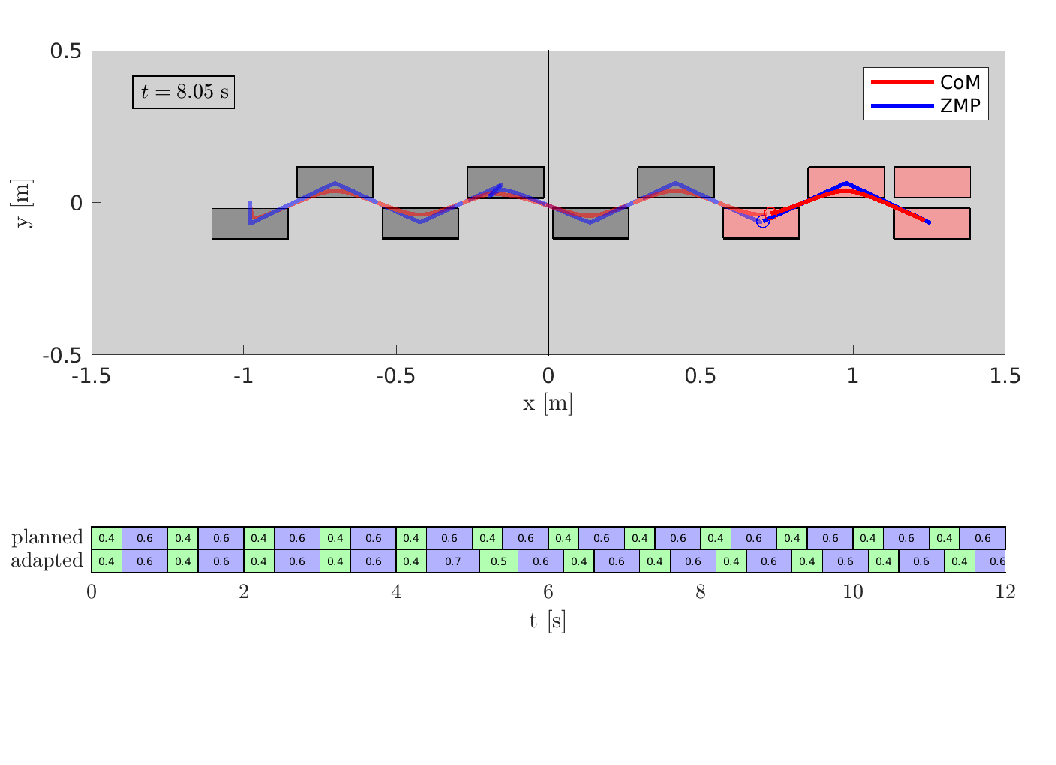
\includegraphics[trim={0 2.2cm 0 8.6cm},clip,width=\textwidth]{figures/two-patches-fixed-completing-task.pdf}
    \caption{F-FAPA in the {\em 2-patches} scenario. The robot is walking in
        a straight line and is pushed at time $4.5$~s (slightly before the
        first snapshot). Since changing patches is not allowed, the magnitude
        of the push that can be tolerated is quite small, compared to that of
        the other simulations.
    }
    \label{fig:FAPA:matlab_2pacf}
\end{figure}

\begin{figure}
    \centering
    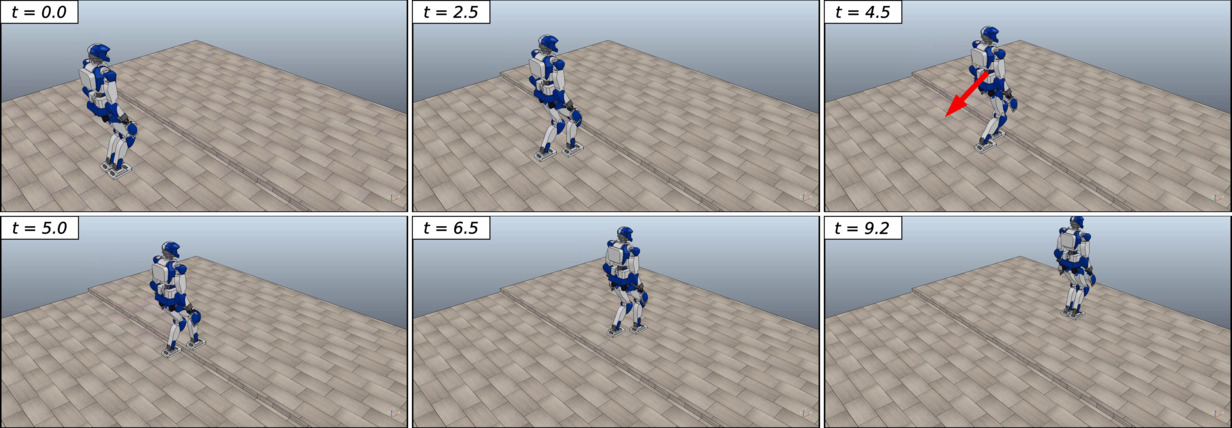
\includegraphics[width=\textwidth]{figures/two-patches-push-fixed-snapshots.jpeg}
    \caption{HRP-4 walking in the \textit{2-patches} scenario using F-FAPA. The robot walks in a straight line and it is pushed at time 4.5 s (third snapshot). The robot is able to sustain the push adapting the duration of single and double support (fourth snapshot), eventually reaching its desired goal (last snapshot).}
    \label{fig:FAPA:sim2:snapshots}
\end{figure}

In the third simulation (shown in Fig.~\ref{fig:FAPA:matlab_2pacmi} ), the scenario is still {\em 2-patches}, but now the scheme is using V-FAPA. When the push is perceived, the first predicted footstep is moved to the lower patch, and as a result the increase of the tolerable push intensity is very significant, i.e., the same as in the {\em empty} scenario.  Figure \ref{fig:FAPA:sim3:snapshots} shows a sequence of snapshots of the HRP-4 humanoid robot executing the motion.
\begin{figure}
    %\includegraphics[trim={0 1cm 0 0},clip,width=\textwidth]{figures/two-patches-mixed-integer-plot-starting.pdf}
    \centering
    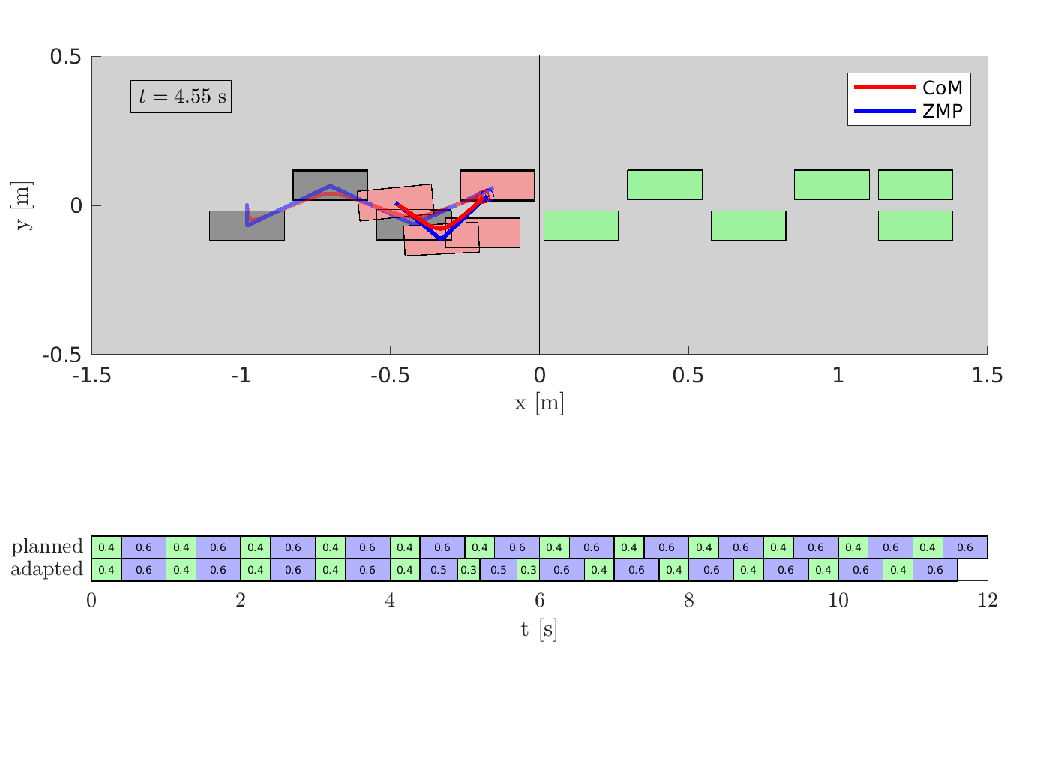
\includegraphics[trim={0 5.9cm 0 0.7cm},clip,width=\textwidth]{figures/two-patches-mixed-integer-after-push.pdf}
    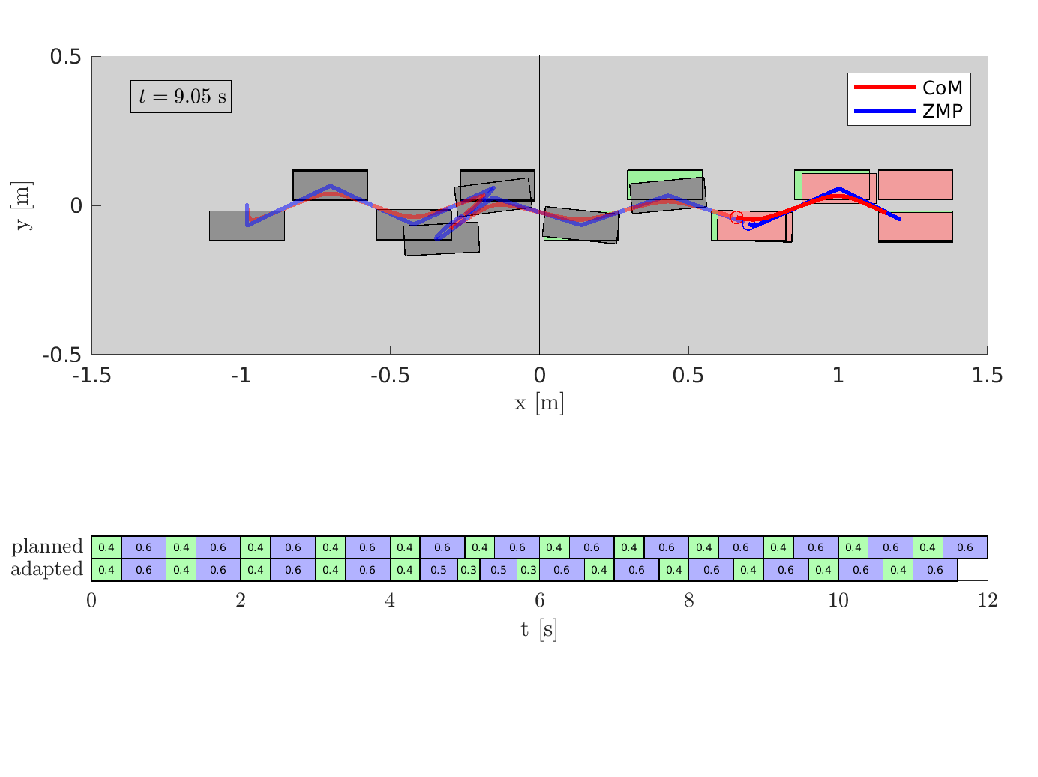
\includegraphics[trim={0 5.9cm 0 0.7cm},clip,width=\textwidth]{figures/two-patches-mixed-integer-completing-task.pdf}
    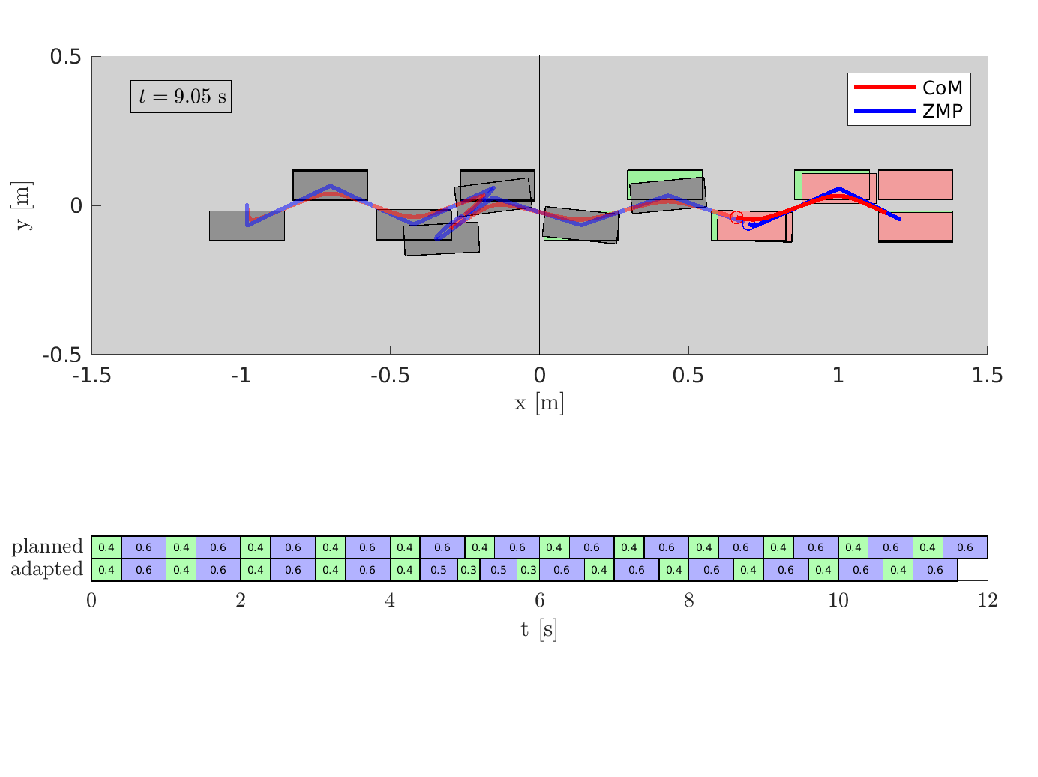
\includegraphics[trim={0 2.2cm 0 8.6cm},clip,width=\textwidth]{figures/two-patches-mixed-integer-completing-task.pdf}
    \caption{V-FAPA in the {\em 2-patches} scenario. The robot is walking
        in a straight line and is pushed at time $4.5$~s (slightly before the
        first snapshot). Now the robot is allowed to adapt the footstep position
        to the other patch, and is able to tolerate a stronger push.
    }
    \label{fig:FAPA:matlab_2pacmi}
\end{figure}

\begin{figure}
    \centering
    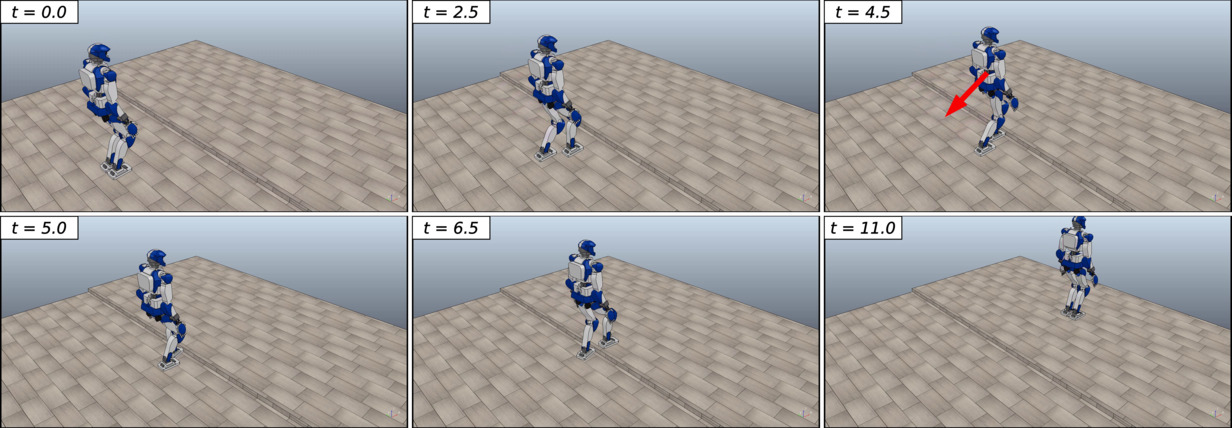
\includegraphics[width=\textwidth]{figures/two-patches-push-mixed-integer-snapshots.jpeg}
    \caption{HRP-4 walking in the \textit{2-patches} scenario using V-FAPA.
        The robot walks in a straight line and it is pushed at time 4.5 s
        (third snapshot). The robot is able to sustain the push adapting the
        footsteps and the duration of single and double support (fourth
        snapshot), eventually reaching its desired goal (last snapshot).
        Notice how the robot is able to sustain a stronger push by placing
        the foot in the first patch.
    }
    \label{fig:FAPA:sim3:snapshots}
\end{figure}

In the last simulation, the robot is moving through a more complex environment
constituted by a long staircase. While climbing, the robot is subject to
multiple pushes, triggering several footstep adjustments.
Figure \ref{fig:FAPA:sim1:snapshots} shows a sequence of snapshots of the
HRP-4 humanoid robot executing the motion.
\begin{figure}
    \centering
    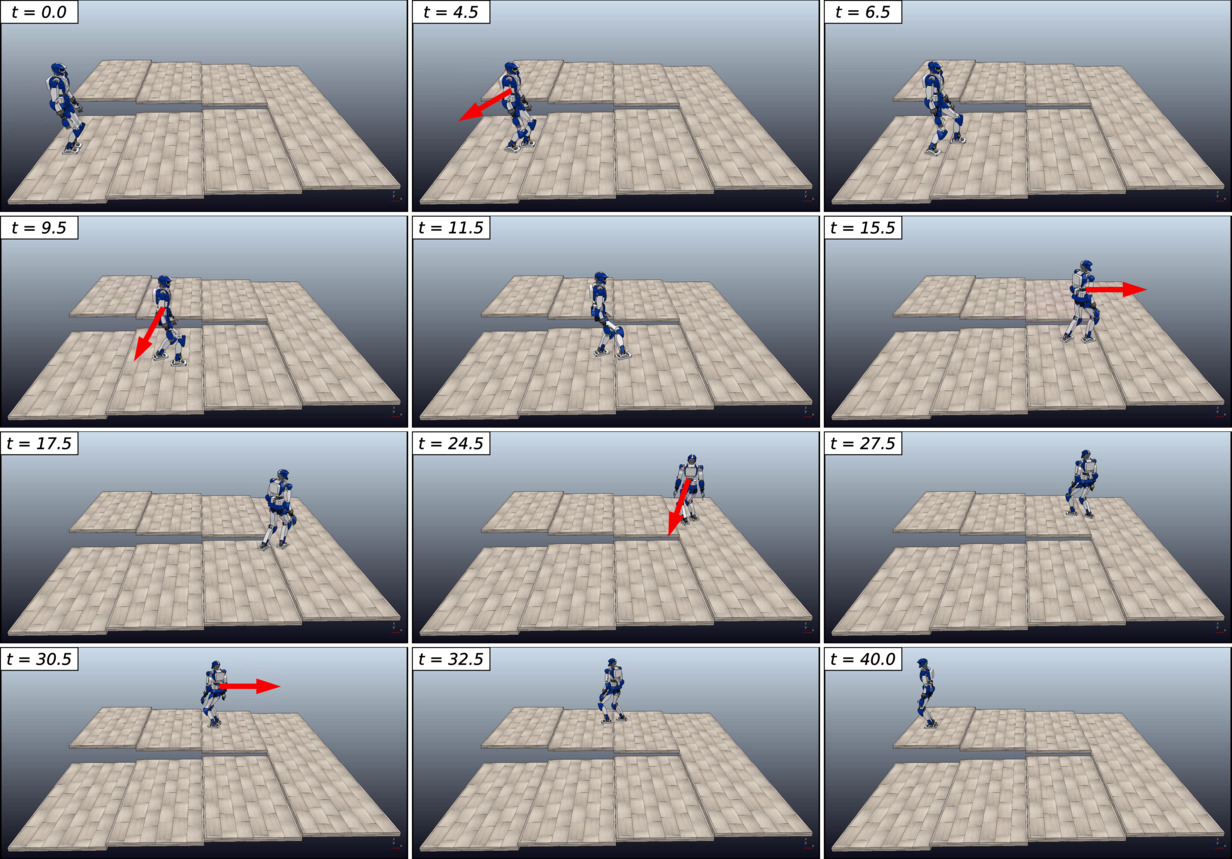
\includegraphics[width=\textwidth]{figures/staircase-multiple-pushes-snapshots.jpeg}
    \caption{HRP-4 walking in a scenario composed of multiple staircases
        using V-FAPA. The robot follows a footstep plan and it is pushed
        multiple times during the execution of the motion (second, fourth,
        sixth , eight and tenth snapshot). The robot is able to sustain
        different pushes adapting the footsteps and the duration of single
        and double support, and changing the patch when necessary.
        Eventually, the robot is able the reach the final patch.
    }
    \label{fig:FAPA:sim3:snapshots}
\end{figure}

\begin{table}
    \centering
    \begin{tabular}{*{6}{c}}
        Algorithm & Solver & Average [s] & Std dev. [s] & Max [s] \\
        \hline
        F-FAPA & \texttt{ipopt} & 0.0207 & 0.0041 & 0.0467 \\
        F-FAPA & \texttt{knitro} & 0.0144 & 0.0032 & 0.0329 \\
        V-FAPA & \texttt{bonmin} & 0.3164 & 0.2075 & 1.2098 \\
        V-FAPA & \texttt{knitro} & 0.0316 & 0.0393 & 0.3985
    \end{tabular}
    \caption{Performance metrics of F-FAPA in the {\em empty} scenario and
        V-FAPA in the {\em 2-patches} scenario, using different solvers.
    }
    \label{tab:benchmarks}
\end{table}

To discuss the real-time applicability of the scheme, we report performance
metrics in Table~\ref{tab:benchmarks}. The solvers used are \texttt{ipopt}
and \texttt{knitro} for F-FAPA, and \texttt{bonmin} and \texttt{knitro} for
V-FAPA. \texttt{knitro} is faster overall, but \texttt{ipopt} still
demonstrates good performance for F-FAPA, compatible with real-time
requirements. For V-FAPA, \texttt{bonmin} is clearly too slow, while
\texttt{knitro} has an average performance that is real-time on average,
but some outliers violate the requirements. Since all results in this chapter
are simulated, real-time performance is desirable but not critical.
However, it is necessary for hardware implementation, which is why we will
be working to guarantee real-time performance in future works.

\section{Conclusions}
\label{sec:FAPA:Conclusions}
We presented a module for adapting positions, orientations and timings in
such a way to enhance our IS-MPC scheme, using a gait feasibility constraint.
Simulated results show that the plan is adapted in a very flexible way in
reaction to strong pushes. In our MATLAB prototype, the performance is fully
compatible with real time in the case of F-FAPA, while not yet in the case of
V-FAPA. We believe that an optimized C++ implementation will be able to meet
real-time requirements. Future work will be aimed at fully accommodating these
requirements, as well as including the high-level planner
\cite{Cipriano2023RAS} inside the architecture so that global replanning
is possile.

\part{Motion control for steerable WMRs}
\chapter{Nonlinear model predictive control based on real-time iteration}
Intro.

\section{Optimal control problem and MPC formulation}
Todo.

\section{Sequential quadratic programming}
Todo.

\subsection{Direct multiple shooting}
Todo.

\section{The real-time iteration}
Todo.

\subsection{Preparation and feedback phases}
Todo.

\section{Conclusions}
Todo.
\chapter{Nonlinear model predictive control for steerable wheeled mobile robots}
\label{ch:nmpc-swmr}

\textbf{SWMR paper Abstract:}
Steerable wheeled mobile robots (SWMRs) are known to be flexibile and robust
thanks to their omnidirectionality and the presence of conventional wheels.
Nevertheless, modeling and control of this kind of platform is complex, due
to the presence of singularities in their representation or in the control
scheme. This paper proposes a framework for trajectory tracking of SWMRs using
a Nonlinear Model Predictive Control (NMPC) based on the real-time iteration
scheme, which generates feasible motions for the robot by taking into account
all kinematic singularities of the mobile base, together with bounds on driving
and steering velocities on the wheels. Our NMPC works alongside a finite state
machine and an auxiliary trajectory generation module based on dynamic feedback
linearization, which makes our framework capable of tracking any trajectory,
without ever encountering any singularity. Our approach is validated on a
Neobotix MPO-700 on trajectories of increasing difficulty.

\textbf{SWMR paper Introduction:}
In this paper, we consider the problem of trajectory tracking for steerable
wheeled mobile robots (SWMRs), equipped with an arbitrary number of wheels.
The robot is required to follow a user-defined reference pose trajectory in
an environment free of obstacles, without violating the driving and steering
velocity constraints of each wheel. Note that, in order to successfully perform
this task, it is of utmost importance to take into account the kinematic
singularities of the platform \cite{Sorour2019RAS}. In order to solve this
problem, we propose a Nonlinear MPC \cite{Rawlings2017MPCBook}, which computes
control inputs for a SWMR while tracking a reference pose trajectory,
satisfying driving and steering velocity constraints on all wheels, and handling
all kinematic singularities mentioned above. While there exists a large number
of works using MPC on differential drive robots \cite{Tarantos2023Springer},
autonomous vehicles such as cars \cite{Zanon2014Springer} and tractor trailers
\cite{Beglini2022TMECH}, and wheeled-legged robots \cite{Bjelonic2021IROS},
the application of MPC to SWMRs has yet to be explored.

\begin{figure}
    \centering
    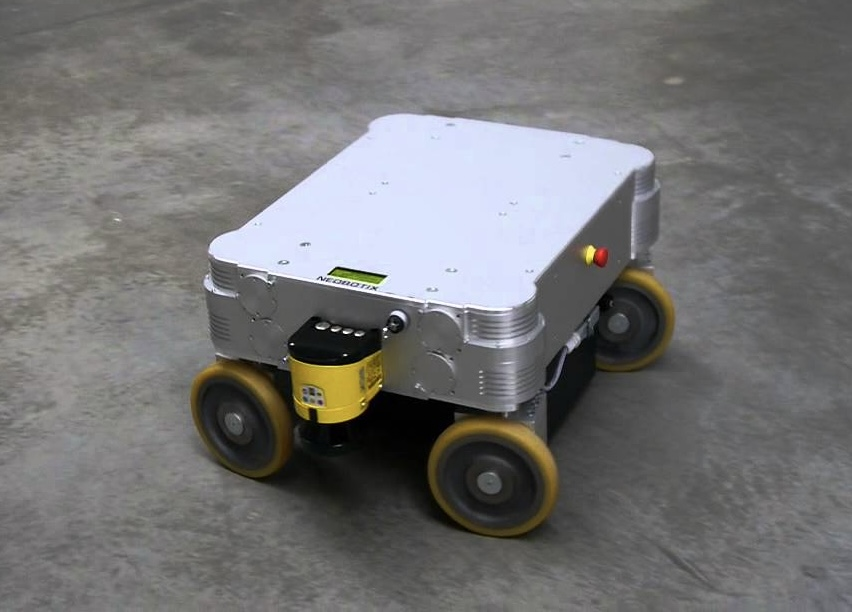
\includegraphics[width=0.7\textwidth]{figures/SWMR/mpo-700.jpg}
    \caption{The Neobotix MPO-700 steerable wheeled mobile robot.}
    \label{fig:mpo-700}
\end{figure}

Our Nonlinear MPC (NMPC) is supported by a finite state machine, which is
responsible for starting and stopping the motion of the robot while
guaranteeing that the robot never encounters any kinematic singularity, and
an auxiliary trajectory generation scheme based on dynamic feedback
linearization \cite{Oriolo2002WMRControlDFL}, which generates reference
configurations and reference control inputs for the NMPC itself, given a
user-defined reference pose trajectory. The NMPC is formulated as a Nonlinear
Programming (NLP) problem, and it is solved using the real-time iteration
\cite{Gros2020Fromlineartononlinear} scheme.

The contributions of our paper, with respect to the reviewed literature, are
the following:
\begin{itemize}
    \item we propose a framework for trajectory tracking of SWMR, which
        generates motions that satisfy driving and steering velocity bounds
        on all wheels;
    \item we present a NMPC which is intrinsically free-of-singularities
        because of the constraints (which guarantees that singularities can
        never be encountered);
    \item our NMPC is, to the best of our knowledge, the first model predictive
        control scheme to be applied to a SWMR.
\end{itemize}

Moreover, note that our framework, with respect to the taxonomy of singularities
presented in \cite{Sorour2017RAL}:
\begin{itemize}
    \item cannot encounter the singularity of the ICR being on one of the
        steerable axis because of the NMPC constraints;
    \item cannot encounter singularities due to the mobile base having zero
        velocity because of the finite state machine (which, as described
        throughout the paper, makes use of a free-of-singularities kinematic
        model);
    \item it does not present a singularity when the ICR is at infinity,
        because of the use of a different parametrization
        \cite{RobuffoGiordano2009ICRA}.
\end{itemize}  

\section{Kinematic model}
\label{sec:kinematic-model}
In this section we will develop the kinematic model of a steerable wheeled mobile robot (SWMR), following the analysis presented in \cite{RobuffoGiordano2009ICRA}. Note that while our mobile base is equipped with azimut wheels (which, in the following, we will denote as steerable wheels), the resulting kinematic model is identical to the one described in the aforementioned paper, which takes into account caster wheels.

Consider a SWMR equipped with $n_s \ge 2$ independent steerable wheels. With reference to Fig. \ref{fig:swmr}, we will denote the vector $\bm{\xi} = [x, y, \theta]^\top \in SE(2)$ as the pose of mobile base, where $(x, y)$ is its position, and $\theta$ is its orientation. Let $S_i$ be the $i$-th steering joint of the mobile base, and $W_i$ be the $i$-th wheel of the mobile base, and let $\bm{o}_{S_i}$ and $\bm{o}_{W_i}$ respectively be their positions, the latter parameterized by the steering angle $\beta_i$. Each wheel is also described by two independent velocities, the driving velocity $v_{Wi}$ and the steering velocity $v_{\beta_i}$, which are taken as control inputs. We define the whole robot configuration via the vector $\bm{q}=[\bm{\xi}^\top, \bm{\beta}^\top]^\top$, where $\bm{\beta}=[\beta_1, \dots, \beta_{n_s}]^\top$.

\begin{figure}
    \centering
    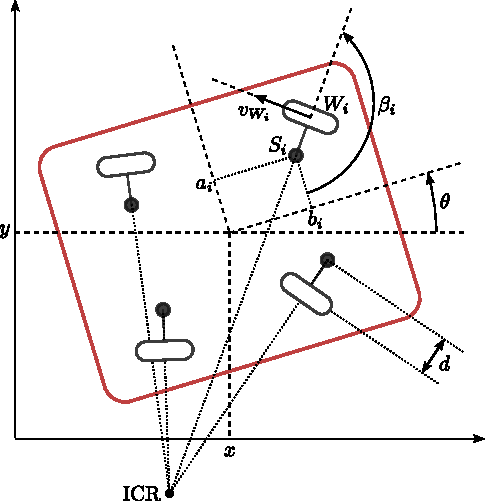
\includegraphics[width=0.65\textwidth]{figures/SWMR/swmr.pdf}
    \caption{Schematic model of a SWMR. Note that, even if the figure represents a robot equipped with four wheels, our approach is generic and works with an arbitrary number of wheels.}
    \label{fig:swmr}
\end{figure}

The position of the $i$-th steering joint $S_i$ is defined as
\begin{align*}
    \bm{o}_{S_i} &=
    \begin{bmatrix}
        x \\
        y
    \end{bmatrix}
    +
    \bm{R}(\theta)
    \begin{bmatrix}
        b_i \\
        a_i
    \end{bmatrix},
\end{align*}
and the position of the $i$-th wheel $W_i$ is defined as
\begin{align*}
    \bm{o}_{W_i} &=
    \bm{o}_{S_i}
    +
    \bm{R}(\theta + \beta_i)
    \begin{bmatrix}
        0 \\
        -d
    \end{bmatrix}.
    %\\&=
    %\begin{bmatrix}
    %    x + b_i \cos\theta - a_i \sin\theta + d \sin(\theta + \beta_i) \\
    %    y + b_i \sin\theta + a_i \cos\theta - d \cos(\theta + \beta_i),
    %\end{bmatrix}
\end{align*}
where $\bm{R} \in SO(2)$ is a rotation matrix.
%while its velocity can be defined by
%\begin{align*} 
%    \dot{\bm{o}}_{W_i} &=
%    \begin{bmatrix}
%        \dot{x} \\
%        \dot{y}
%    \end{bmatrix}
%    +
%    \dot{\bm{R}}(\theta)
%    \begin{bmatrix}
%        b_i \\
%        a_i
%    \end{bmatrix}
%    +
%    \dot{\bm{R}}(\theta + \beta_i)
%    \begin{bmatrix}
%        0 \\
%        -d
%    \end{bmatrix}
%    \\&=
%    \begin{bmatrix}
%        \dot{x} - (b_i \sin\theta + a_i \cos\theta) \dot{\theta} + d \cos(\theta + \beta_i) (\dot{\theta} + \dot{\beta}_i) \\
%        \dot{y} + (b_i \cos\theta - a_i \sin\theta) \dot{\theta} + d \sin(\theta + \beta_i) (\dot{\theta} + \dot{\beta}_i)
%    \end{bmatrix}.
%\end{align*}

Due to the assumption of no lateral skidding (i.e., the velocity of the contact point of the wheel must be orthogonal with respect to the zero motion line of the wheel itself), each wheel is subject to the Pfaffian constraint
\begin{equation}
    \label{eq:no-lateral-skidding-constraint}
    \begin{bmatrix}
        -\sin(\theta + \beta_i) \\
         \cos(\theta + \beta_i)
    \end{bmatrix}^\top \dot{\bm{o}}_{W_i} = 0.
\end{equation}
%which can be rewritten as
%\begin{equation}
%    \label{eq:no-lateral-skidding-constraint}
%    -\sin(\theta + \beta_i) \dot{x} +
%    \cos(\theta + \beta_i) \dot{y} +
%    (b_i \cos(\beta_i) + a_i \sin(\beta_i)) \dot{\theta} = 0.
%\end{equation}

By combining the above equations, it is possible to rearrange the $n_s$ nonholonomic constraints in matrix form
\begin{equation}
    \label{eq:pfaffian-constraints-matrix-form}
    \underbrace{
    \begin{bmatrix}
        -\sin(\theta + \beta_1) &
        \cos(\theta + \beta_1) &
        \Delta_1 &
        0 \dots 0 \\
        -\sin(\theta + \beta_2) &
        \cos(\theta + \beta_2) &
        \Delta_2 &
        0 \dots 0 \\
        \vdots & \vdots & \vdots & \vdots \\
        -\sin(\theta + \beta_{n_s}) &
        \cos(\theta + \beta_{n_s}) &
        \Delta_{n_s} &
        0 \dots 0 \\
    \end{bmatrix}
    }_{\bm{A}^\top(\bm{q})}
    \dot{\bm{q}} = 0,
\end{equation}
with $\Delta_i = b_i \cos\beta_i + a_i \sin\beta_i$.

In order for the mobile base to perform a motion, all wheel axles must instantaneously intersect at the same point, the ICR. The existence of an ICR can be seen as a geometric constraint, which requires all wheel orientations to be coordinated. In the following, we will study how the ICR constraint affect the mobility of the system.

\subsection{ICR constraint not satisfied}
Whenever the robot configuration is such that it has no instantaneous center of rotation (ICR), since from~(\ref{eq:pfaffian-constraints-matrix-form}) $\dot{\bm{q}} \in \mathcal{N}(\bm{A}^\top(\bm{q}))$, the kinematic model of the robot is the following:
\begin{align*}
\begin{split}
%    \dot{x} &= 0 \\
%    \dot{y} &= 0 \\
%    \dot{\theta} &= 0 \\
    \dot{\beta}_i &= v_{\beta_i},
\end{split}
\end{align*}
with $v_{\beta_i}$ steering velocities. In this case, the pose of the robot remains constant, and it is only possible to control the steering angles. 

\subsection{ICR constraint satisfied}
\label{sec:icr-constraint-satisfied}
Whenever the robot configuration is such that there exists an ICR, it is possible to simplify~\eqref{eq:pfaffian-constraints-matrix-form} through the use of coordinating functions for $\beta_i$ \cite{RobuffoGiordano2009ICRA}, with $i \ge 2$. The idea is to let the ICR be defined by the trajectory of $\bm{\xi}$, namely $\bm{\xi} \left( t \right)$. Indeed, considering the $i$-th constraint in \eqref{eq:pfaffian-constraints-matrix-form} and solving\footnote{Note that $\beta_i$ could be either $h_i(\bm{\xi}, \dot{\bm{\xi}})$ or $h_i(\bm{\xi}, \dot{\bm{\xi}}) + \pi$. In our analysis, to keep the notation simpler, we consider only the first case. However, when implementing the coordinating function, both cases need to be carefully taken into account.} for $\beta_i$ yields the coordinating function (holonomic constraint)
\begin{equation}
    \label{eq:coordinating-function-pre-kinematic-model}
    \beta_i = h_i(\bm{\xi}, \dot{\bm{\xi}}) = \mathrm{arctan} \frac{-\sin\theta\dot{x}+\cos\theta\dot{y}+b_i\dot{\theta}}{\cos\theta\dot{x}+\sin\theta\dot{y}-a_i\dot{\theta}},
\end{equation}
which can be used to ``transform'' the last $n_s-1$ constraints of \eqref{eq:pfaffian-constraints-matrix-form}, obtaining:
\begin{equation}
    \label{eq:reduced-pfaffian-constraints-matrix-form}
    \begin{bmatrix}
        -\sin(\theta + \beta_1) &
        \cos(\theta + \beta_1) &
        \Delta_1 &
        0
    \end{bmatrix}
    \begin{bmatrix}
        x \\ y \\ \theta \\ \beta_1
    \end{bmatrix}
    = 0,
\end{equation}
\begin{equation*}
    \beta_i = h_i(\bm{\xi}, \dot{\bm{\xi}}), \quad i = 2, \dots, n_s.
\end{equation*}

From \eqref{eq:reduced-pfaffian-constraints-matrix-form}, it is trivial to get the reduced kinematic model
\begin{equation}
\label{eq:reduced-kinematic-model}
\begin{split}
    \dot{x} &= v_{W_1} \cos(\theta + \beta_1) + \omega (b_1 \sin\theta + a_1 \cos\theta) \\
    \dot{y} &= v_{W_1} \sin(\theta + \beta_1) + \omega (-b_1 \cos\theta + a_1 \sin\theta) \\
    \dot{\theta} &= \omega \\
    \dot{\beta}_1 &= v_{\beta_1},
\end{split}
\end{equation}
which can be used together with \eqref{eq:coordinating-function-pre-kinematic-model} to express $\beta_i$ as
\begin{equation}
    \label{eq:coordinating-function-post-kinematic-model}
    \beta_i = h_i(v_{W_1}, \omega, \beta_1) = \mathrm{arctan} \frac{v_{W_1}\sin\beta_1+\omega(b_i-b_1)}{v_{W_1}\cos\beta_1+\omega(a_1-a_i)}.
\end{equation}

Note that the above equations (named \textit{coordinating functions}) present a singularity whenever the position of the $i$-th steering joint $S_i$ is constant (i.e., $\dot{\bm{o}}_{S_i}=\bm{0}$). This needs to be considered when designing a controller. Note that this condition is met when the platform is not moving or when the position of the ICR coincides with the position of $S_i$. 

As a consequence, if the ICR does not lie on any of the steering joints $S_i$ and if it does not change through time (i.e. $\dot{\beta}_i = 0$), all coordinating functions $h_i$ are free of singularity. Two interesting cases when these hypotheses hold are when the ICR is constant at infinity (i.e., $\omega = 0$), and when the ICR is constant, but not at infinity (i.e., $v_{W_1} = \omega R$, with $R > 0$ the distance between $\bm{o}_{W_1}$ and the ICR). In the following, we define the reduced kinematic models and the coordinating functions for these two cases, which will be used to start/stop the robot.

\begin{figure*}
    \centering
    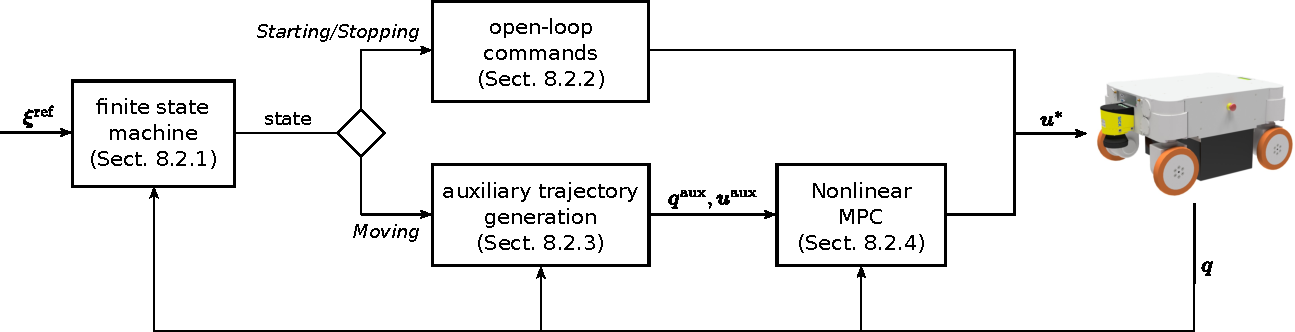
\includegraphics[width=\textwidth]{figures/SWMR/blockscheme.pdf}
    \caption{A block scheme of the proposed framework. A user-defined reference pose trajectory $\bm{\xi}^{\rm ref}$ of the mobile base is used by a FSM to determine when to start and stop the motion of the robot. As soon as a new reference trajectory is available, the state of the FSM becomes \textit{Starting}, and the mobile base is accelerated (using open-loop commands) until all wheel driving velocities are different than zero. When this condition is met, the state of the FSM becomes \textit{Moving}, and the Nonlinear MPC takes full control of the motion of the robot. In this situation, an auxiliary trajectory generation module based on dynamic feedback linearization computes the trajectories $\bm{q}^{\rm aux}$ and $\bm{u}^{\rm aux}$ (using $\bm{\xi}^{\rm ref}$), which are used by the Nonlinear MPC to compute optimal control inputs $\bm{u}^*$. The state of the FSM becomes \textit{Stopping} when $\bm{\xi}^{\rm ref} = \bm{0}$, and the robot is decelerated until it stops.}
    \label{fig:block-scheme}
\end{figure*}

\begin{figure}
    \centering
    \includegraphics[width=0.7\textwidth]{figures/SWMR/finitestatemachine.pdf}
    \caption{Finite state machine defining the motion of the mobile base.}
    \label{fig:finite-state-machine}
\end{figure}


\subsubsection{ICR constant at infinity}
\label{sec:icr-constant-at-infinity}
in the first case, we assume that the ICR exists and that it is constantly at infinity (i.e., the steering angles are the same for all wheels and $\omega = 0$). Then, the reduced kinematic model of the robot \eqref{eq:reduced-kinematic-model} becomes
\begin{align}
\label{eq:icr-constant-at-infinity-kinematic-model}
\begin{split}
    \dot{x} &= v_{W_1} \cos(\theta + \beta_1) \\
    \dot{y} &= v_{W_1} \sin(\theta + \beta_1), \\
%    \dot{\theta} &= 0 \\
%    \dot{\beta}_1 &= 0,
\end{split}
\end{align}
and the coordinating functions become $\beta_i = h_i(\beta_1) = \beta_1$. In this case, the robot can only move along a line which is parallel to the sagittal axes of the wheels.

\subsubsection{ICR constant not at infinity}
\label{sec:icr-constant-not-at-infinity}
in the second case, we assume an ICR exists and it is at a constant position (different than the position of the steering joints), but not at infinity. Then, the reduced kinematic model of the robot \eqref{eq:reduced-kinematic-model} becomes
\begin{align}
\label{eq:icr-constant-not-at-infinity-kinematic-model}
\begin{split}
    \dot{x} &= \omega R \cos(\theta + \beta_1) + \omega (b_1 \sin\theta + a_1 \cos\theta) \\
    \dot{y} &= \omega R \sin(\theta + \beta_1) + \omega (-b_1 \cos\theta + a_1 \sin\theta) \\
    \dot{\theta} &= \omega, \\
%    \dot{\beta}_1 &= 0,
\end{split}
\end{align}
and the coordinating functions become
\begin{equation*}
    \beta_i = h_i(\beta_1) = \mathrm{arctan}\frac{R \sin\beta_1 + b_i - b_1}{R \cos\beta_1 + a_1 - a_i}.
\end{equation*}
Note that $R$ can be determined from the ICR, which can be computed as the intersection point of the wheel axles. In this case, the robot can only move along the circle centered at the ICR, and radius corresponding to the distance between the position of the robot and the ICR itself. Both the center and the radius are constant, and are determined by the initial configuration of the robot.

\section{Proposed framework}
\label{sec:proposed-framework}
This section describes in detail the main components of our framework (shown in Fig. \ref{fig:block-scheme}), namely: the finite state machine, responsible for starting and stopping the robot while avoiding kinematic model singularities, the auxiliary trajectory generation module, based on dynamic feedback linearization, which provides trajectories to the NMPC, and the NMPC itself, which computes control inputs for the robot, while satisfying driving and steering velocity constraints on all wheels.

\subsection{Finite state machine}
\label{sec:finite-state-machine}
As mentioned above, since the initial configuration of the robot may be such that the ICR constraint is not satisfied, and since the NMPC must avoid configurations in which coordinating functions \eqref{eq:coordinating-function-post-kinematic-model} are singular (in order to avoid numerical instabilities), we implemented a finite state machine (FSM) to guarantee that the robot is always in a configuration free of singularity.

The FSM, shown in Fig. \ref{fig:finite-state-machine}, consists of five states (\textit{NoICR}, \textit{Ready}, \textit{Starting}, \textit{Moving} and \textit{Stopping}), described -- along with the triggering events -- hereby.
\begin{itemize}
    %\renewcommand{\labelitemi}{$\blacktriangleright$}
    \item[$\blacktriangleright$] \textit{NoICR}. The configuration of the robot is such that the ICR constraint is not satisfied. In this state, the wheels are regulated to a user-defined configuration using a proportional controller.
        \begin{itemize}
            \item[$\bullet$] Once the ICR constraint is satisfied, the state of the FSM becomes \textit{Ready}.
        \end{itemize}
    \item[$\blacktriangleright$] \textit{Ready}. The configuration of the robot is such that the ICR constraint is satisfied and the robot is not moving.
        \begin{itemize}
            \item[$\bullet$] Once a new trajectory is available, the state of the FSM becomes \textit{Starting}.
        \end{itemize}
    \item[$\blacktriangleright$] \textit{Starting}. An open loop controller makes the robot start its motion taking into account the free-of-singularities kinematic models previously presented: either \eqref{eq:icr-constant-at-infinity-kinematic-model} or \eqref{eq:icr-constant-not-at-infinity-kinematic-model} depending on the initial configuration of the robot.
        \begin{itemize}
            \item[$\bullet$] Once all velocities $\dot{\bm{o}}_{S_i}$ become non-zero, the state of the FSM becomes \textit{Moving}.
        \end{itemize}
    \item[$\blacktriangleright$] \textit{Moving}. The robot is moving using the NMPC.
        \begin{itemize}
            \item[$\bullet$] If the trajectory tracking task is about to be be completed, the state of the FSM becomes \textit{Stopping}.
        \end{itemize}
    \item[$\blacktriangleright$] \textit{Stopping}. Similarly to \textit{Starting}, an open loop motion makes the mobile base reduce its speed until it stops.
        \begin{itemize}
            \item[$\bullet$] Once the robot stops its motion, the state of the FSM becomes \textit{Ready}.
        \end{itemize}
\end{itemize}

\subsection{Starting and stopping}
\label{sec:starting-and-stopping}
In this section, we present our free-of-singularity strategy for handling starting and stopping motions. To this end, we first constrain the ICR to be constant, as already explained in Sect.~\ref{sec:icr-constraint-satisfied}, and accelerate (decelerate) the mobile base along the arc of circle defined by the initial position of the robot and the initial ICR, until all velocities $\dot{\bm{o}}_{S_i}$ are different than zero (until the robot stops its motion).

Assuming the ICR is constant at infinity, the system evolves according to~\eqref{eq:icr-constant-at-infinity-kinematic-model}. Considering the driving acceleration~$a_{W_1}$ as control input:
\begin{itemize}
    \item when the state of the FSM is \textit{Starting}, we accelerate the mobile base by choosing $a_{W_1} = a_{W_1}^{\mathrm{init}}$, where $a_{W_1}^{\mathrm{init}}$ is a hyperparameter;
    \item when the state of the FSM is \textit{Stopping}, we decelerate the mobile base by choosing $a_{W_1} = -K_{v_{W_1}}^{\mathrm{stop}} v_{W_1}$, with $K_{v_{W_1}}^{\mathrm{stop}} > 0$.
\end{itemize}

Assuming that the ICR is constant, but not at infinity and not lying on any of the steering joint positions, the system evolves according to~\eqref{eq:icr-constant-not-at-infinity-kinematic-model}.
Considering the angular acceleration $a_{\omega}$ as control input:
\begin{itemize}
    \item when the state of the FSM is \textit{Starting}, we accelerate the mobile base via $a_{\omega} = a_{W_1}^{\mathrm{init}} / R$, which, since $\dot{v}_{W_1}=a_{\omega} R$, is equivalent to accelerate $W_1$ by $a_{W_1}^{\mathrm{init}}$;
    \item when the state of the FSM is \textit{Stopping}, we decelerate the mobile base via $a_{\omega} = -K_{v_{W_1}}^{\mathrm{stop}} v_{W_1} / R$, which is equivalent to decelerate $W_1$ by $-K_{v_{W_1}}^{\mathrm{stop}} v_{W_1}$.
\end{itemize}

\subsection{Auxiliary trajectory generation}
As already mentioned, once velocities $\dot{\bm{o}}_{S_i}$ become non-zero, the state of the FSM becomes \textit{Moving}, and the robot is controlled by the NMPC. In this section, we develop an auxiliary trajectory generation module based on dynamic feedback linearization \cite{Oriolo2002WMRControlDFL}, whose purpose is to compute auxiliary configuration and control input trajectories for the NMPC, given a reference pose trajectory of the mobile base. Note that both auxiliary trajectory generation and the NMPC are only used when the state of the FSM is \textit{Moving}.

Consider the output function $\bm{z}(\bm{q})=\bm{\xi}$ and dynamically extend the robot state~\eqref{eq:reduced-kinematic-model} by adding the following integrators:
\begin{subequations}
    \begin{align*}
        \dot{v}_{W_1} &= a_{W_1} \\
        \dot{\omega} &= a_{\omega},
    \end{align*}
\end{subequations}
so that $\bm{u} = \left[ a_{W_1}, a_{\omega}, v_{\beta_1} \right]^\top $ are the new control inputs. In the following, unless specified otherwise, we denote the robot configuration with dynamic extension as $\bm{q} = (x, y, \theta, \beta_1, \beta_2, \dots, \beta_{n_s}, v_{W_1}, \omega)^\top$. Note that $\bm{q}$ is a non-minimal configuration. The dynamically extended kinematic model is
\begin{equation}
\label{eq:dynamically-extended-kinematic-model}
\begin{split}
    \dot{x} &= v_{W_1} \cos(\theta + \beta_1) + \omega (b_1 \sin\theta + a_1 \cos\theta) \\
    \dot{y} &= v_{W_1} \sin(\theta + \beta_1) + \omega (-b_1 \cos\theta + a_1 \sin\theta) \\
    \dot{\theta} &= \omega \\
    \dot{\beta}_1 &= v_{\beta_1} \\
    \dot{\beta}_i &= \dot{h}_i(\bm{q}, \bm{u}), \quad i = 2, \dots, n_s \\
    \dot{v}_{W_1} &= a_{{W_1}} \\
    \dot{\omega} &= a_{\omega},
\end{split}
\end{equation}
which, in the following, will be denoted as $\dot{\bm{q}} = \bm{f}(\bm{q}, \bm{u})$.

By deriving twice $\bm{z}(\bm{q})$, we obtain
\begin{equation}
\label{eq:zddot}
    \ddot{\bm{z}}(\bm{q})
    =
    \begin{bmatrix}
        \ddot{x} \\ \ddot{y} \\ \ddot{\theta}
    \end{bmatrix}
    =
    \bm{M}(\bm{q}) +
    \bm{H}(\bm{q})
    \begin{bmatrix}
        a_{W_1} \\ a_{\omega} \\ v_{\beta_1}
    \end{bmatrix},
\end{equation}
with $\bm{M}(\bm{q}) \in \mathbb{R}^3$ and $\bm{H}(\bm{q}) \in \mathbb{R}^{3 \times 3}$ defined as
\begin{align*}
    \bm{M}(\bm{q})
    &=
    \begin{bmatrix}
        -\sin(\theta+\beta_1) \omega v_{W_1} + ( b_1 \cos\theta - a_1 \sin\theta) \omega^2 \\
         \cos(\theta+\beta_1) \omega v_{W_1} + (-b_1 \sin\theta + a_1 \cos\theta) \omega^2 \\
        0
    \end{bmatrix}, \\
    \bm{H}(\bm{q})
    &=
    \begin{bmatrix}
        \cos(\theta+\beta_1) &  b_1 \sin\theta + a_1 \cos\theta & -\sin(\theta+\beta_1) v_{W_1} \\
        \sin(\theta+\beta_1) & -b_1 \cos\theta + a_1 \sin\theta &  \cos(\theta+\beta_1) v_{W_1} \\
        0 & 1 & 0
    \end{bmatrix}.
\end{align*}

By choosing
\begin{equation*}
    \bm{u} = \begin{bmatrix}
        a_{W_1} \\ a_{\omega} \\ v_{\beta_1}
    \end{bmatrix}
    = \bm{H}(\bm{q})^{-1} \left(\bm{a} - \bm{M}(\bm{q})\right),
\end{equation*}
it is possible to transform~\eqref{eq:zddot} into an equivalent chain of integrators
\begin{equation*}
    \ddot{\bm{z}} = \bm{a},
\end{equation*}
which can be easily stabilized. Indeed, exponential regulation of the trajectory tracking error $\bm{e}(t) = \bm{z}^{\mathrm{ref}}(t)-\bm{z}(t)$, can be achieved by taking
\begin{equation*}
    \bm{a} = \ddot{\bm{z}}^{\mathrm{ref}} + \bm{K}_P \bm{e} + \bm{K}_D \dot{\bm{e}}, \quad \bm{K}_P, \bm{K}_D > 0,
\end{equation*}
with $\bm{z}^{\mathrm{ref}}(t)$ twice differentiable and persistent (i.e., $v_{W_1} \ne 0$) reference trajectory. Note that the above decoupling matrix $\bm{H}(\bm{q})$ is singular at $v_{W_1} = 0$. This kind of singularity is structural for mobile robots \cite{Oriolo2002WMRControlDFL}.

Given the reference trajectories $\bm{\xi}^{\mathrm{ref}}, \dot{\bm{\xi}}^{\mathrm{ref}}, \ddot{\bm{\xi}}^{\mathrm{ref}}$, the scheme (Algorithm \ref{alg:AuxiliaryTrajectoryGeneration}) generates, at each timestep $t_k$, the auxiliary configurations $\bm{q}_{j|k}^{\mathrm{aux}}$ ($j = 0, \dots, N$), together with the auxiliary control inputs $\bm{u}_{j|k}^{\mathrm{aux}}$ ($j = 0, \dots, N-1$). These will be used by the NMPC, described in the next section, to compute control inputs $(a_{W_1, k}, a_{\omega, k}, v_{\beta_1, k})^T$ for the mobile base. Note that the function $\mathrm{Sample}$ discretizes a trajectory given over a time interval $[t_k, t_{k} + N \delta_{\mathrm{MPC}}]$, into $N + 1$ elements, with $\delta_{\mathrm{MPC}}$ timestep of the NMPC, and the function $\bm{F}$ integrates the dynamically extended kinematic model \eqref{eq:dynamically-extended-kinematic-model} using fourth-order Runge-Kutta over a timestep $\delta_{\mathrm{MPC}}$, considering coordinating functions \eqref{eq:coordinating-function-post-kinematic-model} for the coordinated steerable wheels $\beta_2, \dots, \beta_{n_s}$.

\begin{algorithm}
\small
\caption{AuxiliaryTrajectoryGeneration}
\label{alg:AuxiliaryTrajectoryGeneration}
\KwIn{$\bm{\xi}^{\mathrm{ref}}, \dot{\bm{\xi}}^{\mathrm{ref}}, \ddot{\bm{\xi}}^{\mathrm{ref}}$}
\KwOut{$\bm{q}_{0|k}^{\mathrm{aux}}, \dots, \bm{q}_{N|k}^{\mathrm{aux}}, \bm{u}_{0|k}^{\mathrm{aux}}, \dots, \bm{u}_{N-1|k}^{\mathrm{aux}}$}
\BlankLine
$\bm{\xi}_{0|k}^{\mathrm{ref}}, \dots, \bm{\xi}_{N|k}^{\mathrm{ref}} \gets \mathrm{Sample}(\bm{\xi}^{\mathrm{ref}})$\;
$\dot{\bm{\xi}}_{0|k}^{\mathrm{ref}}, \dots, \dot{\bm{\xi}}_{N|k}^{\mathrm{ref}} \gets \mathrm{Sample}(\dot{\bm{\xi}}^{\mathrm{ref}})$\;
$\ddot{\bm{\xi}}_{0|k}^{\mathrm{ref}}, \dots, \ddot{\bm{\xi}}_{N|k}^{\mathrm{ref}} \gets \mathrm{Sample}(\ddot{\bm{\xi}}^{\mathrm{ref}})$\;
$\bm{q}_{0|k}^{\mathrm{aux}} \gets \bm{q}_{0|k}^{\mathrm{ref}}$\;
\For{$j \gets 0$ \KwTo $N - 1$}{
    $\bm{a}_{j|k} \gets \ddot{\bm{z}}_{j|k}^{\mathrm{ref}} + \bm{K}_P (\bm{z}_{j|k}^{\mathrm{ref}} - \bm{z}_{j|k}) + \bm{K}_D (\dot{\bm{z}}_{j|k}^{\mathrm{ref}} - \dot{\bm{z}}_{j|k})$\;
    $\bm{u}_{j|k}^{\mathrm{aux}} \gets \bm{H}(\bm{q}_{j|k}^{\mathrm{aux}})^{-1} (\bm{a}_{j|k} - \bm{M}(\bm{q}_{j|k}^{\mathrm{aux}}))$\;
    $\bm{q}_{j+1|k}^{\mathrm{aux}} \gets \bm{F}(\bm{q}_{j+1|k}^{\mathrm{aux}}, \bm{u}_{j|k}^{\mathrm{aux}})$\;
}
\Return{$\bm{q}_{0|k}^{\mathrm{aux}}, \dots, \bm{q}_{N|k}^{\mathrm{aux}}, \bm{u}_{0|k}^{\mathrm{aux}}, \dots, \bm{u}_{N-1|k}^{\mathrm{aux}}$}\;
\end{algorithm}

%\begin{algorithm}
%\small
%\caption{CoordinateWheels}
%\KwIn{$\bm{q}$}
%\KwOut{$\bm{\beta}^{\mathrm{coord}}$}
%\BlankLine
%\For{$i \gets 2$ \KwTo $n_s$}{
%    $\beta_i \gets h_i(\bm{q})$\;
%}
%$\bm{\beta}^{\mathrm{coord}} \gets (\beta_2, \dots, \beta_{n_s})$\;
%\Return $\bm{\beta}^{\mathrm{coord}}$\;
%\end{algorithm}

\subsection{Nonlinear MPC}
\label{sec:model-predictive-control}
The Nonlinear MPC solves, at each control cycle, a finite horizon constrained OCP, taking into account the kinematic model \eqref{eq:reduced-kinematic-model}, wheel velocity and control inputs constraints, singularities of the coordinating functions \eqref{eq:coordinating-function-post-kinematic-model}, and the singularity of the decoupling matrix $\bm{H}(\bm{q})$ in the auxiliary trajectory generation scheme.
In the following, we will denote as $\mathbb{I}_a^b=\{a,\, \dots,\, b\}\subset\mathbb{N}$ the subset of natural numbers containing all naturals from $a$ to $b$.

The OCP can be defined as 
\begin{equation*}
    %\label{eq:ocp-swmr}
    \begin{aligned}
        \min_{\bm{u}(\cdot)} \;\;
            & \; \Phi(\bm{q}(t_k + T_{\mathrm{MPC}})) + \int_{t_k}^{t_k + T_{\mathrm{MPC}}} \mathcal{L}(\bm{q}, \bm{u}) dt \\
            \text{s.t. } & \dot{\bm{q}} = \bm{f}(\bm{q}, \bm{u}) \\
                         & v_{W_1} \ne 0 \\
                         & v_W^- \le v_{W_i} \le v_W^+,\:  \forall i \in \mathbb{I}_2^{n_s} \\
                         %& v_W^- \le v_{W_i}(\bm{q}, \bm{u}) \le v_W^+, \forall i \in \mathbb{I}_2^{n_s} \\
                         & \dot{\bm{o}}_{S_i} \ne \bm{0},\: \forall i \in \mathbb{I}_1^{n_s} \\
                         & a_W^- \le a_{W_1} \le a_W^+ \\
                         & v_{\beta}^- \le v_{\beta_i} \le v_{\beta}^+,\: \forall i \in \mathbb{I}_1^{n_s} \\
                         %& v_{\beta}^- \le \dot{h}_i(\bm{q}, \bm{u}) \le v_{\beta}^+, \forall i \in \mathbb{I}_2^{n_s} \\
                         & \bm{q}(t_k) = \bm{q}_k,
    \end{aligned}
\end{equation*}
with $T_{\mathrm{MPC}}$ duration of the prediction horizon, stage and terminal cost respectively defined as
\begin{align*}
    \mathcal{L}(\bm{q}, \bm{u}) &= \|\bm{q}^{\mathrm{aux}} - \bm{q}\|_{\bm{W_q}}^2 + \|\bm{u}^{\mathrm{aux}} - \bm{u}\|_{\bm{W_u}}^2 \\
    \Phi(\bm{q}) &= \|\bm{q}^{\mathrm{aux}} - \bm{q}\|_{\bm{W_q}}^2,
\end{align*}
$\bm{W_q}, \bm{W_u}$ positive semi-definite weighting matrices, $v_W^-$ and $v_W^+$ min/max wheel driving velocity, $a_W^-$ and $a_W^+$ min/max wheel driving acceleration, $v_{\beta}^-$ and $v_{\beta}^+$  min/max  wheel steering velocity and $\bm{q}_k$ initial configuration.

Note that the velocity constraints are linear for the coordinating wheel (since $v_{W_1}$ and $v_{\beta_1}$ are part of $\bm{q}$) and nonlinear for the coordinated wheels. In particular, because of the assumption of no lateral skidding \eqref{eq:no-lateral-skidding-constraint}, the driving velocity of the coordinated wheels can be computed as
\begin{equation*}
    v_{W_i} = 
    \begin{bmatrix}
        \cos(\theta + \beta_i) \\
        \sin(\theta + \beta_i)
    \end{bmatrix}^\top \dot{\bm{o}}_{W_i}.
\end{equation*}
Since the steering angles of the coordinated wheels are defined as $\beta_i=h_i(v_{W_1}, \omega, \beta_1)$, the steering velocities can simply be computed as their time derivatives.

%\begin{equation}
%        v_{W_i}(\bm{q}, \bm{u}) = \cos(\theta + \beta_i) \dot{x} + \sin(\theta + \beta_i) \dot{y} + (d - a_i \cos\beta_i + b_i \sin\beta_i) \dot{\theta} + d \dot{\beta}_i.
%\end{equation}
As already mentioned, since the coordinating function $h_i$ is singular when $\dot{\bm{o}}_{S_i}=\bm{0}$, it is important to carefully design the control scheme. A simple strategy to make the NMPC free of singularities, is to never let the position of the $i$-th steering joint be at rest. Since the NMPC is activated only when changing the FSM state from \textit{Starting} to \textit{Moving}, it is possible to constrain $\dot{\bm{o}}_{S_i}$ in such a way to never be $\bm{0}$. Indeed, the constraint $\dot{\bm{o}}_{S_i} \ne \bm{0}$, with a proper change of coordinates, can be rewritten as
\begin{equation*}
    \bm{R}(\theta + \beta_i) \dot{\bm{o}}_{S_i} =
    \begin{bmatrix}
        v_{S_i} \\ 0
    \end{bmatrix} \ne \bm{0},
\end{equation*}
with
\begin{equation*}
    v_{S_i} = 
    \begin{bmatrix}
        \cos(\theta + \beta_i) \\
        \sin(\theta + \beta_i)
    \end{bmatrix}^\top \dot{\bm{o}}_{S_i}.
\end{equation*}

Hence, in order to satisfy the above inequality, we need to have $v_{S_i} \ne 0$, which is equivalent to constrain $\mathrm{sgn}(v_{S_i})$ to be constant. Note that, because of the starting motion described in Sect. \ref{sec:starting-and-stopping}, $v_{S_i}$ is either positive or negative when the NMPC is activated. This implies that the constraint will simply be
\begin{equation*}
\begin{cases}
    v_{S_i} > 0, & \text{if $v_{S_i}(t_0)>0$} \\
    v_{S_i} < 0, & \text{otherwise}
\end{cases},
\end{equation*}
with $t_0$ time of activation of the NMPC. A similar reasoning can be done for the constraint $v_{W_1} \ne 0$, which guarantees subsequent calls of the auxiliary trajectory generation module are free of singularities.

We transcribe the above OCP into a nonlinear programming problem (NLP) by using multiple shooting \cite{Bock1984MultipleShooting}. The resulting NLP is the following:
\begin{equation*}
    \begin{aligned}
        \min_{\bm{Q}_k, \bm{U}_k} \;
            & \Phi(\bm{q}_{N|k}) + \sum_{j=0}^{N-1} \mathcal{L}(\bm{q}_{j|k}, \bm{u}_{j|k}) \\
            \text{s.t. } & \bm{q}_{j+1|k} = \bm{F}(\bm{q}_{j|k}, \bm{u}_{j|k}),\: \forall j \in \mathbb{I}_0^{N-1} \\
                         & \mathrm{sgn}(v_{W_1,j|k}) = \mathrm{sgn}(v_{W_1}(t_0)),\: \forall j \in \mathbb{I}_0^N \\
                         & v_W^- \le v_{W_{i,j|k}}(\cdot) \le v_W^+,\: \forall i \in \mathbb{I}_2^{n_s}, \forall j \in \mathbb{I}_0^{N-1} \\
                         & \mathrm{sgn}(v_{S_{1,j|k}}(\cdot)) = \mathrm{sgn}(v_{S_1}(t_0)),\: \forall j \in \mathbb{I}_0^N \\
                         & \mathrm{sgn}(v_{S_{i,j|k}}(\cdot)) = \mathrm{sgn}(v_{S_i}(t_0)),\: \forall i \in \mathbb{I}_2^{n_s}, \forall j \in \mathbb{I}_0^{N-1} \\
                         & a_W^- \le a_{W_1,j|k} \le a_W^+,\: \forall j \in \mathbb{I}_0^{N-1} \\
                         & v_{\beta}^- \le v_{\beta_1,j|k} \le v_{\beta}^+,\: \forall j \in \mathbb{I}_0^{N-1} \\
                         & v_{\beta}^- \le v_{\beta_i,j|k}(\cdot) \le v_{\beta}^+,\: \forall i \in \mathbb{I}_2^{n_s}, \forall j \in \mathbb{I}_0^{N-1} \\
                         & \bm{q}_{0|k} = \bm{q}_k,
    \end{aligned}
\end{equation*}
with
\begin{align*}
\bm{Q}_k &= (\bm{q}_{0|k}^\top, \bm{q}_{1|k}^\top, \dots, \bm{q}_{N|k}^\top)^\top \\
\bm{U}_k &= (\bm{u}_{0|k}^\top, \bm{u}_{1|k}^\top, \dots, \bm{u}_{N-1|k}^\top)^\top
\end{align*}
collecting the decision variables of the NMPC at $t_k$, $T_{\mathrm{MPC}}=N\delta_{\mathrm{MPC}}$, $\delta_{\mathrm{MPC}}$ timestep of the NMPC, and the cost function evaluated using $\bm{q}_{j|k}^{\mathrm{aux}}$ ($j = 0, \dots, N$) and $\bm{u}_{j|k}^{\mathrm{aux}}$ ($j = 0, \dots, N - 1$), computed by the auxiliary trajectory generation module. Notice that, within the constraints of the NLP, we used $(\cdot)$ to denote the use of nonlinear functions.

Once the NLP is solved, the control sample $\bm{u}_{0|k}$ is extracted from $\bm{U}_k$, and it is used to compute the driving and steering velocities which realize it, that are sent to the robot.

% \subsection{NMPC}
% The above optimal control problem \eqref{eq:ocp-swmr} can be transcribed to a nonlinear programming problem by properly discretizing the cost function and the constraints.

% Discretizing $\bm{\dot{q}} = \bm{v}$:
% \begin{equation}
%     \bm{q}_{k+1} = q_k + \delta \bm{v}_k
% \end{equation}
% with $\delta = t_{k+1} - t_{k}$.

% Discretizing no lateral skidding constraint \eqref{eq:no-lateral-skidding-constraint}, when $t \in [t_k, t_{k+1}]$:
% \begin{equation}
%     \label{eq:no-lateral-skidding-constraint-discretized}
%     g_{i,k}^{\rm skid}(\bm{q}_k, \bm{v}_k) = -\sin(\theta_k + \beta_{i,k}) \dot{x}_k +
%     \cos(\theta_k + \beta_{i,k}) \dot{y}_k +
%     (b_i \cos(\beta_{i,k}) + a_i \sin(\beta_{i,k})) \dot{\theta}_k = 0
% \end{equation}

% Discretizing rolling with no slipping constraint \eqref{eq:rolling-with-no-slipping-constraint}, when $t \in [t_k, t_{k+1}]$:
% \begin{equation}
%     \begin{split}
%         \label{eq:rolling-with-no-slipping-constraint-discretized}
%         g_{i,k}^{\rm slip}(\bm{q}_k, \bm{v}_k) = \cos(\theta_k + \beta_{i,k}) \dot{x}_k +
%         \sin(\theta_k + \beta_{i,k}) \dot{y}_k + \\
%         (d  - a_i \cos(\beta_{i,k}) + b_i \sin(\beta_{i,k})) \dot{\theta}_k +
%         d \dot{\beta}_{i,k}
%         -r_w \dot{\phi}_{i,k} = 0
%     \end{split}
% \end{equation}

% It is possible to define a NMPC:
% \begin{equation}
%     \label{eq:nmpc}
%     \begin{aligned}
%         \min_{\bm{q}_k, \bm{v}_k} \;
%             & L(\bm{q}_k, \bm{v}_k) \\
%             \text{s.t. } & \bm{q}_{k+1} = q_k + \delta \bm{v}_k \\
%                          & \text{no lateral skidding constraint \eqref{eq:no-lateral-skidding-constraint-discretized}} \\
%                          & \text{rolling with no slipping constraint \eqref{eq:rolling-with-no-slipping-constraint-discretized}}
%     \end{aligned}
% \end{equation}

% \subsection{Real-time iteration}
% The NMPC \eqref{eq:nmpc} can be  efficiently solved by  using real-time iteration \cite{Gros2020Fromlineartononlinear}.

% Linearize no lateral skidding constraint \eqref{eq:no-lateral-skidding-constraint-discretized} around reference trajectory:
% \begin{equation}
%     g_{i,k}^{\rm skid}(\bm{q}_k^{\rm ref}, \bm{v}_k^{\rm ref}) +
%     \left. \frac{\partial g_{i,k}^{\rm skid}}{\partial \bm{q}} \right|_{\bm{q}_k^{\rm ref}, \bm{v}_k^{\rm ref}} (\bm{q}_k^{\rm ref} - \bm{q}_k) +
%     \left. \frac{\partial g_{i,k}^{\rm skid}}{\partial \bm{v}} \right|_{\bm{q}_k^{\rm ref}, \bm{v}_k^{\rm ref}} (\bm{v}_k^{\rm ref} - \bm{v}_k) = 0
% \end{equation}

% Linearize rolling with no slipping constraint \eqref{eq:rolling-with-no-slipping-constraint-discretized} around reference trajectory:
% \begin{equation}
%     g_{i,k}^{\rm slip}(\bm{q}_k^{\rm ref}, \bm{v}_k^{\rm ref}) +
%     \left. \frac{\partial g_{i,k}^{\rm slip}}{\partial \bm{q}} \right|_{\bm{q}_k^{\rm ref}, \bm{v}_k^{\rm ref}} (\bm{q}_k^{\rm ref} - \bm{q}_k) +
%     \left. \frac{\partial g_{i,k}^{\rm slip}}{\partial \bm{v}} \right|_{\bm{q}_k^{\rm ref}, \bm{v}_k^{\rm ref}} (\bm{v}_k^{\rm ref} - \bm{v}_k) = 0
% \end{equation}

%Considering all the above kinematic constraints in Pfaffian form and rewriting them in matrix form $\bm{A}^\top(\bm{q}) \bm{\dot{q}} = 0$:
%\begin{equation}
%    \begin{bmatrix}
%        -\sin(\theta + \beta_1) &
%        \cos(\theta + \beta_1) &
%        b_1 \cos(\beta_1) + a_1 \sin(\beta_1) &
%        0 & 0 & 0 & 0 & 0 & 0 & 0 & 0 \\
%        -\sin(\theta + \beta_2) &
%        \cos(\theta + \beta_2) &
%        b_2 \cos(\beta_2) + a_2 \sin(\beta_2) &
%        0 & 0 & 0 & 0 & 0 & 0 & 0 & 0 \\
%        -\sin(\theta + \beta_3) &
%        \cos(\theta + \beta_3) &
%        b_3 \cos(\beta_3) + a_3 \sin(\beta_3) &
%        0 & 0 & 0 & 0 & 0 & 0 & 0 & 0 \\
%        -\sin(\theta + \beta_4) &
%        \cos(\theta + \beta_4) &
%        b_4 \cos(\beta_4) + a_4 \sin(\beta_4) &
%        0 & 0 & 0 & 0 & 0 & 0 & 0 & 0 \\
%        \cos(\theta + \beta_1) &
%        \sin(\theta + \beta_1) &
%        d  - a_1 \cos(\beta_1) + b_1 \sin(\beta_1) &
%        d & -r_w & 0 & 0 & 0 & 0 & 0 & 0 \\
%        \cos(\theta + \beta_2) &
%        \sin(\theta + \beta_2) &
%        d  - a_2 \cos(\beta_2) + b_2 \sin(\beta_2) &
%        0 & 0 & d & -r_w & 0 & 0 & 0 & 0 \\
%        \cos(\theta + \beta_3) &
%        \sin(\theta + \beta_3) &
%        d  - a_3 \cos(\beta_3) + b_3 \sin(\beta_3) &
%        0 & 0 & 0 & 0 & d & -r_w & 0 & 0 \\
%        \cos(\theta + \beta_4) &
%        \sin(\theta + \beta_4) &
%        d  - a_4 \cos(\beta_4) + b_4 \sin(\beta_4) &
%        0 & 0 & 0 & 0 & 0 & 0 & d & -r_w \\
%    \end{bmatrix}
%    \bm{\dot{q}} = 0
%\end{equation}

%Let $\bm{A}_1^\top(\bm{q})$ be the left submatrix of $\bm{A}^\top(\bm{q})$ of size $8 \times 3$ and $\bm{A}_2^\top(\bm{q})$ be the right submatrix of $\bm{A}^\top(\bm{q})$ of size $8 \times 8$, then:
%\begin{equation}
%    \bm{A}_1^\top(\bm{q})
%    \begin{bmatrix}
%        \dot{x} \\
%        \dot{y} \\
%        \dot{\theta}
%    \end{bmatrix}
%    =
%    -\bm{A}_2^\top(\bm{q})
%    \begin{bmatrix}
%        \dot{\beta}_1 \\
%        \dot{\phi}_1 \\
%        \dot{\beta}_2 \\
%        \dot{\phi}_2 \\
%        \dot{\beta}_3 \\
%        \dot{\phi}_3 \\
%        \dot{\beta}_4 \\
%        \dot{\phi}_4
%    \end{bmatrix}
%\end{equation}
%which can be rewritten as:
%\begin{equation}
%    \bm{\dot{\xi}} =
%    (\bm{A}_1^\top(\bm{q}))^+ \begin{bmatrix}
%        \bm{0}_4 \\
%         r_w \bm{\dot{\phi}} - d \bm{\dot{\beta}}
%    \end{bmatrix}
%\end{equation}
%with $\bm{\dot{\xi}} = [\dot{x}, \dot{y}, \dot{\theta}]^\top$, $\bm{\dot{\phi}} = [\dot{\phi}_1, \dot{\phi}_2, \dot{\phi}_3, \dot{\phi}_4]^\top$ and $\bm{\dot{\beta}} = [\dot{\beta}_1, \dot{\beta}_2, \dot{\beta}_3, \dot{\beta}_4]^\top$. {\color{red} Why odometry model in Sorour has lateral skidding constraints missing (i.e., the $\bm{0}_4$ part)?}

%\section{Model Predictive Control}
%Idea: MPC as QP using equation of motion found in section odometry model, linear constraints on inputs (mimimum and maximum velocity), cost function on $\bm{\xi}$ and $\bm{\dot{\xi}}$. Odometry model needs to be linearized.

%\subsection{Wheel coordination}
%Since the low-level controller of the platform requires the steering velocities $\dot{\beta}_i$ and the angular velocities of the wheels $\dot{\phi}_i=v_{W_i}/r_w$ (with $r_w$ radius of the wheels), it is important to compute this quantities taking into account wheel coordination and wheel slipping.

%To avoid slipping of the wheel, the projection of the velocity of the center of the wheel along the sagittal axis of the wheel must be equal to the velocity of the wheel itself:
%\begin{equation}
%    v_{W_i} =
%    \begin{bmatrix}
%        \cos(\theta + \beta_i) \\
%        \sin(\theta + \beta_i)
%    \end{bmatrix}^\top \dot{\bm{o}}_{W_i} = r_w \dot{\phi}_i,
%\end{equation}
%hence $\dot{\phi}_i = v_{W_i}/r_w$.

\section{Experiments}
\label{sec:simulations-and-experiments}
The proposed framework has been implemented in Python, using the acados library \cite{Verschueren2021acados} to solve the aforementioned NLP with the real-time iteration scheme \cite{Gros2020Fromlineartononlinear}. The mobile base used is the Neobotix MPO-700, which is equipped with $n_s=4$ steerable wheels. The scheme runs at 75 Hz on an Intel Core i5-10210U (1.6 GHz, 8 cores) with Ubuntu 20.04 LTS.

We validate our implementation on a series of trajectory tracking experiments with increasing complexity. In particular, we define a reference pose trajectory using a geometric path $\bm{\xi}^{\mathrm{ref}}(s)$ and a timing law $s(t)$. All timing laws $s(t)$ used below are 5-th order polynomials such that:
\begin{equation*}
s(t_0) = \dot{s}(t_0) = \dot{s}(t_f) = \ddot{s}(t_0) = \ddot{s}(t_f)=0, s(t_f)=1,
\end{equation*}
with $s \in [0, 1]$, and with $t_0$ and $t_f$ respectively initial and final time of the reference trajectory. This guarantees that all trajectories are defined with initial and final velocity set to zero, and with initial and final acceleration set to zero. In the following, we will use $t_0 = 0.0$ [s], and we will assume that the initial position of the robot is $x_0 = 0.0$~[m], $y_0 = 0.0$~[m].

The hyperparameters used are listed in Table \ref{tab:hyperparameters}. Video clips of the described experiments are included in the accompanying video. %Video clips of the described experiments are available at YOUTUBE LINK HERE.

\begin{table}
\centering
\begin{tabular}{ |c|c| } 
    \hline
    Symbol & Value \\
    \hline
    $\bm{a}$ & $(-0.19, 0.19, 0.19, -0.19)$ [m] \\
    $\bm{b}$ & $(0.24, 0.24, -0.24, -0.24)$ [m] \\
    $d$ & 0.045 [m] \\
    $a_{W_1}^{\mathrm{init}}$ & $0.1$ [m/s$^2$] \\ 
    $K_{v_{W_1}}^{\mathrm{stop}}$ & $1.0$ \\ 
    $\bm{K}_P$ & $\mathrm{diag}(4.0, 4.0, 2.0)$ \\ 
    $\bm{K}_D$ & $\mathrm{diag}(2.0, 2.0, 1.0)$ \\ 
    $N$ & 5 \\
    $\delta_{\mathrm{MPC}}$ & 0.1 [s] \\
    $\bm{W_q}$ & $\bm{I}_9$ \\ 
    $\bm{W_u}$ & $\bm{I}_3$ \\
    $v_W^-$ & -0.9 [m/s] \\
    $v_W^+$ & 0.9 [m/s] \\
    $a_W^-$ & $-0.5$ [m/s$^2$] \\ 
    $a_W^+$ & $0.5$ [m/s$^2$] \\ 
    $v_{\beta}^-$ & $-2.0$ [rad/s] \\ 
    $v_{\beta}^+$ & $2.0$ [rad/s] \\ 
    \hline
\end{tabular}
\caption{Hyperparameters used in all our experiments.}
\label{tab:hyperparameters}
\end{table}

\subsection{Straight line motions}
The \textit{forward motion} trajectory, consists in the robot moving along a straight line, without changing its orientation. It is defined by
\begin{equation*}
\renewcommand{\arraystretch}{1.3}
\begin{array}{c}
    \begin{aligned}
        x^{\mathrm{ref}}(s) &= x_0 + s (x_f - x_0) \\
        y^{\mathrm{ref}}(s) &= y_0 + s (y_f - y_0) \\
        \theta^{\mathrm{ref}}(s) &= \theta_0
    \end{aligned}  \\
    \begin{aligned}
        x_f &= x_0 + v^{\mathrm{ref}} \cos(\theta^{\mathrm{dir}}) (t_f - t_0) \\
        y_f &= y_0 + v^{\mathrm{ref}} \sin(\theta^{\mathrm{dir}}) (t_f - t_0),
     \end{aligned}
\end{array}
\end{equation*}
$\theta_{\mathrm{dir}}=\theta_0$ and $v^{\mathrm{ref}}>0$. The initial orientation of the robot is $\theta_0=0.0$ [rad], and the initial configuration of the steering angles is given by$\beta_{1,0}=\beta_{2,0}=\beta_{3,0}=\beta_{4,0}=0.0$ [rad]. Moreover, $t_f = 25.0$ [s] and $v^{\mathrm{ref}}=0.2$ [m/s]. Figure \ref{fig:experiments:forward:snapshots} shows a sequence of snapshots of the mobile base moving while tracking the considered trajectory. Figure \ref{fig:simulations:forward:inputs-and-errors} show the control inputs computed by the NMPC and the trajectory tracking error. Figure \ref{fig:simulations:forward:wheel-velocities} shows the corresponding driving and steering velocities.
\begin{figure*}
    \centering
    \includegraphics[width=\textwidth]{figures/SWMR/simulations/forward/snapshots.jpeg}
    \caption{Snapshots of the mobile base tracking a \textit{forward motion} trajectory.}
    \label{fig:experiments:forward:snapshots}
\end{figure*}
\begin{figure*}
    \centering
    \includegraphics[width=0.75\textwidth]{figures/SWMR/simulations/forward/inputs_and_errors.pdf}
    \caption{Control inputs and trajectory tracking errors for the \textit{forward motion} trajectory.}
    \label{fig:simulations:forward:inputs-and-errors}
\end{figure*}
\begin{figure*}
    \centering
    \includegraphics[width=0.75\textwidth]{figures/SWMR/simulations/forward/wheels_velocities.pdf}
    \caption{Driving and steering velocities of the four wheels for the \textit{forward motion} trajectory.}
    \label{fig:simulations:forward:wheel-velocities}
\end{figure*}

The \textit{backward motion} trajectory is defined similarly to the \textit{forward motion} trajectory, with the difference that $v^{\mathrm{ref}}<0$. The initial orientation of the robot is $\theta_0=0.0$ [rad]. Moreover, $\beta_{1,0}=\beta_{2,0}=\beta_{3,0}=\beta_{4,0}=\pi$ [rad], $t_f = 25.0$ [s] and $v^{\mathrm{ref}}=0.2$ [m/s]. Figure \ref{fig:experiments:backward:snapshots} shows a sequence of snapshots of the mobile base moving while tracking the considered trajectory. Figure \ref{fig:simulations:backward:inputs-and-errors} show the control inputs computed by the NMPC and the trajectory tracking error. Figure \ref{fig:simulations:backward:wheel-velocities} shows the corresponding driving and steering velocities.
\begin{figure*}
    \centering
    \includegraphics[width=\textwidth]{figures/SWMR/simulations/backward/snapshots.jpeg}
    \caption{Snapshots of the mobile base tracking a \textit{backward motion} trajectory.}
    \label{fig:experiments:backward:snapshots}
\end{figure*}
\begin{figure*}
    \centering
    \includegraphics[width=0.75\textwidth]{figures/SWMR/simulations/backward/inputs_and_errors.pdf}
    \caption{Control inputs and trajectory tracking errors for the \textit{backward motion} trajectory.}
    \label{fig:simulations:backward:inputs-and-errors}
\end{figure*}
\begin{figure*}
    \centering
    \includegraphics[width=0.75\textwidth]{figures/SWMR/simulations/backward/wheels_velocities.pdf}
    \caption{Driving and steering velocities of the four wheels for the \textit{backward motion} trajectory.}
    \label{fig:simulations:backward:wheel-velocities}
\end{figure*}

The \textit{diagonal motion} trajectory is defined similarly to the \textit{forward motion} trajectory, but with $\theta^{\mathrm{dir}} \ne \theta_0$. The initial orientation of the robot is $\theta_0=\pi/4$ [rad]. Moreover, $\beta_{1,0}=\beta_{2,0}=\beta_{3,0}=\beta_{4,0}=-\pi/4$ [rad], $t_f = 25.0$ [s] and $v^{\mathrm{ref}}=0.2$ [m/s]. Figure \ref{fig:experiments:diagonal:snapshots} shows a sequence of snapshots of the mobile base moving while tracking the considered trajectory. Figure \ref{fig:simulations:diagonal:inputs-and-errors} show the control inputs computed by the NMPC and the trajectory tracking error. Figure \ref{fig:simulations:diagonal:wheel-velocities} shows the corresponding driving and steering velocities.
\begin{figure*}
    \centering
    \includegraphics[width=\textwidth]{figures/SWMR/simulations/diagonal/snapshots.jpeg}
    \caption{Snapshots of the mobile base tracking a \textit{diagonal motion} trajectory.}
    \label{fig:experiments:diagonal:snapshots}
\end{figure*}
\begin{figure*}
    \centering
    \includegraphics[width=0.75\textwidth]{figures/SWMR/simulations/diagonal/inputs_and_errors.pdf}
    \caption{Control inputs and trajectory tracking errors for the \textit{diagonal motion} trajectory.}
    \label{fig:simulations:diagonal:inputs-and-errors}
\end{figure*}
\begin{figure*}
    \centering
    \includegraphics[width=0.75\textwidth]{figures/SWMR/simulations/diagonal/wheels_velocities.pdf}
    \caption{Driving and steering velocities of the four wheels for the \textit{diagonal motion} trajectory.}
    \label{fig:simulations:diagonal:wheel-velocities}
\end{figure*}

In all these experiments (\textit{forward}, \textit{backward} and \textit{diagonal motion}), the reference position of the robot is the same. The reference orientation, on the other hand, is different. Note that the robot is able to track diagonal trajectories because of the steerable wheels, which allow the mobile base behave as an omnidirectional robot.

\subsection{Circular motions}
In this section, we consider tasks in which the robot is required to follow a circle with center $(x_C, y_C)$ and radius $R > 0$. The reference position, which is in common among all circular trajectories (defined below), is given by
\begin{subequations}
    \begin{align*}
        x^{\mathrm{ref}}(s) &= x_C + R \cos(\phi + 2 \pi s) \\
        y^{\mathrm{ref}}(s) &= y_C + R \sin(\phi + 2 \pi s).
    \end{align*} 
\end{subequations}

In the \textit{circle with constant orientation} trajectory, the reference orientation is defined by
\begin{subequations}
\begin{align*}
    \theta^{\mathrm{ref}}(t) &= \theta_0,
\end{align*}
\end{subequations}
with $\theta_0=\pi$ [rad]. The initial configuration of the steering angles are given by$\beta_{1,0}=\beta_{2,0}=\beta_{3,0}=\beta_{4,0}=0.0$ [rad]. Moreover, $R=0.5$ [m], $\phi=\pi/2$ [rad], and $t_f=15.7$~[s].

Similarly to the \textit{diagonal motion}, the robot is able to track a circle while keeping its orientation constant because of the steerable wheels. This kind of motion, indeed, would not be possible with a differential drive robot.
Figure \ref{fig:experiments:circle-with-constant-orientation:snapshots} shows a sequence of snapshots of the mobile base moving while tracking the considered trajectory. Figure \ref{fig:simulations:circle-with-constant-orientation:inputs-and-errors} show the control inputs computed by the NMPC and the trajectory tracking error. Figure \ref{fig:simulations:circle-with-constant-orientation:wheel-velocities} shows the corresponding driving and steering velocities.
\begin{figure*}
    \centering
    \includegraphics[width=\textwidth]{figures/SWMR/simulations/circular_with_constant_orientation/snapshots.jpeg}
    \caption{Snapshots of the mobile base tracking a \textit{circle with constant orientation}.}
    \label{fig:experiments:circle-with-constant-orientation:snapshots}
\end{figure*}
\begin{figure*}
    \centering
    \includegraphics[width=0.8\textwidth]{figures/SWMR/simulations/circular_with_constant_orientation/inputs_and_errors.pdf}
    \caption{Control inputs and trajectory tracking errors for the \textit{circle with constant orientation} trajectory.}
    \label{fig:simulations:circle-with-constant-orientation:inputs-and-errors}
\end{figure*}
\begin{figure*}
    \centering
    \includegraphics[width=0.8\textwidth]{figures/SWMR/simulations/circular_with_constant_orientation/wheels_velocities.pdf}
    \caption{Driving and steering velocities of the four wheels for the \textit{circle with constant orientation} trajectory.}
    \label{fig:simulations:circle-with-constant-orientation:wheel-velocities}
\end{figure*}

In the \textit{circle with tangent orientation} trajectory, the reference orientation is defined by
\begin{equation}
    \theta^{\mathrm{ref}}(s) = \mathrm{atan2}\left(\frac{\partial y^{\mathrm{ref}}(s)}{\partial s}, \frac{\partial x^{\mathrm{ref}}(s)}{\partial s}\right).
    \label{eq:reference-tangent-orientation}
\end{equation}
Here, $\theta_0=\pi$ [rad], $\beta_{1,0}=\beta_{2,0}=\beta_{3,0}=\beta_{4,0}=0.0$ [rad]. Moreover, $R=0.5$ [m], $\phi=\pi/2$ [rad], and $t_f=15.7$~[s].
Figure \ref{fig:experiments:circle-with-tangent-orientation:snapshots} shows a sequence of snapshots of the robot moving while tracking this trajectory. Here, it is possible to notice how the mobile base changes its orientation according to the previously defined circle, ending up in its initial pose at the end of the motion. Figure \ref{fig:simulations:circle-with-tangent-orientation:inputs-and-errors} show the control inputs computed by the NMPC, together with the trajectory tracking error. Figure \ref{fig:simulations:circle-with-tangent-orientation:wheel-velocities} shows the corresponding driving and steering velocities. In these last two plots it is possible to appreciate the behavior of the NMPC. The trajectory tracking error is always close to zero, and the control inputs, together with steering and driving velocities of the wheels, are always within their boundaries.
\begin{figure*}
    \centering
    \includegraphics[width=\textwidth]{figures/SWMR/simulations/circular_with_tangent_orientation/snapshots.jpeg}
    \caption{Snapshots of the mobile robot tracking a \textit{circle with tangent orientation}.}
    \label{fig:experiments:circle-with-tangent-orientation:snapshots}
\end{figure*}
\begin{figure}
    \centering
    \includegraphics[width=0.75\textwidth]{figures/SWMR/simulations/circular_with_tangent_orientation/inputs_and_errors.pdf}
    \caption{Control inputs and trajectory tracking errors for the \textit{circle with tangent orientation} trajectory.}
    \label{fig:simulations:circle-with-tangent-orientation:inputs-and-errors}
\end{figure}
\begin{figure}
    \centering
    \includegraphics[width=0.75\textwidth]{figures/SWMR/simulations/circular_with_tangent_orientation/wheels_velocities.pdf}
    \caption{Driving and steering velocities of the four wheels for the \textit{circle with tangent orientation} trajectory.}
    \label{fig:simulations:circle-with-tangent-orientation:wheel-velocities}
\end{figure}

In the \textit{circle with inward orientation} trajectory, the robot is required to follow the previously defined circle, while pointing its front towards the center of the circle itself. The reference orientation is defined as
\begin{subequations}
\begin{align*}
    \theta^{\mathrm{ref}}(s) &= \mathrm{atan2}(y_C - y^{\mathrm{ref}}(s), x_C - x^{\mathrm{ref}}(s)).
\end{align*}
\end{subequations}
Here, $\theta_0=-\pi/2$ [rad], $\beta_{1,0}=\beta_{2,0}=\beta_{3,0}=\beta_{4,0}=-\pi/2$ [rad]. Moreover, $R=0.6$ [m], $\phi=\pi/2$ [rad], and $t_f=18.8$~[s].
Figure \ref{fig:experiments:circle-with-inward-orientation:snapshots} shows a sequence of snapshots of the mobile base moving while tracking the reference trajectory. In this experiment, it is possible to notice that the position of the mobile base is identical to the one of the previous section. The reference orientation, on the other hand, is such that the front of the robot points towards the center of the circle. Figure \ref{fig:simulations:circle-with-inward-orientation:inputs-and-errors} shows the control inputs computed by the NMPC and the trajectory tracking error. Figure \ref{fig:simulations:circle-with-inward-orientation:wheel-velocities} shows the corresponding driving and steering velocities.
\begin{figure*}
    \centering
    \includegraphics[width=\textwidth]{figures/SWMR/simulations/circular_with_inward_orientation/snapshots.jpeg}
    \caption{Snapshots of the mobile base tracking a \textit{circle with inward orientation}.}
    \label{fig:experiments:circle-with-inward-orientation:snapshots}
\end{figure*}
\begin{figure}
    \centering
    \includegraphics[width=0.75\textwidth]{figures/SWMR/simulations/circular_with_inward_orientation/inputs_and_errors.pdf}
    \caption{Control inputs and trajectory tracking errors for the \textit{circle with inward orientation} trajectory.}
    \label{fig:simulations:circle-with-inward-orientation:inputs-and-errors}
\end{figure}
\begin{figure}
    \centering
    \includegraphics[width=0.75\textwidth]{figures/SWMR/simulations/circular_with_inward_orientation/wheels_velocities.pdf}
    \caption{Driving and steering velocities of the four wheels for the \textit{circle with inward orientation} trajectory.}
    \label{fig:simulations:circle-with-inward-orientation:wheel-velocities}
\end{figure}

In the \textit{circle with outward orientation} trajectory, the robot is required to follow the previously defined circle, while pointing its back towards the center of the circle itself. The reference orientation is defined as
\begin{subequations}
\begin{align*}
    \theta^{\mathrm{ref}}(s) &= \mathrm{atan2}(y^{\mathrm{ref}}(s) - y_C, x^{\mathrm{ref}}(s) - x_C).
\end{align*}
\end{subequations}
Here, $\theta_0=\pi/2$ [rad], $\beta_{1,0}=\beta_{2,0}=\beta_{3,0}=\beta_{4,0}=\pi/2$ [rad]. Moreover, $R=0.6$ [m], $\phi=\pi/2$ [rad], and $t_f=18.8$~[s]. Figure \ref{fig:experiments:circle-with-outward-orientation:snapshots} shows a sequence of snapshots of the mobile base moving while tracking the considered trajectory. Figure \ref{fig:simulations:circle-with-outward-orientation:inputs-and-errors} show the control inputs computed by the NMPC and the trajectory tracking error. Figure \ref{fig:simulations:circle-with-outward-orientation:wheel-velocities} shows the corresponding driving and steering velocities.
\begin{figure*}
    \centering
    \includegraphics[width=\textwidth]{figures/SWMR/simulations/circular_with_outward_orientation/snapshots.jpeg}
    \caption{Snapshots of the mobile base tracking a \textit{circle with outward orientation}.}
    \label{fig:experiments:circle-with-outward-orientation:snapshots}
\end{figure*}
\begin{figure*}
    \centering
    \includegraphics[width=0.8\textwidth]{figures/SWMR/simulations/circular_with_outward_orientation/inputs_and_errors.pdf}
    \caption{Control inputs and trajectory tracking errors for the \textit{circle with outward orientation} trajectory.}
    \label{fig:simulations:circle-with-outward-orientation:inputs-and-errors}
\end{figure*}
\begin{figure*}
    \centering
    \includegraphics[width=0.8\textwidth]{figures/SWMR/simulations/circular_with_outward_orientation/wheels_velocities.pdf}
    \caption{Driving and steering velocities of the four wheels for the \textit{circle with outward orientation} trajectory.}
    \label{fig:simulations:circle-with-outward-orientation:wheel-velocities}
\end{figure*}

\subsection{Slalom motions}
In this section, we consider tasks in which the robot is required to follow a sinusoidal trajectory. The reference position, which is in common among all trajectories defined below, is given by
\begin{subequations}
\begin{align*}
    x^{\mathrm{ref}}(s) &= 2 \pi s \\
    y^{\mathrm{ref}}(s) &= \alpha \sin(2 \pi s).
\end{align*}
\end{subequations}

In the \textit{slalom with constant orientation} trajectory, the robot is required to follow the above defined sinusoidal trajectory while keeping its orientation constant. The reference orientation is given by
\begin{subequations}
\begin{align*}
    \theta^{\mathrm{ref}}(t) &= \theta_0.
\end{align*}
\end{subequations}
Here, the initial orientation of the robot is $\theta_0=0.0$ [rad]. Moreover, $\beta_{1,0}=\beta_{2,0}=\beta_{3,0}=\beta_{4,0}=0.0$ [rad], $\alpha=0.8$, and $t_f=31.4$~[s].

Note that, similarly to the \textit{circle with tangent orientation}, the tracking of this kind of trajectory is only possible because of the steerable wheels.
Figure \ref{fig:experiments:slalom-with-constant-orientation:snapshots} shows a sequence of snapshots of the mobile base moving while tracking the considered trajectory. Figure \ref{fig:simulations:slalom-with-constant-orientation:inputs-and-errors} show the control inputs computed by the NMPC and the trajectory tracking error. Figure \ref{fig:simulations:slalom-with-constant-orientation:wheel-velocities} shows the corresponding driving and steering velocities.
\begin{figure*}
    \centering
    \includegraphics[width=\textwidth]{figures/SWMR/simulations/slalom_with_constant_orientation/snapshots.jpeg}
    \caption{Snapshots of the mobile base tracking a \textit{slalom with constant orientation}.}
    \label{fig:experiments:slalom-with-constant-orientation:snapshots}
\end{figure*}
\begin{figure*}
    \centering
    \includegraphics[width=0.8\textwidth]{figures/SWMR/simulations/slalom_with_constant_orientation/inputs_and_errors.pdf}
    \caption{Control inputs and trajectory tracking errors for the \textit{slalom with constant orientation} trajectory.}
    \label{fig:simulations:slalom-with-constant-orientation:inputs-and-errors}
\end{figure*}
\begin{figure*}
    \centering
    \includegraphics[width=0.8\textwidth]{figures/SWMR/simulations/slalom_with_constant_orientation/wheels_velocities.pdf}
    \caption{Driving and steering velocities of the four wheels for the \textit{slalom with constant orientation} trajectory.}
    \label{fig:simulations:slalom-with-constant-orientation:wheel-velocities}
\end{figure*}

In the \textit{slalom with tangent orientation} trajectory, the robot is required to follow again the sinusoidal trajectory defined above, but while keeping its orientation tangent to the trajectory itself. The reference orientation is given by eq. \eqref{eq:reference-tangent-orientation}.
Here, the initial orientation of the robot is $\theta_0=\mathrm{atan}(\alpha)$ [rad]. Moreover, $\beta_{1,0}=\beta_{2,0}=\beta_{3,0}=\beta_{4,0}=0.0$ [rad], with $\alpha=0.8$, and $t_f=31.4$~[s].

Figure \ref{fig:experiments:slalom-with-tangent-orientation:snapshots} shows a sequence of snapshots of the mobile base moving while tracking the considered trajectory. Here, the reference position is the same as the one defined in the previous section, while the reference orientation in different. In the snapshots, it is possible to notice how the robot tracks the slalom while keeping its orientation tangent to the slalom itself. Figure \ref{fig:simulations:slalom-with-tangent-orientation:inputs-and-errors} shows the control inputs computed by the NMPC and the trajectory tracking error, which is always close to zero. Figure \ref{fig:simulations:slalom-with-tangent-orientation:wheel-velocities} shows the corresponding driving and steering velocities. Once again, the NMPC generates feasible control inputs while satisfying driving and steering velocity constraints on all wheels.
\begin{figure*}
    \centering
    \includegraphics[width=\textwidth]{figures/SWMR/simulations/slalom_with_tangent_orientation/snapshots.jpeg}
    \caption{Snapshots of the mobile base tracking a \textit{slalom with tangent orientation}.}
    \label{fig:experiments:slalom-with-tangent-orientation:snapshots}
\end{figure*}
\begin{figure}
    \centering
    \includegraphics[width=0.75\textwidth]{figures/SWMR/simulations/slalom_with_tangent_orientation/inputs_and_errors.pdf}
    \caption{Control inputs and trajectory tracking errors for the \textit{slalom with tangent orientation} trajectory.}
    \label{fig:simulations:slalom-with-tangent-orientation:inputs-and-errors}
\end{figure}
\begin{figure}
    \centering
    \includegraphics[width=0.75\textwidth]{figures/SWMR/simulations/slalom_with_tangent_orientation/wheels_velocities.pdf}
    \caption{Driving and steering velocities of the four wheels for the \textit{slalom with tangent orientation} trajectory.}
    \label{fig:simulations:slalom-with-tangent-orientation:wheel-velocities}
\end{figure}

\chapter{Conclusions}
\label{ch:conclusions}
This thesis addressed the problem of generation and control of motion for 
humanoids and steerable wheeled 
mobile robots. In particular, in the first part of the thesis
we have studied the problem of motion generation for humanoids 
in a \textit{world of stairs}, a particular uneven terrain where the contact 
surfaces are piecewise-horizontal. After introducing their dynamics in Chapter
\ref{ch:humanoid-locomotion-dynamics}, and Intrinsically-Stable Model Predictive
Control (IS-MPC) in Chapter \ref{ch:ISMPC},
we have presented a sensor-based framework for locomotion which makes use of a
footstep planner 
based on RRT* in Chapter \ref{ch:humanoid-motion-generation-WoS}, and a 
feasibility-aware plan adaptation module based on mixed-integer nonlinear
optimization in Chapter \ref{ch:FAPA}. In the second part of the thesis,
after a brief overview of Nonlinear Model Predictive Control (NMPC) based on the
real-time iteration (RTI) scheme in Chapter \ref{ch:nmpc-rti}, we have 
introduced a framework based on RTI for the control of the motion of steerable wheeled 
mobile robots (SWMRs) in Chapter \ref{ch:nmpc-swmr}. In the following, we
summarize the main scientific contributions of this manuscript, and discuss 
possible future works.

\medskip

In Chapter \ref{ch:humanoid-motion-generation-WoS},
we addressed the problem of motion generation for a humanoid
robot that must reach a certain goal region walking in a \textit{world of stairs}.
We considered two versions of such problem: the off-line and on-line case. 
In the first, the geometry of the environment is completely known in advance,
while in the second, it is reconstructed by the robot itself during motion using
an on-board sensor. In both cases, available information about the environment
is maintained in the form of an elevation map. 

For the off-line case, we proposed an architecture working in two main stages:
footstep planning and gait generation.
First, a feasible footstep plan leading to the goal region is off-line computed
using a randomized algorithm that takes into account the plan quality specified
by a given optimality criterion.
Then, an intrinsically stable MPC-based scheme computes a CoM trajectory that
realizes the found footstep sequence, while guaranteeing dynamic balance and
boundedness of the CoM with respect to the ZMP at all time instants.

For the on-line case, we proposed an extension of the architecture for the
off-line case where footstep plans are computed in parallel to gait generation
and map building.
To this end, we presented a sensor-based version of the footstep planner that
uses the knowledge about the environment incrementally acquired by the robot
during motion.

We validated the proposed architectures by providing simulation results
obtained in CoppeliaSim on the HRP-4 humanoid robot in scenarios of different
complexity.

Our future work will explore several directions, such as
\begin{enumerate}
    \item providing a formal proof of asymptotic optimality of the proposed
        footstep planner;
    \item developing a more general version of the proposed approach to deal
        with arbitrary terrains, removing the world of stairs assumption;
    \item implementing the presented architectures on a real humanoid robot;
    \item extending them to the case of large-scale and multi-floor environments.
\end{enumerate}

\medskip

In Chapter \ref{ch:FAPA}, we presented Feasibility-Aware Plan Adaptation (FAPA),
a module for adapting footstep plans (positions, orientations and timings) in
such a way to enhance the IS-MPC scheme of Chapter \ref{ch:ISMPC}. To do so,
we exploited the feasibility region of IS-MPC (Sect.
\ref{sec:ISMPC:feasibility-region}), using a gait feasibility constraint.
We considered two versions of the scheme:
Fixed patches FAPA (F-FAPA), where the regions assignment for placing the footsteps is 
fixed, and Variable patches FAPA (V-FAPA), where the regions can be selected
automatically. In F-FAPA, the optimization problem is formulated as a Nonlinear
Programming Problem (NLP), while in V-FAPA it is formulated as a mixed-integer 
NLP. We validated FAPA in MATLAB simulations, showing that the plan is adapted in a very
flexible way in reaction to strong pushes. In our MATLAB prototype,
the performance is fully compatible with real time in the case of F-FAPA,
while not yet in the case of V-FAPA.

Future works will be aimed at
\begin{enumerate}
    \item reimplementing FAPA in C++ in order to meet real-time requirements;
    \item introducing the on-line footstep planner of Chapter
        \ref{ch:humanoid-motion-generation-WoS}
        inside the architecture so that global replanning is possile;
    \item explore convex relaxation \cite{Marcucci2024ShortestPathsinGraphofConvexSets}
        and use a MIQP solver such as Gurobi \cite{GurobiOptimizerReferenceManual}
        to further speed up the computation;
    \item deploy FAPA on a real humanoid robot.
\end{enumerate}

\medskip

In Chapter \ref{ch:nmpc-swmr}, we presented a framework for trajectory tracking
for steerable wheeled mobile robots, which makes use of a Nonlinear MPC based
on real-time iteration. Our scheme is capable of tracking trajectories without
violating wheels' velocity constraints, while taking into account kinematic
model singularities. We have validated our approach on multiple trajectories
using the Neobotix MPO-700, showing that our scheme is always able to track
them. To the best of our knowledge, this is the first time a NMPC has been
implemented on a SWMR.

In our future works, we plan to extend the framework in several ways:
\begin{enumerate}
    \item extend the NMPC to a dual-arm mobile manipulators such as BAZAR robot
        \cite{Cherubini2019ACR}, making it interact with the environments with
        the arms while moving;
    \item implement a motion planning algorithm such as kinodynamic RRT*
        \cite{Webb2013KinodynamicRRTstar}, making the robot able to navigate
        autonomously in an environment with obstacles;
    \item further improve the performance of the framework by implementing it
        in C++ (while the scheme runs in real-time thanks to acados which
        compiles the NMPC, most of the time is taken by the auxiliary
        trajectory generation module, which completely relies on Python).
\end{enumerate}


%\appendix

\backmatter
% bibliography
\cleardoublepage
\phantomsection
%\bibliographystyle{sapthesis} % BibTeX style
\bibliographystyle{unsrt}
\bibliography{bibliography} % BibTeX database without .bib extension

\end{document}
